% -----------------------------------------------------------------
% => PARTIAL RESULTS 
% -----------------------------------------------------------------

\chapter{Resultados} \label{Chap:Results}

Neste capítulo são discutidos os resultados experimentais obtidos a partir de coletas de dados feitas em um estudo exploratório e em um estudo de caso. O estudo exploratório consistiu na realização de simulados preparatórios para o exame vestibular em turmas do primeiro e segundo anos do Ensino Médio de uma escola pública do interior do Amazonas. Tais experimentos concentraram-se na validação do Módulo `Analíticos', de modo que os dados coletados através de questionários de múltipla-escolha foram utilizados para alimentar as métricas de aprendizagem propostas com a finalidade de verificar as possibilidades de análise inteligente de aprendizagem e de viabilizar a comparação entre os métodos a serem comparados no estudo de caso.

O estudo de caso consistiu em três fases, de modo que foram analisados: (i) o impacto do uso de objetos tangíveis na aprendizagem, (ii) a percepção dos estudantes sobre o uso de objetos tangíveis e, (iii) estudo de viabilidade do uso de objetos tangíveis para o acompanhamento da aprendizagem através de métricas. Além disso, como parte da preparação para a avaliação experimental do método apresentado nesta tese, o planejamento do experimento foi submetido à apreciação dos comitês de ética das entidades participantes, de modo que o Certificado de Apresentação de Apreciação Ética (CAAE) n. 51513221.9.0000.5020 foi aprovado sob o parecer n. 4.981.458 e o CAAE n. 51513221.9.3001.8119 foi aprovado sob o parecer n. 5.264.862.


%Além disso, é apresentada uma proposta de estudo de caso acerca da integração dos objetos físico-virtuais de aprendizagem a plataforma proposta. Por fim, são apresentados alguns elementos dos Mapeamentos Sistemáticos feitos até o momento.

%Neste capítulo são discutidos os resultados experimentais iniciais obtidos a partir de coletas de dados feitas em simulados preparatórios para o exame vestibular em turmas do primeiro e segundo anos do ensino médio de um instituto federal. Tais experimentos concentraram-se na verificação do Módulo Analytics de modo que os dados coletados foram utilizados para alimentar as métricas de aprendizagem propostas com a finalidade de verificar as possibilidades de análise inteligente de aprendizagem. Além disso, é apresentada uma proposta de estudo de caso acerca da integração dos objetos físico-virtuais de aprendizagem a plataforma proposta. Por fim, são apresentados alguns elementos dos Mapeamentos Sistemáticos feitos até o momento.

\section{Estudo Exploratório das Métricas de Aprendizagem}\label{sec:resultados_analytics}
Para demonstrar e validar o Módulo das métricas apresentadas na Seção~\ref{section:analytics}, utilizamos a plataforma educacional proposta por~\cite{leitao:2017} que permite incluir um questionário de múltipla-escolha baseado em Web, contendo cinco alternativas possíveis para cada pergunta. Portanto, os alunos podem selecionar ou alterar suas respostas quantas vezes quiserem, enquanto o questionário estiver disponível. Além disso, existem também botões de navegação que permitem aos alunos revisar suas respostas. Como dito na Seção~\ref{section:player}, esta plataforma coleta dados de interação dos alunos com o material didático em tempo de execução, dentre os dados coletados estão: o tempo que o aluno passou em cada pergunta e quantas vezes o aluno mudou uma resposta para a mesma pergunta. 

\subsection{Sobre a coleta dos dados}
Foram feitas cinco coletas de dados em turmas do primeiro e segundo ano do ensino médio de um instituto federal, onde foram aplicados questionários simulando o exame de vestibular. Cada questionário tinha entre 40 e 44 questões abordando as seguintes disciplinas: Língua Portuguesa, Língua Inglesa, Língua Espanhola, História, Química, Física, Sociologia, Matemática, Geografia e Biologia. Além disso, os alunos tiveram no máximo quatro horas para responder a todas as perguntas.

A interação dos alunos com o questionário foi registrada em um arquivo {\it log} no formato CSV (\textit{Comma Separated Values}), onde foram registrados o ID da pergunta e o registro de data e hora de cada evento. Assim, o conjunto de eventos inclui as perguntas selecionadas e todas as respostas escolhidas. O cálculo das métricas foi implementado em Python e armazenado em um banco de dados NoSQL usando o MongoDB.

\subsection{Análise das Métricas}
\label{subsection:class_analysis}

Nesta seção, analisaremos alguns dos dados coletados de modo a permitir o conhecimento dos estudantes e da turma a fim de facilitar inferências que permitam tomadas de decisões pedagógicas. Para simplificar a análise e o entendimento, os dados utilizados nesta seção são restritos apenas a uma turma do primeiro ano do ensino médio contendo 33 alunos.

\subsubsection{Avaliando os estudantes}
Para analisar as métricas, usamos um método de distribuição de frequência para classificar os alunos em um conjunto de grupos (consulte Tabela~\ref{tab:Groups}), em que o valor de Piso é um intervalo fechado e o valor de Teto é um intervalo aberto. Este é um método muito utilizado em análise exploratória dos dados, pois, permite resumir e organizar o conjunto de dados em classes mutuamente exclusivas de modo a entender melhor a distribuição dos elementos neste conjunto.

O total de classes é dado pela raiz quadrada do total de alunos, ou seja, $k = \sqrt{33} \approx 6$. Considerando que as classes deveriam estar no intervalo $[0,1]$, a amplitude $h$ para cada uma é dada por $h = (1/k) = (1/6) = 0,1667$. É importante ressaltar que os valores de $k$ e $h$ são os mesmos para todas as métricas da Figura~\ref{fig:groups_students} porque o parâmetro básico o cálculo deste, isto é, a quantidade total de alunos, é o mesmo para todas elas. Além disso, para facilitar a comparação, convencionou-se que os valores mínimo e máximo dos conjuntos de dados corresponde ao menor e maior valores possíveis, respectivamente, $0$ e $1$.

\begin{table}[htbp]
\caption{Classes de Estudantes}
\centering
\begin{tabular}{|c|c|c|}
\hline
\multicolumn{1}{|c|}{\textbf{Classes}} & \multicolumn{1}{c|}{\textbf{Piso}} & \multicolumn{1}{c|}{\textbf{Teto}} \\ \hline
\textbf{Classe 1} & 0.0000 & 0.1667 \\ \hline
\textbf{Classe 2} & 0.1667 & 0.3333 \\ \hline
\textbf{Classe 3} & 0.3333 & 0.5000 \\ \hline
\textbf{Classe 4} & 0.5000 & 0.6667 \\ \hline
\textbf{Classe 5} & 0.6667 & 0.8333 \\ \hline
\textbf{Classe 6} & 0.8333 & 1.0000 \\ \hline
\end{tabular}
\label{tab:Groups}
\end{table}

A Figura~\ref{fig:groups_students} mostra o total de estudantes em cada classe de acordo com as métricas Nota Tradicional(\textit{NT}), Nota Ponderada(\textit{NP}), Grau de Assertividade(\textit{A}) e Nível de Compreensão do Questionário(\textit{NC}), que descrevem o desempenho dos alunos um conjunto de perguntas. Vale ressaltar que, se somarmos todas as barras de qualquer uma das métricas, o valor será sempre 33, que é a quantidade total de estudantes na turma.

\begin{figure}[htb]
	\centering
	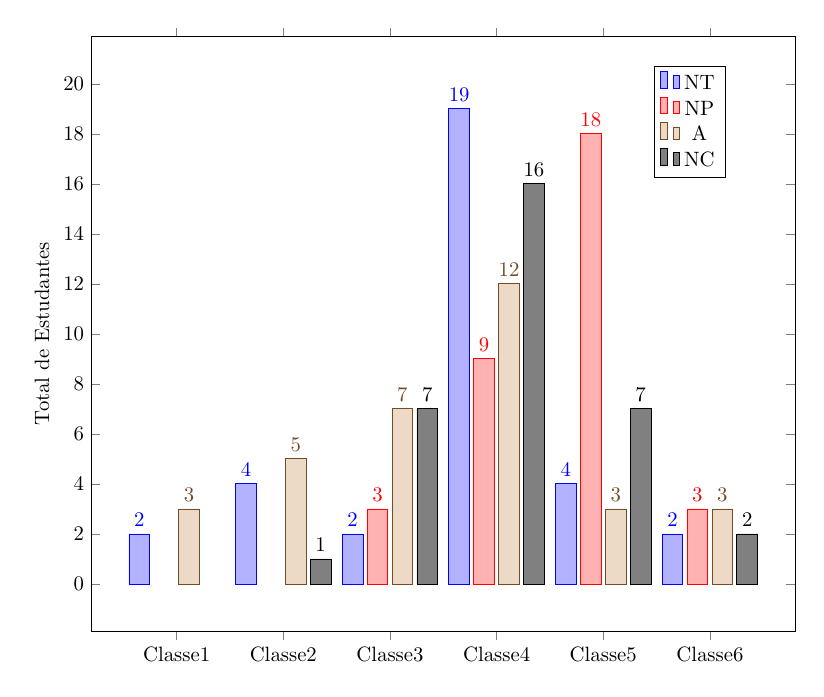
\begin{tikzpicture}[scale=0.75]
\pgfplotsset{width=13.5cm,compat=1.9}
\begin{axis}[
    ybar,
    enlargelimits=0.16,
    legend style={at={(0.85,0.95)},
      anchor=north,legend columns=1},
    ylabel={Total de Estudantes
},
    symbolic x coords={Classe1, Classe2, Classe3, Classe4, Classe5, Classe6},
    xtick=data,
    nodes near coords,
    nodes near coords align={vertical},
    ]

\addplot+[y filter/.expression={y==0 ? nan : y}] coordinates {
% TS
(Classe1,2) 
(Classe2,4) 
(Classe3,2) 
(Classe4,19) 
(Classe5, 4) 
(Classe6, 2)};

\addplot+[y filter/.expression={y==0 ? nan : y}] coordinates {
% WS
(Classe1,0)
(Classe2,0) 
(Classe3,3) 
(Classe4,9) 
(Classe5, 18)
(Classe6, 3)};

\addplot+[y filter/.expression={y==0 ? nan : y}] coordinates {
% AD
(Classe1,3)
(Classe2,5) 
(Classe3,7)
(Classe4,12)
(Classe5,3)
(Classe6,3)};

\addplot+[y filter/.expression={y==0 ? nan : y}] coordinates {
% QuCL
(Classe1,0)
(Classe2,1)
(Classe3,7)
(Classe4,16) 
(Classe5,7)
(Classe6,2)};
\legend{NT, NP, A, NC}
\end{axis}
\end{tikzpicture}
\caption{Estudantes organizados por grupos de pontuações}
     \label{fig:groups_students}
\end{figure}

Ao considerar as métricas \textit{NT}, \textit{A} e \textit{NC}, a maioria dos estudantes está nas classes 3-4 e, consequentemente, suas pontuações estão entre 0,3333 e 0,6667 (consulte os Grupos 3 e 4 na Tabela~\ref{tab:Groups}).
Por outro lado, ao considerar a métrica $NP$, a maioria dos estudantes está nas classes 4-5 e, consequentemente, suas pontuações estão entre 0,5000 e 0,8333 (consulte as Classes 4 e 5 na Tabela~\ref{tab:Groups}), indicando que essa métrica obteve uma pontuação mais alta que as outras.
No entanto, é importante notar que a métrica \textit{NT} inclui a maioria dos estudantes (19 pessoas) na Classe 4 (de 0,5000 a 0,6667); e \textit{NC} e \textit{A} mostram uma curva semelhante a uma distribuição normal.

\begin{figure}[ht]
	\centering
	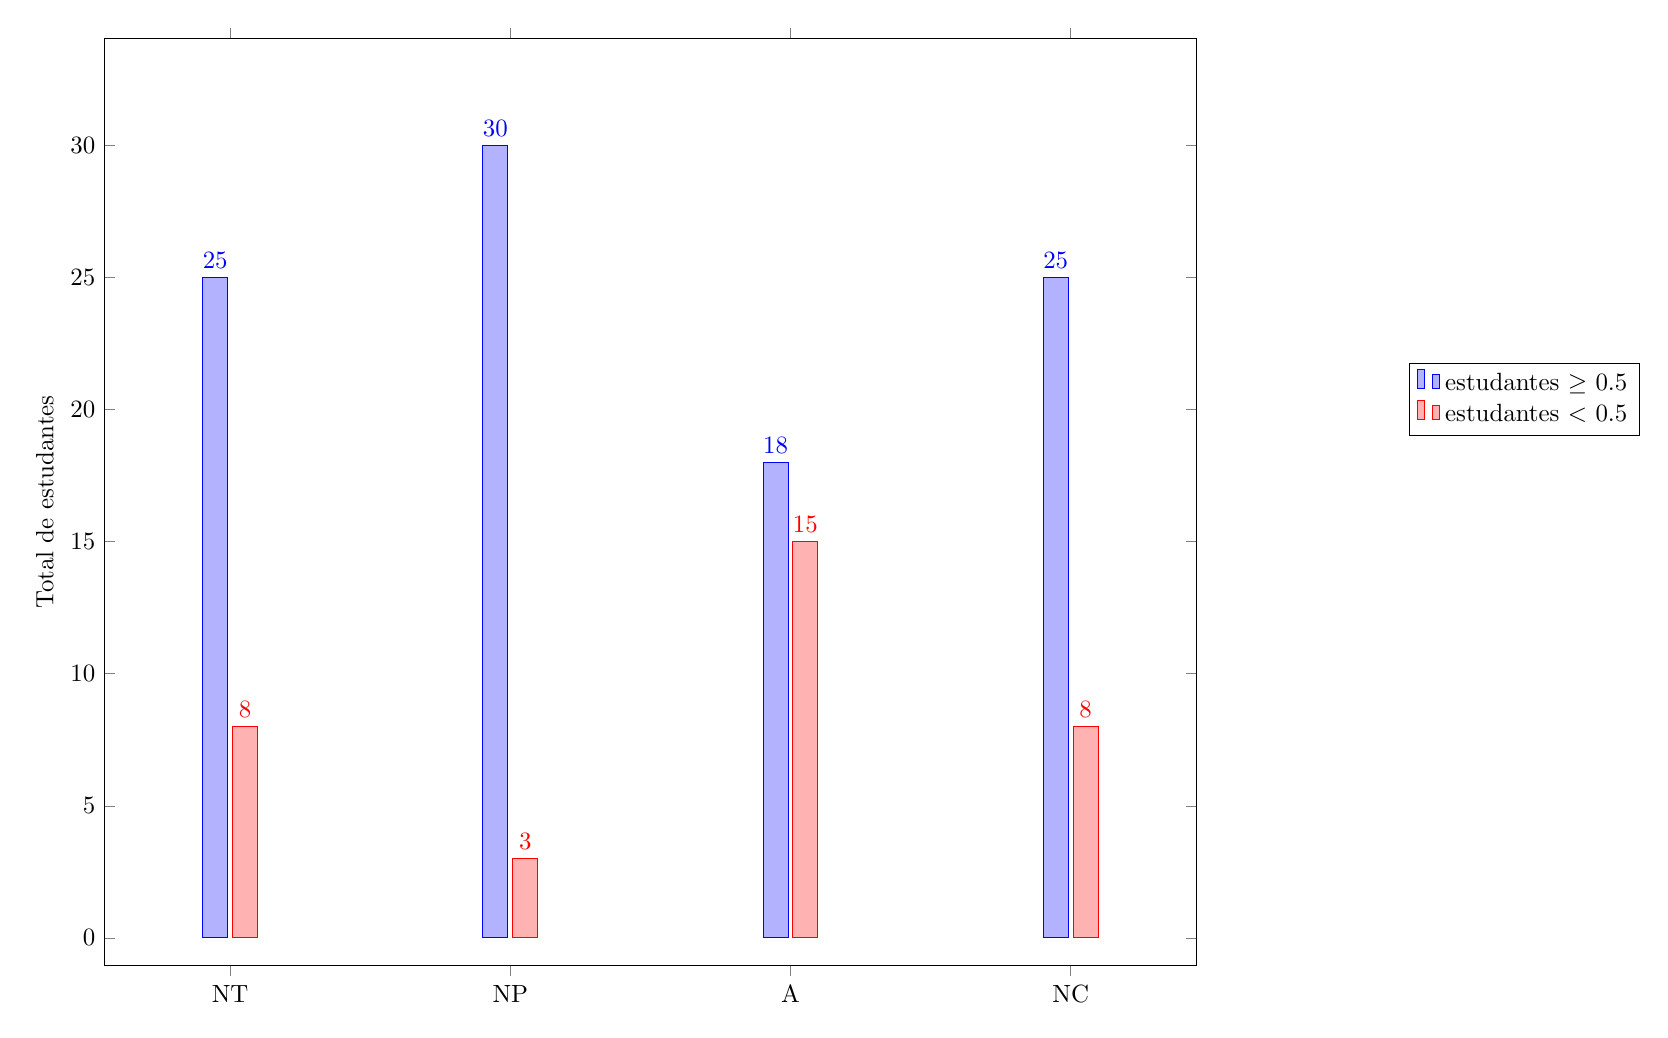
\begin{tikzpicture}[scale=0.90]
\begin{axis}[
    ybar,
    enlargelimits=0.15,
    legend style={at={(1.3,0.65)},
      anchor=north,legend columns=1},
    ylabel={Total de estudantes
},
    symbolic x coords={NT,NP,A,NC},
    xtick=data,
    nodes near coords,
    nodes near coords align={vertical},
    ]
\addplot coordinates {(NT,25) (NP,30) (A,18) (NC,25)};
\addplot coordinates {(NT,8) (NP,3) (A,15) (NC,8)};
\legend{estudantes $\geq$ 0.5, estudantes $<$ 0.5}
\end{axis}
\end{tikzpicture}
	\caption{Estudantes agrupados por situação na pontuação}
     \label{fig:students_media}
\end{figure}

A Figura~\ref{fig:students_media} apresenta a quantidade de alunos de acordo com a pontuação mínima para obter aprovação no ensino médio, ou seja, uma pontuação igual ou superior a 0,5. Primeiramente, podemos confirmar a tendência da \textit{NP} de obter uma pontuação mais alta do que outras métricas, pois trinta alunos obtiveram uma pontuação maior que 0,5. Essa característica ocorre porque essa métrica se baseia no peso da resposta, o que dá uma pontuação quando a resposta está próxima da correta.
%
Quase metade dos alunos não tem certeza absoluta de suas respostas (métrica \textit{A}). No entanto, a maioria dos alunos tem alto nível de compreensão (métrica \textit{NC}).

\subsubsection{Avaliando Disciplinas}

\begin{table}[htbp]
\caption{Prioridades das Disciplinas}
\centering
\begin{tabular}{|l|c|}
\hline
\textbf{Disciplina} & \textbf{Prioridade} \\ \hline
\textbf{Língua Inglesa} & 0.393 \\ \hline
\textbf{Geografia} & 0.373 \\ \hline
\textbf{Língua Portuguesa} & 0.322 \\ \hline
\textbf{Biologia} & 0.288 \\ \hline
\textbf{Física} & 0.260 \\ \hline
\textbf{Química} & 0.257 \\ \hline
\textbf{Matemática} & 0.240 \\ \hline
\textbf{História} & 0.205 \\ \hline
\end{tabular}
\label{tab:PrioritiesSubject}
\end{table}

\begin{table}[htbp]
\caption{Prioridades da Disciplina: Geografia}
\centering
\begin{tabular}{|l|l|}
\hline
\textbf{Dinâmica Terrestre} & 0.402 \\ \hline
\textbf{Escala} & 0.384 \\ \hline
\textbf{Cartografia} & 0.325 \\ \hline
\end{tabular}
\label{tab:PrioritiesBiology}
\end{table}

Após calcular e ordenar a média das prioridades de todos os alunos da turma, a  Tabela~\ref{tab:PrioritiesSubject} (normalizado no intervalo $[0,1]$) mostra que três as disciplinas com a maior prioridade são: Língua Inglesa (39,3\%), Geografia (37,3\%) e Língua Portuguesa (32,2\%), respectivamente. Assim, pode-se calcular os \textbf{tópicos prioritários} que cada professor pode revisar em sala de aula com todos os alunos. Por exemplo, em relação a disciplina Geografia, a Tabela~\ref{tab:PrioritiesBiology} apresenta ``Dinâmica Terrestre'' como o tópico mais prioritário, seguido por ``Escala'' e ``Cartografia'', respectivamente.

\begin{figure}[htb]
		\centering
		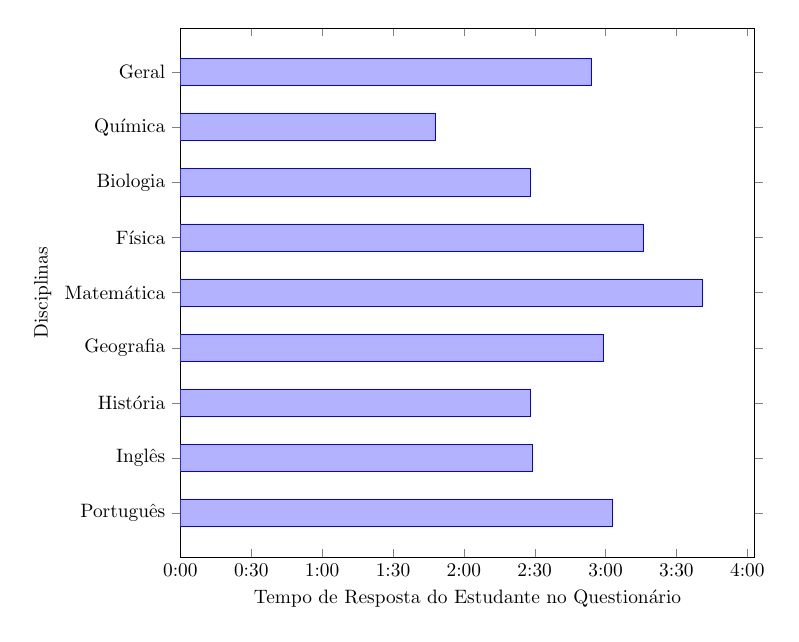
\begin{tikzpicture}[scale=0.7]
		\begin{axis}[height=10cm, width=12cm,
		xbar,
		ylabel=Disciplinas,
		xlabel=Tempo de Resposta do Estudante 
		no Questionário,
		symbolic y coords={Português,
			Inglês,
			História,
			Geografia,
			Matemática,
			Física,
			Biologia,
			Química,
			Geral},
		bar width=14pt,
		y=1.0cm,
		x filter/.code={\pgfmathparse{#1/60}},
		xticklabel={ % Split into hours and minutes
			\pgfmathsetmacro\hours{floor(\tick)}%
			\pgfmathsetmacro\minutes{(\tick-\hours)*0.6}%
			% Use some trickery to get leading zeros
			\pgfmathprintnumber{\hours}:\pgfmathprintnumber[fixed, fixed zerofill, skip 0.=true, dec sep={}]{\minutes}%
		},
		xmin=0,
		% 	xmax=225,
% 		xtick={0,0.70,...,3.8},
		]
		\addplot table{
		num values
		183 Português
		149 Inglês
		148 História
		179 Geografia
		221 Matemática
		196 Física
		148 Biologia
		108 Química
		174 Geral
		};
		\end{axis}
		\end{tikzpicture}
		\caption{Tempo médio gasto nas perguntas de cada disciplina}
		\label{fig:students_time_questionnaire}
	\end{figure}

A Figura~\ref{fig:students_time_questionnaire} mostra o tempo médio gasto em cada disciplina, de acordo com a métrica Tempo de Resposta (Seção ~\ref{section:Tempo}). Pode-se notar que Matemática, Física e Língua Portuguesa foram as disciplinas em que os alunos ocuparam mais tempo. Todas essas disciplinas estão acima da média geral das aulas.
Em relação a Língua Portuguesa, a Tabela~\ref{tab:SRTPortuguese} compara o tempo de resposta esperado com a média do tempo de resposta efetivo de todos os alunos, onde apenas as perguntas 4, 6 e 7 tiveram o tempo efetivo menor que o tempo esperado.
Essa situação diminuirá um pouco da métrica \textit{NC}, pois os alunos se encaixam no terceiro caso da Equação~\ref{eq:NCQ}, ou seja, $SRT>t$.

\begin{table}[htbp]
\caption{Tempo Gasto em Língua Portuguesa}
\centering
\begin{tabular}{|c|c|c|}
\hline
\textbf{Questões} & \textbf{TR Médio} & \textbf{Tempo Esperado (t)} \\ \hline
\textbf{Q1} & 04:47 & 03:20 \\ \hline
\textbf{Q2} & 02:50 & 02:00 \\ \hline
\textbf{Q3} & 02:58 & 01:20 \\ \hline
\textbf{Q4} & \textbf{02:17} & \textbf{03:00} \\ \hline
\textbf{Q5} & 02:49 & 01:20 \\ \hline
\textbf{Q6} & \textbf{02:18} & \textbf{03:00} \\ \hline
\textbf{Q7} & \textbf{02:46} & \textbf{03:00} \\ \hline
\textbf{Q8} & 03:38 & 03:00 \\ \hline
\textbf{Total} & 24:22 & 20:00 \\ \hline
\end{tabular}
\label{tab:SRTPortuguese}
\end{table}

%Como apresentado anteriormente na Seção~\ref{sec:disorder} (Nível de Desordem), quando a desordem é igual a zero ($D = 0$), isso significa que o aluno respondeu de maneira rígida, da primeira a última questão.
%A tabela~\ref{tab:LevelDisorderClass} apresenta a métrica Nível de Desordem ($D$) considerando todos as disciplinas. O nível de desordem é um número no intervalo $[0,1]$, mas nessa tabela é mostrado como porcentagem. As colunas são: (i) a média da desordem de cada disciplina, incluindo todos os alunos; e (ii) a porcentagem de alunos com desordem diferente de zero em relação ao tamanho da turma.

%Assim, considerando todos os estudantes, a coluna ``\textbf{Média (todos)}'' mostra que a maior desordem ocorreu na disciplina Matemática com uma média igual a 32,52\%. Além disso, na coluna ``\textbf{Percentual ($D>0$)}'', que considera apenas os alunos com desordem maior que zero, podemos ver que Matemática também tem a maior proporção de alunos com um nível de desordem, ou seja, 69,70\%.
%Este resultado pode indicar que os alunos podem ter mais dificuldades em matemática. Isso pode ser corroborado pela Figura ~\ref{fig:students_time_questionnaire}, que mostra que os alunos passaram mais tempo em matemática do que em outras disciplinas.
%
%No entanto, apesar de quase 70\% dos alunos terem respondido às perguntas fora de ordem em Matemática, seu nível de desordem, no geral, pode ser considerado baixo porque a média do nível de desordem, considerando todos os estudantes, é $32,52\%$. Esta informação deve ser considerada na análise.

%\begin{table}[htbp]
%\caption{Níveis de Desordem das Disciplinas}
%\centering
%\begin{tabular}{|l|c|c|}
%\hline
%\textbf{Disciplinas} & \textbf{Média (todos)} &  \textbf{Percentual ($D>0$)} \\ \hline
%Língua Portuguesa & 25.04\% & 54,55\% (18) \\ \hline
%Língua Inglesa & 13.44\% & 24,24\% (8)\\ \hline
%História & 31.55\% & 54,55\% (18)\\ \hline
%Geografia & 17.45\% & 33,33\% (11)\\ \hline
%Matemática & 32.52\% & 69,70\% (23)\\ \hline
%Física & 18.54\% & 36,36\% (12)\\ \hline
%Biologia & 29.62\% & 51,52\% (17)\\ \hline
%Química & 31.40\% & 54,55\% (18) \\ \hline
%%\textbf{Exam} & 35.63\% & 93,94\% \\ \hline
%\end{tabular}
%\label{tab:LevelDisorderClass}
%\end{table}
%
%Além disso, poderíamos comparar o nível de desordem com outras métricas como Grau de Assertividade (\textit{A}) e Tempo de Resposta do estudante (\textit{TR}) para verificar se a desordem alta ocorre porque os alunos estavam apenas confusos (baixo grau de assertividade) ou porque não sabiam as respostas também (desvio alto do grupo ou muito tempo gasto).

Por fim, pode-se observar na Figura~\ref{fig:students_time_questionnaire} que, no caso de Matemática, a média de tempo gasto para responder a uma pergunta é maior que todas as outras disciplinas. Também podemos observar na Tabela~\ref{tab:ADGDClass} que a média do Grau de Assertividade ($A$) da turma é de apenas 36,29\%.
Isso implica que os alunos tiveram mais dificuldade nesse assunto do que em outros, porque os estudantes passaram mais tempo e tiveram pouca segurança de resposta e alto desvio em relação às respostas corretas.

\begin{table}[htbp]
%\caption{Assurance Degree and Grouping Deviation of Subjects}
\caption{Grau de Assertividade das Disciplinas}
\centering
%\begin{tabular}{|l|c|c|}
\begin{tabular}{|l|c|}
\hline
\multicolumn{1}{|c|}{\textbf{Disciplinas}} & \textbf{A} \\ \hline % & \textbf{GD} \\ \hline
Língua Portuguesa & 0.4825 \\ \hline % & 0.3191 \\ \hline
Língua Inglesa & 0.3755 \\ \hline % & 0.3258 \\ \hline
História & 0.2446 \\ \hline % & 0.7121 \\ \hline
Geografia & 0.4162 \\ \hline % & 0.2973 \\ \hline
Matemática & 0.3629 \\ \hline % & 0.5985 \\ \hline
Física & 0.5061 \\ \hline % & 0.3977 \\ \hline
Biologia & 0.4466 \\ \hline % & 0.4413 \\ \hline
Química & 0.2611 \\ \hline % & 0.6231 \\ \hline
Geral & 0.3831 \\ \hline % & 0.4633 \\ \hline
\end{tabular}
\label{tab:ADGDClass}
\end{table}

\subsubsection{Composição das métricas: Grau de Assertividade versus Nível de Compreensão do Questionário}
\label{subsection:AD_QuCL}

Para compor as métricas do Grau de Assertividade ($A$) e do Nível de Compreensão do Questionário ($NC$), agrupamos os resultados das duas métricas em quatro grupos. O gráfico na Figura~\ref{fig:TAS_QuCL} mostra a composição. Como se pode observar, traçamos duas linhas perpendiculares nos pontos 0,5 de cada eixo, porque esta é a nota estabelecida para aprovação dos alunos na maioria das escolas de ensino médio do Brasil.

Considerando o conceito de quadrantes do Plano Cartesiano, o primeiro quadrante contém estudantes acima ou igual a 0,5 em ambas as métricas, ou seja, esses alunos têm um bom desempenho tanto em $NC$ quanto em $A$ e, por isso, não precisamos de tanta preocupação quando comparado aos estudantes nos outros quadrantes. Por exemplo, os três alunos com $NC$ maior que 0,8 têm um $A$ maior que 0,75. Isso significa que eles têm uma compreensão e confiança muito boas.

\begin{figure}[htb]
\centering
\begin{tikzpicture}
\draw[blue] (0,2.85) -- (6.85,2.85);
\draw[blue] (3.43,0) -- (3.43,5.7);
    \begin{axis}[
    % axis lines = middle,
    % enlargelimits = true,
    % axis lines=center,
    xmin=0, xmax=1,
    ymin=0, ymax=1,
    xlabel={A},
    ylabel={NC}]   
    \addplot[scatter, only marks] 
    table[x=x,y=y]{
        x    y
    0.2857	0.2839
    0.3846	0.6924
    0.5000	0.6146
    0.7500	0.8216
    0.6250	0.6829
    0.0909	0.4681
    0.8750	0.8352
    0.4444	0.5806
    0.8750	0.8432
    0.3333	0.5894
    0.5000	0.5796
    0.6000	0.4054
    0.4444	0.5347
    0.6250	0.7115
    0.6250	0.5817
    0.3636	0.6003
    0.5000	0.5225
    0.7143	0.6511
    0.4167	0.5405
    0.7500	0.7219
    0.6250	0.6855
    0.2222	0.5193
    0.2500	0.5383
    0.1739	0.4402
    0.1111	0.4389
    0.6250	0.7634
    0.1250	0.3624
    0.4444	0.5652
    0.5000	0.5447
    0.8571	0.3523
    0.5000	0.6427
    0.2857	0.3574
    0.5000	0.6639
    };
    \end{axis}
\end{tikzpicture}
     \caption{Comparação A vs. NC - Língua Portuguesa}
     \label{fig:TAS_QuCL}
 \end{figure}

Por outro lado, no terceiro quadrante, observamos os alunos em uma situação oposta, ou seja, com $NC$ e $A$ abaixo de 0,5. Essa é uma situação mais preocupante, porque os alunos têm baixos níveis de compreensão e assertividade. Na Figura~\ref{fig:TAS_QuCL}, podemos observar que todos os seis alunos deste quadrante têm um $A$ abaixo de 0,3, ou seja, eles têm um Grau de Assertividade abaixo de 30\%. O caso mais crítico de $NC$ é um aluno com 0,286. Ao analisar as duas métricas, os alunos com mais dificuldades são os três estudantes com $A$ entre 0,1 e 0,3 e $NC$ entre 0,2 e 0,4.

Os demais quadrantes têm alunos com diferentes comportamentos e necessidades. Por exemplo, no segundo quadrante, há alunos com bom $NC$ (acima de 50\%) e má confiança ($A$ abaixo de 50\%). Isso significa que esses alunos estão respondendo as perguntas corretamente, embora ainda tenham muitas dúvidas.
No entanto, esses resultados mostram que, embora esses alunos tenham muitas dúvidas, são capazes de se autocorrigir.

Finalmente, no quarto quadrante, podemos observar alunos com alto grau de assertividade, mas baixo nível de compreensão. Isso significa que esses alunos poderiam ter respondido às perguntas de maneira errada ou muito rápida, talvez tentando adivinhar. Para entender melhor cada comportamento, é necessário verificar as métricas sobre perguntas específicas ou conjunto de perguntas.

Assim, na próxima seção, analisaremos com mais detalhes o caso mais crítico.

\subsection{Analisando os estudantes do Terceiro Quadrante}\label{subsection:3rdQnd}

Conforme declarado na Seção~\ref{subsection:AD_QuCL}, a Figura~\ref{fig:TAS_QuCL} mostra que os alunos do terceiro quadrante têm baixos níveis de compreensão e assertividade e precisam de mais suporte. Por esse motivo, focaremos em alguns deles para demonstrar como as informações de novas métricas podem ser usadas para ajudar a superar suas dificuldades.

Na Tabela~\ref{tab:3rdQstudents}, comparamos as métricas dos cinco alunos com o menor $NC$ do terceiro quadrante, ou seja, valores entre 0,284 e 0,440.
Todos os dados da Tabela~\ref{tab:3rdQstudents} foram normalizados entre 0 e 1 para facilitar a comparação das métricas.
Além disso, a Figura~\ref{fig:students_time} mostra o tempo gasto pelos alunos em cada questão de Língua Portuguesa, onde os tópicos avaliados estão disponíveis na Tabela~\ref{tab:3rdQstudents_Topic}.

\begin{table}[htbp]
\caption{Estudantes com NC mais baixo}
\centering
%\begin{tabular}{|c|c|c|c|c|c|c|}
\begin{tabular}{|c|c|c|c|c|c|}
\hline
\textbf{Estudante ID} & \textbf{NT} & \textbf{NP} & %\textbf{GD} & 
\textbf{A} & \textbf{NC} & \textbf{Desordem} \\ \hline
0322 & 0.250 & 0.344 & %0.656 & 
0.286 & 0.284 & 0.000 \\ \hline
0290 & 0.500 & 0.688 & %0.313 & 
0.174 & 0.440 & 0.410 \\ \hline
0304 & 0.375 & 0.531 & %0.469 & 
0.111 & 0.439 & 0.349 \\ \hline
0320 & 0.125 & 0.406 & %0.594 & 
0.125 & 0.362 & 0.000 \\ \hline
0398 & 0.250 & 0.406 & %0.594 & 
0.286 & 0.357 & 0.000 \\ \hline
\end{tabular}
\label{tab:3rdQstudents}
\end{table}

A Tabela~\ref{tab:3rdQstudents} mostra que, para este grupo de estudantes, $NT$ está entre 0,125 e 0,500, $NP$ está entre 0,344 e 0,688, $A$ está entre 0,111 e 0,286 e apenas dois estudantes apresentaram Desordem acima de 0\%.
Vale a pena notar que um baixo grau de assertividade pode ter ocorrido não porque os alunos mudaram muito as respostas, mas porque erraram muito.

Podemos confirmar essa hipótese apenas olhando para a soma dos alunos que acertaram. Nesse caso, os dados da Tabela~\ref{tab:3rdHitsMisses} mostram que ninguém respondeu às perguntas 5 e 7, apenas um acertou as perguntas 1, 3, 6 e 8, mas as perguntas 2 e 4 foram acertadas por quatro estudantes. No entanto, apenas usando a métrica $NT$ (acertos comuns) não podemos afirmar nada sobre quais tópicos os alunos devem priorizar. Em vista disso, calculamos a métrica $P$ para esse questionário nas Tabelas~\ref{tab:3rdQstudents_Priority} e~\ref{tab:Portuguese_PriorityClass}.

\begin{table}[htbp]
\caption{Acertos (1) e erros (0) - Língua Portuguesa}
\centering
\begin{tabular}{|c|c|c|c|c|c|c|c|c|}
\hline
\multicolumn{1}{|c|}{\textbf{Estudantes}} & \textbf{Q1} & \textbf{Q2} & \textbf{Q3} & \textbf{Q4} & \textbf{Q5} & \textbf{Q6} & \textbf{Q7} & \textbf{Q8} \\ \hline
0322 & 0 & 0 & 0 & 1 & 0 & 0 & 0 & 1 \\ \hline
0290 & 1 & 1 & 1 & 1 & 0 & 0 & 0 & 0 \\ \hline
0304 & 0 & 1 & 0 & 1 & 0 & 1 & 0 & 0 \\ \hline
0320 & 0 & 1 & 0 & 0 & 0 & 0 & 0 & 0 \\ \hline
0398 & 0 & 1 & 0 & 1 & 0 & 0 & 0 & 0 \\ \hline
Total de Acertos & 1 & 4 & 1 & 4 & 0 & 1 & 0 & 1 \\ \hline
\end{tabular}
\label{tab:3rdHitsMisses}
\end{table}

\begin{table}[htbp]
\caption{Tópicos de Língua Portuguesa}
\centering
\begin{tabular}{|c|l|c|}
\hline
\textbf{ID do Tópico} & \multicolumn{1}{c|}{\textbf{Descrição}} & \textbf{Questão} \\ \hline
17 & Interpretação de Texto & 4, 7, 8 \\ \hline
81 & Ortografia & 3\\ \hline
91 & Variação Linguística & 1, 2 \\ \hline
92 & Verbo & 5, 6\\ \hline
\end{tabular}
\label{tab:3rdQstudents_Topic}
\end{table}

A Tabela~\ref{tab:3rdQstudents_Topic} mostra o ID do tópico, sua descrição e em qual pergunta este tópico foi avaliado. Na Tabela~\ref{tab:3rdQstudents_Priority}, observamos a prioridade do tópico calculado para cada aluno, em ordem decrescente. Portanto, em seu estudo pessoal, os alunos ``0322'', ``0290'' e ``0320'' devem priorizar o estudo de ``Interpretação de Texto''; o aluno ``0304'' deve se concentrar em ``Variação linguística'' e o aluno ``0398'' precisa se concentrar em ``Verbo''. Mais tarde, sugere-se aos alunos que estudem a segunda prioridade e assim por diante.

\begin{table}[htbp]
\caption{Prioridade dos Tópicos.}
\centering
\begin{tabular}{|c|l|c|l|c|l|c|l|c|}
\hline
\textbf{ID do Estudante} & \multicolumn{2}{c|}{\textbf{Prioridade 1}} & \multicolumn{2}{c|}{\textbf{Prioridade 2}} & \multicolumn{2}{c|}{\textbf{Prioridade 3}} & \multicolumn{2}{c|}{\textbf{Prioridade 4}} \\ \hline
0322 & 17 & 0.278 & 91 & 0.125 & 81 & 0.000 & 81 & 0.000 \\ \hline
0290 & 17 & 0.389 & 92 & 0.375 & 91 & 0.000 & 91 & 0.000 \\ \hline
0304 & 91 & 0.438 & 92 & 0.313 & 81 & 0.250 & 17 & 0.222 \\ \hline
0320 & 17 & 0.500 & 91 & 0.313 & 81 & 0.250 & 92 & 0.125 \\ \hline
0398 & 92 & 0.375 & 17 & 0.333 & 91 & 0.250 & 81 & 0.000 \\ \hline
\end{tabular}
\label{tab:3rdQstudents_Priority}
\end{table}

Com o objetivo de melhor apoiar o professor, no caso de uma aula de reforço para todos os alunos, a Tabela~\ref{tab:Portuguese_PriorityClass} mostra a prioridade de cada tópico para a turma (não para um aluno específico). Nesse caso, o tópico com alta prioridade é ``Variação linguística'', seguido de ``Verbo'', ``Interpretação de Texto'' e, finalmente, ``Ortografia''.

\begin{table}[htbp]
\caption{Turma - Prioridade dos Tópicos}
\centering
\begin{tabular}{|l|l|l|l|l|l|l|l|}
\hline
\multicolumn{2}{|c|}{\textbf{Prioridade 1}} & \multicolumn{2}{c|}{\textbf{Prioridade 2}} & \multicolumn{2}{c|}{\textbf{Prioridade 3}} & \multicolumn{2}{c|}{\textbf{Prioridade 4}} \\ \hline
91 & 0.342 & 92 & 0.329 & 17 & 0.323 & 81 & 0.263 \\ \hline
\end{tabular}
\label{tab:Portuguese_PriorityClass}
\end{table}

Ao considerar o tempo gasto por esses estudantes, analisando a Figura~\ref{fig:students_time}, podemos observar que alguns alunos responderam perguntas mais rapidamente que a média da turma. Em alguns casos, podemos pensar que era um chute.
Por exemplo, no caso do estudante ``0322'', questões 3 e 6; estudante ``0290'', questão 2; estudante ``0304'', questão 5; e estudante ``0398'', questão 3.

Comparando a Tabela~\ref{tab:SRTPortuguese} e a Figura~\ref{fig:students_time}, podemos ver que na Questão 2, o estudante ``0322'' excedeu o tempo em 03:22 min e o estudante ``0398'' em 03:33 min. Da mesma forma, na Questão 8, o tempo excedido foi de 01:58 e 02:50 min, respectivamente.

\begin{figure}[htb]
		\centering
		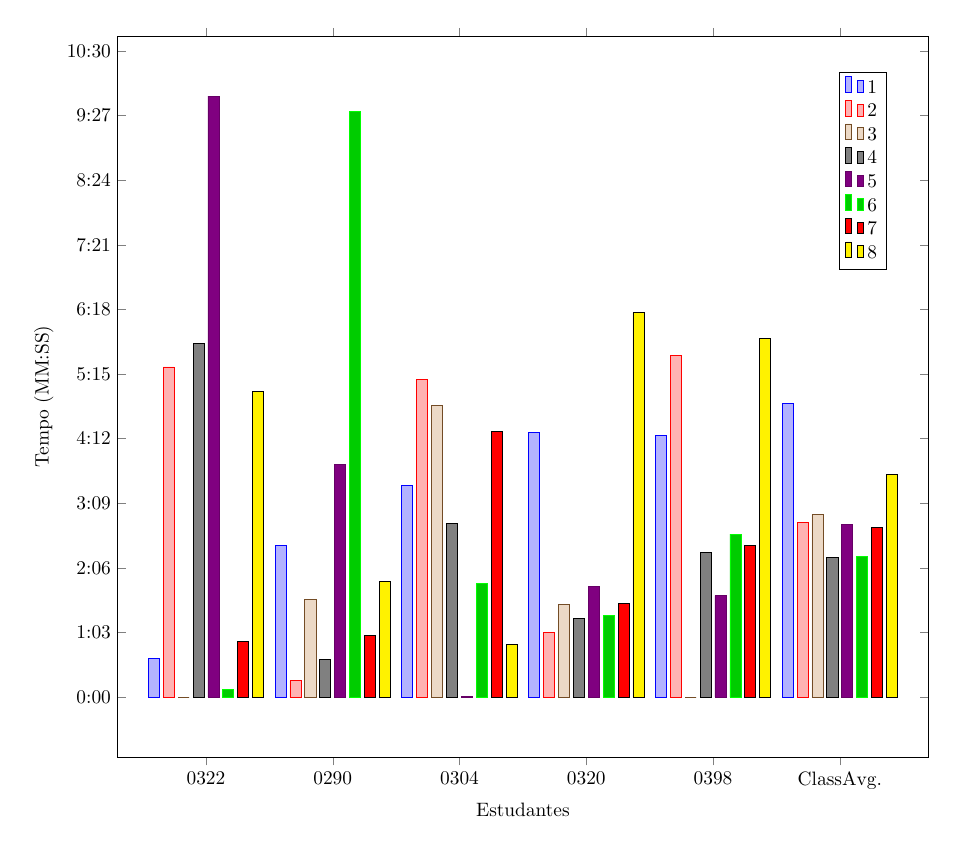
\begin{tikzpicture}[scale=0.70]
		\pgfplotsset{width=17cm,compat=newest}
		\begin{axis}[
		ybar,
		xtick=data,
		legend style={at={(0.92,0.95)},
			anchor=north,legend columns=1},
		symbolic x coords={0322, 0290, 0304, 0320, 0398, ClassAvg.},
		enlarge x limits={abs=1.6cm},
		bar width = 2.00mm,
		ylabel=Tempo (MM:SS),
		xlabel=Estudantes,
		x=2.3cm,
		y filter/.code={\pgfmathparse{#1/60}},
		yticklabel={ % Split into hours and minutes
			\pgfmathsetmacro\hours{floor(\tick)}%
			\pgfmathsetmacro\minutes{(\tick-\hours)*0.6}%
			% Use some trickery to get leading zeros
			\pgfmathprintnumber{\hours}:\pgfmathprintnumber[fixed, fixed zerofill, skip 0.=true, dec sep={}]{\minutes}%
		},
		xticklabel style=
		{rotate=0,anchor=near xticklabel},
		ytick={0,1.05,...,10.55},
		% ymin = 2009-08-18 002009-08-18 00:11:0000:00,
		]
		\addplot table {
			num value
			0322	38
			0290	148
			0304	206
			0320	258
			0398	255
			ClassAvg.	286
			
		};
		\addplot table {
			num value
			0322		322
			0290		16
			0304		310
			0320		63
			0398		333
			ClassAvg.		170
			
		};
		\addplot table {
			num value
			0322			0
			0290			95
			0304			284
			0320			90
			0398			0
			ClassAvg.			178
			
			
		};
		\addplot table {
			num value
			0322				345
			0290				37
			0304				169
			0320				77
			0398				141
			ClassAvg.				136		
		};
		\addplot table {
			num value
			0322				586
			0290				227
			0304				1
			0320				108
			0398				99
			ClassAvg.				168
			
		};
		\addplot table {
			num value
			0322					7
			0290					571
			0304					111
			0320					80
			0398					159
			ClassAvg.					137
			
		};
		\addplot[black!20!black, fill=red] table {
			num value
			0322						54
			0290						60
			0304						259
			0320						91
			0398						148
			ClassAvg.						165						
		};
		\addplot[fill=yellow] table {
			num value
			0322							298
			0290							113
			0304							51
			0320							375
			0398							350
			ClassAvg.							217	
		};
		\legend{1, 2, 3, 4, 5, 6, 7, 8}	
		\end{axis}
		\end{tikzpicture}
		\caption{Tempo gasto pelos estudantes com menor $NC$}
		\label{fig:students_time}
	\end{figure}

Observando os dados desses estudantes para essas questões específicas, podemos notar que o estudante ``0322'' acertou a Q8, mas errou a questão 2, e o contrário aconteceu com o estudante ``0398''. Assim, o tempo extra gasto nessas questões foi útil para apenas um deles. Além disso, pela Tabela~\ref{tab:QD_3rdquadrant}, a Dúvida da Questão ($DQ$) para ambos questões e estudantes era igual a zero, indicando que eles pensaram na resposta durante todo o tempo e responderam apenas uma vez. Apesar do baixo valor de $DQ$ para essas questões, o Grau de Assertividade (que é medido para o questionário inteiro) é baixo para ambos os estudantes porque, em geral, eles erraram a maioria das questões de acordo com a métrica de $NT$.

\begin{table}[htbp]
\caption{Dúvida da Questão - Estudantes com menor $NC$}
\centering
\begin{tabular}{|c|c|c|c|c|c|c|c|c|}
\hline
\textbf{Estudante} & \textbf{Q1} & \textbf{Q2} & \textbf{Q3} & \textbf{Q4} & \textbf{Q5} & \textbf{Q6} & \textbf{Q7} & \textbf{Q8} \\ \hline
0322 & 0 & 0 & -1 & 0 & 0 & 0 & 0 & 0 \\ \hline
0290 & 1 & 0 & 0 & 0 & 3 & 10 & 1 & 0 \\ \hline
0304 & 13 & 0 & 1 & 0 & 0 & 1 & 3 & 1 \\ \hline
0320 & 0 & 0 & 0 & 0 & 0 & 0 & 0 & 0 \\ \hline
0398 & 0 & 0 & -1 & 0 & 0 & 0 & 0 & 0 \\ \hline
\end{tabular}
\label{tab:QD_3rdquadrant}
\end{table}

% Para avaliar esta proposta, foi necessário implementar e testar uma plataforma experimental que auxiliasse o professor ao longo das fases do processo educativo propostas por~\cite{Zilse:2016}, isto é, as fases de composição e de execução da aula. Foi implementada ainda uma fase de avaliação a partir das métricas propostas na Seção~\ref{section:analytics} e que podem ser utilizadas para verificar se o processo educativo ocorreu conforme o planejado. Além disso, foi aplicado um questionário qualitativo ao professor com o objetivo de mensurar os impactos da plataforma a partir do ponto de vista do educador.

% Dito isto, a experimentação proposta neste capítulo visa responder às seguintes questões:
% \begin{description}
% %	\item[QP1:] É possível a construção de um ambiente de sala de aula para ensino presencial suportado por tecnologia, que possibilite a inserção de recursos computacionais dentro da metodologia normal de ensino?
% 	\item[QP1:] Quais análises e inferências podem ser feitas a partir da adição de recursos computacionais no contexto de educação?
% 	\item[QP2:] A utilização de questionários com ajuda sob demanda em processos avaliativos melhora o desempenho dos estudantes?
% 	\item[QP3:] O modelo proposto nesta dissertação auxilia satisfatoriamente o professor no uso da tecnologia para apoiar o processo de ensino-aprendizagem?
% \end{description}

% %Assim, nas seções seguintes são descritas duas aulas. Na primeira, um grupo de 15 alunos utilizou a plataforma com todos os recursos disponíveis. Na segunda, 14 alunos divididos em dois grupos heterogêneos utilizaram a plataforma, onde o primeiro grupo recebeu ajuda sob demanda proveniente da abordagem descrita nas Seções~\ref{section:composer} e~\ref{section:service} e o segundo grupo não recebeu as ajudas sob demanda.

% \section{Composição das Aulas Experimentais}\label{section:composicao_aula_experimental}

% Esta seção descreve a parte inicial dos experimentos, que coincide com a primeira fase do processo de educação, isto é, a Composição da Aula. Nesta fase, foram planejadas e executadas aulas reais da disciplina de Redes de Computadores em uma turma de Curso Técnico em Informática em uma escola do interior do Estado do Amazonas. Nesta dissertação são apresentadas duas destas aulas.

% Na primeira aula descrita (`Aula01'), um grupo de 15 estudantes utilizou a plataforma com todos os recursos disponíveis e, na segunda (`Aula02'), 14 estudantes foram divididos em dois grupos heterogêneos, onde o primeiro grupo teve acesso ao recurso das ajudas sob demanda descrito nas Seções~\ref{section:composer} e~\ref{section:service} e o segundo grupo não.

% O planejamento e a composição das aulas foram realizados a partir do modelo proposto na Seção~\ref{section:composer} em que, baseado no seu nível de dificuldade, tanto o Capítulo quanto o Assunto recebem um valor numérico a ser utilizado na métrica do nível de compreeensão. Neste caso, o professor rotulou estes dois elementos com nível de dificuldade Normal, o que significa que foi atribuído o valor 3 para tanto para o Índice de Dificuldade do Tópico (IDT), quanto para o Índice de Dificuldade do Conceito (IDC). Tendo sido utilizados os seguintes objetos de aprendizagem `Apresentação', `Vídeo', `Galeria' e `Questionário', melhor detalhados na Subseção~\ref{subsection:objetosaprendizagem}.

% \subsection{Objetos de Aprendizagem}\label{subsection:objetosaprendizagem}

% A Figura~\ref{fig:tela_aulaexperimental} apresenta a tela inicial da Aula01, onde é possível visualizar que, dos objetos de aprendizagem utilizados nessa aula, o objeto Apresentação consistiu na inserção de slides acerca dos conceitos abordados, no caso, Comutação, Roteamento e Modelos OSI e TCP/IP. O objeto Vídeo consistiu em uma animação 3D de curta-metragem sobre o roteamento e a comutação de pacotes na Internet. O objeto Galeria agregou informação histórica trazendo um conjunto de imagens com os diversos dispositivos e arquiteturas usados nas redes de comunicação de dados e de voz ao longo dos anos. O objeto Questionário contendo um conjunto de questões sobre os tópicos trabalhados anteriormente.

% \begin{figure}[ht]
% 	\centering
% 	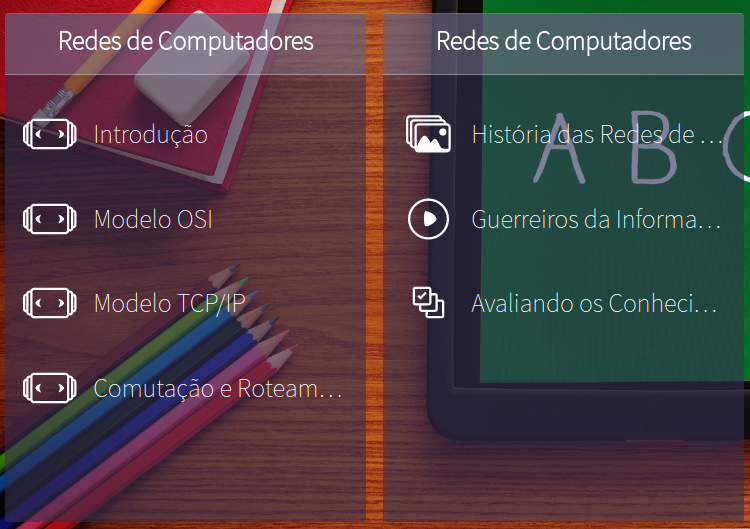
\includegraphics[width=0.8\linewidth]{imgs/aula_experimental}
% 	\caption{Tela Inicial da Aula01}
% 	\label{fig:tela_aulaexperimental}
% \end{figure}

% Na Figura~\ref{fig:tela_aulaexperimental2}, pode-se observar a inserção de dois tipos de objetos de aprendizagem: Apresentação, que consistiu em dois conjuntos de slides sobre Meios de Transmissão Guiados (que utilizam cabos) e Meios de Transmissão Não Guiados (que utilizam o ar) em Redes de Computadores e Questionário.

% \begin{figure}[ht]
% 	\centering
% 	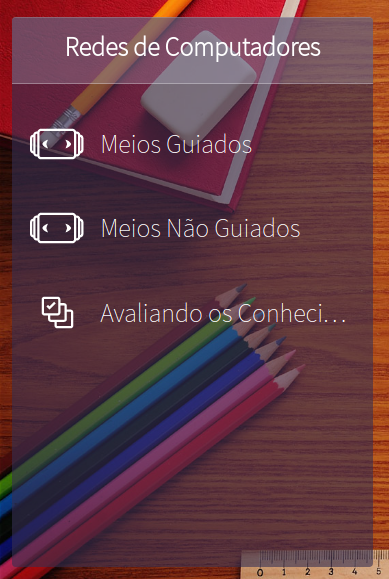
\includegraphics[width=0.4\linewidth]{imgs/aula_experimental2}
% 	\caption{Tela Inicial da Aula02}
% 	\label{fig:tela_aulaexperimental2}
% \end{figure}

% Em ambas as aulas, o objeto Questionário consistiu em um conjunto de questões avaliativas contendo 10 Questões Principais, 10 Sugestões e 10 Questões Alternativas, com conteúdo relacionado inserido na própria plataforma e presente no objeto Apresentação. Entretanto, na execução da Aula02, apenas um grupo recebeu ajuda sob demanda.

% Para um melhor entendimento do contexto das métricas utilizadas para avaliação na Seção~\ref{section:aulaexperimental}, é importante levar em consideração alguns dados sobre os questionários aplicados aos alunos. Assim, as Subseções~\ref{subsection:questionarioAula01} e~\ref{subsection:questionarioAula02} apresentam gráficos acerca das questões utilizadas.

% \subsection{Questionário da `Aula01'}\label{subsection:questionarioAula01}

% A Figura~\ref{fig:metrica_proporcao_conteudosAula01} detalha os conteúdos trabalhados e a proporção de cada um desses conteúdos no questionário aplicado à turma. Nota-se que a maior parte das questões pertence ao Tópico `Introdução' (40\%) e abarca Conceitos como representação e fluxo de dados, componentes, tipos de conexões, topologias e tipos de rede.

% O segundo tópico mais presente é `Modelo TCP/IP' (30\%) que detalha os conceitos da pilha de protocolos e dos serviços de rede baseados nessa pilha. O terceiro Tópico mais recorrente no questionário foi sobre `Comutação e Roteamento'(20\%), que aborda os conceitos de comutação de circuitos, comutação de pacotes e roteamento de pacotes. Já o Tópico `Modelo OSI' esteve presente em apenas 10\% das questões.

% \begin{figure}[ht]
% 	\centering
% 	\includegraphics[width=0.7\linewidth]{imgs/metricas/proporcao_conteudosAula01}
% 	\caption{Proporção dos Tópicos das Aulas no Questionário}
% 	\label{fig:metrica_proporcao_conteudosAula01}
% \end{figure}

% A Figura~\ref{fig:metrica_nivel_dificuldadeAula01} resume informações sobre a distribuição do nível de dificuldade das questões. Pode-se perceber que, das 10 questões, 50\% são rotuladas como Difícil, 40\% são questões de nível Normal e 10\% questões de nível Fácil. A distribuição se deu desse modo porque o professor desejava provocar um maior uso dos níveis de ajuda por parte dos estudantes.

% \begin{figure}[ht]
% 	\centering
% 	\includegraphics[width=0.8\linewidth]{imgs/metricas/nivel_dificuldades_questoesAula01}
% 	\caption{Gráfico do Nível de Dificuldade das Questões}
% 	\label{fig:metrica_nivel_dificuldadeAula01}
% \end{figure}

% A Figura~\ref{fig:metrica_dificuldade_topicosAula01} apresenta o gráfico da distribuição do nível de dificuldade das questões a partir dos Tópicos estudados na aula. Analisando esse gráfico, podemos perceber que as questões rotuladas como `Difícil' (N5) estão distribuídas em três assuntos, em ordem decrescente: Modelo TCP/IP (30\%), Modelo OSI (10\%) e Introdução (10\%).

% Apesar de o tópico Introdução apresentar maior variabilidade no nível de dificuldade das questões, metade destas foram rotuladas como `Normal' (N3) e a outra metade foi igualmente dividida entre os níveis `Difícil' e `Fácil'(N1). E, finalmente, o tópico Comutação e Roteamento é composto somente de questões de nível `Normal'.

% \begin{figure}[ht]
% 	\centering
% 	\includegraphics[width=0.9\linewidth]{imgs/metricas/nivel_dificuldades_questoes_topicoAula01}
% 	\caption{Gráfico do Nível de Dificuldade dos Tópicos}
% 	\label{fig:metrica_dificuldade_topicosAula01}
% \end{figure}

% A Tabela~\ref{tabela:dificuldade_questao} apresenta a correspondência entre uma determinada questão e o conteúdo ao qual ela pertence. Ter conhecimento dessa relação pode ajudar a identificar mais facilmente as questões e os conteúdos que precisam de reforço, uma vez que as métricas apresentadas na Seção~\ref{section:aulaexperimental} fornecerão mais detalhes sobre o desempenho dos estudantes.

% \begin{table}[htbp]
% 	\caption{Nível de Dificuldade das Questões}
% 	\begin{center}
% 		\begin{tabular}{|c|l|}
% 			\hline
% 			\textbf{Questão} & \multicolumn{1}{c|}{\textbf{Conteúdo}} \\ \hline
% 			1 & Comutação e Roteamento \\ \hline
% 			2 & Comutação e Roteamento \\ \hline
% 			3 & Modelo TCP/IP \\ \hline
% 			4 & Modelo OSI \\ \hline
% 			5 & Introdução \\ \hline
% 			6 & Modelo TCP/IP \\ \hline
% 			7 & Introdução \\ \hline
% 			8 & Modelo TCP/IP \\ \hline
% 			9 & Introdução \\ \hline
% 			10 & Introdução \\ \hline
% 		\end{tabular}
% 	\end{center}
% 	\label{tabela:dificuldade_questao}
% \end{table}

% \subsection{Questionário da `Aula02'}\label{subsection:questionarioAula02}

% Observando a  Figura~\ref{fig:metrica_proporcao_conteudosAula02}, nota-se que a maior parte das questões pertence ao Tópico `Meios de Transmissão Guiados' (70\%) que aborda diversos tipos de cabos para transmissão de dados em redes de computadores, além de conectores, padrões e estatísticas de atenuação do sinal associados a eles.

% O segundo tópico abordado `Meios de Transmissão não guiados' (30\%) descreve a transmissão de dados sem fio apresentando meios de propagação de sinal, detalhando os tipos de onda e seus respectivos espectros eletromagnéticos e finalidades.

% \begin{figure}[ht]
% 	\centering
% 	\includegraphics[width=0.7\linewidth]{imgs/metricas/proporcao_conteudosAula02}
% 	\caption{Proporção dos Tópicos das Aulas no Questionário}
% 	\label{fig:metrica_proporcao_conteudosAula02}
% \end{figure}

% A Figura~\ref{fig:metrica_nivel_dificuldadeAula02} resume informações sobre a distribuição do nível de dificuldade das questões, onde pode-se perceber que todas as 10 questões possuem o mesmo nível de dificuldade, isto é, o nível `Normal' (N3).

% Essa distribuição ocorreu para possibilitar uma melhor medição dos dois grupos de alunos pesquisados, com o objetivo de verificar se as ajudas sob demanda influenciaram ou não o desempenho dos alunos.

% \begin{figure}[ht]
% 	\centering
% 	\includegraphics[width=0.8\linewidth]{imgs/metricas/nivel_dificuldades_questoesAula02}
% 	\caption{Gráfico do Nível de Dificuldade das Questões}
% 	\label{fig:metrica_nivel_dificuldadeAula02}
% \end{figure}

% A análise da  Figura~\ref{fig:metrica_dificuldade_topicosAula02} e da Tabela~\ref{tabela:dificuldade_questaoAula02} corrobora a informação contida nas Figuras~\ref{fig:metrica_proporcao_conteudosAula02} e~\ref{fig:metrica_nivel_dificuldadeAula02}, isto é, que existem mais questões relacionadas ao tópico `Meios de Transmissão Guiados' (70\%) e que todas as questões apresentam o mesmo nível de dificuldade (`Normal').

% \begin{figure}[ht]
% 	\centering
% 	\includegraphics[width=0.7\linewidth]{imgs/metricas/nivel_dificuldades_questoes_topicoAula02}
% 	\caption{Gráfico do Nível de Dificuldade dos Tópicos}
% 	\label{fig:metrica_dificuldade_topicosAula02}
% \end{figure}

% \begin{table}[htbp]
% 	\caption{Nível de Dificuldade das Questões}
% 	\begin{center}
% 		\begin{tabular}{|c|c|c|}
% 			\hline
% 			\textbf{Questão} & \textbf{Conteúdo} & \textbf{Nível de Dificuldade} \\ \hline
% 			1 & Guiado & 3 \\ \hline
% 			2 & Guiado & 3 \\ \hline
% 			3 & Guiado & 3 \\ \hline
% 			4 & Guiado & 3 \\ \hline
% 			5 & Guiado & 3 \\ \hline
% 			6 & Guiado & 3 \\ \hline
% 			7 & Guiado & 3 \\ \hline
% 			8 & Não Guiado & 3 \\ \hline
% 			9 & Não Guiado & 3 \\ \hline
% 			10 & Não Guiado & 3 \\ \hline
% 		\end{tabular}
% 	\end{center}
% 	\label{tabela:dificuldade_questaoAula02}
% \end{table}

% Uma vez conhecidos os detalhes de cada uma das aulas e questionários aplicados, podemos tratar e discutir o desempenho dos estudantes a partir das métricas propostas nesta dissertação.

% \section{Execução da Aula Experimental}\label{section:aulaexperimental}

% A execução de um processo educacional vai além do momento temporal em que acontece a aula, abrangendo inclusive o processo avaliativo e as análises feitas dos \textit{feedbacks} dados pelos estudantes como comentários ou os próprios questionários devolvidos. A proposta apresentada nesta dissertação acrescenta ainda os dados coletados automaticamente pela interação do estudante com o material didático como parte do \textit{feedback} para avaliação \textit{a posteriori} da aula. Assim, para melhor organização e entendimento dos resultados, a discussão será feita a partir das aulas descritas da Seção~\ref{section:composicao_aula_experimental} e das métricas de aprendizagem apresentadas na Seção~\ref{section:analytics} e que são parte integrante do Módulo \textit{Métricas} da arquitetura introduzida no Capítulo~\ref{Chap:prosedMethod}.

% \subsection{Análises da `Aula01'}\label{section:analiseAula01}

% Esta subseção apresenta as análises a partir dos dados obtidos na execução da aula descrita nas Subseções~\ref{subsection:objetosaprendizagem} e~\ref{subsection:questionarioAula01}, onde o grupo pesquisado foi composto por 15 estudantes de ensino técnico da Rede Federal de Educação Profissional, Científica e Tecnológica matriculados no 3º Módulo do Curso Técnico Subsequente em Informática.

% \subsubsection{Análise pela Pontuação Tradicional}\label{section:analise_pontuacao}
% A primeira métrica a ser discutida aqui é a da pontuação tradicional, apresentada na Seção~\ref{section:score}. Considerando que o questionário elaborado contém 10 questões principais, por essa métrica, cada questão vale exatamente 1 ponto. Assim, se um estudante acerta 7 questões, obtém 7 pontos.

% \begin{figure}[ht]
% 	\centering
% 	\includegraphics[width=1\linewidth]{imgs/metricas/pontuacao}
% 	\caption{Gráfico com a Pontuação dos alunos no questionário}
% 	\label{fig:metrica_pontuacao}
% \end{figure}

% Na Figura~\ref{fig:metrica_pontuacao}, pode-se verificar que 46,67\% da turma obteve nota igual ou superior a 5.0 pontos, enquanto 53,33\% dos estudantes obtiveram pontuação entre 2 e 4 pontos. Se fôssemos permanecer apenas nessa métrica, poderíamos chegar à conclusão de que a aplicação do exercício foi um desastre e que os estudantes pouco aprenderam. Entretanto, uma análise a partir dos gráficos do Nível de Dificuldade por Tópico (Figura~\ref{fig:metrica_dificuldade_topicosAula01}) e do Percentual de Acertos por Tópico (Figura~\ref{fig:metrica_acertos_conteudo}), revela que a maioria dos erros vieram das questões consideradas mais difíceis, o que significa que a diferença no nível de dificuldade das questões moldou a distribuição dos acertos por conteúdo.

% \begin{figure}[ht]
% 	\centering
% 	\includegraphics[width=0.65\linewidth]{imgs/metricas/acertos_por_conteudo}
% 	\caption{Percentual de acertos por Tópico}
% 	\label{fig:metrica_acertos_conteudo}
% \end{figure}

% Essa análise inicial nos leva a considerar a insuficiência da avaliação baseada unicamente em número absoluto de questões acertadas e corrobora a necessidade de inserção de outros tipos de métricas e abordagens que ajudem a entender melhor o desempenho dos estudantes em uma situação de avaliação baseada em questionário de múltipla escolha.

% \subsubsection{Análise pelo Nível de Confusão}\label{section:analise_confusao}

% Conforme introduzido na Seção~\ref{section:confusao}, o Nível de Confusão diz respeito à incerteza ou dúvida que um estudante teve ao responder uma questão. Essa dúvida é mensurada a partir da quantidade de vezes que uma resposta marcada foi alterada, assim, quanto mais alterações, maior a dúvida do estudante.

% \begin{figure}[ht]
% 	\centering
% 	\includegraphics[width=1\linewidth]{imgs/metricas/mudanca_nas_respostas}
% 	\caption{Quantidade de Respostas (valores absolutos)}
% 	\label{fig:metrica_quantidade_respostas}
% \end{figure}

% No gráfico da Figura~\ref{fig:metrica_quantidade_respostas}, observa-se que a Questão 3 (Difícil) foi a que mais motivou confusão por parte dos estudantes, pois, foi a questão com maior quantidade de alterações. Entretanto, ainda pode-se notar comportamentos muito diferenciados, por exemplo, nas respostas dos Alunos 04 e 13. Enquanto o primeiro alterou 5 vezes (primeira marcação + cinco alterações) a resposta da Questão 3, o segundo marcou apenas uma única vez. Comparando com o gráfico da Pontuação (Figura~\ref{fig:metrica_pontuacao}) vemos que, apesar de estar mais confuso do que o Aluno 13, o Aluno 04 obteve, nessa métrica, um desempenho melhor do que o Aluno 13.

% Comparando o Gráfico no Nível de Confusão com o Gráfico do Nível de Dificuldade das Questões (Figura~\ref{fig:metrica_nivel_dificuldadeAula01}), observa-se que a Questão 3, onde os estudantes tiveram mais dúvidas e tem nível de dificuldade Normal, de acordo com a Tabela~\ref{tabela:dificuldade_questao}, pertence ao Tópico Modelo TCP/IP. Essa descoberta pode fornecer indícios da necessidade de reforço desse conteúdo.

% A partir dessa análise, o Nível de Confusão parece ser um bom mecanismo para conhecer melhor o padrão de conhecimento adquirido da turma e de cada estudante avaliado, entretanto, ainda é necessário analisar outras métricas para um conhecimento mais completo.


% \subsubsection{Análise pelo Tempo de Resposta}\label{section:analise_temporesposta}

% A métrica Tempo de Resposta está relacionada com o tempo gasto para resolução de uma questão/questionário, em valores absolutos. Pela Figura~\ref{fig:metrica_tempo_resposta}, tem-se que as Questões 2 e 3 estão entre as que a turma gastou mais tempo para responder. Ao cruzar essa informação com o que foi percebido pela Análise do Nível de Confusão (Seção~\ref{section:analise_confusao}, corrobora-se a necessidade de reforço do Tópico `Modelo TCP/IP' (Questão 3) por parte do professor.

% \begin{figure}[ht]
% 	\centering
% 	\includegraphics[width=1\linewidth]{imgs/metricas/tempo_resposta_questao}
% 	\caption{Tempo de Resposta das Questões/Questionário (em segundos)}
% 	\label{fig:metrica_tempo_resposta}
% \end{figure}

% \subsubsection{Análise pelo Nível de Desordem}\label{section:analise_desordem}

% O Nível de Desordem diz respeito à ordem em que os estudantes responderam definitivamente as questões, isto é, a ordem final das respostas do estudante em relação à ordem proposta pelo professor para as questões. Assim, quanto maior o valor calculado, mais longe da ordem inicialmente prevista. Essa é mais uma métrica de avaliação do professor que do estudante, pois, sua principal finalidade consiste em tentar encontrar indícios de que a ordem das questões, pensada pelo professor, foi a mais adequada para a turma avaliada.

% \begin{figure}[ht]
% 	\centering
% 	\includegraphics[width=1\linewidth]{imgs/metricas/nivel_desordem}
% 	\caption{Gráfico do Nível de Desordem no Questionário (por aluno)}
% 	\label{fig:metrica_desordem}
% \end{figure}

% Pela Figura~\ref{fig:metrica_desordem}, nota-se que apenas um terço dos alunos (33,33\%), de um total de 15, responderam às questões em uma ordem entre 30\% e 50\% diferente da pensada pelo professor durante a fase de planejamento da aula (Seção~\ref{section:composicao_aula_experimental}). Em contrapartida, dois terços (66,67\%) da turma respondeu o questionário seguindo a ordem pré-estabelecida.

% É interessante notar que uma análise crítica desta métrica, pode levar a supor que esta é uma métrica fraca, visto que, o simples percentual de estudantes que respondem o questionário na ordem pré-estabelecida pelo professor não leva em consideração fatores humanos como um possível pré-condicionamento da turma a responder sempre as questões na ordem dada. Entretanto, essa tendência pode ou não ser confirmada a partir de um número maior de aplicações de questionários usando a abordagem proposta nesta dissertação.

% \subsubsection{Análise pelo Nível de Compreensão}\label{section:analise_compreensao}

% O Nível de Compreensão é uma razão do produto dos diversos niveis de dificuldade (Tópico, Conteúdo, Questão) e do desvio da alternativa (o quão distante a opção marcada está da correta) pelo tempo esperado de resposta do aluno (informado pelo professor no Compositor). Ou seja, se o estudante responder a questão dentro do tempo esperado, o produto será dividido por 1, senão, será dividido por 5. Assim, se o aluno ultrapassar o tempo esperado para resposta, mesmo que marque a alternativa correta, seu nível de compreensão será mais baixo do que alguém que respondeu dentro do tempo estimado. Essa diferenciação ajuda a mensurar o nível de esforço de um aluno e, indiretamente, a curva de aprendizagem que ele precisou superar.

% \begin{figure}[ht]
% 	\centering
% 	\includegraphics[width=1\linewidth]{imgs/metricas/metrica_nivel_compreensao}
% 	\caption{Gráfico do Nível de Compreensão}
% 	\label{fig:metrica_compreensao}
% \end{figure}

% Por exemplo, o Aluno 10 obteve o valor 4 na métrica Pontuação (Figura~\ref{fig:metrica_pontuacao}), pois, acertou as questões Q5, Q8, Q9 e Q10. A partir do gráfico do Nível de Compreensão, nota-se que obteve os valores: 45, 45, 9 e 27 para as mesmas questões. Aplicando a Equação~\ref{equacao:entendimento} em cada uma destas questões, obtém-se que o valor máximo possível desta métrica é 225, 255, 45 e 135 (conforme exemplificado na Seção~\ref{section:entendimento}) e, assim, tem-se que este estudante alcançou 20\% do total da métrica para estas questões. Essa diferença entre a Pontuação e o Nível de Compreensão pode ser facilmente entendida olhando o gráfico do Tempo de Resposta (Figura~\ref{fig:metrica_tempo_resposta}), onde verifica-se que, em todos esses casos, o aluno ultrapassou o limite máximo de tempo esperado para responder às questões. Assim, podemos considerar que a sua curva de aprendizagem foi mais alta para estas questões. Outro dado importante é que 3/4 das questões acertadas pelo Aluno 10 pertencem ao Tópico `Introdução'.

% Analisando o restante das questões respondidas pelo Aluno 10, nota-se que, apesar de ter obtido nota 0 a partir da métrica Pontuação, o Nível de Compreensão nos ajuda a fazer um diagnóstico melhor do seu desempenho. Olhando o parâmetro `Desvio' (Figura~\ref{fig:metrica_compreensao_desvio}), relativo à distância que a opção marcada está da opção correta, percebe-se que, para as Questões 1, 2, 3, 4 e 6, foram marcadas alternativas com o valor 4, isto é, o mais próximo do correto e, para a Questão 7, o desvio foi de 3, seja, o valor médio. Assim, apesar de não ter marcado as alternativas exatas (desvio igual a 5), o estudante marcou a alternativa mais próxima.

% \begin{figure}[ht]
% 	\centering
% 	\includegraphics[width=1\linewidth]{imgs/metricas/desvio_questao.png}
% 	\caption{Desvio na Questão - Parâmetro do Nível de Compreensão}
% 	\label{fig:metrica_compreensao_desvio}
% \end{figure}

% De acordo com o gráfico do Nível de Compreensão, percebe-se uma diferença relevante entre os Alunos 12 e 13, pois, enquanto o primeiro registrou o menor nível de compreensão da turma, o segundo obteve o melhor desempenho nesta métrica. Analisando o parâmetro de Desvio (Figura~\ref{fig:metrica_compreensao_desvio}), percebe-se que a diferença de resposta entre eles não foi discrepante, visto que o somatório dos seus desvios é 35 e 42, respectivamente. Assim, entende-se essa diferença em função do tempo que cada um gastou resolvendo as questões, pois, no gráfico do tempo de resposta (Figura~\ref{fig:metrica_tempo_resposta}), nota-se que o Aluno 12 foi um dos que mais gastou tempo na resolução das questões (ultrapassando várias vezes o limite de tempo previsto), enquanto, o Aluno 13 registrou um dos menores tempos por questão da turma. 

% \subsubsection{Análise do Impacto das Ajudas}\label{section:analise_uso_adaptacoes}

% Na Seção~\ref{section:service}, foi apresentada e proposta uma abordagem para o uso de questionários com ajuda sob demanda, isto é, que apresentam níveis de apoio ao estudante na resolução de uma questão, mediante uma necessidade ou demanda. Neste trabalho, as ajudas foram condicionadas ao tempo de inatividade, isto é, estando no questionário e após um período de tempo sem interação, é detectada uma possível dificuldade do estudante para resolver uma questão. A partir daí, o servidor começa a enviar modificações no questionário, isto é, são habilitadas algumas opções na tela da questão com o objetivo de auxiliar o aluno na resolução do problema.

% Para esse experimento, foi definido o tempo de 30 segundos como parâmetro para envio de cada uma das três ajudas possíveis (Sugestão, Voltar ao Conteúdo, Questão Alternativa). Assim, para um questionário com 10 questões, há um total de 30 ajudas disponíveis. 

% \begin{figure}[ht]
% 	\centering
% 	\includegraphics[width=1\linewidth]{imgs/metricas/adaptacoesporaluno.png}
% 	\caption{Quantidade de Ajudas por Aluno}
% 	\label{fig:metrica_adaptacao}
% \end{figure}

% Com a finalidade de mensurar melhor o impacto das ajudas no desempenho dos estudantes, eles foram divididos em dois grupos: (1) Estudantes que usaram 15 ou mais ajudas; (2) Estudantes que usaram menos de 15 ajudas. Essa divisão pode ser facilmente observada na Figura~\ref{fig:metrica_adaptacao}. Assim, o primeiro grupo contém 8 estudantes (Alunos 1, 2, 3, 5, 8, 12, 14 e 16), enquanto o segundo grupo contém 7 (Alunos 4, 6, 7, 9, 10, 11 e 13). Utilizando a Pontuação tradicional, nota-se que a média dos alunos que usaram mais ajudas (4.62 pontos) é maior do que a média do alunos que usaram menos ajudas (4.42 pontos), o que fornece indícios de que o uso de questionários com níveis de ajuda melhora o desempenho do estudante.

% \subsection{Análises da `Aula02'}\label{section:analiseAula02}

% Esta subseção apresenta as análises a partir dos dados obtidos na execução da aula descrita nas Subseções~\ref{subsection:objetosaprendizagem} e~\ref{subsection:questionarioAula02}, onde 14 estudantes foram divididos pelo professor em dois grupos heterogêneos.

% \subsubsection{Análise pela Pontuação Tradicional}\label{section:analise_pontuacaoAula02}
% Assim como na Seção~\ref{section:analise_pontuacao}, nesta métrica, a nota obtida pelo estudante depende da quantidade de questões principais respondidas corretamente, tendo sido utilizado um conjunto de 10 questões. As Figuras~\ref{fig:metrica_pontuacaocomajuda} e~\ref{fig:metrica_pontuacaosemajuda} apresentam os acertos de cada aluno dos grupos pesquisados, onde a Figura~\ref{fig:metrica_pontuacaocomajuda} exibe as pontuações dos alunos que receberam ajuda e a Figura~\ref{fig:metrica_pontuacaosemajuda} as dos que não receberam.

% \begin{figure}[ht]
% 	\centering
% 	\includegraphics[width=1\linewidth]{imgs/metricas/pontuacao_comajuda}
% 	\caption{Gráfico com a Pontuação do grupo que recebeu ajuda sob demanda}
% 	\label{fig:metrica_pontuacaocomajuda}
% \end{figure}

% \begin{figure}[ht]
% 	\centering
% 	\includegraphics[width=1\linewidth]{imgs/metricas/pontuacao_semajuda}
% 	\caption{Gráfico com a Pontuação do grupo que não recebeu ajuda sob demanda}
% 	\label{fig:metrica_pontuacaosemajuda}
% \end{figure}

% Observando as  Figuras~\ref{fig:metrica_pontuacaocomajuda} e~\ref{fig:metrica_pontuacaosemajuda}, nota-se que o grupo que recebeu ajuda sob demanda obteve uma Pontuação maior (35 pontos) do que o grupo que não recebeu ajuda (27 pontos). Em termos de média aritmética, o primeiro grupo obteve média igual a 5.0, enquanto o segundo obteve média 3.85. Assim, o grupo que recebeu as ajudas sob demanda acertou 22,86\% mais questões do que o grupo que não recebeu.

% \begin{figure}[ht]
% 	\centering
% 	\includegraphics[width=1\linewidth]{imgs/metricas/acertos_questao_geral}
% 	\caption{Gráfico com total geral de acertos na Aula 02}
% 	\label{fig:metrica_pontuacaotradicionalgeralAula02}
% \end{figure}

% Enquanto o gráfico da Figura~\ref{fig:metrica_pontuacaotradicionalgeralAula02} apresenta uma consolidação dos acertos por questão e facilita a visualização do desempenho da turma em números absolutos, os gráficos com o percentual de acertos por tópico, apresentados nas Figuras~\ref{fig:metrica_acertos_conteudocomajuda} e~\ref{fig:metrica_acertos_conteudosemajuda}, evidenciam que os dois grupos tiveram um desempenho similar em relação à proporcionalidade de questões acertadas, além disso, não ficaram muito distantes da distribuição original das questões, visto que a Figura~\ref{fig:metrica_proporcao_conteudosAula02}, que apresenta a proporção dos conteúdos por tópico no questionário, exibe uma proporção de 70\% das questões sobre Meios de Transmissão Guiado e 30\% sobre Meios de Transmissão Não Guiado.

% Apesar de um percentual semelhante, pode-se notar que o grupo que recebeu ajuda acertou proporcionalmente mais questões do primeiro tópico do que o outro grupo, 74,29\% e 70,37\% respectivamente. É importante recordar que todas as questões possuem mesmo nível de dificuldade (`Normal').

% \begin{figure}[ht]
% 	\centering
% 	\includegraphics[width=0.65\linewidth]{imgs/metricas/acertos_topico_comajuda}
% 	\caption{Percentual de acertos por Tópico do Grupo com ajuda sob demanda}
% 	\label{fig:metrica_acertos_conteudocomajuda}
% \end{figure}

% \begin{figure}[ht]
% 	\centering
% 	\includegraphics[width=0.65\linewidth]{imgs/metricas/acertos_topico_semajuda}
% 	\caption{Percentual de acertos por Tópico do Grupo sem ajuda sob demanda}
% 	\label{fig:metrica_acertos_conteudosemajuda}
% \end{figure}

% Apesar desta métrica já evidenciar que os alunos que receberam ajuda do sistema obtiveram melhor desempenho no questionário, vimos que a Pontuação Tradicional não fornece maiores detalhes sobre o aprendizado, fazendo-se necessário observar as outras métricas propostas a fim de entender melhor o comportamento dos dois grupos pesquisados.

% \subsubsection{Análise pelo Nível de Confusão}\label{section:analise_confusaoAula02}

% Com relação ao nível de confusão, que mostra a incerteza através da quantidade de marcações de respostas em uma questão, as Figuras~\ref{fig:metrica_quantidade_respostasAula02comajuda} e~\ref{fig:metrica_quantidade_respostasAula02semajuda} evidencia que o grupo que recebeu ajuda sob demanda teve mais dúvidas (94 marcações) do que o que não recebeu (85 marcações).

% \begin{figure}[ht]
% 	\centering
% 	\includegraphics[width=1\linewidth]{imgs/metricas/mudanca_nas_respostasAula02_comajuda}
% 	\caption{Quantidade de Respostas (com ajuda sob demanda)}
% 	\label{fig:metrica_quantidade_respostasAula02comajuda}
% \end{figure}

% Analisando a  Figura~\ref{fig:metrica_quantidade_respostasAula02comajuda}, nota-se que 50\% do questionário foi objeto de incerteza por parte dos estudantes, especificamente, as Questões 1, 3, 6, 8 e 10 tiveram a partir de 3 mudanças nas respostas. Entretanto, na Figura~\ref{fig:metrica_quantidade_respostasAula02semajuda} observa-se que apenas Questão 7 atinge uma quantidade de trocas compatível.

% Cruzando os dados das Figuras~\ref{fig:metrica_quantidade_respostasAula02comajuda} com os dados da Pontuação Tradicional (Seção~\ref{section:analise_pontuacaoAula02}), pode-se notar que, apesar trocar mais vezes a quantidade de respostas (duvidar mais), no fim, quem recebeu ajuda sob demanda acertou mais. Essa informação dá indícios de que o sistema, com o uso de ajuda de sob demanda, contribui para maior compreensão dos problemas e conceitos abordados em aula.

% \begin{figure}[ht]
% 	\centering
% 	\includegraphics[width=1\linewidth]{imgs/metricas/mudanca_nas_respostasAula02_semajuda}
% 	\caption{Quantidade de Respostas (sem ajuda sob demanda)}
% 	\label{fig:metrica_quantidade_respostasAula02semajuda}
% \end{figure}

% Analisando conjuntamente as Figuras~\ref{fig:metrica_quantidade_respostasAula02comajuda} e~\ref{fig:metrica_quantidade_respostasAula02semajuda} e a Tabela~\ref{tabela:dificuldade_questaoAula02}, percebe-se que das 6 questões que suscitaram mais dúvidas, 4 questões estão relacionadas ao tópico meio de transmissão guiados, que percentualmente pode ser expresso como 66,67\%. Ao comparar esse percentual com a distribuição das questões por tópico (Figura~\ref{fig:metrica_proporcao_conteudosAula02}), é possível notar uma ligeira diferença de 3,33\%, indicando que a distribuição das dúvidas para a turma como um todo foi praticamente a mesma da distribuição dos conteúdos, o que significa que não houve uma quantidade expressiva de dúvidas em nenhum dos dois tópicos abordados no questionário.

% \subsubsection{Análise pelo Tempo de Resposta}\label{section:analise_temporespostaAula02}

% \begin{figure}[ht]
% 	\centering
% 	\includegraphics[width=1\linewidth]{imgs/metricas/tempo_resposta_questaoAula02comajuda}
% 	\caption{Tempo de Resposta das Questões/Questionário (em segundos) - Com ajuda}
% 	\label{fig:metrica_tempo_respostaAula02comajuda}
% \end{figure}

% Com relação ao tempo gasto na resolução das questões, através das Figuras~\ref{fig:metrica_tempo_respostaAula02comajuda} e~\ref{fig:metrica_tempo_respostaAula02semajuda} nota-se que o grupo que recebeu ajuda demorou mais para responder às questões do que o grupo que não recebeu. Em termos percentuais, 85,71\% dos estudantes do grupo com ajuda sob demanda demorou mais de 2500 segundos (aproximadamente 42 minutos) para responder todo o questionário e apenas 14,28\% dos alunos do outro grupo ultrapassou esse tempo.

% Esse resultado era esperado, visto que o grupo com ajuda sob demanda tinha à disposição mais conteúdos do que o grupo sem ajuda. Além disso, a disponibilidade desse conteúdo adicional dependia da dificuldade percebida pelo sistema através do tempo de inatividade na tela da questão.


% \begin{figure}[ht]
% 	\centering
% 	\includegraphics[width=1\linewidth]{imgs/metricas/tempo_resposta_questaoAula02semajuda}
% 	\caption{Tempo de Resposta das Questões/Questionário (em segundos) - Sem ajuda}
% 	\label{fig:metrica_tempo_respostaAula02semajuda}
% \end{figure}

% \subsubsection{Análise pelo Nível de Desordem}\label{section:analise_desordemAula02}

% \begin{figure}[ht]
% 	\centering
% 	\includegraphics[width=0.9\linewidth]{imgs/metricas/nivel_desordemAula02comajuda}
% 	\caption{Gráfico do Nível de Desordem no Questionário (por aluno) - Com ajuda}
% 	\label{fig:metrica_desordemAula02comajuda}
% \end{figure}

% Como dito na Seção~\ref{section:analise_desordem}, essa métrica tem relação com a diferença entre a ordem das questões tal como proposta pelo professor e a ordem em que os alunos efetivamente responderam tais questões onde, quanto maior o valor calculado, mais longe da ordem original do professor.

% As Figuras~\ref{fig:metrica_desordemAula02comajuda} e~\ref{fig:metrica_desordemAula02semajuda} apresentam dados divergentes entre si, indicando que os alunos que não receberam ajuda sob demanda tenderam a responder às questões numa ordem mais diferente da proposta (média de 0,406) do que os alunos que receberam a ajuda (média de 0,300). Isso pode indicar que os alunos que não receberam ajuda trocaram mais vezes para tentar responder as questões que julgaram mais fáceis, enquanto o outro grupo tendem a responder as questões na ordem estabelecida porque confiava nas ajudas do sistema.

% \begin{figure}[ht]
% 	\centering
% 	\includegraphics[width=0.9\linewidth]{imgs/metricas/nivel_desordemAula02semajuda}
% 	\caption{Gráfico do Nível de Desordem no Questionário (por aluno) - Sem ajuda}
% 	\label{fig:metrica_desordemAula02semajuda}
% \end{figure}


% \subsubsection{Análise pelo Nível de Compreensão}\label{section:analise_compreensaoAula02}

% Analisando os gráficos~\ref{fig:metrica_compreensaoAula02comajuda} e~\ref{fig:metrica_compreensaoAula02semajuda}, nota-se que o grupo dos alunos sem ajuda sob demanda obteve níveis de compreensão ligeiramente mais elevados que o grupo que recebeu  as ajudas. Em termos percentuais, essa diferença foi de 11,05\%. Cruzando esses dados com os dados da métrica `Tempo de Resposta' (que também é um parâmetro do Nível de Compreensão), pode-se perceber que o tempo gasto na resolução de uma questão tem maior peso do que o desvio da resposta, pois, um elevado tempo de resposta corresponde exatamente a um baixo nível de compreensão.

% Essa conclusão é confirmada pelos resultados dos Alunos 02 e 06 do grupo `com ajuda' e os Alunos 02 e 04 do grupo `sem ajuda'. Do grupo `com ajuda', o Aluno 02 obteve o maior nível de compreensão e, com exceção da Q10, foi exatamente o aluno que respondeu as questões mais rapidamente. O mais fenômeno ocorreu com o Aluno 04 do grupo `sem ajuda'. De modo inverso, os Alunos 06 (com ajuda) e 02 (sem ajuda), obtiveram o menor nível de compreensão de seus grupos e também estão entre os que mais demoraram para responder as questões.

% É interessante salientar que a importância do tempo de resposta para o nível de compreensão já havia sido notada na Aula 01, apresentada e comentada na Seção~\ref{section:analise_compreensao}.

% \begin{figure}[ht]
% 	\centering
% 	\includegraphics[width=1\linewidth]{imgs/metricas/metrica_nivel_compreensaoAula02_comajuda}
% 	\caption{Gráfico do Nível de Compreensão (com Ajuda)}
% 	\label{fig:metrica_compreensaoAula02comajuda}
% \end{figure}

% \begin{figure}[ht]
% 	\centering
% 	\includegraphics[width=1\linewidth]{imgs/metricas/metrica_nivel_compreensaoAula02_semajuda}
% 	\caption{Gráfico do Nível de Compreensão (sem Ajuda)}
% 	\label{fig:metrica_compreensaoAula02semajuda}
% \end{figure}

% Ao observar os gráficos do Desvio para os dois grupos (Figuras~\ref{fig:metrica_compreensaoAula02comajuda} e~\ref{fig:metrica_compreensaoAula02semajuda}) nota-se que não há diferença significativa entre os desvios destes grupos, visto que a diferença percentual é de 4,96\%, onde o grupo que recebeu ajuda obteve um melhor desempenho. Com esse dado, fica ainda mais evidente a importância do tempo de resposta para o Nível de Compreensão, pois, apesar de um desvio percentualmente maior, o grupo que recebeu ajuda precisou de 30,09\% a mais de tempo para responder às questões.

% A partir da Figura~\ref{fig:metrica_pontuacaosemajuda} (Pontuação Tradicional do grupo sem ajuda) nota-se que os Alunos 01, 02, 03 e 05 responderam corretamente 3, 3, 1 e 3 questões (Desvio 5), respectivamente, o que equivale a 30\% para os Alunos 01, 02 e 05 e 10\% de acertos para o Aluno 03. Ao comparar este resultado com o gráfico da Figura~\ref{fig:metrica_compreensao_desvioAula02sem ajuda} (Desvio do grupo sem ajuda), nota-se que os mesmos alunos se aproximaram em 70\%, 64\%, 56\% e 72\% de acertar completamente o questionário. Essa informação sugere que o parâmetro Desvio pode contribuir como métrica auxiliar de verificação de acertos em relação a Pontuação Tradicional.

% \begin{figure}[ht]
% 	\centering
% 	\includegraphics[width=1\linewidth]{imgs/metricas/desvio_questaoAula02comajuda.png}
% 	\caption{Desvio na Questão (com ajuda)}
% 	\label{fig:metrica_compreensao_desvioAula02com ajuda}
% \end{figure}

% \begin{figure}[ht]
% 	\centering
% 	\includegraphics[width=1\linewidth]{imgs/metricas/desvio_questaoAula02semajuda.png}
% 	\caption{Desvio na Questão (sem ajuda)}
% 	\label{fig:metrica_compreensao_desvioAula02sem ajuda}
% \end{figure}

% \subsubsection{Análise do Impacto das Ajudas}\label{section:analise_uso_adaptacoesAula02comajuda}

% Assim como na Seção~\ref{section:analise_uso_adaptacoes}, foi medida a quantidade de vezes que os alunos utilizaram o recurso da ajuda sob demanda. Para esse experimento, foi definido o tempo de 30 segundos de inatividade como parâmetro para envio da primeira ajuda (Sugestão) e 7 segundos para as ajudas seguintes (Voltar ao Conteúdo e Questão Alternativa). Assim, do mesmo modo que na Aula 01, para um questionário com 10 questões, há um total de 30 ajudas disponíveis. 

% \begin{figure}[ht]
% 	\centering
% 	\includegraphics[width=1\linewidth]{imgs/metricas/adaptacoesporalunoAula02comajuda.png}
% 	\caption{Quantidade de Ajudas por Aluno}
% 	\label{fig:metrica_adaptacaoAula02comajuda}
% \end{figure}

% Pela Figura~\ref{fig:metrica_adaptacaoAula02comajuda}, observa-se que a quantidade de uso das ajudas variou entre 8 e 19, sendo estes os valores mínimo e máximo, respectivamente. Além disso, 71,42\% dos alunos usaram mais de 17 ajudas no decorrer de todo o questionário e a Q1 foi a questão que os alunos mais precisaram de suporte.

% Considerando que, para cada um dos 7 alunos do grupo havia um total de 30 ajudas disponíveis, tem-se que um conjunto de 210 possibilidades de ajuda. Relacionando esse dado com a quantidade absoluta de ajudas efetivamente usadas pelo grupo (107), calcula-se que o grupo recorreu a 50,95\% das ajudas disponíveis. 

% Comparando os dados de uso das ajudas dos dois grupos pesquisados (50,95\% e 0\%) com os dados da Pontuação Tradicional (Seção~\ref{section:analise_pontuacaoAula02}), tem-se uma reafirmação da contribuição da ajuda sob demanda para um melhor desempenho dos alunos, onde o grupo que recebeu ajuda acertou 22,86\% mais questões do que o grupo que não recebeu.

\section{Estudo de Caso}\label{sec:estudo_caso1}

O estudo de caso consistiu em três fases, de modo que os objetivos principais e secundários fossem contemplados com os resultados obtidos em cada uma delas. Ademais, %conforme planejamento aprovado pelo comitê de ética sob o parecer 4.981.458, 
para a condução deste estudo foram realizadas as cinco atividades abaixo, onde a divisão dos grupos utilizados nos procedimentos 3 e 4 foi feita de forma aleatória:

\begin{enumerate}
	\item Aula de conceitos básicos para o estudo do círculo trigonométrico;
	\item Pré-teste: Exame avaliativo inicial aplicado a todos os estudantes;
%	\item Divisão aleatória da turma em dois grupos;
	\item Grupo A recebe uma aula com atividade de fixação tradicional;
	\item Grupo B recebe uma aula com um Objeto Tangível de Aprendizagem (OTA) e um formulário de experiência do usuário sobre o uso do OTA;
	\item Pós-teste: Exame avaliativo aplicado a todos os estudantes.
\end{enumerate}

A Atividade 1 consistiu em uma aula tradicional com o objetivo de oferecer uma revisão introdutória para o estudo do círculo trigonométrico, baseando-se nos temas prévios indicados na sequência didática proposta por~\cite{silva:2011}. O plano de aula e a apresentação em \textit{slides} utilizados nesta atividade estão disponíveis no Apêndice~\ref{Chap:AppendixLesson}.

A condução da Atividade 2 (pré-teste), proporcionou a obtenção de parâmetros de base para as comparações da Fase 1 (Seção ~\ref{subsec:fase1}), de modo que as métricas de avaliação da aprendizagem apresentadas na Seção~\ref{section:analytics} servissem como instrumento para verificação e comparação da aprendizagem.

Ambas as atividades 3 e 4 são aulas cujo tema abordado é o `ciclo trigonométrico', entretanto, a Atividade 3 consiste em uma aula cujos exercícios de fixação foram executados utilizando papel e caneta, enquanto na Atividade 4 foram utilizadas instâncias do objeto tangível ``Quadro Trigonométrico'' que implementam os mesmos exercícios da Atividade 3, contudo, cada instância do objeto tangível implementa uma parte do ciclo trigonométrico, de modo que cada exercício leva o estudante a construir uma parte do ciclo trigonométrico até que o mesmo esteja completo (com informações de ângulos, seno, cosseno e tangente).
%É importante ressaltar que a construção do conteúdo utilizado neste estudo foi baseada na sequência didática proposta por \citep{dasilva:2011}, que utiliza de elementos construtivistas no processo de ensino-aprendizagem de modo que, a cada atividade, os estudantes avancem um pouco mais no assunto estudado.

Além disso, é importante ressaltar que a construção do conteúdo utilizado neste estudo foi baseada na sequência didática proposta por \cite{silva:2011}, que utiliza de elementos construtivistas no processo de ensino-aprendizagem de modo que, a cada exercício, os estudantes avançam um pouco mais no assunto estudado. O Apêndice~\ref{Chap:AppendixLesson2} contém os planos de aula das atividades 3 (Seção~\ref{section:atividade2_planoaula}) e 4 (Seção~\ref{section:atividade3_planoaula}), os exercícios de fixação da Atividade 3 (Seção~\ref{section:atividade2_fixação}) e a apresentação em \textit{slides} utilizada em ambas as Atividades 3 e 4 (\ref{section:atividade2_slides}).

A Atividade 4 contém cinco exercícios de fixação, conforme apresentado nos Apêndices \ref{Chap:AppendixB}, ~\ref{Chap:AppendixC}, ~\ref{Chap:AppendixSeno}, ~\ref{Chap:AppendixCosseno} e ~\ref{Chap:AppendixTangente}. Nesta atividade, será também aplicado o formulário de experiência do usuário cujos dados serão analisados na Fase 2 (Seção~\ref{subsec:fase2}). O formulário completo está disponível no Apêndice~\ref{Chap:AppendixUX}. Além disso, os dados coletados durante o uso do OTA forneceram insumo para as análises do estudo exploratório conduzido na Fase 3 (Seção~\ref{subsec:fase3}) de modo que as métricas propostas nesta tese também sejam utilizadas para acompanhamento da aprendizagem dos estudantes ao longo do processo de interação com os objetos de aprendizagem.

Por fim, no Pós-teste (Atividade 5), foi novamente aplicado um exercício avaliativo para comparar os resultados de ambos os grupos de acordo com os objetivos da Fase 1 (Seção ~\ref{subsec:fase1}).

\subsection{Fase '1' - Impacto do uso de OTA na Aprendizagem em comparação com o ensino tradicional}\label{subsec:fase1}

\begin{table}[htbp]
	\centering
	\caption{Objetivos - Fase 1}
	\begin{tabular}{|l|l|}
		\hline
		\textbf{Analisar} & O uso de Objetos Tangíveis de Aprendizagem \\ \hline
		\textbf{Com o objetivo de} & avaliar \\ \hline
		\textbf{No que diz respeito a} & \begin{tabular}[c]{@{}l@{}}seu impacto sobre a aprendizagem e em comparação com ensino\\ tradicional\end{tabular} \\ \hline
		\textbf{No contexto} & educação escolar \\ \hline
		\textbf{Do ponto de vista do} & Pesquisador \\ \hline
	\end{tabular}
	\label{tab:F1_Goals}
\end{table}

Nesta fase, serão analisados os dados de pré e pós-teste para avaliar o impacto do uso de OTA sobre a aprendizagem e em comparação com ensino tradicional tendo como parâmetro as métricas Nota Tradicional, Nota Ponderada, Grau de Assertividade, Tempo de Resposta e Nível de Compreensão do Questionário, conforme apresentadas na Seção~\ref{section:analytics}.

\begin{table}[htbp]
	\centering
	\caption{Questões (Q) e Métricas(M) - Fase 1}	
	\begin{tabular}{|c|l|l|}
		\hline
		\textbf{Item} & \multicolumn{1}{c|}{\textbf{Questão}}                                                 & \multicolumn{1}{c|}{\textbf{Métrica}} \\ \hline
		\textbf{1} &
		\begin{tabular}[c]{@{}l@{}}Qual a relação entre a quantidade de respostas corretas\\ e o total de questões avaliadas no pré e no pós teste de\\ cada grupo?\end{tabular} &
		Nota Tradicional \\ \hline
		\textbf{2} &
		\begin{tabular}[c]{@{}l@{}}Qual a relação entre a quantidade de respostas mais\\ próximas ao correto e o total de questões avaliadas no\\ pré e no pós teste de cada grupo?\end{tabular} &
		Nota Ponderada \\ \hline
		\textbf{3} &
		\begin{tabular}[c]{@{}l@{}}Qual a relação entre a quantidade de respostas dadas\\ pelos estudantes e a quantidade de respostas corretas\\ no pré e no pós teste de cada grupo?\end{tabular} &
		Grau de Assertividade \\ \hline
		\textbf{4}    & 
		\begin{tabular}[c]{@{}l@{}}Qual o tempo gasto pelos estudantes para responder\\ às questões no pré e pós teste?\end{tabular} & 
		Tempo de Resposta \\ \hline
		\textbf{5} &
		\begin{tabular}[c]{@{}l@{}}Qual o nível de compreensão dos estudantes levando\\ em consideração o nível de dificuldade do conteúdo\\ avaliado e o tempo gasto nas respostas no pré e no pós\\ teste?\end{tabular} &
		Nível de Compreensão \\ \hline
	\end{tabular}
	\label{tab:F1_QM}
\end{table}

A Tabela~\ref{tab:F1_Goals} apresenta os objetivos desta fase, enquanto a Tabela~\ref{tab:F1_QM} detalha as questões de pesquisa e as respectivas métricas utilizadas, de acordo com a metodologia GQM (\textit{Goal Question Metric}) \citep{basili:1994}.


%\begin{tabular}[c]{@{}l@{}}Identificar paradigmas, teorias, objetos e atividades \\ pedagógicas, técnicas, ferramentas e disciplinas utilizadas\end{tabular}


%\begin{table}[htbp]
%	\centering
%	\caption{Questões (Q) e Métricas(M) - Fase 1}
%	\begin{tabular}{|l|l|}
%		\hline
%%		\multicolumn{1}{|c|}{\textbf{Questão}} & \multicolumn{1}{c|}{\textbf{Descrição}} \\ \hline
%		\multicolumn{1}{|c|}{\textbf{Q1}} & \multicolumn{1}{c|}{ \begin{tabular}[c]{@{}l@{}}Qual a relação entre a quantidade de respostas corretas e o total de questões\\ avaliadas no pré e no pós teste de cada grupo?\end{tabular}} \\ \hline
%		\textbf{M1} & Nota Tradicional \\ \hline
%		\textbf{Q2} & \begin{tabular}[c]{@{}l@{}}Qual a relação entre a quantidade de respostas mais próximas ao correto e o total de\\ questões avaliadas no pré e no pós teste de cada grupo?\end{tabular} \\ \hline
%		\textbf{M2} & Nota Ponderada \\ \hline
%		\textbf{Q3} & \begin{tabular}[c]{@{}l@{}}Qual a relação entre a quantidade de\\ respostas dadas pelos estudantes e a quantidade de respostas corretas no pré e no\\ pós teste de cada grupo? \end{tabular} \\ \hline
%		\textbf{M3} & Grau de Assertividade \\ \hline
%		\textbf{Q4} & \begin{tabular}[c]{@{}l@{}}Qual o tempo gasto pelos estudantes para responder às questões do pré e no pós\\ teste? \end{tabular} \\ \hline
%		\textbf{M4} & Tempo de Resposta \\ \hline
%		\textbf{Q5} & \begin{tabular}[c]{@{}l@{}}Qual o nível de entendimento dos estudantes levando em consideração o nível de\\ dificuldade do conteúdo avaliado e o tempo gasto nas respostas no pré e no pós\\ teste? \end{tabular} \\ \hline
%		\textbf{M5} & Nível de Compreensão \\ \hline
%	\end{tabular}
%	\label{tab:F1_QM}
%\end{table}


%(Embasar essas hipóteses na literatura sobre manipulativos...)
Por esta fase ter um caráter mais experimental, também foram definidas hipóteses nulas (H01 e H02) e alternativas (HA1 e HA2) para que seja possível verificar se os objetivos definidos foram alcançados.

\subsection{Sobre o impacto do uso de objeto tangível na aprendizagem}\label{subsec:fase1-H01}

Nesta subseção, verificaremos se a hipótese nula (H01) é confirmada ou refutada, isto é, se o uso de objetos tangíveis de aprendizagem impacta negativamente no processo de ensino-aprendizagem. Desse modo, se a hipótese nula for rejeitada, então, a hipótese alternativa (HA1) será confirmada, o que implicará que a utilização de recursos educacionais tangíveis tais como propostos neste trabalho tem influência positiva sobre a aprendizagem dos estudantes.

Formalmente, as hipóteses nula e alternativa analisadas nesta parte da Fase 1 são as seguintes:
\begin{itemize}
	\item \textbf{H01:} O uso de OTA não impacta positivamente a aprendizagem de relações no círculo trigonométrico
	\item \textbf{HA1:} O uso de OTA impacta positivamente a aprendizagem de relações no círculo trigonométrico
\end{itemize}

Tendo como referência a Tabela~\ref{tab:F1_QM}, iremos utilizar as métricas escolhidas para verificar se houve melhora ou piora a partir da comparação dos resultados de ambos os testes dos participantes do Grupo B, que recebeu o tratamento com objeto tangível. Assim, as Tabelas \ref{tab:F1_A01-preteste} e \ref{tab:F1_A01-posteste} apresentam os resultados de pré e pós-testes, respectivamente.

\begin{table}[htbp]
	\centering
	\caption{Grupo B - Pré-Teste}		
	\begin{tabular}{|c|c|c|c|c|c|}
		\hline
		\rowcolor[HTML]{C0C0C0} 
		\textbf{Participante} & \textbf{NT} & \textbf{NP} & \textbf{A} & \textbf{NC} & \textbf{TR} \\ \hline
		B1 & 0.267 & 0.467 & 0.286 & 0.238 & 324 \\ \hline
		\rowcolor[HTML]{EFEFEF} 
		B2 & 0.200 & 0.350 & 0.100 & 0.291 & 799 \\ \hline
		B3 & 0.000 & 0.233 & 0.000 & 0.250 & 696 \\ \hline
		\rowcolor[HTML]{EFEFEF} 
		B4 & 0.267 & 0.367 & 0.267 & 0.295 & 748 \\ \hline
		B5 & 0.200 & 0.417 & 0.176 & 0.343 & 875 \\ \hline
		\rowcolor[HTML]{EFEFEF} 
		B6 & 0.267 & 0.500 & 0.222 & 0.459 & 998 \\ \hline
		B7 & 0.200 & 0.367 & 0.200 & 0.229 & 534 \\ \hline
		\rowcolor[HTML]{EFEFEF} 
		B8 & 0.667 & 0.800 & 0.588 & 0.685 & 1583 \\ \hline
		B9 & 0.200 & 0.433 & 0.136 & 0.400 & 527 \\ \hline
		\rowcolor[HTML]{EFEFEF} 
		B10 & 0.267 & 0.467 & 0.250 & 0.327 & 563 \\ \hline
		Média do Grupo & 0.253 & 0.440 & 0.223 & 0.352 & 764.700  \\ \hline
	\end{tabular}
	\label{tab:F1_A01-preteste}
\end{table}

Como pode ser observado na Tabela~\ref{tab:F1_A01-preteste}, o pré-teste contou com 10 participantes, de modo que a média da Nota Tradicional foi $0.253$, a média da Nota Ponderada foi $0.440$, a média do Grau de Assertividade foi $0.223$, a média do Nível de Compreensão do Questionário foi $0.352$ e a média do tempo de resposta foi $764.700$ segundos (aproximadamente 12'45").

Devido ao fato de que somente um participante não concluiu o experimento (em todas as fases), o total de elementos na amostra apresentada na Tabela~\ref{tab:F1_A01-posteste} é igual a nove, onde a média da Nota Tradicional foi $0.674$, a média da Nota Ponderada foi $0.774$, a média do Grau de Assertividade foi $0.603$, a média do Nível de Compreensão do Questionário foi $0.644$ e a média do tempo de resposta foi $1321.778$ segundos.

\begin{table}[htbp]
	\centering
	\caption{Grupo B - Pós-Teste}		
	\begin{tabular}{|c|c|c|c|c|c|}
		\hline
		\rowcolor[HTML]{C0C0C0} 
		\textbf{Participante} & \textbf{NT} & \textbf{NP} & \textbf{A} & \textbf{NC} & \textbf{TR} \\ \hline
		B1 & - & - & - & - & - \\ \hline
		\rowcolor[HTML]{EFEFEF} 
		B2 & 0.667 & 0.750 & 0.556 & 0.700 & 1679 \\ \hline
		B3 & 0.333 & 0.483 & 0.278 & 0.433 & 1283 \\ \hline
		\rowcolor[HTML]{EFEFEF} 
		B4 & 0.800 & 0.883 & 0.750 & 0.565 & 997 \\ \hline
		B5 & 0.800 & 0.867 & 0.667 & 0.769 & 1924 \\ \hline
		\rowcolor[HTML]{EFEFEF} 
		B6 & 0.600 & 0.733 & 0.474 & 0.659 & 1438 \\ \hline
		B7 & 0.667 & 0.767 & 0.667 & 0.594 & 640 \\ \hline
		\rowcolor[HTML]{EFEFEF} 
		B8 & 1.000 & 1.000 & 0.938 & 0.844 & 1206 \\ \hline
		B9 & 0.467 & 0.650 & 0.368 & 0.501 & 1092 \\ \hline
		\rowcolor[HTML]{EFEFEF} 
		B10 & 0.733 & 0.833 & 0.733 & 0.732 & 1637 \\ \hline
		Média do Grupo & 0.674 & 0.774 & 0.603 & 0.644 & 1321.778 \\ \hline
	\end{tabular}
	\label{tab:F1_A01-posteste}
\end{table}

Além disso, ao observar as métricas NT, NP, A e NC em ambas as tabelas, pode-se notar que os resultados de todos os participantes aumentou no pós-teste, em relação ao pré-teste, de modo que os participantes com maior aumento em cada métricas foram: B5 teve um aumento de $300\%$ em relação a Nota Tradicional do pré-teste, B4 teve um aumento de $140\%$ em relação a Nota Ponderada do pré-teste, B2 teve um aumento de $455.56\%$ no Grau de Assertividade e B7 teve $158.69\%$ de aumento do Nível de Compreensão. Com exceção do participante B8, que reduziu o Tempo de Resposta em $23.82\%$ do pré-teste para o pós-teste, todos os outros participantes tiveram aumento no tempo de resposta, onde B10 foi quem teve maior aumento ($190.76\%$).

\textbf{Questão 1: Qual a relação entre a quantidade de respostas corretas e o total de questões avaliadas no pré e no pós teste de cada grupo?}

%\begin{figure}[htb]
%	\centering
%	\begin{tikzpicture}
%		%		\begin{axis}[xlabel={$x$}, ylabel={$y$}, title=Box Plot]
%		\begin{axis}[xtick={1,2},xticklabels={Pré-Teste, Pós-Teste},boxplot/draw direction=y,ylabel= Nota Tradicional]
%			%			[xlabel={$ValoresNT$}, ylabel={$Testes$}]
%			\addplot+ [boxplot prepared={lower whisker=0.2000, lower quartile=0.2000, median=0.2333, upper quartile=0.2667, upper whisker=0.2667},]
%			table[row sep=\\,y index=0] {0\\ 0.6667\\};
%			\addplot+ [boxplot prepared={lower whisker=0.3333, lower quartile=0.6000, median=0.6667, upper quartile=0.8000, upper whisker=1},]
%			coordinates { };
%		\end{axis} 
%	\end{tikzpicture}
%	\caption{Grupo B: NT do Pré e Pós-teste}
%	\label{fig:F1_NT_H01}
%\end{figure}

%\begin{tikzpicture}[scale=0.7]
%	\begin{axis}[height=10cm, width=12cm,

\begin{figure}[htb]
	\centering
	\subfigure[ref1][Nota Tradicional\label{fig:F1_NT_H01}]{\begin{tikzpicture}[scale=0.85]
			%		\begin{axis}[xlabel={$x$}, ylabel={$y$}, title=Box Plot]
			\begin{axis}[xtick={1,2},xticklabels={Pré-Teste, Pós-Teste},boxplot/draw direction=y,ylabel= Nota Tradicional]
				%			[xlabel={$ValoresNT$}, ylabel={$Testes$}]
				\addplot+ [boxplot prepared={lower whisker=0.2000, lower quartile=0.2000, median=0.2333, upper quartile=0.2667, upper whisker=0.2667},]
				table[row sep=\\,y index=0] {0\\ 0.6667\\};
				\addplot+ [boxplot prepared={lower whisker=0.3333, lower quartile=0.6000, median=0.6667, upper quartile=0.8000, upper whisker=1},]
				coordinates { };
			\end{axis} 
	\end{tikzpicture}}
	\qquad
	\subfigure[ref2][Nota Ponderada \label{fig:F1_NP_H01}]{\begin{tikzpicture}[scale=0.85]
			%		\begin{axis}[xlabel={$x$}, ylabel={$y$}, title=Box Plot]
			\begin{axis}[xtick={1,2},xticklabels={Pré-Teste, Pós-Teste},boxplot/draw direction=y,ylabel= Nota Ponderada]
				%			[xlabel={$ValoresNT$}, ylabel={$Testes$}]
				\addplot+ [boxplot prepared={lower whisker=0.2333, lower quartile=0.3625, median=0.4250, upper quartile=0.4750, upper whisker=0.5000},]
				table[row sep=\\,y index=0] {0.8000\\};
				\addplot+ [boxplot prepared={lower whisker=0.4833, lower quartile=0.6917, median=0.7667, upper quartile=0.8750, upper whisker=1},]
				coordinates { };
			\end{axis} 
		\end{tikzpicture}
	}
	\subfigure[ref3][Assertividade \label{fig:F1_A_H01}]{\begin{tikzpicture}[scale=0.85]
		%		\begin{axis}[xlabel={$x$}, ylabel={$y$}, title=Box Plot]
		\begin{axis}[xtick={1,2},xticklabels={Pré-Teste, Pós-Teste},boxplot/draw direction=y,ylabel= Grau de Assertividade]
			%			[xlabel={$ValoresNT$}, ylabel={$Testes$}]
			\addplot+ [boxplot prepared={lower whisker=0, lower quartile=0.127, median=0.211, upper quartile=0.271, upper whisker=0.287},]
			table[row sep=\\,y index=0] {0.588\\};
			\addplot+ [boxplot prepared={lower whisker=0.2778, lower quartile=0.4210, median=0.6667, upper quartile=0.7417, upper whisker=0.9375},]
			coordinates { };
		\end{axis} 
	\end{tikzpicture}
	}
	\subfigure[ref4][Nível de Compreensão \label{fig:F1_NC_H01}]{\begin{tikzpicture}[scale=0.85]
		%		\begin{axis}[xlabel={$x$}, ylabel={$y$}, title=Box Plot]
		\begin{axis}[xtick={1,2},xticklabels={Pré-Teste, Pós-Teste},boxplot/draw direction=y,ylabel= Nível de Compreensão]
			%			[xlabel={$ValoresNT$}, ylabel={$Testes$}]
			\addplot+ [boxplot prepared={lower whisker=0.229, lower quartile=0.247, median=0.311, upper quartile=0.415, upper whisker=0.459},]
			table[row sep=\\,y index=0] {0.685\\};
			\addplot+ [boxplot prepared={lower whisker=0.4334, lower quartile=0.5332, median=0.6593, upper quartile=0.7504, upper whisker=0.8443},]
			coordinates { };
		\end{axis} 
	\end{tikzpicture}
	}
	\captionsetup{justification=centering}
	\caption{Grupo B: NT, NP, A e NC do Pré e Pós-Teste}
	\label{fig:F1_H01}
\end{figure}

O gráfico da Figura~\ref{fig:F1_NT_H01} resume a evolução dos participantes tomando por base a métrica Nota Tradicional, de modo que é possível observar que os valores obtidos no pós-teste são maiores que os valores do pré-teste. Em termos percentuais, houve um aumento de $166.08\%$ no valor médio da Nota Tradicional para o grupo, onde o intervalo do primeiro e terceiro quartis do pré-teste está entre $0.200$ e $0.267$ e do pós-teste está entre $0.600$ e $0.800$.

Além disso, para o pré-teste, os valores mínimo e máximo (desconsiderando os \textit{outliers}) são os mesmos valores dos quartis, enquanto para o pós-teste, esses valores são $0.333$ e $1.000$, que correspondem aos valores mínimo e máximo da amostra. Desse modo, é possível notar na Figura~\ref{fig:F1_NT_H01} que o valor mínimo do gráfico de caixa do pós-teste é maior do que o valor máximo do pré-teste.

Por fim, é importante salientar que o \textit{outlier} do pré-teste (participante B8) foi o único cujo Tempo de Resposta do pós-teste mostrou-se menor do que o tempo do pré-teste, o que corrobora os indícios de que este indivíduo possuía conhecimento prévio sobre o assunto abordado no experimento.

\textbf{Questão 2: Qual a relação entre a quantidade de respostas mais próximas ao correto e o total de questões avaliadas no pré e no pós teste de cada grupo?}

A Figura~\ref{fig:F1_NP_H01} apresenta o gráfico de caixa correspondente aos pré e pós-teste da Nota Ponderada, onde é possível observar um aumento da média ponderada da turma de modo que a nota mínima do pós-teste ($0.4833$) é aproximadamente $3\%$ menor do que o limite superior ($0.5000$) do pré-teste. De um modo geral, a distribuição da turma no pós-teste ficou entre $0.6917$ (1º Quartil) e $0.8750$ (3º Quartil), que corresponde ao intervalo no qual está situado o \textit{outlier} do pré-teste.

De maneira geral, considerando a média do grupo em ambos os testes, houve um aumento de $75.93\%$ na Nota Ponderada, o que corrobora as observações anteriores a respeito de uma melhoria no desempenho dos participantes. Além disso, é importante salientar que esta métrica leva em consideração o quão próximo da resposta correta o participante chegou, de modo que ela fornece uma melhor percepção do aprendizado do que a Nota Tradicional.

Em termos de comparação entre métricas, a mediana do pré-teste da nota ponderada foi $0.4250$, enquanto a mediana do pós-teste foi de $0.7667$ e a mediana da nota tradicional no pré-teste foi $0.233$ e do pós-teste foi $0.667$, respectivamente. Assim, a mediana da turma na NT teve um aumento de $185.71\%$ e na NP teve um aumento de $80.39\%$.

%\begin{figure}[htb]
%	\centering
%	\begin{tikzpicture}
%		%		\begin{axis}[xlabel={$x$}, ylabel={$y$}, title=Box Plot]
%		\begin{axis}[xtick={1,2},xticklabels={Pré-Teste, Pós-Teste},boxplot/draw direction=y,ylabel= Nota Ponderada]
%			%			[xlabel={$ValoresNT$}, ylabel={$Testes$}]
%			\addplot+ [boxplot prepared={lower whisker=0.2333, lower quartile=0.3625, median=0.4250, upper quartile=0.4750, upper whisker=0.5000},]
%			table[row sep=\\,y index=0] {0.8000\\};
%			\addplot+ [boxplot prepared={lower whisker=0.4833, lower quartile=0.6917, median=0.7667, upper quartile=0.8750, upper whisker=1},]
%			coordinates { };
%		\end{axis} 
%	\end{tikzpicture}
%	\caption{Grupo B: NP do Pré e Pós-teste}
%	\label{fig:F1_NP_H01}
%\end{figure}

\textbf{Questão 3: Qual a relação entre a quantidade de respostas dadas pelos estudantes e a quantidade de respostas corretas no pré e no pós teste de cada grupo?}

O Grau de Assertividade é uma métrica que mede a autoconfiança do participante com relação à correção das respostas dadas em uma atividade avaliativa, de modo é levado em consideração a quantidade de alteração nas respostas das questões de uma avaliação em relação ao total de respostas corretas. 

A Figura~\ref{fig:F1_A_H01} resume os dados da coluna `A' das Tabelas~\ref{tab:F1_A01-preteste} e \ref{tab:F1_A01-posteste}, de modo que é possível verificar visualmente que houve uma melhoria na autoconfiança da turma no pós-teste. Além disso, é interessante notar que o grau de assertividade do grupo testado aumentou em $171.06\%$ com relação ao pré-teste (de $0.223$ para $0.644$).

No mesmo gráfico, observa-se que o intervalo da caixa varia de $0.127$ a $0.271$, enquanto a mediana está situada em $0.211$ e os limites mínimo e máximo são $0.000$ e $0.286$, respectivamente, para o pré-teste. Por outro lado, como resultado do pós-teste, a caixa varia de $0.410$ a $0.7417$, com mediana em $0.6667$ e limites mínimo e máximo $0.2778$ e $0.9375$, respectivamente.

Assim com nos gráficos representantes da turma nas métricas abordadas anteriormente, o \textit{outlier} permaneceu sendo o participante B8, uma vez que seu desempenho no pré-teste foi superior em relação aos acertos e proximidade da resposta correta. Entretanto, foi também o participante com menor aumento de Assertividade ($59.38\%$), abaixo da média da turma, esse fato fornece indícios de que o uso do objeto tangível ajudou a esclarecer eventuais dúvidas existentes com relação ao conteúdo avaliado pelo pré-teste (cuja assertividade foi de $0.588$, por tanto, acima da média da turma).


\textbf{Questão 4: Qual o tempo gasto pelos estudantes para responder às questões no pré e pós teste?}

%oficial pré-teste
%\begin{figure}[htb]
%	\centering
%	\begin{tikzpicture}[scale=0.9]
%		\pgfplotsset{compat=newest}
%%		\pgfplotsset{width=17cm, my personal style/.style= {grid=major,font=\large}}
%		\begin{axis}[
%%			ymin=0,ymax=1600,
%			scale only axis,
%%			height=10cm,
%			width=\textwidth,
%%			height=\axisdefaultheight,
%			major y grid style={dotted,black},
%			ymajorgrids,
%%			grid=major,
%			ybar stacked,
%%			enlarge x limits={upper},
%			enlarge y limits={upper},
%%			enlargelimits=0.15,
%			legend style={at={(0.5,-0.20)},
%				anchor=north,legend columns=-1},
%			ylabel={Tempo de Resposta},
%			xlabel={Participantes},
%			symbolic x coords={B1, B2, B3, B4, B5, B6, B7,B8,B9,B10,Média},
%			xtick=data,
%			x tick label style={rotate=45,anchor=east},
%			yticklabels={},
%			extra y ticks={0,100,...,1600},
%			extra y tick labels={0,100,...,1600},
%			]
%			\addplot+[ybar] plot coordinates {(B1,4) (B2,5) (B3,5) (B4,13) (B5,13) (B6,13) (B7,14) (B8,18) (B9,30) (B10,9) (Média,12.40)};
%			\addplot+[ybar] plot coordinates {(B1,22) (B2,64) (B3,62) (B4,45) (B5,166) (B6,132) (B7,27) (B8,149) (B9,48) (B10,105)(Média,82)};
%			\addplot+[ybar] plot coordinates {(B1,18) (B2,20) (B3,80) (B4,44) (B5,42) (B6,30) (B7,21) (B8,42) (B9,3) (B10,45) (Média,34.50)};
%			\addplot+[ybar] plot coordinates {(B1,7) (B2,44) (B3,58) (B4,15) (B5,16) (B6,80) (B7,19) (B8,34) (B9,51) (B10,43) (Média,36.70)};
%			\addplot+[ybar] plot coordinates {(B1,4) (B2,103) (B3,23) (B4,52) (B5,7) (B6,21) (B7,39) (B8,98) (B9,20) (B10,30) (Média,39.70)};
%			\addplot+[ybar] plot coordinates {(B1,13) (B2,75) (B3,29) (B4,45) (B5,12) (B6,82) (B7,37) (B8,59) (B9,12) (B10,8) (Média,37.20)};
%			\addplot+[ybar] plot coordinates {(B1,19) (B2,47) (B3,184) (B4,238) (B5,257) (B6,137) (B7,191) (B8,383) (B9,8) (B10,57) (Média,152.10)};
%			\addplot+[ybar] plot coordinates {(B1,2) (B2,40) (B3,22) (B4,87) (B5,34) (B6,52) (B7,31) (B8,53) (B9,100) (B10,47) (Média,46.8)};
%			\addplot+[ybar] plot coordinates {(B1,5) (B2,55) (B3,33) (B4,14) (B5,28) (B6,53) (B7,9) (B8,145) (B9,3) (B10,12) (Média,35.70)};
%			\addplot+[ybar] plot coordinates {(B1,5) (B2,10) (B3,31) (B4,28) (B5,24) (B6,26) (B7,14) (B8,71) (B9,27) (B10,8) (Média,24.40)};
%			\addplot+[ybar] plot coordinates {(B1,120) (B2,56) (B3,78) (B4,71) (B5,155) (B6,117) (B7,46) (B8,160) (B9,73) (B10,46) (Média,92.20)};
%			\addplot+[ybar] plot coordinates {(B1,37) (B2,108) (B3,30) (B4,17) (B5,6) (B6,24) (B7,11) (B8,107) (B9,33) (B10,28) (Média,40.10)};
%			\addplot+[ybar] plot coordinates {(B1,35) (B2,47) (B3,8) (B4,43) (B5,7) (B6,42) (B7,25) (B8,63) (B9,45) (B10,15) (Média,33)};
%			\addplot+[ybar] plot coordinates {(B1,16) (B2,25) (B3,26) (B4,18) (B5,55) (B6,129) (B7,23) (B8,95) (B9,40) (B10,10) (Média,43.70)};
%			\addplot+[ybar] plot coordinates {(B1,17) (B2,100) (B3,27) (B4,18) (B5,53) (B6,60) (B7,27) (B8,106) (B9,34) (B10,100) (Média,54.20)};
%			\legend{Q1, Q2, Q3, Q4, Q5, Q6, Q7,Q8,Q9,Q10,Q11,Q12,Q13,Q14,Q15}
%		\end{axis}
%	\end{tikzpicture}
%	\caption{Grupo B: Tempo de Resposta - Pré-Teste}
%	\label{fig:F1_TR_H01preteste}
%\end{figure}
%
%
%oficial pós-teste
%\begin{figure}[htb]
%	\centering
%	\begin{tikzpicture}[scale=0.9]
%		\pgfplotsset{compat=newest}
%		%		\pgfplotsset{width=17cm, my personal style/.style= {grid=major,font=\large}}
%		\begin{axis}[
%			%			ymin=0,ymax=1600,
%			scale only axis,
%			%			height=10cm,
%			width=\textwidth,
%			%			height=\axisdefaultheight,
%			major y grid style={dotted,black},
%			ymajorgrids,
%			%			grid=major,
%			ybar stacked,
%			%			enlarge x limits={upper},
%			enlarge y limits={upper},
%			%			enlargelimits=0.15,
%			legend style={at={(0.5,-0.20)},
%				anchor=north,legend columns=-1},
%			ylabel={Tempo de Resposta},
%			xlabel={Participantes},
%			symbolic x coords={B2, B3, B4, B5, B6, B7, B8, B9, B10, Média},
%			xtick=data,
%			x tick label style={rotate=45,anchor=east},
%			yticklabels={},
%			extra y ticks={0,100,...,1600},
%			extra y tick labels={0,100,...,1600},
%			]
%			\addplot+[ybar] plot coordinates {(B2,25) (B3,24) (B4,8) (B5,66) (B6,13) (B7,11) (B8,49) (B9,23) (B10,79) (Média,33.11)};
%			\addplot+[ybar] plot coordinates {(B2,22) (B3,9) (B4,10) (B5,10) (B6,22) (B7,8) (B8,22) (B9,18) (B10,33) (Média,17.11)};
%			\addplot+[ybar] plot coordinates {(B2,326) (B3,17) (B4,230) (B5,218) (B6,41) (B7,37) (B8,29) (B9,118) (B10,56) (Média,119.11)};
%			\addplot+[ybar] plot coordinates {(B2,142) (B3,66) (B4,10) (B5,290) (B6,251) (B7,50) (B8,106) (B9,26) (B10,204) (Média,127.22)};
%			\addplot+[ybar] plot coordinates {(B2,61) (B3,72) (B4,107) (B5,87) (B6,37) (B7,121) (B8,143) (B9,111) (B10,51) (Média,87.78)};
%			\addplot+[ybar] plot coordinates {(B2,163) (B3,273) (B4,355) (B5,325) (B6,53) (B7,76) (B8,79) (B9,91) (B10,508) (Média,213.67)};
%			\addplot+[ybar] plot coordinates {(B2,139) (B3,45) (B4,39) (B5,130) (B6,164) (B7,30) (B8,78) (B9,255) (B10,59) (Média,104.33)};
%			\addplot+[ybar] plot coordinates {(B2,248) (B3,207) (B4,61) (B5,64) (B6,314) (B7,33) (B8,157) (B9,76) (B10,41) (Média,133.44)}; %
%			\addplot+[ybar] plot coordinates {(B2,69) (B3,80) (B4,52) (B5,151) (B6,34) (B7,78) (B8,150) (B9,14) (B10,119)  (Média,83)};
%			\addplot+[ybar] plot coordinates {(B2,122) (B3,28) (B4,10) (B5,169) (B6,64) (B7,44) (B8,155) (B9,45) (B10,51) (Média,76.44)};
%			\addplot+[ybar] plot coordinates {(B2,53) (B3,48) (B4,13) (B5,75) (B6,57) (B7,39) (B8,88) (B9,197) (B10,79) (Média,72.11)};
%			\addplot+[ybar] plot coordinates {(B2,109) (B3,93) (B4,11) (B5,66) (B6,20) (B7,50) (B8,54) (B9,16) (B10,187) (Média,67.33)};
%			\addplot+[ybar] plot coordinates {(B2,70) (B3,48) (B4,47) (B5,124) (B6,196) (B7,19) (B8,34) (B9,12) (B10,108) (Média,73.11)};
%			\addplot+[ybar] plot coordinates {(B2,73) (B3,247) (B4,2) (B5,71) (B6,57) (B7,27) (B8,19) (B9,2) (B10,15) (Média,57)};
%			\addplot+[ybar] plot coordinates {(B2,57) (B3,26) (B4,42) (B5,78) (B6,115) (B7,17) (B8,43) (B9,88) (B10,47) (Média,57)};
%			\legend{Q1, Q2, Q3, Q4, Q5, Q6, Q7,Q8,Q9,Q10,Q11,Q12,Q13,Q14,Q15}
%		\end{axis}
%	\end{tikzpicture}
%	\caption{Grupo B: Tempo de Resposta - Pós-Teste}
%	\label{fig:F1_TR_H01_posteste}
%\end{figure}


%Exemplo barra empilhada com agrupamento
%\begin{tikzpicture}
%	\definecolor{satPointsColor}{HTML}{D7191C}
%	\definecolor{unsatPointsColor}{HTML}{FDAE61}
%	\definecolor{timedOutPointsColor}{HTML}{ABDDA4}
%	%\definecolor{rendering}{HTML}{2B83BA}
%	
%	\pgfplotstableread{
%		name
%		2-Clusters
%		2-Clusters
%		2-Clusters
%		2-Clusters
%		2-Clusters
%		8-Clusters
%		8-Clusters
%		8-Clusters
%		8-Clusters
%		8-Clusters
%		16-Clusters
%		16-Clusters
%		16-Clusters
%		16-Clusters
%		16-Clusters
%	}\datatable
%	
%	\begin{axis}[ybar stacked,
%		legend style={ legend columns=3,
%			at={(xticklabel cs:0.5)},
%			anchor=north,
%			draw=none},  
%		xtick=data,
%		bar width=2mm,
%		ymin=0,
%		axis y line*=none,
%		axis x line*=none,
%		xticklabels from table={\datatable}{name},
%		x tick label style={rotate=90,anchor=east,font=\tiny,color=red},
%		tick label style={font=\footnotesize},
%		legend style={font=\footnotesize,yshift=-3ex},
%		label style={font=\footnotesize},
%		xlabel style={yshift=-5ex},
%		xlabel={$\alpha$},
%		ylabel={Total Points Explored},
%		area legend]    
%		\addplot [satPointsColor,fill=satPointsColor,x tick label style={xshift=-0.3cm}] table[x=Clusters,y=satPoints] {chapters/table.txt};
%		\addlegendentry[]{sat points};
%		\addplot [unsatPointsColor,fill=unsatPointsColor,x tick label style={xshift=-0.3cm}] table[x=Clusters,y=unsatPoints] {chapters/table.txt};
%		\addlegendentry{unsat points};
%		\addplot [timedOutPointsColor,fill=timedOutPointsColor,x tick label style={xshift=-0.3cm}] table[x=Clusters,y=timedoutPoints] {chapters/table.txt};
%		\addlegendentry{timed out points};
%		
%	\end{axis}
%	% x ticks label
%	\draw (0.90,-1.8)  node{1};
%	\draw (2.15,-1.8)  node{5};
%	\draw (3.45,-1.8) node{10};
%	\draw (4.70,-1.8) node{15};
%	\draw (6.00,-1.8) node{20};
%\end{tikzpicture}

%exemplo barra empilhada simples
%\begin{tikzpicture}
%	\begin{axis}[
%		ybar stacked,
%		enlargelimits=0.15,
%		legend style={at={(0.5,-0.15)},
%			anchor=north,legend columns=-1},
%		ylabel={\#participants},
%		symbolic x coords={tool8,tool81,tool9,tool91,tool10,tool101},
%		xtick=data,
%		nodes near coords,
%		nodes near coords align={vertical},
%		]
%		\addplot coordinates {(tool8,7) (tool9,9) (tool10,4)};
%		\addplot coordinates {(tool8,4) (tool9,4) (tool10,4)};
%		\addplot coordinates {(tool8,1) (tool9,1) (tool10,1)};
%		\legend{used,understood,not understood}
%	\end{axis}
%\end{tikzpicture}

\begin{figure}[htb]
	\centering
	\begin{tikzpicture}
		\pgfplotstableread{
			name
			Pré
			Pré
			Pré
			Pré
			Pré
			Pré
			Pré
			Pré
			Pré
			Pré
			Pré
			Pós
			Pós
			Pós
			Pós
			Pós
			Pós
			Pós
			Pós
			Pós
			Pós
			Pós
		}\datatable
	
		\begin{axis}[
			ybar stacked,
%			enlargelimits=0.15,
%			legend style={at={(0.92,0.95)},
%				anchor=north,legend columns=1},
			legend style={at={(0.5,1.12)},
%			legend style={at={(0.5,-0.15)},
				anchor=north,legend columns=-1},
			xtick=data,
			bar width=2mm,
			width=\textwidth,
			ymin=0,
			major y grid style={dotted,black},
			ymajorgrids,
%			axis y line*=none,
%			axis x line*=none,
	%		symbolic x coords={tool8,tool81,tool9,tool91,tool10,tool101},
	 		xticklabels from table={\datatable}{name},
			x tick label style={rotate=90,anchor=east},
%			nodes near coords,
%			nodes near coords align={vertical},
			legend style={font=\footnotesize,yshift=-3ex},
%			label style={font=\footnotesize},
			xlabel style={yshift=-3ex},
			ylabel={Tempo de Resposta},
			xlabel={Participantes},
			]
			\addplot table[x=Clusters,y=407] {chapters/results/Fase 1/TR_pre_posteste_GB.txt};
			\addplot table[x=Clusters,y=408] {chapters/results/Fase 1/TR_pre_posteste_GB.txt};
			\addplot table[x=Clusters,y=410] {chapters/results/Fase 1/TR_pre_posteste_GB.txt};
			\addplot table[x=Clusters,y=411] {chapters/results/Fase 1/TR_pre_posteste_GB.txt};
			\addplot table[x=Clusters,y=409] {chapters/results/Fase 1/TR_pre_posteste_GB.txt};
			\addplot table[x=Clusters,y=412] {chapters/results/Fase 1/TR_pre_posteste_GB.txt};
			\addplot table[x=Clusters,y=413] {chapters/results/Fase 1/TR_pre_posteste_GB.txt};
			\addplot table[x=Clusters,y=414] {chapters/results/Fase 1/TR_pre_posteste_GB.txt};
			\addplot table[x=Clusters,y=415] {chapters/results/Fase 1/TR_pre_posteste_GB.txt};
			\addplot table[x=Clusters,y=416] {chapters/results/Fase 1/TR_pre_posteste_GB.txt};
			\addplot table[x=Clusters,y=419] {chapters/results/Fase 1/TR_pre_posteste_GB.txt};
			\addplot table[x=Clusters,y=418] {chapters/results/Fase 1/TR_pre_posteste_GB.txt};
			\addplot table[x=Clusters,y=422] {chapters/results/Fase 1/TR_pre_posteste_GB.txt};
			\addplot table[x=Clusters,y=420] {chapters/results/Fase 1/TR_pre_posteste_GB.txt};
			\addplot table[x=Clusters,y=421] {chapters/results/Fase 1/TR_pre_posteste_GB.txt};
%			\addplot coordinates {(1,7) (2,9) (4,4)(5,2) (7,4)(8,2)};
%			\addplot coordinates {(1,4) (2,4) (4,4)(5,2) (7,4)(8,2)};
%			\addplot coordinates {(1,1) (2,1) (4,1)(5,2) (7,4)(8,2)};
			\legend{Q1,Q2,Q3,Q4,Q5,Q6,Q7,Q8,Q9,Q10,Q11,Q12,Q13,Q14,Q15}
		\end{axis}
	\draw (1.3,-1)  node{B1};
	\draw (2.4,-1)  node{B2};
	\draw (3.5,-1)  node{B3};
	\draw (4.6,-1)  node{B4};
	\draw (5.7,-1)  node{B5};
	\draw (6.8,-1)  node{B6};
	\draw (7.9,-1)  node{B7};
	\draw (9.0,-1)  node{B8};
	\draw (10.1,-1)  node{B9};
	\draw (11.2,-1)  node{B10};
	\draw (12.3,-1)  node{Média};

	\end{tikzpicture}
	\caption{Grupo B - Tempo de Resposta no Pré e Pós-Teste}
	\label{fig:F1_TR_H01_preposteste}
\end{figure}


As Tabelas~\ref{tab:F1_A01-preteste} e \ref{tab:F1_A01-posteste} apresentam os valores de TR para cada teste, enquanto a Figura~\ref{fig:F1_TR_H01_preposteste} detalha os tempos de resposta dos participantes em ambos os testes por questão, de modo que é possível notar o aumento do tempo de uma questão para outra em cada participante. Além disso, é importante ressaltar que o participante $B1$ possui somente a barra do pré-teste porque este indivíduo não participou do pós-teste.

É importante notar que a média do tempo de resposta do Grupo B aumentou $72.85\%$ em relação ao pré-teste, de modo que os participantes levaram mais tempo para responder às questões do pós-teste, o que indica que, uma vez executadas as atividades propostas com o objeto tangível, os participantes foram capazes de refletir e ponderar mais sobre as respostas das questões do teste.

Com relação ao tempo de cada questão, com exceção das questões Q2, Q7 e Q11, houve um aumento no tempo médios de resposta do grupo avaliado para todas as questões, onde as questões Q2 e Q11 correspondem ao mesmo tópico avaliado (`Quadrante no círculo trigonométrico') e a Q7 corresponde ao tópico `Radianos'. Por outro lado, as questões com maior aumento percentual médio no tempo foram Q4 ($246.65\%$), Q3 ($245.25\%$), Q6 ($474.37\%$) e Q10 ($213.30\%$), onde Q3, Q4 e Q6 estão relacionadas ao tópico `Radianos' e Q10 ao tópico `Quadrante no círculo trigonométrico'. 

Assim, observou-se que o tópico relacionado aos conteúdo de radianos, cujas questões implicavam em operações matemáticas com a técnica `Regra de 3' para realizar conversões de graus pra radianos ou vice-versa, foram as que os participantes necessitaram de mais tempo para encontrar a solução.


\textbf{Questão 5: Qual o nível de compreensão dos estudantes levando em consideração o nível de dificuldade do conteúdo avaliado e o tempo gasto nas respostas no pré e no pós teste?}

Conforme apresentado na Seção~\ref{sec:NC}, o nível de compressão mede o entendimento do aluno baseado na Equação~\ref{eq:NC}, que leva em consideração os índices de dificuldade da questão, do conteúdo (tópico), o tempo gasto e o grau de assertividade da resposta.

Assim, a Figura~\ref{fig:F1_NC_H01} apresenta um resumo estatístico das Tabelas~\ref{tab:F1_A01-preteste} e \ref{tab:F1_A01-posteste}, onde é possível notar que Nível de Compreensão segue a tendência das demais métricas na qual está baseado, isto é, Nota Ponderada e Assertividade, de modo que houve uma melhora no desempenho do grupo com relação ao pré-teste, inclusive, considerando que o tempo de resposta médio foi maior no pós-teste.

Comparando o gráfico de caixa do Nível de Compreensão com a Nota Tradicional e a Nota Ponderada, pode-se notar que, para o grupo analisado, esta métrica apresenta um meio termo entre as médias dos participantes, de modo que a nota não é tão baixa quanto da nota tradicional (que considera somente certo ou errado) e nem tão alta quanto da nota ponderada (que considera somente a proximidade da resposta correta esperada).

Em termos numéricos, no pré-teste, a caixa do Grupo B varia de $0.247$ a $0.415$ com mediana em $0.311$, enquanto no pós-teste varia de $0.533$ a $0.750$ com mediana em $0.659$ (aumento de $111.86\%$ no pós-teste). Além disso, no pré-teste, a mínima e a máxima estão em $0.229$ e $0.459$, respectivamente, e no pós-teste estão em $0.433$ e $0.844$. De um modo geral, observou-se um aumento de $83.14\%$ na média do nível de compreensão do Grupo B.

\subsubsection{Hipóteses H01 e HA1}

Conforme apresentado na Tabela~\ref{tab:F1_Goals}, a proposta desta primeira parte da Fase 1 foi avaliar experimentalmente se há indícios de que um objeto de aprendizagem tangível baseado no modelo proposto nesta tese seria ou não eficaz com relação ao aprendizado dos participantes, o que foi traduzido pela hipótese nula $H01$ através da seguinte sentença ``O uso de OTA não impacta positivamente a aprendizagem de relações no círculo trigonométrico''.

Assim, tomando como parâmetro as métricas e questões apresentadas na Tabela~\ref{tab:F1_QM} e a discussão feita nesta seção, os indícios apontam para a rejeição da hipótese H01, de modo que os dados coletados sugerem uma confirmação da hipótese alternativa $HA1$, isto é, que ``o uso de OTA impacta positivamente a aprendizagem de relações no círculo trigonométrico''.

\subsection{Comparação entre o uso de objeto tangível e o ensino tradicional}\label{subsec:fase1-H02}

Nesta subseção, verificaremos se a hipótese nula (H02) é confirmada ou refutada, isto é, se o uso de objetos tangíveis de aprendizagem é menos eficiente do que o ensino tradicional quando utilizado ao longo processo de ensino-aprendizagem. Desse modo, se a hipótese nula for rejeitada, então, a hipótese alternativa (HA2) será confirmada, o que implicará que a utilização de recursos educacionais tangíveis tais como propostos neste trabalho são mais eficientes sobre a aprendizagem dos estudantes do que o ensino tradicional. 

%Adicionalmente, será feita uma comparação para verificar se há diferença no desempenho do grupo de que recebeu somente o tratamento tradicional em relação a ele mesmo, caso este mesmo grupo receba o tratamento com objeto tangível a posteriori. Assim, após a atividade usando o objeto tangível, os participantes foram novamente submetidos ao exame de pós-teste, de modo que os dados coletados neste novo exame serão analisados em seguida.

As hipóteses nula ($H02$) e alternativa ($HA2$) verificadas nesta parte da Fase 1 são as seguintes:
\begin{itemize}
	\item \textbf{H02:}  Não há diferença em termos de eficiência no impacto do ensino-aprendizagem entre o uso de OTA e o ensino tradicional
	\item \textbf{HA2:} O uso de OTA é mais eficiente do que o ensino tradicional para a aprendizagem
\end{itemize}

Assim como na Seção~\ref{subsec:fase1-H01}, nesta seção, iremos utilizar as métricas e questões apresentadas na Tabela \ref{tab:F1_QM}, para comparar os diferentes tratamentos utilizados com os grupos A e B nas diversas atividades, onde o Grupo A recebeu como tratamento uma aula com atividade de fixação tradicional, tal como apresentada no Apêndice~\ref{section:atividade2_fixação} e o  Grupo B fez a aula cuja atividade de fixação utilizou os objetos tangíveis, tal como propostos nos Apêndices~\ref{Chap:AppendixB}, \ref{Chap:AppendixC}, \ref{Chap:AppendixSeno}, \ref{Chap:AppendixCosseno}, \ref{Chap:AppendixTangente}.


\begin{table}[htbp]
	\centering
	\caption{Grupo A - Pré-Teste}		
	\begin{tabular}{|c|c|c|c|c|c|}
		\hline
		\rowcolor[HTML]{C0C0C0} 
		\textbf{Participante} & \textbf{NT} & \textbf{NP} & \textbf{A} & \textbf{NC} & \textbf{TR} \\ \hline
		\textbf{A1} & 0.200 & 0.383 & 0.130 & 0.387 & 1153 \\ \hline
		\rowcolor[HTML]{EFEFEF} 
		\textbf{A2} & 0.333 & 0.550 & 0.943 & 0.352 & 963 \\ \hline
		\textbf{A3} & 0.267 & 0.500 & 0.190 & 0.450 & 727 \\ \hline
		\rowcolor[HTML]{EFEFEF} 
		\textbf{A4} & 0.267 & 0.400 & 0.222 & 0.251 & 624 \\ \hline
		\textbf{A5} & 0.267 & 0.600 & 0.211 & 0.492 & 573 \\ \hline
		\rowcolor[HTML]{EFEFEF} 
		\textbf{A6} & 0.133 & 0.417 & 0.111 & 0.308 & 580 \\ \hline
		\textbf{A7} & 0.133 & 0.417 & 0.111 & 0.339 & 2007 \\ \hline
		\rowcolor[HTML]{EFEFEF} 
		\textbf{A8} & 0.133 & 0.450 & 0.133 & 0.369 & 726 \\ \hline
		\textbf{A9} & 0.200 & 0.350 & 0.136 & 0.258 & 811 \\ \hline
		\rowcolor[HTML]{EFEFEF} 
		\textbf{A10} & 0.200 & 0.383 & 0.158 & 0.380 & 781 \\ \hline
		\textbf{A11} & 0.200 & 0.400 & 0.214 & 0.195 & 721 \\ \hline
		\rowcolor[HTML]{EFEFEF} 
		\textbf{A12} & 0.133 & 0.317 & 0.125 & 0.205 & 762 \\ \hline
		\textbf{A13} & 0.133 & 0.367 & 0.118 & 0.361 & 702 \\ \hline
		\rowcolor[HTML]{EFEFEF} 
		\textbf{Média do Grupo} & 0.200 & 0.426 & 0.216 & 0.334 & 856.154 \\ \hline
	\end{tabular}
	\label{tab:F1_H02-preteste}
\end{table}

Assim, as Tabelas \ref{tab:F1_H02-preteste} e \ref{tab:F1_H02-posteste} apresentam, respectivamente, os resultados de pré-teste e pós-teste dos participantes do Grupo A, de modo que é possível observar uma melhora nos resultados do grupo após a intervenção com exercício de fixação baseado no ensino tradicional. Por exemplo, observando média do grupo na Nota Tradicional, houve um aumento de $191.67\%$ do pós-teste ($0.583$) em relação ao pré-teste ($0.200$).

\begin{table}[htbp]
	\centering
	\caption{Grupo A - Pós-Teste}		
	\begin{tabular}{|c|c|c|c|c|c|}
		\hline
		\rowcolor[HTML]{C0C0C0} 
		\textbf{Participante} & \textbf{NT} & \textbf{NP} & \textbf{A} & \textbf{NC} & \textbf{TR} \\ \hline
		\textbf{A1} & - & - & - & - & - \\ \hline
		\rowcolor[HTML]{EFEFEF} 
		\textbf{A2} & 0.867 & 0.900 & 0.262 & 0.599 & 2021 \\ \hline
		\textbf{A3} & 0.333 & 0.533 & 0.474 & 0.584 & 1743 \\ \hline
		\rowcolor[HTML]{EFEFEF} 
		\textbf{A4} & 0.733 & 0.800 & 0.733 & 0.734 & 2310 \\ \hline
		\textbf{A5} & 0.733 & 0.850 & 0.100 & 0.284 & 803 \\ \hline
		\rowcolor[HTML]{EFEFEF} 
		\textbf{A6} & 0.133 & 0.367 & 0.933 & 0.830 & 508 \\ \hline
		\textbf{A7} & 0.800 & 0.900 & 0.619 & 0.831 & 1958 \\ \hline
		\rowcolor[HTML]{EFEFEF} 
		\textbf{A8} & 0.200 & 0.483 & 0.571 & 0.705 & 2207 \\ \hline
		\textbf{A9} & 0.133 & 0.350 & 0.111 & 0.393 & 642 \\ \hline
		\rowcolor[HTML]{EFEFEF} 
		\textbf{A10} & 0.933 & 0.967 & 0.579 & 0.737 & 709 \\ \hline
		\textbf{A11} & 0.733 & 0.850 & 0.167 & 0.435 & 960 \\ \hline
		\rowcolor[HTML]{EFEFEF} 
		\textbf{A12} & 0.600 & 0.650 & 0.263 & 0.505 & 708 \\ \hline
		\textbf{A13} & 0.800 & 0.883 & 0.632 & 0.800 & 2257 \\ \hline
		\rowcolor[HTML]{EFEFEF} 
		\textbf{Média do Grupo} & 0.583 & 0.711 & 0.454 & 0.620 & 1402.167 \\ \hline
	\end{tabular}
	\label{tab:F1_H02-posteste}
\end{table}

Com relação à média da Nota Ponderada, houve um aumento de $67.07\%$ do pré-teste ($0.426$) para o pós-teste ($0.711$). Além disso, a média do Grau de Assertividade do Grupo A teve um aumento de $110.35\%$ do pré-teste ($0.216$) para o pós-teste ($0.454$) e, considerando a média do Nível de Compreensão, o Grupo A teve aumento de $85.41\%$ do pós-teste ($0.620$) para o pré-teste ($0.334$). Por fim, a média do Tempo de Resposta também sofreu aumento, nesse caso, de $63.78\%$ do pré-teste ($856.154$ segundos) para o pós-teste ($1402.167$ s).

É importante notar que tal como no Grupo B, também houve diminuição de participantes ao longo das execução das atividades, de modo que o pré-teste contou com a participação de 13 indivíduos e o pós-teste com 12 indivíduos. Essa diminuição na quantidade de participantes se deu por fatores alheios ao experimento, de modo que foram relatados problemas com transporte, chuva forte ou adoecimento.

Nesta breve descrição dos resultados do Grupo A, pode-se notar uma semelhança inicial com o comportamento do Grupo B apresentado na Seção~\ref{subsec:fase1-H01}, onde o desempenho de ambos os grupos considerando as métricas $NT$, $NP$, $A $e $NC$ foi melhorando ao longo das atividades do experimento e o tempo de resposta ($TR$) foi aumentando. Assim, a seguir, responderemos às questões de pesquisa de modo a comparar e diferenciar os resultados de ambos os grupos e verificar qual hipótese é apoiada pelos dados coletados.

\textbf{Questão 1: Qual a relação entre a quantidade de respostas corretas e o total de questões avaliadas no pré e no pós teste de cada grupo?}

Na Figura~\ref{fig:F1_NT_H01} da seção~\ref{subsec:fase1-H01} foram analisados os gráficos de caixa correspondentes a Nota Tradicional do pré e pós-teste do Grupo B, onde foram encontradas as primeiras evidências de que a aplicação do método usando objetos tangíveis teve um impacto positivo na aprendizagem. Assim, na Figura~\ref{fig:F1_A_H02}, retomamos estes gráficos para comparar com os gráficos correspondentes do Grupo A que foi o grupo de controle, tendo recebido inicialmente somente a aula com o exercício de fixação tradicional, conforme o Plano de Aula e Exercícios apresentados nas Seções~\ref{section:atividade2_planoaula} e~\ref{section:atividade2_fixação} do Apêndice~\ref{Chap:AppendixLesson2}).

Comparando os gráficos de pré-teste de ambos os grupos, nota-se que as notas dos participantes do Grupo B tem uma distribuição menor ($0.200$ a $0.267$) do que o Grupo A ($0.133$ a $0.267$) e, embora o gráfico do Grupo B não tenha cauda, o do Grupo A tem uma cauda com o limite superior em $0.333$. É importante salientar que o limite superior da caixa de ambos os grupos é o mesmo ($0.267$), embora o limite inferior do Grupo A seja mais baixo do que o do Grupo B, indicando que o Grupo A teve um desempenho prévio inferior ao Grupo B. Em termos percentuais, a média da nota tradicional do Grupo B ($0.253$) no pré-teste foi $26.67\%$ superior a média do Grupo A ($0.200$).

\begin{figure}[htb]
	\centering
	\begin{tikzpicture}
			%		\begin{axis}[xlabel={$x$}, ylabel={$y$}, title=Box Plot]
			\begin{axis}[ymin=0,width=\textwidth, major y grid style={dotted,gray},
				ymajorgrids, xtick={1,2,3,4,5},xticklabels={GA Pré, GB Pré, GA Pós, GB Pós, GA Pós 2},boxplot/draw direction=y,ylabel= Nota Tradicional]
				%			[xlabel={$ValoresNT$}, ylabel={$Testes$}]
				\addplot+ [boxplot prepared={lower whisker=0.133, lower quartile=0.133, median=0.200, upper quartile=0.267, upper whisker=0.333},]
				coordinates { };
				\addplot+ [boxplot prepared={lower whisker=0.2000, lower quartile=0.2000, median=0.2333, upper quartile=0.2667, upper whisker=0.2667},]
				table[row sep=\\,y index=0] {0\\ 0.6667\\};
				\addplot+ [boxplot prepared={lower whisker=0.133, lower quartile=0.233, median=0.733, upper quartile=0.8, upper whisker=0.933},]
				coordinates { };
				\addplot+ [boxplot prepared={lower whisker=0.3333, lower quartile=0.6000, median=0.6667, upper quartile=0.8000, upper whisker=1},]
				coordinates { };
%				\addplot+ [boxplot prepared={lower whisker=0.533, lower quartile=0.7, median=0.8, upper quartile=0.933, upper whisker=1},]
%				coordinates { };
			\end{axis} 
	\end{tikzpicture}
	\captionsetup{justification=centering}
	\caption{NT - Pré e Pós-Testes dos Grupos A e B}
	\label{fig:F1_NT_H02}
\end{figure}

Ao observar os gráficos correspondentes ao pós-teste dos dois grupos(GA Pós e GB Pós), pode-se verificar que o Grupo B mantém um desempenho superior ao Grupo A, de modo que os limites inferiores da cauda são $0.1333$ e $0.333$ e os limites superiores da cauda são $0.933$ e $1.000$ para os Grupos A e B, respectivamente. Além disso, com relação à caixa do gráfico, houve um aumento no distanciamento do limite mínimo dos grupos, antes da distância era de $0.067$ pontos, onde o valor do Grupo B era $50.37\%$ maior do que o valor do Grupo A e, após os exercícios de fixação, essa distância passou a ser de $0.333$ pontos, onde o valor do 1º quartil do Grupo B passou a ser $128.75\%$ maior do que o do Grupo A. 

Embora o limite superior da caixa (3º quartil) seja o mesmo para os dois grupos ($0.800$) e a mediana do Grupo A ($0.733$) seja maior do que a mediana do Grupo B ($0.667$), como o limite inferior do Grupo B é maior, este grupo possui uma variação menor dos valores, de modo que um percentual maior de participantes deste grupo obteve uma média acima de $0.500$, isto é, $50\%$ do valor máximo. Assim, observando as tabelas~\ref{tab:F1_A01-posteste} e~\ref{tab:F1_H02-posteste}, pode-se observar que $66.67\%$ dos participantes do Grupo A obtiveram nota acima de $0.500$ no pós-teste, enquanto para o Grupo B, este percentual foi de $77.78\%$. Além disso, comparando a média das notas dos grupos no pós-teste, verificou-se que, no pós-teste, houve uma diminuição da vantagem do Grupo B, em relação ao Grupo A, onde o valor médio do Grupo B foi $0.674$ e do Grupo A foi $0.583$, de modo que o Grupo B obteve uma média $15.56\%$ maior do que o Grupo A.

Por fim, pode-se considerar que a comparação dos dados da nota tradicional destes grupos não possibilitou uma resposta definitiva para a questão de pesquisa e refutação da hipótese nula, uma vez que embora tenha havido aumento na distância entre os limites inferiores dos gráficos de caixa dos grupos evidenciando uma melhoria nas notas mais baixas do Grupo B em relação ao Grupo A, houve também uma maior melhoria no desempenho do Grupo A, que não recebeu tratamento com o objeto tangível.


\textbf{Questão 2: Qual a relação entre a quantidade de respostas mais próximas ao correto e o total de questões avaliadas no pré e no pós teste de cada grupo?}

Com relação à Nota Ponderada, comparando os gráficos de caixa dos Grupos A e B, é possível notar visualmente que os grupos A e B tiveram um desempenho muito similar no pré-teste, uma vez que apesar dos limites inferior e superior das caudas do gráfico do Grupo A ($0.317$ e $0.600$) serem maiores do que os mesmos limites do gráfico do Grupo B ($0.233$ e $0.500$), as caixas de ambos os grupos possuem quase o mesmo tamanho e limites inferiores e superiores muito próximos, de modo que os limites inferior e superior do Grupo A são $0.375$ e $0.475$, enquanto os limites do Grupo B são $0.363$ e $0.475$. Além disso, a mediana dos grupos são $0.400$ e $0.425$, respectivamente. Em termos percentuais, o Grupo B teve um desempenho $3.37\%$ superior ao Grupo A.

\begin{figure}[htb]
	\centering
	\begin{tikzpicture}
		%		\begin{axis}[xlabel={$x$}, ylabel={$y$}, title=Box Plot]
		\begin{axis}[ymin=0,width=\textwidth, major y grid style={dotted,gray},
			ymajorgrids, xtick={1,2,3,4,5},xticklabels={GA Pré, GB Pré, GA Pós, GB Pós, GA Pós 2},boxplot/draw direction=y,ylabel= Nota Ponderada]
			%			[xlabel={$ValoresNT$}, ylabel={$Testes$}]
			\addplot+ [boxplot prepared={lower whisker=0.317, lower quartile=0.375, median=0.4, upper quartile=0.475, upper whisker=0.6},]
			coordinates { };
			\addplot+ [boxplot prepared={lower whisker=0.2333, lower quartile=0.3625, median=0.4250, upper quartile=0.4750, upper whisker=0.5000},]
			table[row sep=\\,y index=0] {0.8000\\};
			\addplot+ [boxplot prepared={lower whisker=0.35, lower quartile=0.4958, median=0.825, upper quartile=0.8958, upper whisker=0.9667},]
			coordinates { };
			\addplot+ [boxplot prepared={lower whisker=0.4833, lower quartile=0.6917, median=0.7667, upper quartile=0.8750, upper whisker=1},]
			coordinates { };
%			\addplot+ [boxplot prepared={lower whisker=0.6833, lower quartile=0.7916, median=0.8833, upper quartile=0.9667, upper whisker=1},]
%			coordinates { };
		\end{axis} 
	\end{tikzpicture}
	\captionsetup{justification=centering}
	\caption{NP - Pré e Pós-Testes dos Grupos A e B}
	\label{fig:F1_NP_H02}
\end{figure}

É interessante recordar que a nota ponderada mede o quão próximo da resposta correta está uma resposta dada pelo estudante, de modo que é uma medida mais interessante, especialmente, quando se quer comparar o quanto dois estudantes (ou dois grupos de estudantes) estão longe entre si e do conhecimento esperado sobre um determinado tópico de estudo. Assim, embora os valores obtidos através da nota tradicional supostamente indiquem um melhor desempenho geral do Grupo B em relação ao Grupo A, através da nota ponderada, podemos observar que a média da distância do conhecimento esperado de ambos os grupos é muito próxima, de modo que esta métrica parece ser mais promissora do que a métrica anterior para auxiliar na resposta a questão de pesquisa.

Por conseguinte, com relação aos gráficos de pós-teste dos dois grupos estudados, pode-se observar que o Grupo A tem um gráfico com uma distribuição maior, isto é, com limites inferiores e superiores mais distantes entre si, o que implica que os participantes do Grupo B estão mais próximos entre si do que os participantes do Grupo A.

Em termos numéricos, os limites inferiores da cauda dos gráficos dos Grupos A e B são $0.350$ e $0.483$, enquanto os limites superiores são $0.967$ e $1.000$, respectivamente. Além disso, os valores de mediana são $0.825$ para o Grupo A e $0.767$ para o Grupo B, enquanto os valores das caixas são $0.496$ e $0.896$ para o Grupo A e para o Grupo B são $0.692$ e $0.875$.

Em termos percentuais, a média da nota ponderada do Grupo B ($0.774$) no pós-teste foi $8.85\%$ maior do que a média do Grupo A ($0.711$), indicando um aumento na distância entre os grupos, quando comparado com o pré-teste, dando os primeiros indícios de que o uso de objetos tangíveis de acordo com o proposto neste trabalho pode ser mais eficiente para a aprendizagem do que o ensino tradicional. 

Além disso, ao se comparar os dados das tabelas~\ref{tab:F1_A01-preteste} e~\ref{tab:F1_H02-preteste}, referentes ao pré-teste de ambos os grupos, tem-se que o Grupo A obteve $23.08\%$ de alunos com notas acima de $0.500$, enquanto o Grupo B teve $20\%$ de alunos com esse mesmo desempenho, reforçando a similaridade entre os grupos. Em contrapartida, de acordo com os dados das tabelas ~\ref{tab:F1_A01-posteste} e~\ref{tab:F1_H02-posteste}, é possível notar que o Grupo B teve um desempenho superior ao Grupo A, uma vez $88.89\%$ dos participantes deste grupo obtiveram nota ponderada superior a $50\%$ do máximo, enquanto do outro grupo cerca de $75\%$ dos participantes obtiveram o mesmo desempenho.

\textbf{Questão 3: Qual a relação entre a quantidade de respostas dadas pelos estudantes e a quantidade de respostas corretas no pré e no pós teste de cada grupo?}

Analisando os gráficos de caixa da Assertividade na Figura~\ref{fig:F1_A_H02} com relação ao pré-teste, pode-se notar que o Grupo A possui uma variação menor do que o Grupo B, uma vez que tanto a altura da caixa ($0.121$ a $0.212$) quanto dos limites inferior ($0.111$) e superior ($0.222$) das caudas do gráfico do do Grupo A estão muito próximos entre si. Além disso, embora a mediana do Gráfico B ($0.211$) seja $55.14\%$ superior ao valor da mediana do Grupo A ($0.136$), o valor do 1º quartil de ambos os grupos é muito próximo ($0.121$ e $0.127$) e, de acordo com as Tabelas~\ref{tab:F1_A01-preteste} e~\ref{tab:F1_H02-preteste}, o valor médio a Assertividade do Grupo B ($0.223$) é somente $3.19\%$ maior do que o valor médio do Grupo A ($0.216$).

\begin{figure}[htb]
	\centering
	\begin{tikzpicture}
		%		\begin{axis}[xlabel={$x$}, ylabel={$y$}, title=Box Plot]
		\begin{axis}[ymin=0,width=\textwidth, major y grid style={dotted,gray},
			ymajorgrids, xtick={1,2,3,4,5},xticklabels={GA Pré, GB Pré, GA Pós, GB Pós, GA Pós 2},boxplot/draw direction=y,ylabel= Grau de Assertividade]
			%			[xlabel={$ValoresNT$}, ylabel={$Testes$}]
			\addplot+ [boxplot prepared={lower whisker=0.111, lower quartile=0.121, median=0.136, upper quartile=0.212, upper whisker=0.222},]
			table[row sep=\\,y index=0] {0.943\\};
			\addplot+ [boxplot prepared={lower whisker=0, lower quartile=0.127, median=0.211, upper quartile=0.271, upper whisker=0.287},]
			table[row sep=\\,y index=0] {0.588\\};
			\addplot+ [boxplot prepared={lower whisker=0.1, lower quartile=0.1904, median=0.5225, upper quartile=0.6284, upper whisker=0.9333},]
			coordinates { };
			\addplot+ [boxplot prepared={lower whisker=0.2778, lower quartile=0.4210, median=0.6667,  upper quartile=0.7417, upper whisker=0.9375},]
			coordinates { };
%			\addplot+ [boxplot prepared={lower whisker=0.1, lower quartile=0.4496, median=0.5789, upper quartile=0.7389, upper whisker=0.8},]
%			coordinates { };
		\end{axis} 
	\end{tikzpicture}
	\captionsetup{justification=centering}
	\caption{A - Pré e Pós-Testes dos Grupos A e B}
	\label{fig:F1_A_H02}
\end{figure}

Com relação aos gráficos do pós-teste de ambos os grupos, é possível notar que os dois grupos possuem um limite superior de cauda muito próximo ($0.933$ para o Grupo A e $0.938$ para o Grupo B), além de que com relação ao limite superior da caixa, houve uma redução da diferença entre os dois grupos, de modo que, no pré-teste, o Grupo B ($0.271$) tinha um valor $27.83\%$ superior ao Grupo A ($0.212$) e essa diferença passou a ser de $18.15\%$, levando em consideração que o limite do Grupo B foi de  $0.742$ e do Grupo A foi de $0.628$, indicando que ambas as abordagens conseguiram elevar os valores máximos, onde a abordagem tradicional demonstrou alguma eficiência, uma vez que essa diferença de limite superior diminuiu. 

Entretanto, ao comparar os limites inferiores da cauda e da caixa, nota-se que o Grupo B teve maior aumento do que o Grupo A nesse sentido, uma vez que o limite inferior da cauda do Grupo A no pré-teste foi $111\%$ maior do que o correspondente do Grupo B, enquanto no pós-teste o limite inferior da cauda do gráfico do Grupo B ($0.278$) passou a ser $178\%$ maior do que o limite do Grupo A ($0.100$). E, com relação ao limite inferior da caixa, o Grupo B ($0.421$) teve um valor $121.57\%$ maior do que o valor do Grupo A ($0.190$). Além disso, observa-se que a variação do gráfico de pós-teste do Grupo A é maior do que a do Grupo B, de modo que esses elementos apontam para evidências de que o uso do objeto tangível colaborou com uma melhoria na autoconfiança dos participantes do Grupo B, uma vez que acertaram mais questões com menos troca de resposta do que o Grupo A.

Por fim, através dos dados de média do nível de assertividade relativos ao pós-teste (Tabelas~\ref{tab:F1_A01-posteste} e~\ref{tab:F1_H02-posteste}), verificou-se que a média da Assertividade do Grupo B aumentou de $3.19\%$ para $32.98\%$ maior do que a média do Grupo A.


\textbf{Questão 4: Qual o tempo gasto pelos estudantes para responder às questões no pré e pós teste?}

A Figura~\ref{fig:F1_TR_H02} condensa os dados de tempo de resposta dos participantes de modo que é possível comparar os grupos de acordo com a distribuição dos gráficos de caixa. Observando os valores de mediana de todos os gráficos, é possível notar que não há uma diferença substancial entre os tempos de resposta dos grupos levando em consideração os pré e pós-teste, por exemplo, com relação ao pré-teste as medianas dos Grupos A e B são $727$ e $722$, respectivamente, enquanto com relação ao pós-teste as medianas correspondem aos pontos $1351.5$ e $1283$.

\begin{figure}[htb]
	\centering
	\begin{tikzpicture}
		%		\begin{axis}[xlabel={$x$}, ylabel={$y$}, title=Box Plot]
		\begin{axis}[ymin=0,width=\textwidth, major y grid style={dotted,gray},
			ymajorgrids, xtick={1,2,3,4,5},xticklabels={GA Pré, GB Pré, GA Pós, GB Pós, GA Pós 2},boxplot/draw direction=y,ylabel= Tempo de Resposta]
			%			[xlabel={$ValoresNT$}, ylabel={$Testes$}]
			\addplot+ [boxplot prepared={lower whisker=573, lower quartile=663, median=727,  upper quartile=887, upper whisker=1153},]
			table[row sep=\\,y index=0] {2007\\};
			\addplot+ [boxplot prepared={lower whisker=324, lower quartile=532.25, median=722,  upper quartile=905.75, upper whisker=998},]
			table[row sep=\\,y index=0] {1583\\};
			\addplot+ [boxplot prepared={lower whisker=508, lower quartile=708.25, median=1351.5, upper quartile=2160.5, upper whisker=2310},]
			coordinates { };
			\addplot+ [boxplot prepared={lower whisker=640, lower quartile=1044.5, median=1283,  upper quartile=1658, upper whisker=1924},]
			coordinates { };
%			\addplot+ [boxplot prepared={lower whisker=529, lower quartile=826, median=1602,  upper quartile=2325.5, upper whisker=2850},]
%			coordinates { };
		\end{axis} 
	\end{tikzpicture}
	\captionsetup{justification=centering}
	\caption{TR - Pré e Pós-Testes dos Grupos A e B}
	\label{fig:F1_TR_H02}
\end{figure}

De modo geral, no pós-teste, o tempo de resposta dos participantes do Grupo A demonstrou estar mais disperso (limite inferior da caixa é $708.25$ e limite superior $2160.5$) do que o tempo dos participantes do Grupo B (limite inferior da caixa é $1044.5$ e limite superior $1658$), o que fornece indícios (não conclusivos) de que o uso dos objetos tangíveis pode ter ajudado o Grupo B a ser um pouco mais uniforme com relação ao tempo gasto respondendo o teste.

Por fim, é importante notar que ambos os grupos tiveram aumento no tempo de resposta no pós-teste e, uma vez que o valor inicial da mediana do pré-teste dos grupos foi muito próximo (5 segundos de distância), pode-se afirmar que o Grupo B tendeu a responder o pós-teste mais rápido do que o Grupo A, visto que a mediana do pós-teste do Grupo A foi $85.90\%$ maior do que a mediana do pré-teste, enquanto a mediana do Grupo B foi $77.70\%$ maior no pós-teste do que no pré-teste.

\textbf{Questão 5: Qual o nível de compreensão dos estudantes levando em consideração o nível de dificuldade do conteúdo avaliado e o tempo gasto nas respostas no pré e no pós teste?}

\begin{figure}[htb]
	\centering
	\begin{tikzpicture}
		%		\begin{axis}[xlabel={$x$}, ylabel={$y$}, title=Box Plot]
		\begin{axis}[ymin=0,width=\textwidth, major y grid style={dotted,gray},
			ymajorgrids, xtick={1,2,3,4,5},xticklabels={GA Pré, GB Pré, GA Pós, GB Pós, GA Pós 2},boxplot/draw direction=y,ylabel= Nível de Compreensão]
			%			[xlabel={$ValoresNT$}, ylabel={$Testes$}]
			\addplot+ [boxplot prepared={lower whisker=0.195, lower quartile=0.255, median=0.352,  upper quartile=0.383, upper whisker=0.492},]
			coordinates { };
			\addplot+ [boxplot prepared={lower whisker=0.229, lower quartile=0.247, median=0.311, upper quartile=0.415, upper whisker=0.459},]
			table[row sep=\\,y index=0] {0.685\\};
			\addplot+ [boxplot prepared={lower whisker=0.2840, lower quartile=0.4522, median=0.6521,  upper quartile=0.7843, upper whisker=0.8310},]
			coordinates { };			
			\addplot+ [boxplot prepared={lower whisker=0.4334, lower quartile=0.5332, median=0.6593,  upper quartile=0.7504, upper whisker=0.8443},]
			coordinates { };
%			\addplot+ [boxplot prepared={lower whisker=0.5431, lower quartile=0.6400, median=0.6845,  upper quartile=0.8191, upper whisker=0.8861},]
%			coordinates { };
		\end{axis} 
	\end{tikzpicture}
	\captionsetup{justification=centering}
	\caption{NC - Pré e Pós-Testes dos Grupos A e B}
	\label{fig:F1_NC_H02}
\end{figure}

Os gráficos de caixa do pré-teste da Figura~\ref{fig:F1_NC_H02} demonstram visualmente que os valores inferiores, medianas e superiores dos Grupos A e B não estão afastados, uma vez que com exceção do \textit{outlier} em $0.685$, todos os participantes estão compreendidos no intervalo de $0.195$ a $0.492$,  de modo que os limites inferiores da cauda são $0.195$ e $0.229$, respectivamente, e os limites mínimos da caixa (1º quartil) são $0.225$ e $0.247$.

As medianas dos dois grupos estão em $0.352$ e $0.311$, de modo que a mediana do Grupo A é $13.18\%$ maior do que a mediana do Grupo B. Com relação aos limites superiores da caixa, temos $0.383$ para o Grupo A e $0.415$ para o Grupo B e, por fim, como limites da cauda superior temos $0.492$ e $0.459$ para os mesmos grupos. Desse modo, é possível verificar que embora os valores estejam próximos no pré-teste, em termos de nível de compreensão, os participantes do Grupo A se saíram ligeiramente melhores do que os participantes do Grupo B, tendo inclusive menor variação entre as notas do grupo.

Ao comparar os gráficos de caixa do pós-teste (Figura~\ref{fig:F1_NC_H02}), pode-se notar que houve uma inversão com relação aos resultados, de modo que os dados dos participantes do Grupo B se mostram com uma menor variação dentro do gráfico, onde os limites inferior e superior da caixa são $0.533$ e $0.750$ (diferença de $0.217$), respectivamente, enquanto os mesmos limites para o Grupo A são $0.452$ e $0.784$ (diferença de $0.332$). Além disso, a mediana do Grupo A é $0.652$, enquanto a do Grupo B é $0.659$, o que pode dar indícios de que o uso do objeto tangível colaborou uma maior coesão do nível de entendimento dos participantes, uma vez que os níveis de compreensão estão mais próximos entre si. 

Embora o limite superior da cauda esteja próximo para ambos os grupos, $0.831$ (Grupo A)e $0.844$ (Grupo B), o limite inferior do Grupo B ($0.433$) é um valor $52.46\%$ maior do que o limite do Grupo A ($0.284$). Além disso, comparando os resultados dos participantes no que diz respeito aos limites inferiores de pré e pós-teste, é possível notar que enquanto a cauda inferior do Grupo A subiu $45.13\%$ (de $0.195$ para $0.283$) no pós-teste em relação ao pré-teste, a cauda do Grupo B teve um aumento de $89.08\%$. 

Por fim, com relação aos limites inferiores das caixas, o Grupo B obteve um aumento de $115.79\%$ (subindo de $0.247$ no pré-teste para $0.533$ no pós-teste), enquanto o Grupo A teve um aumento de $77.25\%$ (de $0.255$ para $0.452$), de modo que esses achados endossam os indícios das métricas anteriores de que o uso de objetos tangíveis colaborou mais com a aprendizagem dos participantes do que o ensino tradicional.

%melhora ou piora a partir da comparação dos resultados de ambos os testes dos participantes do Grupo B, que recebeu o tratamento com objeto tangível. Assim, as Tabelas \ref{tab:F1_H02-preteste} e \ref{tab:F1_A01-posteste} apresentam os resultados de pré e pós-testes, respectivamente.

%//H02: Não há diferença no impacto da aprendizagem de relações no círculo trigonométrico entre o ensino com uso de OFVA e o ensino tradicional
%//HA2: O uso de OFVA é mais eficiente do que o ensino tradicional para a aprendizagem de relações no círculo trigonométrico

\subsubsection{Hipóteses H02 e HA2}

Conforme apresentado na Tabela~\ref{tab:F1_Goals}, a proposta desta segunda parte da Fase 1 foi avaliar experimentalmente se há indícios de que um objeto de aprendizagem tangível baseado no modelo proposto nesta tese seria ou não mais eficiente com relação ao ensino tradicional, o que foi traduzido pela hipótese nula $H02$ através da seguinte sentença ``não há diferença no impacto da aprendizagem de relações no círculo trigonométrico entre o ensino com uso de OTA e o ensino tradicional''.

Assim, tomando como parâmetro as métricas e questões apresentadas na Tabela~\ref{tab:F1_QM} e a discussão feita nesta seção, os indícios apontam para a rejeição da hipótese H02, de modo que os dados coletados sugerem uma confirmação da hipótese alternativa $HA2$, isto é, que ``o uso de OTA é mais eficiente do que o ensino tradicional para a aprendizagem de relações no círculo trigonométrico''.

\subsubsection{Sobre o Pós-teste adicional do Grupo A}\label{subsec:fase1-posteste2}

No decorrer do experimento, os participantes do Grupo B demonstram muito interesse e curiosidade acerca do funcionamento do objeto tangível, de modo que foi notado um engajamento maior no processo de aprendizagem durante o uso do objeto tangível do que no restante da aula. Diante desse contexto, o Grupo A questionou se seria possível utilizarem o objeto mesmo que não fizesse parte do escopo do experimento, de modo que foi proposta uma sessão adicional para este grupo.

Assim, foi sugerido que este grupo fizesse novamente o pós-teste de modo que pudéssemos compará-lo com ele mesmo a fim de verificar qual o impacto do uso do objeto tangível considerando um processo de aprendizagem composto por uma aula com um exercício de fixação tradicional, seguida da utilização do objeto tangível proposto.

%Adicionalmente, será feita uma comparação para verificar se há diferença no desempenho do grupo de que recebeu somente o tratamento tradicional em relação a ele mesmo, caso este mesmo grupo receba o tratamento com objeto tangível a posteriori. Assim, após a atividade usando o objeto tangível, os participantes foram novamente submetidos ao exame de pós-teste, de modo que os dados coletados neste novo exame serão analisados a seguir.

\begin{table}[htbp]
	\centering
	\caption{Grupo A - Pós-Teste 2}		
	\begin{tabular}{|c|c|c|c|c|c|}
		\hline
		\rowcolor[HTML]{C0C0C0} 
		\textbf{Participante} & \textbf{NT} & \textbf{NP} & \textbf{A} & \textbf{NC} & \textbf{TR} \\ \hline
		\textbf{A1} & - & - & - & - & - \\ \hline
		\rowcolor[HTML]{EFEFEF} 
		\textbf{A2} & 1.000 & 1.000 & 0.478 & 0.848 & 2477 \\ \hline
		\textbf{A3} & - & - & - & - & - \\ \hline
		\rowcolor[HTML]{EFEFEF} 
		\textbf{A4} & 0.733 & 0.783 & 0.700 & 0.543 & 2174 \\ \hline
		\textbf{A5} & 0.733 & 0.833 & 0.778 & 0.660 & 1602 \\ \hline
		\rowcolor[HTML]{EFEFEF} 
		\textbf{A6} & 0.800 & 0.883 & 0.421 & 0.790 & 1940 \\ \hline
		\textbf{A7} & - & - & - & - & - \\ \hline
		\rowcolor[HTML]{EFEFEF} 
		\textbf{A8} & - & - & - & - & - \\ \hline
		\textbf{A9} & 0.533 & 0.683 & 0.650 & 0.660 & 529 \\ \hline
		\rowcolor[HTML]{EFEFEF} 
		\textbf{A10} & 0.867 & 0.917 & 0.100 & 0.620 & 1300 \\ \hline
		\textbf{A11} & 0.933 & 0.967 & 0.556 & 0.886 & 2850 \\ \hline
		\rowcolor[HTML]{EFEFEF} 
		\textbf{A12} & 0.933 & 0.967 & 0.800 & 0.776 & 979 \\ \hline
		\textbf{A13} & 0.667 & 0.800 & 0.579 & 0.685 & 673 \\ \hline
		\rowcolor[HTML]{EFEFEF} 
		\textbf{Média do Grupo} & 0.800 & 0.870 & 0.562 & 0.719 & 1613.778 \\ \hline
	\end{tabular}
	\label{tab:F1_H02-posteste2}
\end{table}

A Tabela~\ref{tab:F1_H02-posteste2} apresenta os dados do segundo pós-teste do Grupo A, de modo que ao compará-la com as tabelas dos testes anteriores(Tabelas \ref{tab:F1_H02-preteste} e \ref{tab:F1_H02-posteste}) é possível observar uma melhora dos resultados dos grupos a cada nova intervenção. Assim, de acordo com a média da Nota Tradicional, houve um aumento de $37.14\%$ do pós-teste 2 ($0.800$) para o pós-teste ($0.583$) anterior. E, se considerarmos somente o segundo pós-teste (após o uso do objeto tangível) e o pré-teste ($0.200$), o aumento da média tradicional do grupo foi de $300\%$.

Com relação à média da Nota Ponderada, houve um aumento de $22.40\%$ do pós-teste ($0.711$) para o pós-teste 2 ($0.870$) e de $104.48\%$, considerando o pós-teste 2 e o pré-teste ($0.426$). Além disso, a média do Grau de Assertividade do Grupo A teve um aumento de $23.96\%$ do pós-teste 2 ($0.562$) para o pós-teste ($0.454$) e de $160.75\%$ do pós-teste 2 para o pré-teste ($0.216$) e, considerando a média do Nível de Compreensão, o Grupo A teve aumento de $15.97\%$ do pós-teste ($0.620$) para o pós-teste 2 ($0.719$) e de $115.27\%$ do pós-teste 2 para o pré-teste ($0.334$). Por fim, a média do Tempo de Resposta também teve aumento, nesse caso, de $15.09\%$ do pós-teste 2 ($1613.778$ segundos) com relação ao pós-teste ($1402.167$ s) e de $88.49\%$ do pós-teste 2 para o pré-teste ($856.154$ s).

É importante notar que tal como nas seções anteriores, também houve diminuição de participantes nesta atividade, de modo que o pós-teste adicional teve a participação de 9 indivíduos.

\subsection{Fase '2' - Percepção dos estudantes sobre o uso de OTA}\label{subsec:fase2}

Nesta fase, a fim de verificar a percepção dos estudantes em relação à utilidade, satisfação e intenção de uso de um Objeto Tangível de Aprendizagem, baseando-se no trabalho de~\cite{marques:2019}, foi aplicado um formulário de avaliação da experiência do usuário baseado no Modelo de Aceitação de Tecnologia TAM3 (\textit{Technology Acceptance Model}), proposto por~\citep{Venkatesh:2008}, de modo que serão verificados alguns aspectos com relação à Utilidade Percebida (UP), Satisfação Percebida (SP) e Intenção de Uso (IU). Este método foi escolhido devido a sua simplicidade, considerando que os participantes não tem experiência em avaliação ou teste de \textit{software}. Além disso, em anexo ao questionário TAM3, os participantes também receberam um questionário com perguntas abertas relacionadas a utilização do objeto tangível proposto de modo que pudessem se expressar livremente acerca do que tornou o objeto fácil ou difícil de usar e quais melhorias poderiam ser feitas.

\begin{table}[htbp]
	\centering
	\caption{Objetivos - Fase 2}
	\begin{tabular}{|l|l|}
		\hline
		\textbf{Analisar}             & 
		O uso de Objetos Tangíveis de Aprendizagem \\ \hline
		\textbf{Com o objetivo de}    & caracterizar                                     \\ \hline
		\textbf{No que diz respeito a} & 
		\begin{tabular}[c]{@{}l@{}}percepção dos participantes em termos de Utilidade Percebida,\\ Satisfação Percebida e Intenção de Uso de OTA \end{tabular} \\ \hline
		\textbf{No contexto}          & ensino-aprendizagem usando OTA                  \\ \hline
		\textbf{Do ponto de vista do} & dos estudantes e pesquisadores                   \\ \hline
	\end{tabular}
	\label{tab:F2_Goals}
\end{table}

Para guiar as análises, as Tabelas~\ref{tab:F2_Goals} e~\ref{tab:F2_QM} apresentam os objetivos, questões e métricas definidos para essa fase, de acordo com a metodologia \textit{GQM} (\textit{Goal Question Metric}) proposta por \cite{basili:1994}. %Além disso, com o objetivo de valorar a percepção dos estudantes, possibilitar a análise e uma vez que a escala utilizada pelo TAM3 é ordinal, foi calculada a mediana de cada item avaliado.

\begin{table}[htbp]
	\centering
	\caption{Questões (Q) e Métricas(M) - Fase 2}
	\begin{tabular}{|c|l|l|}
		\hline
		\textbf{Item} & \multicolumn{1}{c|}{\textbf{Questão}}           & \multicolumn{1}{c|}{\textbf{Métrica}} \\ \hline
		\textbf{1} & 
		\begin{tabular}[c]{@{}l@{}}Os estudantes consideram útil o uso de OTA para o\\ processo de ensino-aprendizagem?\end{tabular} & 
		Utilidade Percebida \\ \hline
		\textbf{2}    & 
		Os estudantes gostaram de estudar usando OTA? & 
		Satisfação Percebida                  \\ \hline
		\textbf{3}    & 
		Os estudantes estudariam usando OTA?         &
		Intenção de Uso                       \\ \hline
	\end{tabular}
	\label{tab:F2_QM}
\end{table}

\subsubsection{Formulário TAM3}\label{sub:TAM3}

A Tabela~\ref{tab:UXTable} apresenta uma descrição dos itens avaliados de acordo com cada aspecto a ser analisado e o formulário aplicado está disponível no Apêndice~\ref{Chap:AppendixUX}. 

Assim, seguindo a metodologia do TAM3, cada aspecto é avaliado com base em um conjunto de afirmações, de modo que o participante deve indicar o grau de concordância com cada afirmação, escolhendo um entre sete graus variando de (1) Discordo Totalmente a (7) Concordo Totalmente.

% Please add the following required packages to your document preamble:
% \usepackage{multirow}
% \usepackage{graphicx}
% \usepackage[table,xcdraw]{xcolor}
% If you use beamer only pass "xcolor=table" option, i.e. \documentclass[xcolor=table]{beamer}
\begin{table}[htbp]
	\centering
	\caption{Aspectos Avaliados pelo TAM3}
	\label{tab:UXTable}
	\resizebox{\textwidth}{!}{%
		\begin{tabular}{|c|l|l|}
			\hline
			\rowcolor[HTML]{C0C0C0} 
			\textbf{Aspecto Avaliado}                  & \textbf{Sigla} & \multicolumn{1}{c|}{\cellcolor[HTML]{C0C0C0}\textbf{Itens}}                 \\ \hline
			& UP1            & Estudar com OTA melhora minha participação na aula                         \\ \cline{2-3} 
			& UP2            & Usar OTA na aula aumenta o entendimento do conteúdo estudado               \\ \cline{2-3} 
			& UP3            & Usar OTA melhora meu aprendizado do conteúdo estudado                      \\ \cline{2-3} 
			\multirow{-4}{*}{\textbf{\begin{tabular}[c]{@{}c@{}}Utilidade \\ Percebida\end{tabular}}}     & UP4 & Eu acho útil estudar usando OTA \\ \hline
			& SP1            & Acho que usar OTA é agradável.                                             \\ \cline{2-3} 
			& SP2            & O processo real de estudar usando OTA é agradável.                         \\ \cline{2-3} 
			\multirow{-3}{*}{\textbf{\begin{tabular}[c]{@{}c@{}}Satisfação \\  Percebida\end{tabular}}} & SP3 & Eu me divirto estudando com OTA \\ \hline
			& IU1            & Assumindo que eu tenha acesso a um OTA, eu pretendo usá-lo para estudar    \\ \cline{2-3} 
			& IU2            & Dado que eu tenha acesso a um OTA, eu prevejo que eu o usaria para estudar \\ \cline{2-3} 
			\multirow{-3}{*}{\textbf{Intenção de Uso}} & IU3            & Eu pretendo usar um OTA para estudar no próximo mês \\ \hline
		\end{tabular}%
	}
\end{table}

Além disso, cada questão de pesquisa elaborada para esta fase corresponde a um dos aspectos escolhidos para ser avaliado através do TAM3 e, embora~\cite{wohlin:2012} sugira que, para escalas ordinais (como a escala do TAM3), a medida estatística significativa seja a mediana, nesta análise, optou-se por utilizar a média, uma vez que a mediana de todos itens avaliados corresponde ao grau máximo de aceitação, com exceção de SP3 cuja mediana foi 6. Assim, neste caso, a média é a medida que possibilita uma melhor descrição e análise dos dados, de modo que o `percentual de aceitação' foi calculado como sendo a média do item avaliado dividida pelo grau máximo de concordância.


\textbf{Questão 1: Os estudantes consideram útil o uso de OTA para o processo de ensino-aprendizagem?}

Como pode ser notado na Tabela~\ref{tab:UX_UP}, a média da opinião dos participantes em todos os itens do aspecto `Utilidade Percebida' está acima de $6.78$ que é o valor médio do item $UP3$, de modo que este item obteve um valor médio que corresponde a aproximadamente $96.83\%$ do valor máximo avaliado. Além disso, oito dos nove participantes concordaram totalmente com afirmação `usar OTA melhora meu aprendizado do conteúdo estudado', que expressa este item.

\begin{table}[htbp]
	\centering
	\caption{Média e Percentual da Utilidade Percebida}
	\label{tab:UX_UP}
	\begin{tabular}{|c|c|c|}
		\hline
		\rowcolor[HTML]{C0C0C0} 
		\textbf{\begin{tabular}[c]{@{}c@{}}Utilidade\\ Percebida\end{tabular}} & \textbf{\begin{tabular}[c]{@{}c@{}}Média da opinião \\ dos participantes\end{tabular}} & \textbf{\begin{tabular}[c]{@{}c@{}}Percentual de \\ aceitação\end{tabular}} \\ \hline
		UP1 & 6.89 & 98.41\% \\ \hline
		\rowcolor[HTML]{EFEFEF} 
		UP2 & 6.89 & 98.41\% \\ \hline
		UP3 & 6.78 & 96.83\% \\ \hline
		\rowcolor[HTML]{EFEFEF} 
		UP4 & 7.00 & 100.00\% \\ \hline
	\end{tabular}
\end{table}

Os itens $UP1$ e $UP2$ expressos através das afirmações `estudar com OTA melhora minha participação na aula' e `usar OTA na aula aumenta o entendimento do conteúdo estudado', respectivamente, obtiveram uma média de $6.89$, correspondendo a $98.41\%$ do valor máximo de concordância. Assim, como no item $UP3$, $88.89\%$ dos participantes concordaram totalmente com estas afirmações.

Por fim, $100.00\%$ dos participantes concordou totalmente com o item $UP4$, isto é, `acho útil estudar usando OTA'.


\textbf{Questão 2: Os estudantes gostaram de estudar usando OTA?}

A Tabela~\ref{tab:UX_SP} apresenta a média da opinião dos participantes com relação à `Satisfação Percebida' ao utilizar o objeto tangível no contexto da aula. Os itens $SP1$ e $SP2$ obtiveram a mesma pontuação média ($6.67$) e, assim, o mesmo percentual de aceitação ($95.24\%$).

De acordo com a Tabela~\ref{tab:UXTable}, estes itens correspondem às afirmações `Acho que usar OTA é agradável' e `O processo real de estudar usando OTA é agradável', de modo que é verificada a opinião dos participantes sobre a diferença entre o que acham acerca da agradabilidade do uso objeto e o quanto isso acontece ao de fato usá-lo. Ao atingir a mesma pontuação, os indícios são de que a percepção geral e real do uso do objeto para este grupo de indivíduos é correspondente.

\begin{table}[htbp]
	\centering
	\caption{Média e Percentual da Satisfação Percebida}
	\label{tab:UX_SP}
	\begin{tabular}{|c|c|c|}
		\hline
		\rowcolor[HTML]{C0C0C0} 
		\textbf{\begin{tabular}[c]{@{}c@{}}Satisfação\\ Percebida\end{tabular}} & \textbf{\begin{tabular}[c]{@{}c@{}}Média da opinião \\ dos participantes\end{tabular}} & \textbf{\begin{tabular}[c]{@{}c@{}}Percentual de \\ aceitação\end{tabular}} \\ \hline
		SP1 & 6.67 & 95.24\% \\ \hline
		\rowcolor[HTML]{EFEFEF} 
		SP2 & 6.67 & 95.24\% \\ \hline
		SP3 & 6.22 & 88.89\% \\ \hline
	\end{tabular}
\end{table}

O item $SP3$ deste aspecto corresponde a afirmação `Eu me divirto estudando com OTA', que quer mensurar o quão prazeroso pode ser estudar com o objeto tangível em questão. Embora a pontuação média deste item tenha sido a menor entre todos os aspectos ($6.22$), foi superior a $88.89\%$, indicando que, de algum modo,  o uso de objeto tangível pode tornar o processo de estudo interessante e divertido.

É importante ressaltar que as atividades com objetos tangíveis foram capazes de proporcionar um maior foco e atenção dos participantes do que as aulas tradicionais (onde alguns indivíduos demonstraram tédio, sono ou acessaram programas alheios ao tema da aula), de modo que é possível afirmar, através da observação do comportamento do grupo, que o estudo com o objeto tangível aumentou o engajamento dos alunos no processo de ensino-aprendizagem.

\textbf{Questão 3: Os estudantes estudariam usando OTA?}

De acordo com a Tabela~\ref{tab:UXTable}, o item $IU3$ corresponde a afirmação `Eu pretendo usar um OTA para estudar no próximo mês', que recebeu uma pontuação média de $6.33$ pontos, o que implica em um percentual médio de $90.48\%$, tendo sido a menor pontuação dos itens deste aspecto, o que pode ser explicado pela questão temporal implícita na pergunta, uma vez que os participantes não teriam previsão de acesso a um objeto tangível como o utilizado. Entretanto, mesmo diante desta probabilidade, a intenção de uso foi acima de $90\%$.

\begin{table}[htbp]
	\centering
	\caption{Média e Percentual da Intenção de Uso}
	\label{tab:UX_IU}
	\begin{tabular}{|c|c|c|}
		\hline
		\rowcolor[HTML]{C0C0C0} 
		\textbf{\begin{tabular}[c]{@{}c@{}}Intenção\\ de Uso\end{tabular}} & \textbf{\begin{tabular}[c]{@{}c@{}}Média da opinião \\ dos participantes\end{tabular}} & \textbf{\begin{tabular}[c]{@{}c@{}}Percentual de \\ aceitação\end{tabular}} \\ \hline
		IU1 & 6.67 & 95.24\% \\ \hline
		\rowcolor[HTML]{EFEFEF} 
		IU2 & 6.78 & 96.83\% \\ \hline
		IU3 & 6.33 & 90.48\% \\ \hline
	\end{tabular}
\end{table}

Assim, as afirmações seguintes `Assumindo que eu tenha acesso a um OTA, eu pretendo usá-lo para estudar' e `Dado que eu tenha acesso a um OTA, eu prevejo que eu o usaria para estudar', que correspondem aos itens $IU1$ e $IU2$, respectivamente, retratam a intenção de uso futuro condicionada a possibilidade de acesso, isto é, caso tenha acesso a um objeto tangível o percentual da média de intenção de uso corresponde a $95.24\%$ e $96.83$, para os dois itens analisados. É importante notar que as afirmações $IU1$ e $IU2$ são muito similares de modo a verificarem se haveria alguma inconsistência (contradição) nas respostas, o que não foi o caso.

\subsubsection{Questões abertas}\label{sub:TAM3-abertas}

Como mencionado na introdução desta seção, em anexo ao formulário TAM3, foi acrescentado um questionário com perguntas abertas de modo que os participantes pudessem detalhar alguns dos aspectos avaliados. Este formulário também está disponível no Apêndice~\ref{Chap:AppendixUX}.

Assim, nesta subseção, serão apresentadas algumas das respostas dos participantes.

\textbf{Questão 1: Você se sentiu à vontade ao estudar com o OTA? Porque?}

Todos os participantes afirmaram que se sentiram à vontade ao estudar com o objeto tangível, o que corrobora as pontuações e médias apresentadas na subseção relacionada ao aspecto `Satisfação Percebida'. De acordo com a maior parte dos relatos apresentados, pode-se destacar que os participantes $B3$, $B4$, $B5$ e $B10$ acharam que estudar com um objeto tangível ajudou na aprendizagem e no entendimento do assunto estudado.

\begin{quote}
	\textit{``Sim, Porque ajudou bastante no meu aprendizagem''($B3$)}
\end{quote}

\begin{quote}
	\textit{``Eu me senti a vontade porque o OTA melhorou muito meu entendimento do assunto''($B4$)}
\end{quote}

\begin{quote}
	\textit{``Sim, achei muito interessante e facilita bastante nosso aprendizado...''($B10$)}
\end{quote}

Além disso, os participantes $B2$, $B7$ e $B8$ afirmaram que sentiram-se à vontade em usar o objeto porque a experiência era confortável, fácil e divertida. O participante $B9$ acrescentou que o uso de OTA no estudo não somente ajudou a entender melhor o assunto de ângulos, mas auxilia com que o estudante esteja mais engajado no processo de aprendizagem.

\begin{quote}
\textit{``Sim, achei uma experiência muito confortável e muito útil'' ($B2$)}
\end{quote}

\begin{quote}
	\textit{``Sim porque ele é bem fácil de ser usado'' ($B7$)}
\end{quote}

\begin{quote}
	\textit{``Sim, pois é muito mas divertido estudar com OTA'' ($B8$)}
\end{quote}

\begin{quote}
	\textit{``Senti, pois usar OTA ajuda muito com os ângulos e mantém entretido por horas e horas'' ($B9$)}
\end{quote}

%B2 Sim, achei uma experiência muito confortável e muito útil.
%B3 Sim, Porque ajudou bastante no meu aprendizagem
%B4 eu me senti a vontade porque o OTA melhorou muito meu entendimento do assunto
%B5 Sim. Facilitou muito para meu entendimento.
%B6 sim, pois achei interessante a proposta e foi bem válido para as demais matérias escolar
%B7 sim porque ele é bem fácil de ser usado
%B8 Sim. pois é muito mas divertido estudar com OFVA
%B9 SENTI,POIS USAR A OFVA  LHE AJUDA MUITO COM OS ÁNGULOS E LHE MANTEM ENTRETIDO POR HORAS QUE VOCÊ POR HORAS.
%B10 sim, achei muito interessante e facilita bastante nosso aprendizado...


\textbf{Questão 2: O que foi fácil ao usar o OTA Quadro Trigonométrico?}

De acordo com os relatos dos participantes, o objeto tangível tornou mais fácil a localização/descoberta dos ângulos e valores de seno, cosseno e tangente, conforme pode ser atestado nas citações dos participantes $B2$, $B4$ e $B8$.

\begin{quote}
	\textit{``Foi mais fácil localizar os ângulos.'' ($B2$)}
\end{quote}

\begin{quote}
	\textit{``Foi bem mais fácil descobrir o seno e o cosseno e a relação entre graus e radianos.'' ($B4$)}
\end{quote}

\begin{quote}
	\textit{``Foi muito fácil ver os ângulos, cosseno, seno e a tangente'' ($B8$)}
\end{quote}

%B2 Foi mais fácil localizar os ângulos.
%B4 foi bem mas fácil descobrir o seno e o cosseno e a relação entre graus e radianos   
%B5 Achar o seno, cosseno e tangente.
%B6 ao entender sobre os graus, radianos, o conteúdo em si nos ajudou em atividades de matemática e física
%B7 tudo
%B8 Foi muito fácil ver os angulos, coseno, seno e a tangente
%B9 ELA LHE INFORMA A TANGENTE E OS ÁNGULOS.
%B10 achei muito fácil a parte em que segue mesmo ponto de linha oque eu coloco e ele facilita na resoluções de questões.  


\textbf{Questão 3: O que foi difícil ao usar o OTA Quadro Trigonométrico?}

Os participantes $B2$, $B7$ e $B9$ afirmaram não encontrar dificuldades no uso do objeto, enquanto os participantes $B3$ e $B6$ tiveram dificuldade em realizar os cálculos necessários que, em geral, consistiu na conversão de radiano para grau e vice-versa.

\begin{quote}
	\textit{``Sobre o [exercício de] sen e cos, os cálculos são meio confusos, mas foram bem explicados'' ($B6$)}
\end{quote}

O participante $B8$ comentou que a sua maior dificuldade foi com relação aos \textit{bugs} existentes na versão utilizada no experimento. Vale ressaltar que este participante foi o \textit{outlier} do grupo na análise feita da Seção~\ref{subsec:fase1-H01}.

\begin{quote}
	\textit{``Alguns bugs dificultaram a minha experiência'' ($B8$)}
\end{quote}

%B2 Não achei nada muito complicado.
%B3 Em apenas fazer os calculo 
%B4 o mas difícil que eu achei foi o tangente, pra mim foi esse
%B5 Achar o ângulo.
%B6 sobre o sen e cos, os cálculos são meio confusos, mas foram bem explicados
%B7 nada
%B8 alguns bugs dificultaram a minha experiência 
%B9 EU NÃO SENTI DIFILCUDADE EM USAR A OFVA.
%B10 só as partes de identificação dos números.


\textbf{Questão 4: O que você mudaria para melhorar o OTA Quadro Trigonométrico?}

A partir deste questionamento, foi aberta a possibilidade para os participantes contribuírem com propostas de melhorias do objeto, de modo que os participantes $B3$, $B4$, $B6$ e $B7$ afirmaram que não mudariam em nada o objeto.

O participante $B2$ sugeriu que a estabilidade da conexão entre as partes física e virtual do objeto poderia ser aprimorada, enquanto o participante $B5$ comentou sobre a existência de falhas, mas, entrou em detalhes.

\begin{quote}
	\textit{``Apenas a questão da conexão, que as vezes dava uma leve caída, mas nada demais'' ($B2$)}
\end{quote}

\begin{quote}
	\textit{``O aparelho utilizado demonstrou falhas quando utilizava. Poderia melhorar para que não aconteça muitas vezes.'' ($B5$)}
\end{quote}

Por fim, o participante $B8$ sugeriu ajustes com relação à velocidade e precisão do ponteiro do objeto.

\begin{quote}
	\textit{`Resolveria os bugs e melhoraria a velocidade que o ponteiro se move e também a precisão.'' ($B8$)}
\end{quote}

%B2 Apenas a questão da conexão, que as vezes dava uma leve caída, mas nada demais.
%B3 Em nada
%B4 pra mim eu não mudaria nada
%B5 O aparelho utilizado demonstrou falhas quando utilizava. Poderia melhor para que não aconteça muitas vezes.
%B6 acho que nada
%B7 nada
%B8 resolveria os bugs e melhoraria a velocidade que o ponteiro se move e também a precisão 
%B9 NA MINHA OPNIÃO SÓ AS QUESTÕES DOS BUGS SENDO AJEITADOS.
%B10 colocaria para mostrar todos o respectivos numero na qual o ponteiro indica, fora isso ele esta perfeito.


\subsection{Fase '3' - Estudo de Viabilidade}\label{subsec:fase3}

Nesta fase, os dados que foram coletados automaticamente durante a aula com o objeto tangível serão analisados com relação à Nota Tradicional, Nota Ponderada, Grau de Assertividade, Tempo de Resposta, Nível de Compreensão e Prioridade do tópico com o objetivo de identificar como esses dados podem ajudar a descrever o aprendizado dos estudantes, seja individual, seja em grupo.

Por ser um estudo exploratório de viabilidade, definimos apenas os objetivos da fase (Tabela~\ref{tab:F3_Goals}) e a seguinte questão de pesquisa: ``As métricas propostas conseguem descrever de algum modo a aprendizagem do estudante após o uso de um objeto tangível de aprendizagem?''. De modo que, as métricas serão utilizadas para encontrar possibilidades de descrição do aprendizado dos estudantes após o estudo com o OTA.

\begin{table}[htbp]
	\centering
	\caption{Objetivos - Fase 3}
	\begin{tabular}{|l|l|}
		\hline
		\textbf{Analisar}             & Viabilidade das métricas de aprendizagem propostas \\ \hline
		\textbf{Com o objetivo de}    & identificar                                        \\ \hline
		\textbf{No que diz respeito a} & possibilidades de utilização dos dados coletadas pelo OTA \\ \hline
		\textbf{No contexto}          & acompanhamento do processo de ensino-aprendizagem  \\ \hline
		\textbf{Do ponto de vista do} & pesquisador                                        \\ \hline
	\end{tabular}
	\label{tab:F3_Goals}
\end{table}

Além disso, é importante recordar que, por meio do modelo de processos apresentado no diagrama BPMN da Figura~\ref{fig:bpmn_metricas} (ver Seção~\ref{subsec:aplicacao_metricasOFVA}), pode-se definir o conjunto de parâmetros para o cálculo das métricas após o uso dos objetos tangíveis, de modo que a interação do estudante com o objeto de aprendizagem possa ser mensurada. Assim, inicialmente, o modelo de processos proposto exige que sejam definidos como parâmetros básicos a existência ou não de agrupamentos e se o cálculo será feito tomando por base \textbf{as entradas} (onde uma entrada seria transversal a todos os casos de teste, avaliando assim o tópico relacionado a uma entrada específica) ou \textbf{os casos de testes} (conceito análogo ao de questão, de modo que são consideradas todas as respostas relacionadas ao caso específico). 

Como detalhamento do modelo inicial, o diagrama~\ref{fig:bpmn_metricas_NT} apresenta o processo para definição dos parâmetros da `Nota Tradicional', o diagrama \ref{fig:bpmn_metricas_NP} define o processo relativo aos parâmetros da `Nota Ponderada' e os diagramas~\ref{fig:bpmn_metricas_NCQ}, \ref{fig:bpmn_metricas_Duvida} e \ref{fig:bpmn_metricas_NA} definem o processo para especificação das métricas `Dúvida', `Grau de Assertividade' e `Nível de Compreensão da Questão', respectivamente. 

\begin{figure}[htb]
	\centering
	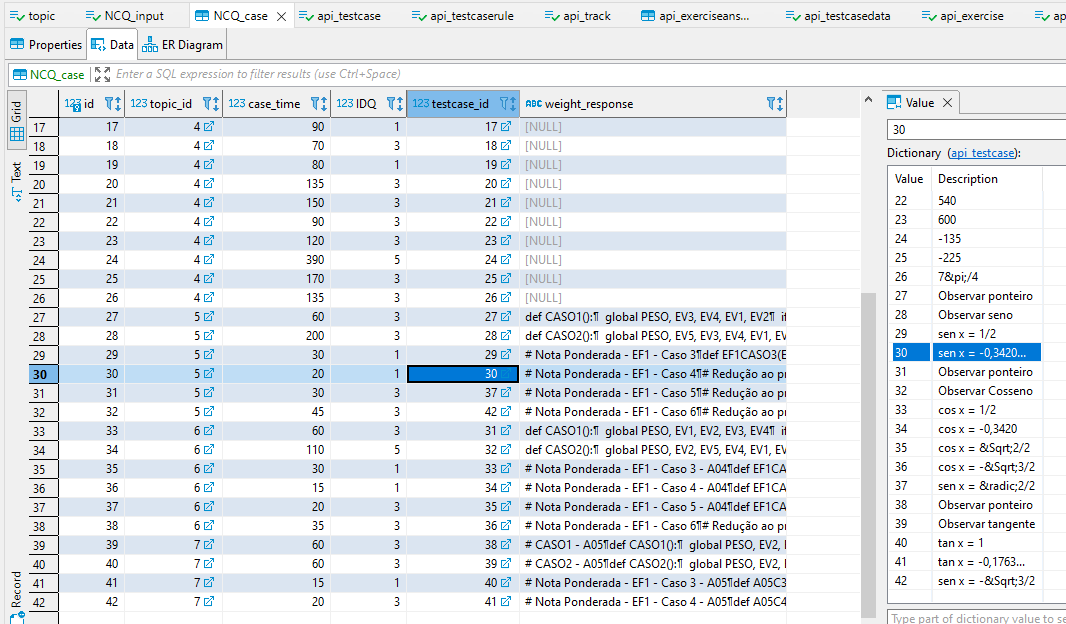
\includegraphics[width=1\linewidth]{chapters/proposedMethod/tools/NCQ_case.png}
	\caption{Parâmetros do NCQ - Casos de Teste}
	\label{fig:NCQ_case}
\end{figure}

De acordo com os modelos apresentados anteriormente, as métricas que exigem um maior detalhamento são (i) `Nota Ponderada': cuja associação entre entradas e pesos foi feita por meio da ferramenta de programação em blocos implementada para este trabalho (Figura~\ref{fig:CASO1NPEF1}) que converte os blocos criados para um código-fonte em \textit{python} e cujos parâmetros definidos podem ser encontrados nos Apêndices~\ref{Chap:AppendixAnaliticos}, \ref{Chap:AppendixAnaliticosA02},  \ref{Chap:AppendixAnaliticosA03},  \ref{Chap:AppendixAnaliticosA04} e  \ref{Chap:AppendixAnaliticosA05}; e, (ii) `Nível de Compreensão da Questão', cujos parâmetros foram definidos através da população das tabelas \textit{$NCQ\_input$} e \textit{$NCQ\_case$} definidas no banco de dados SQL que armazena os dados do objeto tangível (Figuras~\ref{fig:NCQ_entradas} e~\ref{fig:NCQ_case}).

Assim, as subseções a seguir apresentam possibilidades de cálculo das métricas tomando como base os parâmetros que podem ser especificados para cada uma delas. É importante notar que a escolha da base de cálculo (i.e.: por entrada, caso de teste ou considerando os possíveis agrupamentos indicados na construção do OTA) impacta no resultado final das notas obtidas pelos estudantes, sendo um critério a ser levado em consideração pelo profissional que deseja avaliar o processo de aprendizagem.

\subsubsection{Exercício 1 - Quadrantes}\label{subsubsec:F3A1}

O Exercício 1, cujos parâmetros estão definidos no Apêndice~\ref{Chap:AppendixB}, consiste em uma instanciação do objeto tangível Quadro Trigonométrico que adapta a primeira questão do exercício de fixação tradicional (disponível na Seção~\ref{section:atividade2_fixação}), de modo que os ponteiros do objeto de tangível aprendizagem implementado sejam utilizados no processo de descoberta dos limites iniciais e finais de cada um dos quadrantes do círculo trigonométrico, onde a Interface Física A01 (ver Seção~\ref{subsection:atividade3_A01}) contém apenas uma circunferência orientada de raio 1.

\begin{figure}[htb]
	\centering
	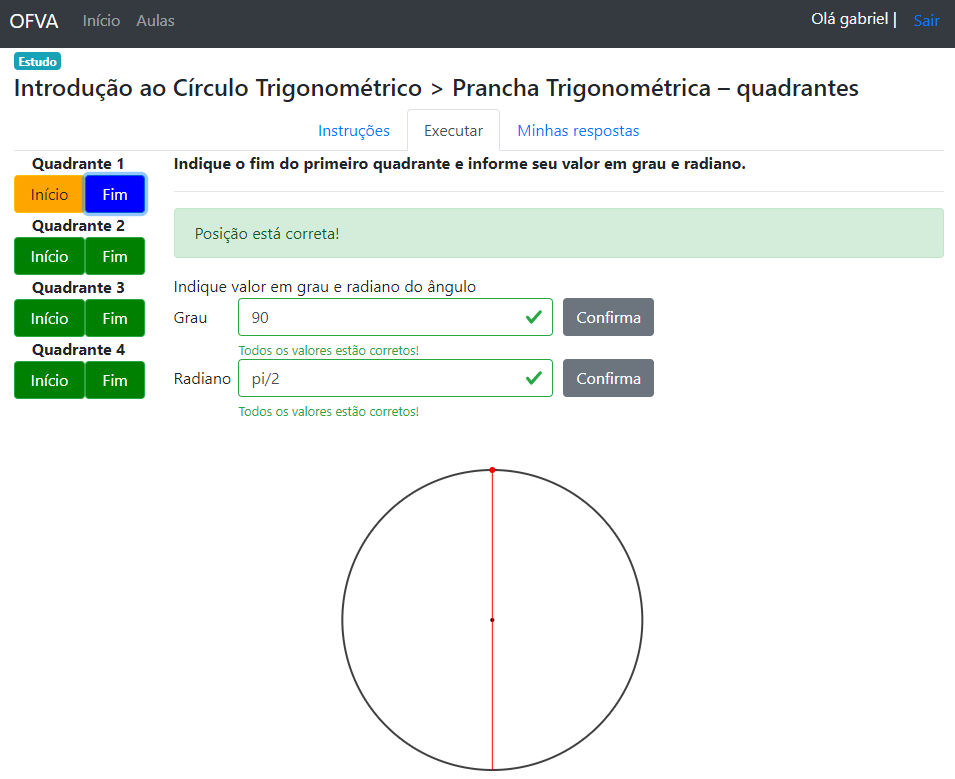
\includegraphics[width=0.8\linewidth]{chapters/results/Fase 3/E1_Virtual_2.png}
	\caption{Exercício 1 - Quadrantes}
	\label{fig:E1}
\end{figure}

A Figura~\ref{fig:E1} mostra o estudante respondendo a segunda questão do exercício, onde é possível observar que há \textit{feedbacks} que auxiliam no processo de encontrar o ângulo correto a partir da posição do ponteiro da interface física do objeto. Além disso, pode-se notar que, para cada informação inserida pelo estudante, há uma resposta do sistema que indica o que fazer para chegar a resposta correta, por exemplo, se o ponteiro deve ser movido no sentido horário ou anti-horário, ou se os valores inseridos nos campos `Grau' ou `Radiano' estão corretos ou deveriam ser maiores/menores (ver Tabela `Entradas e Saídas' no Apêndice~\ref{Chap:AppendixB}). 

Além disso, na Figura~\ref{fig:E1} também é possível observar uma coloração diferenciada nas questões, onde a cor `azul' indica o caso de teste que está selecionado, a cor `amarelo' significa que falta complementar algum item e, `verde' simboliza que todas as respostas do caso de teste estão corretas. É importante ressaltar que os \textit{feedbacks} adicionados tem o objetivo de colaborar com a construção do conhecimento por parte dos estudantes de modo que sejam um auxílio para que ele entenda a lógica por trás do ciclo trigonométrico, bem como os conceitos matemáticos envolvidos, de modo que cada um dos exercícios colabora com a construção de um aprendizado específico, sendo este primeiro exercício uma interação com as noções de quadrante, ângulo reto, além do fortalecimento do aprendizado sobre `regra de três' para conversão entre graus e radianos.

\subsubsection*{Nota Tradicional ($NT$)}
Considerando o modelo de processos apresentado na Figura~\ref{fig:bpmn_metricas_NT}, com relação à nota tradicional, o cálculo dessa métrica pode ser baseado `nas entradas' ou `nos casos de teste', caso seja baseado nas entradas, as métricas serão calculadas de modo proporcional, o que significa que será calculada a média das respostas de uma mesma entrada para todos os casos de teste, o que permite a verificação da aprendizagem a partir de um ponto de interação específico (e que pode corresponder a um tópico de estudo específico). 

Além disso, a Figura~\ref{fig:bpmn_metricas} que apresenta o modelo geral para aplicação das métricas em objetos tangíveis, o processo `Definir 'agrupamentos' como critério de cálculo' indica que a métrica também pode ser calculada levando em consideração que os casos de teste estão agrupados em conjuntos menores.

Assim, na análise dos dados de nota tradicional desta seção, quando considerada a existência de agrupamentos, o que significa que os casos de teste estão organizados em subconjuntos conforme a Tabela~\ref{tab:F3_Agrupamentos} extraída do Apêndice~\ref{Chap:AppendixB}, todas as respostas dada por um estudante para todos os casos de teste de um agrupamento devem estar corretas para que este agrupamento esteja correto, onde a nota tradicional da entrada é calculada como a média das respostas de cada agrupamento.
%Para a análise dos dados de nota tradicional desta seção, será considerada a existência de agrupamentos, o que significa que os casos de teste estão organizados em subconjuntos conforme a Tabela~\ref{tab:F3_Agrupamentos} extraída do Apêndice~\ref{Chap:AppendixB}, de modo que todas as respostas dada por um estudante para todos os casos de teste de um agrupamento devem estar corretas para que este agrupamento esteja correto, onde a nota tradicional é calculada como a média das respostas de cada agrupamento.

\begin{table}[htbp]
	\centering
	\caption{Exercício 1 - Agrupamentos}
	\begin{tabular}{|c|c|}
		\hline
		\cellcolor[HTML]{C0C0C0}\textbf{AGRUPAR CASOS DE TESTE?} & SIM \\ \hline
		\cellcolor[HTML]{DEDEDE}\textbf{ID GRUPO} & \cellcolor[HTML]{DEDEDE}1\\ \hline
		\textbf{RÓTULO} & QUADRANTE 1 \\ \hline
		\textbf{AGRUPAMENTO} & \{1,2\}\\ \hline
		\cellcolor[HTML]{DEDEDE}\textbf{ID GRUPO} & \cellcolor[HTML]{DEDEDE}2\\ \hline
		\textbf{RÓTULO} & QUADRANTE 2 \\ \hline
		\textbf{AGRUPAMENTO} & \{3,4\}\\ \hline
		\cellcolor[HTML]{DEDEDE}\textbf{ID GRUPO} & \cellcolor[HTML]{DEDEDE}3\\ \hline
		\textbf{RÓTULO} & QUADRANTE 3 \\ \hline
		\textbf{AGRUPAMENTO} & \{5,6\}\\ \hline
		\cellcolor[HTML]{DEDEDE}\textbf{ID GRUPO} & \cellcolor[HTML]{DEDEDE}4\\ \hline
		\textbf{RÓTULO} & QUADRANTE 4 \\ \hline
		\textbf{AGRUPAMENTO} & \{7,8\}\\ \hline	
	\end{tabular}
	\label{tab:F3_Agrupamentos}
\end{table}

\textbf{$NT$: Cálculo por Entrada}

A Tabela~\ref{tab:F3_NT_entradas} apresenta a nota tradicional baseada nas entradas, de modo que no lado esquerdo da tabela pode-se observar as notas tradicionais obtidas pelo Grupo B considerando que os casos de teste estavam agrupados, enquanto no lado direito da mesma tabela estão as notas relativas às entradas desconsiderando os agrupamentos. 

\begin{table}[htbp]
	\centering
	\caption{Nota Tradicional - Cálculo por Entrada com método proporcional}
	\begin{tabular}{|
			>{\columncolor[HTML]{EFEFEF}}c cccc
			>{\columncolor[HTML]{EFEFEF}}c 
			>{\columncolor[HTML]{EFEFEF}}c 
			>{\columncolor[HTML]{EFEFEF}}c 
			>{\columncolor[HTML]{EFEFEF}}c |}
		\hline
%		\multicolumn{9}{|c|}{\cellcolor[HTML]{C0C0C0}\textbf{NOTA   TRADICIONAL}} \\ \hline
		\multicolumn{1}{|c|}{\cellcolor[HTML]{EFEFEF}\textbf{Agrupamento}} & \multicolumn{4}{c|}{Sim} & \multicolumn{4}{c|}{\cellcolor[HTML]{EFEFEF}Não} \\ \hline
		\multicolumn{1}{|c|}{\cellcolor[HTML]{C0C0C0}\textbf{Participante}} & \multicolumn{1}{c|}{\cellcolor[HTML]{C0C0C0}\textbf{EF1}} & \multicolumn{1}{c|}{\cellcolor[HTML]{C0C0C0}\textbf{EV1}} & \multicolumn{1}{c|}{\cellcolor[HTML]{C0C0C0}\textbf{EV2}} & \multicolumn{1}{c|}{\cellcolor[HTML]{C0C0C0}\textbf{Média}} & \multicolumn{1}{c|}{\cellcolor[HTML]{C0C0C0}\textbf{EF1}} & \multicolumn{1}{c|}{\cellcolor[HTML]{C0C0C0}\textbf{EV1}} & \multicolumn{1}{c|}{\cellcolor[HTML]{C0C0C0}\textbf{EV2}} & \cellcolor[HTML]{C0C0C0}\textbf{Média} \\ \hline
		\multicolumn{1}{|c|}{\cellcolor[HTML]{F2F2F2}\textbf{B02}} & \multicolumn{1}{c|}{10.00} & \multicolumn{1}{c|}{10.00} & \multicolumn{1}{c|}{7.50} & \multicolumn{1}{c|}{9.167} & \multicolumn{1}{c|}{\cellcolor[HTML]{F2F2F2}10.00} & \multicolumn{1}{c|}{\cellcolor[HTML]{F2F2F2}10.00} & \multicolumn{1}{c|}{\cellcolor[HTML]{F2F2F2}8.75} & 9.583 \\ \hline
		\multicolumn{1}{|c|}{\cellcolor[HTML]{F2F2F2}\textbf{B03}} & \multicolumn{1}{c|}{10.00} & \multicolumn{1}{c|}{10.00} & \multicolumn{1}{c|}{10.00} & \multicolumn{1}{c|}{10.000} & \multicolumn{1}{c|}{\cellcolor[HTML]{F2F2F2}10.00} & \multicolumn{1}{c|}{\cellcolor[HTML]{F2F2F2}10.00} & \multicolumn{1}{c|}{\cellcolor[HTML]{F2F2F2}10.00} & 10.000 \\ \hline
		\multicolumn{1}{|c|}{\cellcolor[HTML]{F2F2F2}\textbf{B04}} & \multicolumn{1}{c|}{7.50} & \multicolumn{1}{c|}{10.00} & \multicolumn{1}{c|}{10.00} & \multicolumn{1}{c|}{9.167} & \multicolumn{1}{c|}{\cellcolor[HTML]{F2F2F2}8.75} & \multicolumn{1}{c|}{\cellcolor[HTML]{F2F2F2}10.00} & \multicolumn{1}{c|}{\cellcolor[HTML]{F2F2F2}10.00} & 9.583 \\ \hline
		\multicolumn{1}{|c|}{\cellcolor[HTML]{F2F2F2}\textbf{B05}} & \multicolumn{1}{c|}{7.50} & \multicolumn{1}{c|}{10.00} & \multicolumn{1}{c|}{10.00} & \multicolumn{1}{c|}{9.167} & \multicolumn{1}{c|}{\cellcolor[HTML]{F2F2F2}8.75} & \multicolumn{1}{c|}{\cellcolor[HTML]{F2F2F2}10.00} & \multicolumn{1}{c|}{\cellcolor[HTML]{F2F2F2}10.00} & 9.583 \\ \hline
		\multicolumn{1}{|c|}{\cellcolor[HTML]{F2F2F2}\textbf{B06}} & \multicolumn{1}{c|}{10.00} & \multicolumn{1}{c|}{10.00} & \multicolumn{1}{c|}{10.00} & \multicolumn{1}{c|}{10.000} & \multicolumn{1}{c|}{\cellcolor[HTML]{F2F2F2}10.00} & \multicolumn{1}{c|}{\cellcolor[HTML]{F2F2F2}10.00} & \multicolumn{1}{c|}{\cellcolor[HTML]{F2F2F2}10.00} & 10.000 \\ \hline
%		\multicolumn{1}{|c|}{\cellcolor[HTML]{F2F2F2}\textbf{B07}} & \multicolumn{1}{c|}{2.50} & \multicolumn{1}{c|}{0.00} & \multicolumn{1}{c|}{0.00} & \multicolumn{1}{c|}{0.833} & \multicolumn{1}{c|}{\cellcolor[HTML]{F2F2F2}1.25} & \multicolumn{1}{c|}{\cellcolor[HTML]{F2F2F2}1.25} & \multicolumn{1}{c|}{\cellcolor[HTML]{F2F2F2}1.25} & 1.250 \\ \hline
		\multicolumn{1}{|c|}{\cellcolor[HTML]{F2F2F2}\textbf{B08}} & \multicolumn{1}{c|}{10.00} & \multicolumn{1}{c|}{10.00} & \multicolumn{1}{c|}{10.00} & \multicolumn{1}{c|}{10.000} & \multicolumn{1}{c|}{\cellcolor[HTML]{F2F2F2}10.00} & \multicolumn{1}{c|}{\cellcolor[HTML]{F2F2F2}10.00} & \multicolumn{1}{c|}{\cellcolor[HTML]{F2F2F2}10.00} & 10.000 \\ \hline
		\multicolumn{1}{|c|}{\cellcolor[HTML]{F2F2F2}\textbf{B09}} & \multicolumn{1}{c|}{10.00} & \multicolumn{1}{c|}{10.00} & \multicolumn{1}{c|}{10.00} & \multicolumn{1}{c|}{10.000} & \multicolumn{1}{c|}{\cellcolor[HTML]{F2F2F2}10.00} & \multicolumn{1}{c|}{\cellcolor[HTML]{F2F2F2}10.00} & \multicolumn{1}{c|}{\cellcolor[HTML]{F2F2F2}10.00} & 10.000 \\ \hline
		\multicolumn{1}{|c|}{\cellcolor[HTML]{F2F2F2}\textbf{B10}} & \multicolumn{1}{c|}{10.00} & \multicolumn{1}{c|}{10.00} & \multicolumn{1}{c|}{10.00} & \multicolumn{1}{c|}{10.000} & \multicolumn{1}{c|}{\cellcolor[HTML]{F2F2F2}10.00} & \multicolumn{1}{c|}{\cellcolor[HTML]{F2F2F2}10.00} & \multicolumn{1}{c|}{\cellcolor[HTML]{F2F2F2}10.00} & 10.000 \\ \hline
		\multicolumn{1}{|c|}{\cellcolor[HTML]{D0CECE}\textbf{Média}} & \multicolumn{1}{c|}{\cellcolor[HTML]{D0CECE}9.38} & \multicolumn{1}{c|}{\cellcolor[HTML]{D0CECE}10.00} & \multicolumn{1}{c|}{\cellcolor[HTML]{D0CECE}9.69} & \multicolumn{1}{c|}{\cellcolor[HTML]{D0CECE}9.69} & \multicolumn{1}{c|}{\cellcolor[HTML]{D0CECE}9.69} & \multicolumn{1}{c|}{\cellcolor[HTML]{D0CECE}10.00} & \multicolumn{1}{c|}{\cellcolor[HTML]{D0CECE}9.84} & \cellcolor[HTML]{D0CECE}9.84 \\ \hline
	\end{tabular}
	\label{tab:F3_NT_entradas}
\end{table}

É importante notar que optar por uma ou outra forma de calcular impacta no resultado final, de modo que as notas calculadas sem os agrupamentos são maiores do que as provenientes de agrupamento. Entretanto, é preciso levar em consideração o objetivo da avaliação da aprendizagem, assim, para a atividade em questão, os agrupamentos consideram o início e o fim de cada quadrante como uma mesma unidade avaliativa, de modo que a nota corresponde ao estudante identificar corretamente os limites de um quadrante, enquanto o cálculo sem agrupamento corresponde tão somente aos ângulos isolados, de modo que sua nota implica em verificar se o estudante identifica corretamente cada ângulo solicitado.

De todo modo, independentemente da opção escolhida, é possível notar que o participante $B02$ teve mais dificuldade com a entrada $EV2$, o que significa uma maior dificuldade com ângulos em radiano, assim como os participantes $B04$ e $B05$ tiveram maior dificuldade com a localização do ângulo no círculo trigonométrico, uma vez que o ponteiro físico corresponde a entrada $EF1$, cujo valor foi mais baixo para este participantes. 

Como o objetivo do objeto de aprendizagem é que o estudante chegue ao fim da atividade tendo construído e identificado os quadrantes do círculo trigonométrico, é esperado que todos os valores da nota tradicional sejam iguais a $10.00$, de modo que quando um estudante não alcança esse valor, pode ser um indicativo de que não terminou a atividade ou teve alguma dificuldade. 

Por fim, ao observar a média das notas tradicionais de cada entrada em ambos os modos de cálculo (com ou sem agrupamento), é possível notar com quais entradas os estudantes tiveram mais dificuldade, de modo que estas entradas podem também estar associadas a tópicos de estudo. Assim, as entradas $EF1$ e $EV2$ foram as que apresentaram menor valor de nota tradicional, de modo que pode-se considerar que a dificuldade maior se deu tanto para identificar o ângulo no objeto físico quanto para converter os valores para radianos.

\textbf{$NT$: Cálculo por Caso de Teste}

A Tabela~\ref{tab:F3_NT_casos} apresenta quatro possibilidades de cálculo da nota tradicional com objetos tangíveis, onde, além de levar em consideração se os dados estão ou não agrupados, o cálculo é feito através de uma correção binária (se todas as entradas de um caso estiverem corretas, então, o caso está correto) ou proporcional (média das entradas de cada caso).

\begin{table}[htbp]
	\centering
	\caption{Nota Tradicional - Cálculo por Casos de Teste}
\begin{tabular}{|
		>{\columncolor[HTML]{F2F2F2}}c |cc|
		>{\columncolor[HTML]{F2F2F2}}c 
		>{\columncolor[HTML]{F2F2F2}}c |}
	\hline
	\cellcolor[HTML]{D0CECE}\textbf{Modo} & \multicolumn{2}{c|}{\cellcolor[HTML]{D0CECE}\textbf{Binário}} & \multicolumn{2}{c|}{\cellcolor[HTML]{D0CECE}\textbf{Proporcional}} \\ \hline
	\textbf{Agrupamento} & \multicolumn{1}{c|}{Sim} & Não & \multicolumn{1}{c|}{\cellcolor[HTML]{F2F2F2}Sim} & Não \\ \hline
%	\cellcolor[HTML]{D0CECE}\textbf{Participante} & \multicolumn{1}{c|}{\cellcolor[HTML]{D0CECE}\textbf{NT}} & \cellcolor[HTML]{D0CECE}\textbf{NT} & \multicolumn{1}{c|}{\cellcolor[HTML]{D0CECE}\textbf{}} & \cellcolor[HTML]{D0CECE}\textbf{} \\ \hline
	\textbf{B02} & \multicolumn{1}{c|}{7.50} & 8.75 & \multicolumn{1}{c|}{\cellcolor[HTML]{F2F2F2}9.17} & 9.58 \\ \hline
	\textbf{B03} & \multicolumn{1}{c|}{10.00} & 10.00 & \multicolumn{1}{c|}{\cellcolor[HTML]{F2F2F2}10.00} & 10.00 \\ \hline
	\textbf{B04} & \multicolumn{1}{c|}{7.50} & 8.75 & \multicolumn{1}{c|}{\cellcolor[HTML]{F2F2F2}9.17} & 9.58 \\ \hline
	\textbf{B05} & \multicolumn{1}{c|}{7.50} & 8.75 & \multicolumn{1}{c|}{\cellcolor[HTML]{F2F2F2}9.17} & 9.58 \\ \hline
	\textbf{B06} & \multicolumn{1}{c|}{10.00} & 10.00 & \multicolumn{1}{c|}{\cellcolor[HTML]{F2F2F2}10.00} & 10.00 \\ \hline
%	\textbf{B07} & \multicolumn{1}{c|}{0.00} & 1.25 & \multicolumn{1}{c|}{\cellcolor[HTML]{F2F2F2}0.83} & 1.250 \\ \hline
	\textbf{B08} & \multicolumn{1}{c|}{10.00} & 10.00 & \multicolumn{1}{c|}{\cellcolor[HTML]{F2F2F2}10.00} & 10.00 \\ \hline
	\textbf{B09} & \multicolumn{1}{c|}{10.00} & 10.00 & \multicolumn{1}{c|}{\cellcolor[HTML]{F2F2F2}10.00} & 10.00 \\ \hline
	\textbf{B10} & \multicolumn{1}{c|}{10.00} & 10.00 & \multicolumn{1}{c|}{\cellcolor[HTML]{F2F2F2}10.00} & 10.00 \\ \hline
	\cellcolor[HTML]{D0CECE}\textbf{Média} & \multicolumn{1}{c|}{\cellcolor[HTML]{D0CECE}9.06} & \cellcolor[HTML]{D0CECE}9.53 & \multicolumn{1}{c|}{\cellcolor[HTML]{D0CECE}9.69} & \cellcolor[HTML]{D0CECE}9.84 \\ \hline
\end{tabular}
	\label{tab:F3_NT_casos}
\end{table}

Neste modo de cálculo, cada caso de teste funciona como uma questão, onde as entradas são agrupadas por caso, tendo uma saída diferente se o tipo de correção for binária ou proporcional. Assim, a partir da Tabela~\ref{tab:F3_NT_casos}, pode-se observar que os alunos com mais dificuldade foram $B2$, $B4$ e $B5$, uma vez que possuem nota abaixo de $10.00$. 

Assim como a abordagem de cálculo `por entrada', a escolha de algum dos modos de calcular a nota tradicional depende dos critérios avaliativos adotados, por exemplo, a escolha por um modo de cálculo binário atende uma perspectiva de que o estudante aprendeu somente se acertou completamente as questões (casos de teste) e a escolha por um modo proporcional leva em consideração que a aprendizagem é um processo e, assim, é importante considerar o conjunto das respostas para se fazer um acompanhamento.

\textbf{Nota Ponderada ($NP$)}

De acordo com o diagrama BPMN das métricas (Figura~\ref{fig:bpmn_metricas}), após a definição dos parâmetros da nota tradicional, são definidos os parâmetros da nota ponderada, de modo que o subprocesso da Figura~\ref{fig:bpmn_metricas_NP} apresenta as ações necessárias para essa definição de parâmetros, cujo resultado é a associação dos pesos e das respostas esperadas às entradas dos casos de teste de um objeto tangível. 

Com relação ao Exercício 1, estas ações geraram os dados do Apêndice~\ref{Chap:AppendixAnaliticos} e do banco de dados apresentado na Figura~\ref{fig:NCQ_case} de modo que, no recorte da Tabela~\ref{tab:F3_NP_Exemplo}, é possível observar um exemplo da associação entre a entrada $EV2$, os pesos das possíveis respostas e o Caso de Teste 1, onde a ferramenta de programação em blocos adaptada gerou um código-fonte em \textit{python} a ser utilizado para efetiva atribuição dos pesos às respostas do estudante pelo módulo Analíticos.

\begin{table}[htbp]
	\centering
	\caption{Nota Ponderada - Associação entre pesos, entradas e casos de teste}
	\begin{xltabular}{\textwidth}{|l|X|X|}
		\hline
		\endfirsthead
		
		\hline \multicolumn{3}{|c|}{continuação da página anterior} \\ \hline
		\endhead
		
		\hline \multicolumn{3}{|r|}{Continua na próxima página} \\ \hline
		\endfoot
		
		\hline
		\endlastfoot
		
		\multicolumn{3}{|c|}{\cellcolor[HTML]{C0C0C0}\textbf{CASO DE TESTE 1}} \\ \hline
			
		%EV2
		\multicolumn{3}{|c|}{\cellcolor[HTML]{DEDEDE}\textbf{Nota Ponderada - EV2}} \\ \hline
		\multicolumn{3}{|c|}{\textbf{Blocos}} \\ \hline
		\multicolumn{3}{|l|}{\begin{tabular}[c]{@{}l@{}} \\ 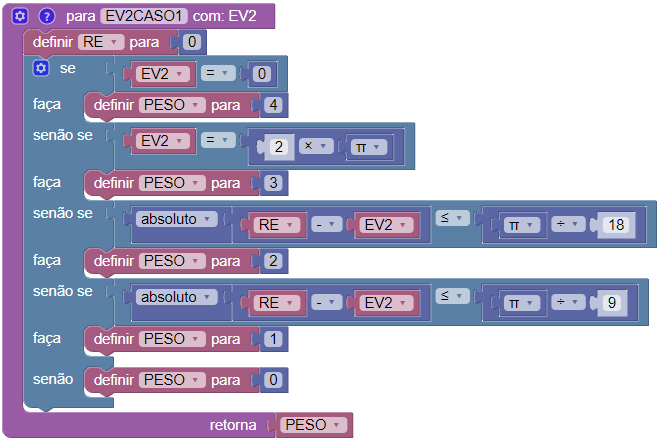
\includegraphics[width=0.9\linewidth]{chapters/appendixAnalytics/CASO1NPEV2.png}  \end{tabular}
		} \\ \hline
		\multicolumn{3}{|c|}{\textbf{Python gerado}} \\ \hline
		\multicolumn{3}{|l|}{ \begin{tabular}[c]{@{}l@{}}import math\\ \# Nota Ponderada - Caso 1\\  def EV2CASO1(EV2):\\ \quad	global RE, PESO\\ \quad	RE = 0\\ \quad if EV2 == 0:\\ \quad \quad PESO = 4\\ \quad elif EV2 == 2 * math.pi:\\ \quad \quad	PESO = 3\\ \quad elif math.fabs(RE - EV2) <= math.pi / 18:\\ \quad \quad	PESO = 2\\ \quad	elif math.fabs(RE - EV2) <= math.pi / 9:\\ \quad \quad	PESO = 1\\ \quad	else:\\ \quad \quad		PESO = 0\\ \quad return PESO \end{tabular} }\\ \hline
		
	\end{xltabular}
	\label{tab:F3_NP_Exemplo}
\end{table}

\textbf{$NP$: Cálculo por Entrada}

Como explicado na Seção~\ref{sec:nota-ponderada}, a nota ponderada considera o quão próximo a resposta dada pelo estudante está do correto, de modo que a Tabela~\ref{tab:F3_NP_entradas} apresenta os valores de $NP$ calculados com base no modo `por entrada', onde a nota ponderada é calculada a partir do peso médio, isto é, a média dos pesos de todas as respostas dadas pelo estudante ao manipular o objeto tangível a partir de uma determinada entrada (física ou virtual). Assim, esses pesos médios são utilizados para o cálculo da métrica segundo a Equação~\ref{eq:NP}.

\begin{table}[htbp]
	\centering
	\caption{Nota Ponderada - Cálculo por Entrada}
\begin{tabular}{|
		>{\columncolor[HTML]{EFEFEF}}c cccc
		>{\columncolor[HTML]{EFEFEF}}c 
		>{\columncolor[HTML]{EFEFEF}}c 
		>{\columncolor[HTML]{EFEFEF}}c 
		>{\columncolor[HTML]{EFEFEF}}c |}
	\hline
%	\multicolumn{9}{|c|}{\cellcolor[HTML]{D0CECE}\textbf{NOTA   PONDERADA}} \\ \hline
	\multicolumn{1}{|c|}{\cellcolor[HTML]{EFEFEF}\textbf{Agrupamento}} & \multicolumn{4}{c|}{Sim} & \multicolumn{4}{c|}{\cellcolor[HTML]{EFEFEF}Não} \\ \hline
	\multicolumn{1}{|c|}{\cellcolor[HTML]{D0CECE}\textbf{Participante}} & \multicolumn{1}{c|}{\cellcolor[HTML]{D0CECE}\textbf{EF1}} & \multicolumn{1}{c|}{\cellcolor[HTML]{D0CECE}\textbf{EV1}} & \multicolumn{1}{c|}{\cellcolor[HTML]{D0CECE}\textbf{EV2}} & \multicolumn{1}{c|}{\cellcolor[HTML]{D0CECE}\textbf{Média}} & \multicolumn{1}{c|}{\cellcolor[HTML]{D0CECE}\textbf{EF1}} & \multicolumn{1}{c|}{\cellcolor[HTML]{D0CECE}\textbf{EV1}} & \multicolumn{1}{c|}{\cellcolor[HTML]{D0CECE}\textbf{EV2}} & \cellcolor[HTML]{D0CECE}\textbf{Média} \\ \hline
	\multicolumn{1}{|c|}{\cellcolor[HTML]{EFEFEF}\textbf{B02}} & \multicolumn{1}{c|}{9.58} & \multicolumn{1}{c|}{10.00} & \multicolumn{1}{c|}{8.75} & \multicolumn{1}{c|}{9.444} & \multicolumn{1}{c|}{\cellcolor[HTML]{EFEFEF}9.58} & \multicolumn{1}{c|}{\cellcolor[HTML]{EFEFEF}10.00} & \multicolumn{1}{c|}{\cellcolor[HTML]{EFEFEF}8.75} & 9.444 \\ \hline
	\multicolumn{1}{|c|}{\cellcolor[HTML]{EFEFEF}\textbf{B03}} & \multicolumn{1}{c|}{8.54} & \multicolumn{1}{c|}{9.38} & \multicolumn{1}{c|}{10.00} & \multicolumn{1}{c|}{9.306} & \multicolumn{1}{c|}{\cellcolor[HTML]{EFEFEF}8.54} & \multicolumn{1}{c|}{\cellcolor[HTML]{EFEFEF}9.38} & \multicolumn{1}{c|}{\cellcolor[HTML]{EFEFEF}10.00} & 9.306 \\ \hline
	\multicolumn{1}{|c|}{\cellcolor[HTML]{EFEFEF}\textbf{B04}} & \multicolumn{1}{c|}{4.95} & \multicolumn{1}{c|}{9.38} & \multicolumn{1}{c|}{9.00} & \multicolumn{1}{c|}{7.775} & \multicolumn{1}{c|}{\cellcolor[HTML]{EFEFEF}4.96} & \multicolumn{1}{c|}{\cellcolor[HTML]{EFEFEF}9.38} & \multicolumn{1}{c|}{\cellcolor[HTML]{EFEFEF}9.00} & 7.777 \\ \hline
	\multicolumn{1}{|c|}{\cellcolor[HTML]{EFEFEF}\textbf{B05}} & \multicolumn{1}{c|}{8.54} & \multicolumn{1}{c|}{9.38} & \multicolumn{1}{c|}{7.09} & \multicolumn{1}{c|}{8.336} & \multicolumn{1}{c|}{\cellcolor[HTML]{EFEFEF}8.54} & \multicolumn{1}{c|}{\cellcolor[HTML]{EFEFEF}9.38} & \multicolumn{1}{c|}{\cellcolor[HTML]{EFEFEF}7.09} & 8.336 \\ \hline
	\multicolumn{1}{|c|}{\cellcolor[HTML]{EFEFEF}\textbf{B06}} & \multicolumn{1}{c|}{8.54} & \multicolumn{1}{c|}{8.75} & \multicolumn{1}{c|}{10.00} & \multicolumn{1}{c|}{9.097} & \multicolumn{1}{c|}{\cellcolor[HTML]{EFEFEF}8.54} & \multicolumn{1}{c|}{\cellcolor[HTML]{EFEFEF}8.75} & \multicolumn{1}{c|}{\cellcolor[HTML]{EFEFEF}10.00} & 9.097 \\ \hline
%	\multicolumn{1}{|c|}{\cellcolor[HTML]{EFEFEF}\textbf{B07}} & \multicolumn{1}{c|}{} & \multicolumn{1}{c|}{} & \multicolumn{1}{c|}{} & \multicolumn{1}{c|}{} & \multicolumn{1}{c|}{\cellcolor[HTML]{EFEFEF}} & \multicolumn{1}{c|}{\cellcolor[HTML]{EFEFEF}} & \multicolumn{1}{c|}{\cellcolor[HTML]{EFEFEF}} &  \\ \hline
	\multicolumn{1}{|c|}{\cellcolor[HTML]{EFEFEF}\textbf{B08}} & \multicolumn{1}{c|}{8.85} & \multicolumn{1}{c|}{10.00} & \multicolumn{1}{c|}{9.38} & \multicolumn{1}{c|}{9.410} & \multicolumn{1}{c|}{\cellcolor[HTML]{EFEFEF}8.85} & \multicolumn{1}{c|}{\cellcolor[HTML]{EFEFEF}10.00} & \multicolumn{1}{c|}{\cellcolor[HTML]{EFEFEF}9.38} & 9.410 \\ \hline
	\multicolumn{1}{|c|}{\cellcolor[HTML]{EFEFEF}\textbf{B09}} & \multicolumn{1}{c|}{9.51} & \multicolumn{1}{c|}{9.38} & \multicolumn{1}{c|}{8.57} & \multicolumn{1}{c|}{9.151} & \multicolumn{1}{c|}{\cellcolor[HTML]{EFEFEF}9.51} & \multicolumn{1}{c|}{\cellcolor[HTML]{EFEFEF}9.38} & \multicolumn{1}{c|}{\cellcolor[HTML]{EFEFEF}8.57} & 9.151 \\ \hline
	\multicolumn{1}{|c|}{\cellcolor[HTML]{EFEFEF}\textbf{B10}} & \multicolumn{1}{c|}{10.00} & \multicolumn{1}{c|}{10.00} & \multicolumn{1}{c|}{7.50} & \multicolumn{1}{c|}{9.167} & \multicolumn{1}{c|}{\cellcolor[HTML]{EFEFEF}10.00} & \multicolumn{1}{c|}{\cellcolor[HTML]{EFEFEF}10.00} & \multicolumn{1}{c|}{\cellcolor[HTML]{EFEFEF}7.50} & 9.167 \\ \hline
	\multicolumn{1}{|c|}{\cellcolor[HTML]{D0CECE}\textbf{Média}} & \multicolumn{1}{c|}{\cellcolor[HTML]{D0CECE}8.56} & \multicolumn{1}{c|}{\cellcolor[HTML]{D0CECE}9.53} & \multicolumn{1}{c|}{\cellcolor[HTML]{D0CECE}8.79} & \multicolumn{1}{c|}{\cellcolor[HTML]{D0CECE}8.96} & \multicolumn{1}{c|}{\cellcolor[HTML]{D0CECE}8.57} & \multicolumn{1}{c|}{\cellcolor[HTML]{D0CECE}9.53} & \multicolumn{1}{c|}{\cellcolor[HTML]{D0CECE}8.79} & \cellcolor[HTML]{D0CECE}8.96 \\ \hline
\end{tabular}
	\label{tab:F3_NP_entradas}
\end{table}

É interessante notar na Tabela~\ref{tab:F3_NP_entradas} que, com ou sem agrupamento, diferentemente da nota tradicional, as notas ponderadas dos participantes para as diversas entradas é sempre a mesma, o que pode significar uma maior estabilidade desta métrica no que diz respeito ao acompanhamento do processo de aprendizagem, uma vez que a nota tradicional tende a $10.00$ e somente se afasta desse valor quando o estudante não concluiu a atividade.

Com relação à entrada $EF1$, é possível notar uma maior variabilidade nas notas do que na métrica tradicional e, embora na $NT$, os participantes $B4$ e $B5$ tenham sido apontados dentre os indivíduos com maior dificuldade, na $NP$, enquanto o percurso feito por $B5$ está na média do grupo, $B4$ foi confirmado como o participante com desempenho mais baixo.

Tendo em vista $EV1$, $B06$ foi o participante com a menor nota ($8.75$), embora ainda acima da média do grupo ($9.53$). E, com relação à $EV2$, que prevê conversão entre graus e radianos, os participantes $B04$ e $B10$ obtiveram as menores notas ponderadas do grupo, sendo $7.09$ e $7.50$, respectivamente.

Por fim, observando a média das entradas, os participantes com menor pontuação são $B04$ e $B05$, cujas notas ($7.775$ e $8.336$) estão abaixo da média do grupo ($8.96$), necessitando de maior atenção por parte do professor.

\textbf{$NP$: Cálculo por Caso de Teste}

Para o cálculo da nota ponderada por casos de teste, o peso final do caso é a média dos pesos médios de todas as entradas do caso, de modo que todo o percurso do estudante na construção do conhecimento acerca dos quadrantes do círculo trigonométrico é levado em consideração. 

É importante notar que, assim como ocorreu na Tabela~\ref{tab:F3_NP_entradas} para cada entrada, as colunas com e sem agrupamento da Tabela~\ref{tab:F3_NP_casos} apresentam os mesmos valores para cada participante, de modo que, para este modo de cálculo das métricas, é indiferente se a métrica é calculada com base nestes agrupamentos (o que confirma a decisão deste parâmetro não ser considerado no subprocesso da Nota Tradicional da Figura~\ref{fig:bpmn_metricas_NP}).

\begin{table}[htbp]
	\centering
	\caption{Nota Ponderada - Cálculo por Caso de Teste (com e sem agrupamento)}
	\begin{tabular}{|
			>{\columncolor[HTML]{E0E0E0}}c |c|
			>{\columncolor[HTML]{E0E0E0}}c |}
		\hline
		\cellcolor[HTML]{C0C0C0}\textbf{Agrupamento} & Sim & Não \\ \hline
		\cellcolor[HTML]{C0C0C0}\textbf{Participante} & \cellcolor[HTML]{C0C0C0}\textbf{NP} & \cellcolor[HTML]{C0C0C0}\textbf{NP} \\ \hline
		\textbf{B02} & 9.44 & 9.44 \\ \hline
		\textbf{B03} & 9.31 & 9.31 \\ \hline
		\textbf{B04} & 7.78 & 7.78 \\ \hline
		\textbf{B05} & 8.34 & 8.34 \\ \hline
		\textbf{B06} & 9.10 & 9.10 \\ \hline
%		\textbf{B07} &  &  \\ \hline
		\textbf{B08} & 9.41 & 9.41 \\ \hline
		\textbf{B09} & 9.15 & 9.15 \\ \hline
		\textbf{B10} & 9.17 & 9.17 \\ \hline
		\cellcolor[HTML]{C0C0C0}\textbf{Média} & \cellcolor[HTML]{C0C0C0}8.96 & \cellcolor[HTML]{C0C0C0}8.96 \\ \hline
	\end{tabular}
	\label{tab:F3_NP_casos}
\end{table}

Assim como nas métricas anteriores, os participantes com menor pontuação são $B04$ e $B05$, de modo que a nota ponderada de ambos ($7.78$ e $8.34$, respectivamente) está abaixo da média do grupo ($8.96$). Com relação aos demais participantes, não há algo específico que se destaque, uma vez que todos estão acima da média do grupo.

\textbf{Prioridade ($P$)}

A métrica prioridade, apresentada na Seção~\ref{sec:prioridade}, baseia-se nas métricas nota tradicional e nota ponderada para estimar a prioridade de um tópico a ser reforçado nos estudos após uma atividade avaliativa, de modo que pode ser calculado para a turma ou para um único estudante. Aplicado a objetos tangíveis de aprendizagem, a prioridade visa possibilitar um acompanhamento do processo de aprendizagem baseado nas eventuais dificuldades que o estudante teve para concluir uma atividade.


\textbf{$P$: Cálculo por Entradas}

%Tomando como exemplo o participante $B04$, a Tabela~\ref{tab:F3_P_entradas}
Na Tabela~\ref{tab:F3_P_entradas}, é possível observar as prioridades calculadas com base nas entradas, de modo que, cada entrada está associada a um tópico (conceito) diferente de acordo com o modelo de processos do diagrama~\ref{fig:bpmn_metricas_NCQ}, onde a tabela $NCQ\_input$ do banco de dados de objetos tangíveis armazena esse dado.

\begin{table}[htbp]
	\centering
	\caption{Prioridade com e sem agrupamento - Cálculo por Entradas}
\begin{tabular}{|
		>{\columncolor[HTML]{EFEFEF}}c cccc
		>{\columncolor[HTML]{EFEFEF}}c 
		>{\columncolor[HTML]{EFEFEF}}c 
		>{\columncolor[HTML]{EFEFEF}}c 
		>{\columncolor[HTML]{EFEFEF}}c |}
	\hline
%	\multicolumn{9}{|c|}{\cellcolor[HTML]{D0CECE}\textbf{PRIORIDADE   - ENTRADAS}} \\ \hline
	\multicolumn{1}{|c|}{\cellcolor[HTML]{EFEFEF}\textbf{Agrupamento}} & \multicolumn{4}{c|}{Sim} & \multicolumn{4}{c|}{\cellcolor[HTML]{EFEFEF}Não} \\ \hline
	\multicolumn{1}{|c|}{\cellcolor[HTML]{D0CECE}\textbf{Participante}} & \multicolumn{1}{c|}{\cellcolor[HTML]{D0CECE}\textbf{EF1}} & \multicolumn{1}{c|}{\cellcolor[HTML]{D0CECE}\textbf{EV1}} & \multicolumn{1}{c|}{\cellcolor[HTML]{D0CECE}\textbf{EV2}} & \multicolumn{1}{c|}{\cellcolor[HTML]{D0CECE}\textbf{P Média}} & \multicolumn{1}{c|}{\cellcolor[HTML]{D0CECE}\textbf{EF1}} & \multicolumn{1}{c|}{\cellcolor[HTML]{D0CECE}\textbf{EV1}} & \multicolumn{1}{c|}{\cellcolor[HTML]{D0CECE}\textbf{EV2}} & \cellcolor[HTML]{D0CECE}\textbf{P Média} \\ \hline
	\multicolumn{1}{|c|}{\cellcolor[HTML]{EFEFEF}\textbf{B02}} & \multicolumn{1}{c|}{0.00} & \multicolumn{1}{c|}{0.00} & \multicolumn{1}{c|}{2.19} & \multicolumn{1}{c|}{0.729} & \multicolumn{1}{c|}{\cellcolor[HTML]{EFEFEF}0.00} & \multicolumn{1}{c|}{\cellcolor[HTML]{EFEFEF}0.00} & \multicolumn{1}{c|}{\cellcolor[HTML]{EFEFEF}1.09} & 0.365 \\ \hline
	\multicolumn{1}{|c|}{\cellcolor[HTML]{EFEFEF}\textbf{B03}} & \multicolumn{1}{c|}{0.00} & \multicolumn{1}{c|}{0.00} & \multicolumn{1}{c|}{0.00} & \multicolumn{1}{c|}{0.000} & \multicolumn{1}{c|}{\cellcolor[HTML]{EFEFEF}0.00} & \multicolumn{1}{c|}{\cellcolor[HTML]{EFEFEF}0.00} & \multicolumn{1}{c|}{\cellcolor[HTML]{EFEFEF}0.00} & 0.000 \\ \hline
	\multicolumn{1}{|c|}{\cellcolor[HTML]{EFEFEF}\textbf{B04}} & \multicolumn{1}{c|}{1.24} & \multicolumn{1}{c|}{0.00} & \multicolumn{1}{c|}{0.00} & \multicolumn{1}{c|}{0.413} & \multicolumn{1}{c|}{\cellcolor[HTML]{EFEFEF}0.62} & \multicolumn{1}{c|}{\cellcolor[HTML]{EFEFEF}0.00} & \multicolumn{1}{c|}{\cellcolor[HTML]{EFEFEF}0.00} & 0.206 \\ \hline
	\multicolumn{1}{|c|}{\cellcolor[HTML]{EFEFEF}\textbf{B05}} & \multicolumn{1}{c|}{2.14} & \multicolumn{1}{c|}{0.00} & \multicolumn{1}{c|}{0.00} & \multicolumn{1}{c|}{0.712} & \multicolumn{1}{c|}{\cellcolor[HTML]{EFEFEF}1.07} & \multicolumn{1}{c|}{\cellcolor[HTML]{EFEFEF}0.00} & \multicolumn{1}{c|}{\cellcolor[HTML]{EFEFEF}0.00} & 0.356 \\ \hline
	\multicolumn{1}{|c|}{\cellcolor[HTML]{EFEFEF}\textbf{B06}} & \multicolumn{1}{c|}{0.00} & \multicolumn{1}{c|}{0.00} & \multicolumn{1}{c|}{0.00} & \multicolumn{1}{c|}{0.000} & \multicolumn{1}{c|}{\cellcolor[HTML]{EFEFEF}0.00} & \multicolumn{1}{c|}{\cellcolor[HTML]{EFEFEF}0.00} & \multicolumn{1}{c|}{\cellcolor[HTML]{EFEFEF}0.00} & 0.000 \\ \hline
%	\multicolumn{1}{|c|}{\cellcolor[HTML]{EFEFEF}\textbf{B07}} & \multicolumn{1}{c|}{0.47} & \multicolumn{1}{c|}{1.25} & \multicolumn{1}{c|}{0.23} & \multicolumn{1}{c|}{0.651} & \multicolumn{1}{c|}{\cellcolor[HTML]{EFEFEF}0.55} & \multicolumn{1}{c|}{\cellcolor[HTML]{EFEFEF}1.09} & \multicolumn{1}{c|}{\cellcolor[HTML]{EFEFEF}0.21} & 0.615 \\ \hline
	\multicolumn{1}{|c|}{\cellcolor[HTML]{EFEFEF}\textbf{B08}} & \multicolumn{1}{c|}{0.00} & \multicolumn{1}{c|}{0.00} & \multicolumn{1}{c|}{0.00} & \multicolumn{1}{c|}{0.000} & \multicolumn{1}{c|}{\cellcolor[HTML]{EFEFEF}0.00} & \multicolumn{1}{c|}{\cellcolor[HTML]{EFEFEF}0.00} & \multicolumn{1}{c|}{\cellcolor[HTML]{EFEFEF}0.00} & 0.000 \\ \hline
	\multicolumn{1}{|c|}{\cellcolor[HTML]{EFEFEF}\textbf{B09}} & \multicolumn{1}{c|}{0.00} & \multicolumn{1}{c|}{0.00} & \multicolumn{1}{c|}{0.00} & \multicolumn{1}{c|}{0.000} & \multicolumn{1}{c|}{\cellcolor[HTML]{EFEFEF}0.00} & \multicolumn{1}{c|}{\cellcolor[HTML]{EFEFEF}0.00} & \multicolumn{1}{c|}{\cellcolor[HTML]{EFEFEF}0.00} & 0.000 \\ \hline
	\multicolumn{1}{|c|}{\cellcolor[HTML]{EFEFEF}\textbf{B10}} & \multicolumn{1}{c|}{0.00} & \multicolumn{1}{c|}{0.00} & \multicolumn{1}{c|}{0.00} & \multicolumn{1}{c|}{0.000} & \multicolumn{1}{c|}{\cellcolor[HTML]{EFEFEF}0.00} & \multicolumn{1}{c|}{\cellcolor[HTML]{EFEFEF}0.00} & \multicolumn{1}{c|}{\cellcolor[HTML]{EFEFEF}0.00} & 0.000 \\ \hline
\end{tabular}
	\label{tab:F3_P_entradas}
\end{table}

Assim, tendo como referências as entradas do Exercício 1, onde $EF1$ corresponde ao tópico `Leitura de instrumento' que diz respeito a manipulação do ponteiro na interface física do objeto tangível, $EV1$ corresponde ao tópico `Grau' e $EV2$ a `Radianos', pode-se notar que os participantes $B04$ e $B05$ tiveram mais dificuldades com relação à identificação do ângulo no instrumento físico e $B02$ teve mais dificuldade com a conversão entre graus e radianos. Dentre os três participantes mencionados, $B02$ é o que possui maior prioridade, de modo que uma maior atenção deve ser dada a este indivíduo.

Além disso, a Tabela~\ref{tab:F3_P_entradas} também exibe informações acerca do cálculo com ou sem agrupamento, onde é possível observar que, embora os valores sejam diferentes para cada opção de cálculo, a proporcionalidade se mantém, de modo que a ordem de prioridade dos participantes se mantém em ambas as partes da tabela.

\textbf{$P$: Cálculo por Casos de Teste}

As Tabelas~\ref{tab:F3_P_casos_semagrupamento} e~\ref{tab:F3_P_casos_comagrupamento} apresentam as prioridades sob o modo de calcular a partir dos casos de teste (questões) e não das entradas, de modo que todas as entradas relacionadas a um caso de teste específico estão agrupadas neste.

\begin{table}[htbp]
	\centering
	\caption{Prioridade - Cálculo por Caso de Teste (sem agrupamento)}
	\begin{tabular}{|c|cccccccccc|}
		\hline
		\cellcolor[HTML]{F2F2F2}\textbf{Agrupamento} &
		\multicolumn{10}{c|}{Não} \\ \hline
		\rowcolor[HTML]{D0CECE} 
		\textbf{Participante} &
		\multicolumn{1}{c|}{\cellcolor[HTML]{D0CECE}\textbf{Tipo}} &
		\multicolumn{1}{c|}{\cellcolor[HTML]{D0CECE}\textbf{C1}} &
		\multicolumn{1}{c|}{\cellcolor[HTML]{D0CECE}\textbf{C2}} &
		\multicolumn{1}{c|}{\cellcolor[HTML]{D0CECE}\textbf{C3}} &
		\multicolumn{1}{c|}{\cellcolor[HTML]{D0CECE}\textbf{C4}} &
		\multicolumn{1}{c|}{\cellcolor[HTML]{D0CECE}\textbf{C5}} &
		\multicolumn{1}{c|}{\cellcolor[HTML]{D0CECE}\textbf{C6}} &
		\multicolumn{1}{c|}{\cellcolor[HTML]{D0CECE}\textbf{C7}} &
		\multicolumn{1}{c|}{\cellcolor[HTML]{D0CECE}\textbf{C8}} &
		\textbf{P} \\ \hline
		&
		\multicolumn{1}{c|}{\textbf{Binário}} &
		\multicolumn{1}{c|}{0.00} &
		\multicolumn{1}{c|}{0.00} &
		\multicolumn{1}{c|}{0.00} &
		\multicolumn{1}{c|}{0.00} &
		\multicolumn{1}{c|}{0.00} &
		\multicolumn{1}{c|}{0.00} &
		\multicolumn{1}{c|}{0.00} &
		\multicolumn{1}{c|}{6.67} &
		1.181 \\ \cline{2-11} 
		\multirow{-2}{*}{\textbf{B02}} &
		\multicolumn{1}{c|}{\cellcolor[HTML]{F2F2F2}\textbf{Proporcional}} &
		\multicolumn{1}{c|}{\cellcolor[HTML]{F2F2F2}0.00} &
		\multicolumn{1}{c|}{\cellcolor[HTML]{F2F2F2}0.00} &
		\multicolumn{1}{c|}{\cellcolor[HTML]{F2F2F2}0.00} &
		\multicolumn{1}{c|}{\cellcolor[HTML]{F2F2F2}0.00} &
		\multicolumn{1}{c|}{\cellcolor[HTML]{F2F2F2}0.00} &
		\multicolumn{1}{c|}{\cellcolor[HTML]{F2F2F2}0.00} &
		\multicolumn{1}{c|}{\cellcolor[HTML]{F2F2F2}0.00} &
		\multicolumn{1}{c|}{\cellcolor[HTML]{F2F2F2}2.22} &
		\cellcolor[HTML]{F2F2F2}0.394 \\ \hline
		&
		\multicolumn{1}{c|}{\textbf{Binário}} &
		\multicolumn{1}{c|}{0.00} &
		\multicolumn{1}{c|}{0.00} &
		\multicolumn{1}{c|}{0.00} &
		\multicolumn{1}{c|}{0.00} &
		\multicolumn{1}{c|}{0.00} &
		\multicolumn{1}{c|}{0.00} &
		\multicolumn{1}{c|}{0.00} &
		\multicolumn{1}{c|}{0.00} &
		0.000 \\ \cline{2-11} 
		\multirow{-2}{*}{\textbf{B03}} &
		\multicolumn{1}{c|}{\cellcolor[HTML]{F2F2F2}\textbf{Proporcional}} &
		\multicolumn{1}{c|}{\cellcolor[HTML]{F2F2F2}0.00} &
		\multicolumn{1}{c|}{\cellcolor[HTML]{F2F2F2}0.00} &
		\multicolumn{1}{c|}{\cellcolor[HTML]{F2F2F2}0.00} &
		\multicolumn{1}{c|}{\cellcolor[HTML]{F2F2F2}0.00} &
		\multicolumn{1}{c|}{\cellcolor[HTML]{F2F2F2}0.00} &
		\multicolumn{1}{c|}{\cellcolor[HTML]{F2F2F2}0.00} &
		\multicolumn{1}{c|}{\cellcolor[HTML]{F2F2F2}0.00} &
		\multicolumn{1}{c|}{\cellcolor[HTML]{F2F2F2}0.00} &
		\cellcolor[HTML]{F2F2F2}0.000 \\ \hline
		&
		\multicolumn{1}{c|}{\textbf{Binário}} &
		\multicolumn{1}{c|}{0.00} &
		\multicolumn{1}{c|}{0.00} &
		\multicolumn{1}{c|}{0.00} &
		\multicolumn{1}{c|}{0.00} &
		\multicolumn{1}{c|}{0.00} &
		\multicolumn{1}{c|}{0.00} &
		\multicolumn{1}{c|}{8.33} &
		\multicolumn{1}{c|}{0.00} &
		0.972 \\ \cline{2-11} 
		\multirow{-2}{*}{\textbf{B04}} &
		\multicolumn{1}{c|}{\cellcolor[HTML]{F2F2F2}\textbf{Proporcional}} &
		\multicolumn{1}{c|}{\cellcolor[HTML]{F2F2F2}0.00} &
		\multicolumn{1}{c|}{\cellcolor[HTML]{F2F2F2}0.00} &
		\multicolumn{1}{c|}{\cellcolor[HTML]{F2F2F2}0.00} &
		\multicolumn{1}{c|}{\cellcolor[HTML]{F2F2F2}0.00} &
		\multicolumn{1}{c|}{\cellcolor[HTML]{F2F2F2}0.00} &
		\multicolumn{1}{c|}{\cellcolor[HTML]{F2F2F2}0.00} &
		\multicolumn{1}{c|}{\cellcolor[HTML]{F2F2F2}2.78} &
		\multicolumn{1}{c|}{\cellcolor[HTML]{F2F2F2}0.00} &
		\cellcolor[HTML]{F2F2F2}0.324 \\ \hline
		&
		\multicolumn{1}{c|}{\textbf{Binário}} &
		\multicolumn{1}{c|}{0.00} &
		\multicolumn{1}{c|}{0.00} &
		\multicolumn{1}{c|}{0.00} &
		\multicolumn{1}{c|}{0.00} &
		\multicolumn{1}{c|}{0.00} &
		\multicolumn{1}{c|}{0.00} &
		\multicolumn{1}{c|}{6.11} &
		\multicolumn{1}{c|}{0.00} &
		1.042 \\ \cline{2-11} 
		\multirow{-2}{*}{\textbf{B05}} &
		\multicolumn{1}{c|}{\cellcolor[HTML]{F2F2F2}\textbf{Proporcional}} &
		\multicolumn{1}{c|}{\cellcolor[HTML]{F2F2F2}0.00} &
		\multicolumn{1}{c|}{\cellcolor[HTML]{F2F2F2}0.00} &
		\multicolumn{1}{c|}{\cellcolor[HTML]{F2F2F2}0.00} &
		\multicolumn{1}{c|}{\cellcolor[HTML]{F2F2F2}0.00} &
		\multicolumn{1}{c|}{\cellcolor[HTML]{F2F2F2}0.00} &
		\multicolumn{1}{c|}{\cellcolor[HTML]{F2F2F2}0.00} &
		\multicolumn{1}{c|}{\cellcolor[HTML]{F2F2F2}2.04} &
		\multicolumn{1}{c|}{\cellcolor[HTML]{F2F2F2}0.00} &
		\cellcolor[HTML]{F2F2F2}0.348 \\ \hline
		&
		\multicolumn{1}{c|}{\textbf{Binário}} &
		\multicolumn{1}{c|}{0.00} &
		\multicolumn{1}{c|}{0.00} &
		\multicolumn{1}{c|}{0.00} &
		\multicolumn{1}{c|}{0.00} &
		\multicolumn{1}{c|}{0.00} &
		\multicolumn{1}{c|}{0.00} &
		\multicolumn{1}{c|}{0.00} &
		\multicolumn{1}{c|}{0.00} &
		0.000 \\ \cline{2-11} 
		\multirow{-2}{*}{\textbf{B06}} &
		\multicolumn{1}{c|}{\cellcolor[HTML]{F2F2F2}\textbf{Proporcional}} &
		\multicolumn{1}{c|}{\cellcolor[HTML]{F2F2F2}0.00} &
		\multicolumn{1}{c|}{\cellcolor[HTML]{F2F2F2}0.00} &
		\multicolumn{1}{c|}{\cellcolor[HTML]{F2F2F2}0.00} &
		\multicolumn{1}{c|}{\cellcolor[HTML]{F2F2F2}0.00} &
		\multicolumn{1}{c|}{\cellcolor[HTML]{F2F2F2}0.00} &
		\multicolumn{1}{c|}{\cellcolor[HTML]{F2F2F2}0.00} &
		\multicolumn{1}{c|}{\cellcolor[HTML]{F2F2F2}0.00} &
		\multicolumn{1}{c|}{\cellcolor[HTML]{F2F2F2}0.00} &
		\cellcolor[HTML]{F2F2F2}0.000 \\ \hline
		&
		\multicolumn{1}{c|}{\textbf{Binário}} &
		\multicolumn{1}{c|}{0.00} &
		\multicolumn{1}{c|}{0.00} &
		\multicolumn{1}{c|}{0.00} &
		\multicolumn{1}{c|}{0.00} &
		\multicolumn{1}{c|}{0.00} &
		\multicolumn{1}{c|}{0.00} &
		\multicolumn{1}{c|}{0.00} &
		\multicolumn{1}{c|}{0.00} &
		0.000 \\ \cline{2-11} 
		\multirow{-2}{*}{\textbf{B08}} &
		\multicolumn{1}{c|}{\cellcolor[HTML]{F2F2F2}\textbf{Proporcional}} &
		\multicolumn{1}{c|}{\cellcolor[HTML]{F2F2F2}0.00} &
		\multicolumn{1}{c|}{\cellcolor[HTML]{F2F2F2}0.00} &
		\multicolumn{1}{c|}{\cellcolor[HTML]{F2F2F2}0.00} &
		\multicolumn{1}{c|}{\cellcolor[HTML]{F2F2F2}0.00} &
		\multicolumn{1}{c|}{\cellcolor[HTML]{F2F2F2}0.00} &
		\multicolumn{1}{c|}{\cellcolor[HTML]{F2F2F2}0.00} &
		\multicolumn{1}{c|}{\cellcolor[HTML]{F2F2F2}0.00} &
		\multicolumn{1}{c|}{\cellcolor[HTML]{F2F2F2}0.00} &
		\cellcolor[HTML]{F2F2F2}0.000 \\ \hline
		&
		\multicolumn{1}{c|}{\textbf{Binário}} &
		\multicolumn{1}{c|}{0.00} &
		\multicolumn{1}{c|}{0.00} &
		\multicolumn{1}{c|}{0.00} &
		\multicolumn{1}{c|}{0.00} &
		\multicolumn{1}{c|}{0.00} &
		\multicolumn{1}{c|}{0.00} &
		\multicolumn{1}{c|}{0.00} &
		\multicolumn{1}{c|}{0.00} &
		0.000 \\ \cline{2-11} 
		\multirow{-2}{*}{\textbf{B09}} &
		\multicolumn{1}{c|}{\cellcolor[HTML]{F2F2F2}\textbf{Proporcional}} &
		\multicolumn{1}{c|}{\cellcolor[HTML]{F2F2F2}0.00} &
		\multicolumn{1}{c|}{\cellcolor[HTML]{F2F2F2}0.00} &
		\multicolumn{1}{c|}{\cellcolor[HTML]{F2F2F2}0.00} &
		\multicolumn{1}{c|}{\cellcolor[HTML]{F2F2F2}0.00} &
		\multicolumn{1}{c|}{\cellcolor[HTML]{F2F2F2}0.00} &
		\multicolumn{1}{c|}{\cellcolor[HTML]{F2F2F2}0.00} &
		\multicolumn{1}{c|}{\cellcolor[HTML]{F2F2F2}0.00} &
		\multicolumn{1}{c|}{\cellcolor[HTML]{F2F2F2}0.00} &
		\cellcolor[HTML]{F2F2F2}0.000 \\ \hline
		&
		\multicolumn{1}{c|}{\textbf{Binário}} &
		\multicolumn{1}{c|}{0.00} &
		\multicolumn{1}{c|}{0.00} &
		\multicolumn{1}{c|}{0.00} &
		\multicolumn{1}{c|}{0.00} &
		\multicolumn{1}{c|}{0.00} &
		\multicolumn{1}{c|}{0.00} &
		\multicolumn{1}{c|}{0.00} &
		\multicolumn{1}{c|}{0.00} &
		0.000 \\ \cline{2-11} 
		\multirow{-2}{*}{\textbf{B10}} &
		\multicolumn{1}{c|}{\cellcolor[HTML]{F2F2F2}\textbf{Proporcional}} &
		\multicolumn{1}{c|}{\cellcolor[HTML]{F2F2F2}0.00} &
		\multicolumn{1}{c|}{\cellcolor[HTML]{F2F2F2}0.00} &
		\multicolumn{1}{c|}{\cellcolor[HTML]{F2F2F2}0.00} &
		\multicolumn{1}{c|}{\cellcolor[HTML]{F2F2F2}0.00} &
		\multicolumn{1}{c|}{\cellcolor[HTML]{F2F2F2}0.00} &
		\multicolumn{1}{c|}{\cellcolor[HTML]{F2F2F2}0.00} &
		\multicolumn{1}{c|}{\cellcolor[HTML]{F2F2F2}0.00} &
		\multicolumn{1}{c|}{\cellcolor[HTML]{F2F2F2}0.00} &
		\cellcolor[HTML]{F2F2F2}0.000 \\ \hline
	\end{tabular}
	\label{tab:F3_P_casos_semagrupamento}
\end{table}

Assim, como no cálculo por entradas (Tabela~\ref{tab:F3_P_entradas}), considerando ambos os métodos de cálculo (proporcional ou binário), os participantes $B2$, $B04$ e $B5$ são os que tem maior prioridade de acompanhamento. Além disso, enquanto o cálculo baseado nas entradas enfatiza um tópico abordado a partir de uma entrada específica, o cálculo por casos de teste considera a questão como um todo, sendo o tópico abordado correspondente ao assunto da aula, isto é, `Ângulos'. 

\begin{table}[htbp]
	\centering
	\caption{Prioridade - Cálculo por Caso de Teste (com agrupamento)}
	\begin{tabular}{|c|cccccc|}
		\hline
		\cellcolor[HTML]{F2F2F2}\textbf{Agrupamento} &
		\multicolumn{6}{c|}{Sim} \\ \hline
		\rowcolor[HTML]{D0CECE} 
		\textbf{Participante} &
		\multicolumn{1}{c|}{\cellcolor[HTML]{D0CECE}\textbf{Tipo}} &
		\multicolumn{1}{c|}{\cellcolor[HTML]{D0CECE}\textbf{1}} &
		\multicolumn{1}{c|}{\cellcolor[HTML]{D0CECE}\textbf{2}} &
		\multicolumn{1}{c|}{\cellcolor[HTML]{D0CECE}\textbf{3}} &
		\multicolumn{1}{c|}{\cellcolor[HTML]{D0CECE}\textbf{4}} &
		\textbf{P} \\ \hline
		&
		\multicolumn{1}{c|}{\textbf{Binário}} &
		\multicolumn{1}{c|}{0.00} &
		\multicolumn{1}{c|}{0.00} &
		\multicolumn{1}{c|}{0.00} &
		\multicolumn{1}{c|}{8.33} &
		2.361 \\ \cline{2-7} 
		\multirow{-2}{*}{\textbf{B02}} &
		\multicolumn{1}{l|}{\cellcolor[HTML]{F2F2F2}\textbf{Proporcional}} &
		\multicolumn{1}{c|}{\cellcolor[HTML]{F2F2F2}0.00} &
		\multicolumn{1}{c|}{\cellcolor[HTML]{F2F2F2}0.00} &
		\multicolumn{1}{c|}{\cellcolor[HTML]{F2F2F2}0.00} &
		\multicolumn{1}{c|}{\cellcolor[HTML]{F2F2F2}2.78} &
		\cellcolor[HTML]{F2F2F2}0.787 \\ \hline
		&
		\multicolumn{1}{c|}{\textbf{Binário}} &
		\multicolumn{1}{c|}{0.00} &
		\multicolumn{1}{c|}{0.00} &
		\multicolumn{1}{c|}{0.00} &
		\multicolumn{1}{c|}{0.00} &
		0.000 \\ \cline{2-7} 
		\multirow{-2}{*}{\textbf{B03}} &
		\multicolumn{1}{l|}{\cellcolor[HTML]{F2F2F2}\textbf{Proporcional}} &
		\multicolumn{1}{c|}{\cellcolor[HTML]{F2F2F2}0.00} &
		\multicolumn{1}{c|}{\cellcolor[HTML]{F2F2F2}0.00} &
		\multicolumn{1}{c|}{\cellcolor[HTML]{F2F2F2}0.00} &
		\multicolumn{1}{c|}{\cellcolor[HTML]{F2F2F2}0.00} &
		\cellcolor[HTML]{F2F2F2}0.000 \\ \hline
		&
		\multicolumn{1}{c|}{\textbf{Binário}} &
		\multicolumn{1}{c|}{0.00} &
		\multicolumn{1}{c|}{0.00} &
		\multicolumn{1}{c|}{0.00} &
		\multicolumn{1}{c|}{8.33} &
		1.944 \\ \cline{2-7} 
		\multirow{-2}{*}{\textbf{B04}} &
		\multicolumn{1}{l|}{\cellcolor[HTML]{F2F2F2}\textbf{Proporcional}} &
		\multicolumn{1}{c|}{\cellcolor[HTML]{F2F2F2}0.00} &
		\multicolumn{1}{c|}{\cellcolor[HTML]{F2F2F2}0.00} &
		\multicolumn{1}{c|}{\cellcolor[HTML]{F2F2F2}0.00} &
		\multicolumn{1}{c|}{\cellcolor[HTML]{F2F2F2}2.78} &
		\cellcolor[HTML]{F2F2F2}0.648 \\ \hline
		&
		\multicolumn{1}{c|}{\textbf{Binário}} &
		\multicolumn{1}{c|}{0.00} &
		\multicolumn{1}{c|}{0.00} &
		\multicolumn{1}{c|}{0.00} &
		\multicolumn{1}{c|}{8.06} &
		2.084 \\ \cline{2-7} 
		\multirow{-2}{*}{\textbf{B05}} &
		\multicolumn{1}{l|}{\cellcolor[HTML]{F2F2F2}\textbf{Proporcional}} &
		\multicolumn{1}{c|}{\cellcolor[HTML]{F2F2F2}0.00} &
		\multicolumn{1}{c|}{\cellcolor[HTML]{F2F2F2}0.00} &
		\multicolumn{1}{c|}{\cellcolor[HTML]{F2F2F2}0.00} &
		\multicolumn{1}{c|}{\cellcolor[HTML]{F2F2F2}2.69} &
		\cellcolor[HTML]{F2F2F2}0.694 \\ \hline
		&
		\multicolumn{1}{c|}{\textbf{Binário}} &
		\multicolumn{1}{c|}{0.00} &
		\multicolumn{1}{c|}{0.00} &
		\multicolumn{1}{c|}{0.00} &
		\multicolumn{1}{c|}{0.00} &
		0.000 \\ \cline{2-7} 
		\multirow{-2}{*}{\textbf{B06}} &
		\multicolumn{1}{l|}{\cellcolor[HTML]{F2F2F2}\textbf{Proporcional}} &
		\multicolumn{1}{c|}{\cellcolor[HTML]{F2F2F2}0.00} &
		\multicolumn{1}{c|}{\cellcolor[HTML]{F2F2F2}0.00} &
		\multicolumn{1}{c|}{\cellcolor[HTML]{F2F2F2}0.00} &
		\multicolumn{1}{c|}{\cellcolor[HTML]{F2F2F2}0.00} &
		\cellcolor[HTML]{F2F2F2}0.000 \\ \hline
		&
		\multicolumn{1}{c|}{\textbf{Binário}} &
		\multicolumn{1}{c|}{0.00} &
		\multicolumn{1}{c|}{0.00} &
		\multicolumn{1}{c|}{0.00} &
		\multicolumn{1}{c|}{0.00} &
		0.000 \\ \cline{2-7} 
		\multirow{-2}{*}{\textbf{B08}} &
		\multicolumn{1}{l|}{\cellcolor[HTML]{F2F2F2}\textbf{Proporcional}} &
		\multicolumn{1}{c|}{\cellcolor[HTML]{F2F2F2}0.00} &
		\multicolumn{1}{c|}{\cellcolor[HTML]{F2F2F2}0.00} &
		\multicolumn{1}{c|}{\cellcolor[HTML]{F2F2F2}0.00} &
		\multicolumn{1}{c|}{\cellcolor[HTML]{F2F2F2}0.00} &
		\cellcolor[HTML]{F2F2F2}0.000 \\ \hline
		&
		\multicolumn{1}{c|}{\textbf{Binário}} &
		\multicolumn{1}{c|}{0.00} &
		\multicolumn{1}{c|}{0.00} &
		\multicolumn{1}{c|}{0.00} &
		\multicolumn{1}{c|}{0.00} &
		0.000 \\ \cline{2-7} 
		\multirow{-2}{*}{\textbf{B09}} &
		\multicolumn{1}{l|}{\cellcolor[HTML]{F2F2F2}\textbf{Proporcional}} &
		\multicolumn{1}{c|}{\cellcolor[HTML]{F2F2F2}0.00} &
		\multicolumn{1}{c|}{\cellcolor[HTML]{F2F2F2}0.00} &
		\multicolumn{1}{c|}{\cellcolor[HTML]{F2F2F2}0.00} &
		\multicolumn{1}{c|}{\cellcolor[HTML]{F2F2F2}0.00} &
		\cellcolor[HTML]{F2F2F2}0.000 \\ \hline
		&
		\multicolumn{1}{c|}{\textbf{Binário}} &
		\multicolumn{1}{c|}{0.00} &
		\multicolumn{1}{c|}{0.00} &
		\multicolumn{1}{c|}{0.00} &
		\multicolumn{1}{c|}{0.00} &
		0.000 \\ \cline{2-7} 
		\multirow{-2}{*}{\textbf{B10}} &
		\multicolumn{1}{l|}{\cellcolor[HTML]{F2F2F2}\textbf{Proporcional}} &
		\multicolumn{1}{c|}{\cellcolor[HTML]{F2F2F2}0.00} &
		\multicolumn{1}{c|}{\cellcolor[HTML]{F2F2F2}0.00} &
		\multicolumn{1}{c|}{\cellcolor[HTML]{F2F2F2}0.00} &
		\multicolumn{1}{c|}{\cellcolor[HTML]{F2F2F2}0.00} &
		\cellcolor[HTML]{F2F2F2}0.000 \\ \hline
	\end{tabular}
	\label{tab:F3_P_casos_comagrupamento}
\end{table}

É importante ressaltar que este modo de calcular a prioridade é interessante para comparar diferentes exercícios ao longo de uma etapa (bimestres, semestre,...), de modo a verificar quais tópicos em geral precisam ser reforçados e para quais estudantes.

E, além disso, assim como no cálculo por entrada, embora os valores sejam diferentes para cada opção, a proporção se mantém e o indivíduo ou tópico com maior prioridade, sempre o será em todas variantes de cálculo desta métrica.


\textbf{Dúvida}

A Tabela~\ref{tab:F3A1_Duvida_entradas} apresenta os dados relativos ao cálculo por entradas para o Exercício 1, de modo que a primeira parte da tabela apresenta a Dúvida considerando os agrupamentos e a segunda parte considera as entradas sem considerá-los. Além disso, por ser um valor absoluto (somatório das mudanças de respostas do participante), os valores de Dúvida e Dúvida Média são iguais em ambos os casos.

\textbf{Dúvida - por Entrada}

\begin{table}[htbp]
	\centering
	\caption{Dúvida Exercício 1 - Cálculo por Entradas}
	\begin{tabular}{|cccccccccc}
		\hline
		\rowcolor[HTML]{D0CECE} 
%		\multicolumn{10}{|c|}{\cellcolor[HTML]{D0CECE}\textbf{DÚVIDA A1 - ENTRADAS}} \\ \hline
		\multicolumn{1}{|c|}{\cellcolor[HTML]{F2F2F2}\textbf{Agrupamento}} &
		\multicolumn{4}{c|}{\cellcolor[HTML]{F2F2F2}Sim} &
		\multicolumn{4}{c|}{\cellcolor[HTML]{F2F2F2}Não} &
		\multicolumn{1}{l}{-} \\ \hline
		\rowcolor[HTML]{D0CECE} 
		\multicolumn{1}{|c|}{\cellcolor[HTML]{D0CECE}\textbf{Participante}} &
		\multicolumn{1}{c|}{\cellcolor[HTML]{D0CECE}\textbf{EF1}} &
		\multicolumn{1}{c|}{\cellcolor[HTML]{D0CECE}\textbf{EV1}} &
		\multicolumn{1}{c|}{\cellcolor[HTML]{D0CECE}\textbf{EV2}} &
		\multicolumn{1}{c|}{\cellcolor[HTML]{D0CECE}\textbf{Valor}} &
		\multicolumn{1}{c|}{\cellcolor[HTML]{D0CECE}\textbf{EF1}} &
		\multicolumn{1}{c|}{\cellcolor[HTML]{D0CECE}\textbf{EV1}} &
		\multicolumn{1}{c|}{\cellcolor[HTML]{D0CECE}\textbf{EV2}} &
		\multicolumn{1}{c|}{\cellcolor[HTML]{D0CECE}\textbf{Valor}} &
		\multicolumn{1}{c|}{\cellcolor[HTML]{D0CECE}\textbf{Métrica}} \\ \hline
		\multicolumn{1}{|c|}{\cellcolor[HTML]{F2F2F2}} &
		\multicolumn{1}{c|}{7} &
		\multicolumn{1}{c|}{1} &
		\multicolumn{1}{c|}{0} &
		\multicolumn{1}{c|}{8} &
		\multicolumn{1}{c|}{7} &
		\multicolumn{1}{c|}{1} &
		\multicolumn{1}{c|}{0} &
		\multicolumn{1}{c|}{8} &
		\multicolumn{1}{c|}{Dúvida} \\ \cline{2-10} 
		\rowcolor[HTML]{D9D9D9} 
		\multicolumn{1}{|c|}{\cellcolor[HTML]{F2F2F2}} &
		\multicolumn{1}{c|}{\cellcolor[HTML]{D9D9D9}1.75} &
		\multicolumn{1}{c|}{\cellcolor[HTML]{D9D9D9}0.25} &
		\multicolumn{1}{c|}{\cellcolor[HTML]{D9D9D9}0.00} &
		\multicolumn{1}{c|}{\cellcolor[HTML]{D9D9D9}2.667} &
		\multicolumn{1}{c|}{\cellcolor[HTML]{D9D9D9}0.88} &
		\multicolumn{1}{c|}{\cellcolor[HTML]{D9D9D9}0.13} &
		\multicolumn{1}{c|}{\cellcolor[HTML]{D9D9D9}0.00} &
		\multicolumn{1}{c|}{\cellcolor[HTML]{D9D9D9}2.667} &
		\multicolumn{1}{c|}{\cellcolor[HTML]{D9D9D9}D Média} \\ \cline{2-10} 
		\multicolumn{1}{|c|}{\multirow{-3}{*}{\cellcolor[HTML]{F2F2F2}\textbf{B02}}} &
		\multicolumn{1}{c|}{1.48} &
		\multicolumn{1}{c|}{0.43} &
		\multicolumn{1}{c|}{0.00} &
		\multicolumn{1}{c|}{-} &
		\multicolumn{1}{c|}{1.05} &
		\multicolumn{1}{c|}{0.33} &
		\multicolumn{1}{c|}{0.00} &
		\multicolumn{1}{c|}{-} &
		\multicolumn{1}{c|}{DP} \\ \hline
		\rowcolor[HTML]{D9D9D9} 
		\multicolumn{1}{|c|}{\cellcolor[HTML]{F2F2F2}} &
		\multicolumn{1}{c|}{\cellcolor[HTML]{D9D9D9}28} &
		\multicolumn{1}{c|}{\cellcolor[HTML]{D9D9D9}8} &
		\multicolumn{1}{c|}{\cellcolor[HTML]{D9D9D9}8} &
		\multicolumn{1}{c|}{\cellcolor[HTML]{D9D9D9}44} &
		\multicolumn{1}{c|}{\cellcolor[HTML]{D9D9D9}28} &
		\multicolumn{1}{c|}{\cellcolor[HTML]{D9D9D9}8} &
		\multicolumn{1}{c|}{\cellcolor[HTML]{D9D9D9}8} &
		\multicolumn{1}{c|}{\cellcolor[HTML]{D9D9D9}44} &
		\multicolumn{1}{c|}{\cellcolor[HTML]{D9D9D9}Dúvida} \\ \cline{2-10} 
		\multicolumn{1}{|c|}{\cellcolor[HTML]{F2F2F2}} &
		\multicolumn{1}{c|}{7.00} &
		\multicolumn{1}{c|}{2.00} &
		\multicolumn{1}{c|}{2.00} &
		\multicolumn{1}{c|}{14.667} &
		\multicolumn{1}{c|}{3.50} &
		\multicolumn{1}{c|}{1.00} &
		\multicolumn{1}{c|}{1.00} &
		\multicolumn{1}{c|}{14.667} &
		\multicolumn{1}{c|}{D Média} \\ \cline{2-10} 
		\rowcolor[HTML]{D9D9D9} 
		\multicolumn{1}{|c|}{\multirow{-3}{*}{\cellcolor[HTML]{F2F2F2}\textbf{B03}}} &
		\multicolumn{1}{c|}{\cellcolor[HTML]{D9D9D9}4.30} &
		\multicolumn{1}{c|}{\cellcolor[HTML]{D9D9D9}0.71} &
		\multicolumn{1}{c|}{\cellcolor[HTML]{D9D9D9}0.00} &
		\multicolumn{1}{c|}{\cellcolor[HTML]{D9D9D9}} &
		\multicolumn{1}{c|}{\cellcolor[HTML]{D9D9D9}3.57} &
		\multicolumn{1}{c|}{\cellcolor[HTML]{D9D9D9}0.50} &
		\multicolumn{1}{c|}{\cellcolor[HTML]{D9D9D9}0.00} &
		\multicolumn{1}{c|}{\cellcolor[HTML]{D9D9D9}} &
		\multicolumn{1}{c|}{\cellcolor[HTML]{D9D9D9}DP} \\ \hline
		\multicolumn{1}{|c|}{\cellcolor[HTML]{F2F2F2}} &
		\multicolumn{1}{c|}{32} &
		\multicolumn{1}{c|}{12} &
		\multicolumn{1}{c|}{9} &
		\multicolumn{1}{c|}{53} &
		\multicolumn{1}{c|}{32} &
		\multicolumn{1}{c|}{12} &
		\multicolumn{1}{c|}{9} &
		\multicolumn{1}{c|}{53} &
		\multicolumn{1}{c|}{Dúvida} \\ \cline{2-10} 
		\rowcolor[HTML]{D9D9D9} 
		\multicolumn{1}{|c|}{\cellcolor[HTML]{F2F2F2}} &
		\multicolumn{1}{c|}{\cellcolor[HTML]{D9D9D9}8.00} &
		\multicolumn{1}{c|}{\cellcolor[HTML]{D9D9D9}3.00} &
		\multicolumn{1}{c|}{\cellcolor[HTML]{D9D9D9}2.25} &
		\multicolumn{1}{c|}{\cellcolor[HTML]{D9D9D9}17.667} &
		\multicolumn{1}{c|}{\cellcolor[HTML]{D9D9D9}4.00} &
		\multicolumn{1}{c|}{\cellcolor[HTML]{D9D9D9}1.50} &
		\multicolumn{1}{c|}{\cellcolor[HTML]{D9D9D9}1.13} &
		\multicolumn{1}{c|}{\cellcolor[HTML]{D9D9D9}17.667} &
		\multicolumn{1}{c|}{\cellcolor[HTML]{D9D9D9}D Média} \\ \cline{2-10} 
		\multicolumn{1}{|c|}{\multirow{-3}{*}{\cellcolor[HTML]{F2F2F2}\textbf{B04}}} &
		\multicolumn{1}{c|}{5.39} &
		\multicolumn{1}{c|}{3.67} &
		\multicolumn{1}{c|}{2.86} &
		\multicolumn{1}{c|}{-} &
		\multicolumn{1}{c|}{4.30} &
		\multicolumn{1}{c|}{2.00} &
		\multicolumn{1}{c|}{1.54} &
		\multicolumn{1}{c|}{-} &
		\multicolumn{1}{c|}{DP} \\ \hline
		\rowcolor[HTML]{D9D9D9} 
		\multicolumn{1}{|c|}{\cellcolor[HTML]{F2F2F2}} &
		\multicolumn{1}{c|}{\cellcolor[HTML]{D9D9D9}18} &
		\multicolumn{1}{c|}{\cellcolor[HTML]{D9D9D9}1} &
		\multicolumn{1}{c|}{\cellcolor[HTML]{D9D9D9}27} &
		\multicolumn{1}{c|}{\cellcolor[HTML]{D9D9D9}46} &
		\multicolumn{1}{c|}{\cellcolor[HTML]{D9D9D9}18} &
		\multicolumn{1}{c|}{\cellcolor[HTML]{D9D9D9}1} &
		\multicolumn{1}{c|}{\cellcolor[HTML]{D9D9D9}27} &
		\multicolumn{1}{c|}{\cellcolor[HTML]{D9D9D9}46} &
		\multicolumn{1}{c|}{\cellcolor[HTML]{D9D9D9}Dúvida} \\ \cline{2-10} 
		\multicolumn{1}{|c|}{\cellcolor[HTML]{F2F2F2}} &
		\multicolumn{1}{c|}{4.50} &
		\multicolumn{1}{c|}{0.25} &
		\multicolumn{1}{c|}{6.75} &
		\multicolumn{1}{c|}{15.333} &
		\multicolumn{1}{c|}{2.25} &
		\multicolumn{1}{c|}{0.13} &
		\multicolumn{1}{c|}{3.38} &
		\multicolumn{1}{c|}{15.333} &
		\multicolumn{1}{c|}{D Média} \\ \cline{2-10} 
		\rowcolor[HTML]{D9D9D9} 
		\multicolumn{1}{|c|}{\multirow{-3}{*}{\cellcolor[HTML]{F2F2F2}\textbf{B05}}} &
		\multicolumn{1}{c|}{\cellcolor[HTML]{D9D9D9}2.06} &
		\multicolumn{1}{c|}{\cellcolor[HTML]{D9D9D9}0.43} &
		\multicolumn{1}{c|}{\cellcolor[HTML]{D9D9D9}6.30} &
		\multicolumn{1}{c|}{\cellcolor[HTML]{D9D9D9}} &
		\multicolumn{1}{c|}{\cellcolor[HTML]{D9D9D9}2.33} &
		\multicolumn{1}{c|}{\cellcolor[HTML]{D9D9D9}0.33} &
		\multicolumn{1}{c|}{\cellcolor[HTML]{D9D9D9}5.59} &
		\multicolumn{1}{c|}{\cellcolor[HTML]{D9D9D9}} &
		\multicolumn{1}{c|}{\cellcolor[HTML]{D9D9D9}DP} \\ \hline
		\multicolumn{1}{|c|}{\cellcolor[HTML]{F2F2F2}} &
		\multicolumn{1}{c|}{13} &
		\multicolumn{1}{c|}{2} &
		\multicolumn{1}{c|}{0} &
		\multicolumn{1}{c|}{15} &
		\multicolumn{1}{c|}{13} &
		\multicolumn{1}{c|}{2} &
		\multicolumn{1}{c|}{0} &
		\multicolumn{1}{c|}{15} &
		\multicolumn{1}{c|}{Dúvida} \\ \cline{2-10} 
		\rowcolor[HTML]{D9D9D9} 
		\multicolumn{1}{|c|}{\cellcolor[HTML]{F2F2F2}} &
		\multicolumn{1}{c|}{\cellcolor[HTML]{D9D9D9}3.25} &
		\multicolumn{1}{c|}{\cellcolor[HTML]{D9D9D9}0.50} &
		\multicolumn{1}{c|}{\cellcolor[HTML]{D9D9D9}0.00} &
		\multicolumn{1}{c|}{\cellcolor[HTML]{D9D9D9}5.000} &
		\multicolumn{1}{c|}{\cellcolor[HTML]{D9D9D9}1.63} &
		\multicolumn{1}{c|}{\cellcolor[HTML]{D9D9D9}0.25} &
		\multicolumn{1}{c|}{\cellcolor[HTML]{D9D9D9}0.00} &
		\multicolumn{1}{c|}{\cellcolor[HTML]{D9D9D9}5.000} &
		\multicolumn{1}{c|}{\cellcolor[HTML]{D9D9D9}D Média} \\ \cline{2-10} 
		\multicolumn{1}{|c|}{\multirow{-3}{*}{\cellcolor[HTML]{F2F2F2}\textbf{B06}}} &
		\multicolumn{1}{c|}{3.70} &
		\multicolumn{1}{c|}{0.50} &
		\multicolumn{1}{c|}{0.00} &
		\multicolumn{1}{c|}{-} &
		\multicolumn{1}{c|}{2.74} &
		\multicolumn{1}{c|}{0.43} &
		\multicolumn{1}{c|}{0.00} &
		\multicolumn{1}{c|}{-} &
		\multicolumn{1}{c|}{DP} \\ \hline
		\rowcolor[HTML]{D9D9D9} 
		\multicolumn{1}{|c|}{\cellcolor[HTML]{F2F2F2}} &
		\multicolumn{1}{c|}{\cellcolor[HTML]{D9D9D9}24} &
		\multicolumn{1}{c|}{\cellcolor[HTML]{D9D9D9}0} &
		\multicolumn{1}{c|}{\cellcolor[HTML]{D9D9D9}1} &
		\multicolumn{1}{c|}{\cellcolor[HTML]{D9D9D9}25} &
		\multicolumn{1}{c|}{\cellcolor[HTML]{D9D9D9}24} &
		\multicolumn{1}{c|}{\cellcolor[HTML]{D9D9D9}0} &
		\multicolumn{1}{c|}{\cellcolor[HTML]{D9D9D9}1} &
		\multicolumn{1}{c|}{\cellcolor[HTML]{D9D9D9}25} &
		\multicolumn{1}{c|}{\cellcolor[HTML]{D9D9D9}Dúvida} \\ \cline{2-10} 
		\multicolumn{1}{|c|}{\cellcolor[HTML]{F2F2F2}} &
		\multicolumn{1}{c|}{6.00} &
		\multicolumn{1}{c|}{0.00} &
		\multicolumn{1}{c|}{0.25} &
		\multicolumn{1}{c|}{8.333} &
		\multicolumn{1}{c|}{3.00} &
		\multicolumn{1}{c|}{0.00} &
		\multicolumn{1}{c|}{0.13} &
		\multicolumn{1}{c|}{8.333} &
		\multicolumn{1}{c|}{D Média} \\ \cline{2-10} 
		\rowcolor[HTML]{D9D9D9} 
		\multicolumn{1}{|c|}{\multirow{-3}{*}{\cellcolor[HTML]{F2F2F2}\textbf{B08}}} &
		\multicolumn{1}{c|}{\cellcolor[HTML]{D9D9D9}5.05} &
		\multicolumn{1}{c|}{\cellcolor[HTML]{D9D9D9}0.00} &
		\multicolumn{1}{c|}{\cellcolor[HTML]{D9D9D9}0.43} &
		\multicolumn{1}{c|}{\cellcolor[HTML]{D9D9D9}} &
		\multicolumn{1}{c|}{\cellcolor[HTML]{D9D9D9}3.87} &
		\multicolumn{1}{c|}{\cellcolor[HTML]{D9D9D9}0.00} &
		\multicolumn{1}{c|}{\cellcolor[HTML]{D9D9D9}0.33} &
		\multicolumn{1}{c|}{\cellcolor[HTML]{D9D9D9}} &
		\multicolumn{1}{c|}{\cellcolor[HTML]{D9D9D9}DP} \\ \hline
		\multicolumn{1}{|c|}{\cellcolor[HTML]{F2F2F2}} &
		\multicolumn{1}{c|}{10} &
		\multicolumn{1}{c|}{1} &
		\multicolumn{1}{c|}{15} &
		\multicolumn{1}{c|}{26} &
		\multicolumn{1}{c|}{10} &
		\multicolumn{1}{c|}{1} &
		\multicolumn{1}{c|}{15} &
		\multicolumn{1}{c|}{26} &
		\multicolumn{1}{c|}{Dúvida} \\ \cline{2-10} 
		\rowcolor[HTML]{D9D9D9} 
		\multicolumn{1}{|c|}{\cellcolor[HTML]{F2F2F2}} &
		\multicolumn{1}{c|}{\cellcolor[HTML]{D9D9D9}2.50} &
		\multicolumn{1}{c|}{\cellcolor[HTML]{D9D9D9}0.25} &
		\multicolumn{1}{c|}{\cellcolor[HTML]{D9D9D9}3.75} &
		\multicolumn{1}{c|}{\cellcolor[HTML]{D9D9D9}8.667} &
		\multicolumn{1}{c|}{\cellcolor[HTML]{D9D9D9}1.25} &
		\multicolumn{1}{c|}{\cellcolor[HTML]{D9D9D9}0.13} &
		\multicolumn{1}{c|}{\cellcolor[HTML]{D9D9D9}1.88} &
		\multicolumn{1}{c|}{\cellcolor[HTML]{D9D9D9}8.667} &
		\multicolumn{1}{c|}{\cellcolor[HTML]{D9D9D9}D Média} \\ \cline{2-10} 
		\multicolumn{1}{|c|}{\multirow{-3}{*}{\cellcolor[HTML]{F2F2F2}\textbf{B09}}} &
		\multicolumn{1}{c|}{2.06} &
		\multicolumn{1}{c|}{0.43} &
		\multicolumn{1}{c|}{5.93} &
		\multicolumn{1}{c|}{-} &
		\multicolumn{1}{c|}{1.92} &
		\multicolumn{1}{c|}{0.33} &
		\multicolumn{1}{c|}{4.59} &
		\multicolumn{1}{c|}{-} &
		\multicolumn{1}{c|}{DP} \\ \hline
		\rowcolor[HTML]{D9D9D9} 
		\multicolumn{1}{|c|}{\cellcolor[HTML]{F2F2F2}} &
		\multicolumn{1}{c|}{\cellcolor[HTML]{D9D9D9}11} &
		\multicolumn{1}{c|}{\cellcolor[HTML]{D9D9D9}0} &
		\multicolumn{1}{c|}{\cellcolor[HTML]{D9D9D9}6} &
		\multicolumn{1}{c|}{\cellcolor[HTML]{D9D9D9}17} &
		\multicolumn{1}{c|}{\cellcolor[HTML]{D9D9D9}11} &
		\multicolumn{1}{c|}{\cellcolor[HTML]{D9D9D9}0} &
		\multicolumn{1}{c|}{\cellcolor[HTML]{D9D9D9}6} &
		\multicolumn{1}{c|}{\cellcolor[HTML]{D9D9D9}17} &
		\multicolumn{1}{c|}{\cellcolor[HTML]{D9D9D9}Dúvida} \\ \cline{2-10} 
		\multicolumn{1}{|c|}{\cellcolor[HTML]{F2F2F2}} &
		\multicolumn{1}{c|}{2.75} &
		\multicolumn{1}{c|}{0.00} &
		\multicolumn{1}{c|}{1.50} &
		\multicolumn{1}{c|}{5.667} &
		\multicolumn{1}{c|}{1.38} &
		\multicolumn{1}{c|}{0.00} &
		\multicolumn{1}{c|}{0.75} &
		\multicolumn{1}{c|}{5.667} &
		\multicolumn{1}{c|}{D Média} \\ \cline{2-10} 
		\rowcolor[HTML]{D9D9D9} 
		\multicolumn{1}{|c|}{\multirow{-3}{*}{\cellcolor[HTML]{F2F2F2}\textbf{B10}}} &
		\multicolumn{1}{c|}{\cellcolor[HTML]{D9D9D9}2.38} &
		\multicolumn{1}{c|}{\cellcolor[HTML]{D9D9D9}0.00} &
		\multicolumn{1}{c|}{\cellcolor[HTML]{D9D9D9}1.50} &
		\multicolumn{1}{c|}{\cellcolor[HTML]{D9D9D9}} &
		\multicolumn{1}{c|}{\cellcolor[HTML]{D9D9D9}2.18} &
		\multicolumn{1}{c|}{\cellcolor[HTML]{D9D9D9}0.00} &
		\multicolumn{1}{c|}{\cellcolor[HTML]{D9D9D9}1.30} &
		\multicolumn{1}{c|}{\cellcolor[HTML]{D9D9D9}} &
		\multicolumn{1}{c|}{\cellcolor[HTML]{D9D9D9}DP} \\ \hline
	\end{tabular}
	\label{tab:F3A1_Duvida_entradas}
\end{table}

Para efeitos de análise, foi calculado o desvio-padrão da amostra, de modo que como o cálculo é baseado nas entradas, o desvio-padrão leva em consideração os valores que apareceram nos casos de testes ou agrupamentos em relação aos quais os valores transversais dessas entradas foram considerados. Assim, quanto menor o valor do desvio, mais equilibrada foi a dúvida entre os casos de teste daquela entrada, e quanto maior o valor, maior a dúvida em algum caso de teste específico (dando indícios de que o problema não está na entrada como um todo). Desse modo, os participantes $B03$, $B04$ e $B08$ podem ser apontados como possíveis exemplos de que não tiveram problemas com a leitura do círculo trigonométrico em si, mas, com alguma questão em especial. A mesma hipótese pode ser levantada para o participante $B05$.

Em ordem decrescente, de acordo com a Tabela~\ref{tab:F3A1_Duvida_entradas}, os cinco participantes com maior Dúvida foram $B04$, $B05$, $B03$, $B09$ e $B08$, onde os dois primeiros coincidem com participantes que já haviam sido destacados em métricas anteriores. 

É importante salientar que esta métrica mostra o grau de incerteza que um participantes tem com relação à uma atividade, como a atividade foi executada como dicas para que o participante chegasse até a sua conclusão, supõe-se que, quanto mais dúvidas, maior a dificuldade que estes participantes tiveram para construir o conhecimento esperado acerca do tópico estudado.

Com relação às entradas, pode-se notar que as entradas $EF1$ e $EV2$ foram que mais sobressaíram, dando indícios de que os participantes tiveram dificuldades para encontrar os ângulos (e quadrantes) e para converter graus e radianos (tópico que envolve conhecimento da técnica `regra de três').
 
\textbf{Dúvida - por Casos}

A Tabela~\ref{tab:F3A1_Duvida_casos_semagrupamento} apresenta os dados de Dúvida calculados levando em consideração os casos de teste, onde cada coluna representa um caso específico, de modo que é possível observar que o participante $B03$ teve mais dúvida nos casos $C3$ e $C5$, $41.51\%$ da Dúvida do participante $B04$ se deu a partir do caso $C1$ e $50\%$ da Dúvida do participante $B05$ é proveniente do caso $C6$, confirmando para os participantes $B03$ e $B05$ as suposições feitas na análise a partir do valor de dúvida para as entradas.

A coluna `valor' apresenta os dados para a atividade como um todo, de modo a serem valores correspondentes aos da Tabela~\ref{tab:F3A1_Duvida_entradas}.

%As Tabelas~\ref{tab:F3A1_Duvida_casos_semagrupamento} e~\ref{tab:F3A1_Duvida_casos_comagrupamento} apresentam calculados levando em consideração os casos de teste, de modo que enquanto a Tabela~\ref{tab:F3A1_A_casos_semagrupamento} 

\begin{table}[htbp]
	\centering
	\caption{Dúvida Exercício A1 - Cálculo por Caso de Teste (sem agrupamento)}
	\begin{tabular}{|ccccccccccc|}
		\hline
		\rowcolor[HTML]{D0CECE} 
%		\multicolumn{11}{|c|}{\cellcolor[HTML]{D0CECE}\textbf{DÚVIDA - CASOS DE TESTE}} \\ \hline
		\multicolumn{1}{|c|}{\cellcolor[HTML]{F2F2F2}\textbf{Agrup.}} &
		\multicolumn{10}{c|}{Não} \\ \hline
		\rowcolor[HTML]{D0CECE} 
		\multicolumn{1}{|c|}{\cellcolor[HTML]{D0CECE}\textbf{Part.}} &
		\multicolumn{1}{c|}{\cellcolor[HTML]{D0CECE}\textbf{C1}} &
		\multicolumn{1}{c|}{\cellcolor[HTML]{D0CECE}\textbf{C2}} &
		\multicolumn{1}{c|}{\cellcolor[HTML]{D0CECE}\textbf{C3}} &
		\multicolumn{1}{c|}{\cellcolor[HTML]{D0CECE}\textbf{C4}} &
		\multicolumn{1}{c|}{\cellcolor[HTML]{D0CECE}\textbf{C5}} &
		\multicolumn{1}{c|}{\cellcolor[HTML]{D0CECE}\textbf{C6}} &
		\multicolumn{1}{c|}{\cellcolor[HTML]{D0CECE}\textbf{C7}} &
		\multicolumn{1}{c|}{\cellcolor[HTML]{D0CECE}\textbf{C8}} &
		\multicolumn{1}{c|}{\cellcolor[HTML]{D0CECE}\textbf{Valor}} &
		\textbf{Métrica} \\ \hline
		\multicolumn{1}{|c|}{\cellcolor[HTML]{F2F2F2}} &
		\multicolumn{1}{c|}{3} &
		\multicolumn{1}{c|}{1} &
		\multicolumn{1}{c|}{2} &
		\multicolumn{1}{c|}{0} &
		\multicolumn{1}{c|}{1} &
		\multicolumn{1}{c|}{0} &
		\multicolumn{1}{c|}{1} &
		\multicolumn{1}{c|}{0} &
		\multicolumn{1}{c|}{8} &
		Dúvida \\ \cline{2-11} 
		\rowcolor[HTML]{D9D9D9} 
		\multicolumn{1}{|c|}{\cellcolor[HTML]{F2F2F2}} &
		\multicolumn{1}{c|}{\cellcolor[HTML]{D9D9D9}1.00} &
		\multicolumn{1}{c|}{\cellcolor[HTML]{D9D9D9}0.33} &
		\multicolumn{1}{c|}{\cellcolor[HTML]{D9D9D9}0.67} &
		\multicolumn{1}{c|}{\cellcolor[HTML]{D9D9D9}0.00} &
		\multicolumn{1}{c|}{\cellcolor[HTML]{D9D9D9}0.33} &
		\multicolumn{1}{c|}{\cellcolor[HTML]{D9D9D9}0.00} &
		\multicolumn{1}{c|}{\cellcolor[HTML]{D9D9D9}0.33} &
		\multicolumn{1}{c|}{\cellcolor[HTML]{D9D9D9}0.00} &
		\multicolumn{1}{c|}{\cellcolor[HTML]{D9D9D9}1.000} &
		D Média \\ \cline{2-11} 
		\multicolumn{1}{|c|}{\multirow{-3}{*}{\cellcolor[HTML]{F2F2F2}\textbf{B02}}} &
		\multicolumn{1}{c|}{1.41} &
		\multicolumn{1}{c|}{0.47} &
		\multicolumn{1}{c|}{0.94} &
		\multicolumn{1}{c|}{0.00} &
		\multicolumn{1}{c|}{0.47} &
		\multicolumn{1}{c|}{0.00} &
		\multicolumn{1}{c|}{0.47} &
		\multicolumn{1}{c|}{0.00} &
		\multicolumn{1}{c|}{1.00} &
		DP \\ \hline
		\rowcolor[HTML]{D9D9D9} 
		\multicolumn{1}{|c|}{\cellcolor[HTML]{F2F2F2}} &
		\multicolumn{1}{c|}{\cellcolor[HTML]{D9D9D9}3} &
		\multicolumn{1}{c|}{\cellcolor[HTML]{D9D9D9}3} &
		\multicolumn{1}{c|}{\cellcolor[HTML]{D9D9D9}15} &
		\multicolumn{1}{c|}{\cellcolor[HTML]{D9D9D9}4} &
		\multicolumn{1}{c|}{\cellcolor[HTML]{D9D9D9}8} &
		\multicolumn{1}{c|}{\cellcolor[HTML]{D9D9D9}3} &
		\multicolumn{1}{c|}{\cellcolor[HTML]{D9D9D9}5} &
		\multicolumn{1}{c|}{\cellcolor[HTML]{D9D9D9}3} &
		\multicolumn{1}{c|}{\cellcolor[HTML]{D9D9D9}44} &
		Dúvida \\ \cline{2-11} 
		\multicolumn{1}{|c|}{\cellcolor[HTML]{F2F2F2}} &
		\multicolumn{1}{c|}{1.00} &
		\multicolumn{1}{c|}{1.00} &
		\multicolumn{1}{c|}{5.00} &
		\multicolumn{1}{c|}{1.33} &
		\multicolumn{1}{c|}{2.67} &
		\multicolumn{1}{c|}{1.00} &
		\multicolumn{1}{c|}{1.67} &
		\multicolumn{1}{c|}{1.00} &
		\multicolumn{1}{c|}{5.500} &
		D Média \\ \cline{2-11} 
		\rowcolor[HTML]{D9D9D9} 
		\multicolumn{1}{|c|}{\multirow{-3}{*}{\cellcolor[HTML]{F2F2F2}\textbf{B03}}} &
		\multicolumn{1}{c|}{\cellcolor[HTML]{D9D9D9}0.82} &
		\multicolumn{1}{c|}{\cellcolor[HTML]{D9D9D9}0.00} &
		\multicolumn{1}{c|}{\cellcolor[HTML]{D9D9D9}4.97} &
		\multicolumn{1}{c|}{\cellcolor[HTML]{D9D9D9}0.47} &
		\multicolumn{1}{c|}{\cellcolor[HTML]{D9D9D9}2.36} &
		\multicolumn{1}{c|}{\cellcolor[HTML]{D9D9D9}0.00} &
		\multicolumn{1}{c|}{\cellcolor[HTML]{D9D9D9}0.94} &
		\multicolumn{1}{c|}{\cellcolor[HTML]{D9D9D9}0.00} &
		\multicolumn{1}{c|}{\cellcolor[HTML]{D9D9D9}3.937} &
		DP \\ \hline
		\multicolumn{1}{|c|}{\cellcolor[HTML]{F2F2F2}} &
		\multicolumn{1}{c|}{22} &
		\multicolumn{1}{c|}{11} &
		\multicolumn{1}{c|}{3} &
		\multicolumn{1}{c|}{2} &
		\multicolumn{1}{c|}{2} &
		\multicolumn{1}{c|}{1} &
		\multicolumn{1}{c|}{2} &
		\multicolumn{1}{c|}{10} &
		\multicolumn{1}{c|}{53} &
		Dúvida \\ \cline{2-11} 
		\rowcolor[HTML]{D9D9D9} 
		\multicolumn{1}{|c|}{\cellcolor[HTML]{F2F2F2}} &
		\multicolumn{1}{c|}{\cellcolor[HTML]{D9D9D9}7.33} &
		\multicolumn{1}{c|}{\cellcolor[HTML]{D9D9D9}3.67} &
		\multicolumn{1}{c|}{\cellcolor[HTML]{D9D9D9}1.00} &
		\multicolumn{1}{c|}{\cellcolor[HTML]{D9D9D9}0.67} &
		\multicolumn{1}{c|}{\cellcolor[HTML]{D9D9D9}0.67} &
		\multicolumn{1}{c|}{\cellcolor[HTML]{D9D9D9}0.33} &
		\multicolumn{1}{c|}{\cellcolor[HTML]{D9D9D9}0.67} &
		\multicolumn{1}{c|}{\cellcolor[HTML]{D9D9D9}3.33} &
		\multicolumn{1}{c|}{\cellcolor[HTML]{D9D9D9}6.625} &
		D Média \\ \cline{2-11} 
		\multicolumn{1}{|c|}{\multirow{-3}{*}{\cellcolor[HTML]{F2F2F2}\textbf{B04}}} &
		\multicolumn{1}{c|}{5.44} &
		\multicolumn{1}{c|}{1.25} &
		\multicolumn{1}{c|}{1.41} &
		\multicolumn{1}{c|}{0.94} &
		\multicolumn{1}{c|}{0.94} &
		\multicolumn{1}{c|}{0.47} &
		\multicolumn{1}{c|}{0.94} &
		\multicolumn{1}{c|}{1.25} &
		\multicolumn{1}{c|}{6.85} &
		DP \\ \hline
		\rowcolor[HTML]{D9D9D9} 
		\multicolumn{1}{|c|}{\cellcolor[HTML]{F2F2F2}} &
		\multicolumn{1}{c|}{\cellcolor[HTML]{D9D9D9}0} &
		\multicolumn{1}{c|}{\cellcolor[HTML]{D9D9D9}12} &
		\multicolumn{1}{c|}{\cellcolor[HTML]{D9D9D9}5} &
		\multicolumn{1}{c|}{\cellcolor[HTML]{D9D9D9}0} &
		\multicolumn{1}{c|}{\cellcolor[HTML]{D9D9D9}1} &
		\multicolumn{1}{c|}{\cellcolor[HTML]{D9D9D9}23} &
		\multicolumn{1}{c|}{\cellcolor[HTML]{D9D9D9}5} &
		\multicolumn{1}{c|}{\cellcolor[HTML]{D9D9D9}0} &
		\multicolumn{1}{c|}{\cellcolor[HTML]{D9D9D9}46} &
		Dúvida \\ \cline{2-11} 
		\multicolumn{1}{|c|}{\cellcolor[HTML]{F2F2F2}} &
		\multicolumn{1}{c|}{0.00} &
		\multicolumn{1}{c|}{4.00} &
		\multicolumn{1}{c|}{1.67} &
		\multicolumn{1}{c|}{0.00} &
		\multicolumn{1}{c|}{0.33} &
		\multicolumn{1}{c|}{7.67} &
		\multicolumn{1}{c|}{1.67} &
		\multicolumn{1}{c|}{0.00} &
		\multicolumn{1}{c|}{5.750} &
		D Média \\ \cline{2-11} 
		\rowcolor[HTML]{D9D9D9} 
		\multicolumn{1}{|c|}{\multirow{-3}{*}{\cellcolor[HTML]{F2F2F2}\textbf{B05}}} &
		\multicolumn{1}{c|}{\cellcolor[HTML]{D9D9D9}0.00} &
		\multicolumn{1}{c|}{\cellcolor[HTML]{D9D9D9}3.74} &
		\multicolumn{1}{c|}{\cellcolor[HTML]{D9D9D9}1.70} &
		\multicolumn{1}{c|}{\cellcolor[HTML]{D9D9D9}0.00} &
		\multicolumn{1}{c|}{\cellcolor[HTML]{D9D9D9}0.47} &
		\multicolumn{1}{c|}{\cellcolor[HTML]{D9D9D9}6.55} &
		\multicolumn{1}{c|}{\cellcolor[HTML]{D9D9D9}1.25} &
		\multicolumn{1}{c|}{\cellcolor[HTML]{D9D9D9}0.00} &
		\multicolumn{1}{c|}{\cellcolor[HTML]{D9D9D9}7.579} &
		DP \\ \hline
		\multicolumn{1}{|c|}{\cellcolor[HTML]{F2F2F2}} &
		\multicolumn{1}{c|}{1} &
		\multicolumn{1}{c|}{9} &
		\multicolumn{1}{c|}{0} &
		\multicolumn{1}{c|}{0} &
		\multicolumn{1}{c|}{0} &
		\multicolumn{1}{c|}{1} &
		\multicolumn{1}{c|}{4} &
		\multicolumn{1}{c|}{0} &
		\multicolumn{1}{c|}{15} &
		Dúvida \\ \cline{2-11} 
		\rowcolor[HTML]{D9D9D9} 
		\multicolumn{1}{|c|}{\cellcolor[HTML]{F2F2F2}} &
		\multicolumn{1}{c|}{\cellcolor[HTML]{D9D9D9}0.33} &
		\multicolumn{1}{c|}{\cellcolor[HTML]{D9D9D9}3.00} &
		\multicolumn{1}{c|}{\cellcolor[HTML]{D9D9D9}0.00} &
		\multicolumn{1}{c|}{\cellcolor[HTML]{D9D9D9}0.00} &
		\multicolumn{1}{c|}{\cellcolor[HTML]{D9D9D9}0.00} &
		\multicolumn{1}{c|}{\cellcolor[HTML]{D9D9D9}0.33} &
		\multicolumn{1}{c|}{\cellcolor[HTML]{D9D9D9}1.33} &
		\multicolumn{1}{c|}{\cellcolor[HTML]{D9D9D9}0.00} &
		\multicolumn{1}{c|}{\cellcolor[HTML]{D9D9D9}1.875} &
		D Média \\ \cline{2-11} 
		\multicolumn{1}{|c|}{\multirow{-3}{*}{\cellcolor[HTML]{F2F2F2}\textbf{B06}}} &
		\multicolumn{1}{c|}{0.47} &
		\multicolumn{1}{c|}{3.56} &
		\multicolumn{1}{c|}{0.00} &
		\multicolumn{1}{c|}{0.00} &
		\multicolumn{1}{c|}{0.00} &
		\multicolumn{1}{c|}{0.47} &
		\multicolumn{1}{c|}{1.89} &
		\multicolumn{1}{c|}{0.00} &
		\multicolumn{1}{c|}{2.98} &
		DP \\ \hline
		\rowcolor[HTML]{D9D9D9} 
		\multicolumn{1}{|c|}{\cellcolor[HTML]{F2F2F2}} &
		\multicolumn{1}{c|}{\cellcolor[HTML]{D9D9D9}9} &
		\multicolumn{1}{c|}{\cellcolor[HTML]{D9D9D9}3} &
		\multicolumn{1}{c|}{\cellcolor[HTML]{D9D9D9}10} &
		\multicolumn{1}{c|}{\cellcolor[HTML]{D9D9D9}0} &
		\multicolumn{1}{c|}{\cellcolor[HTML]{D9D9D9}1} &
		\multicolumn{1}{c|}{\cellcolor[HTML]{D9D9D9}1} &
		\multicolumn{1}{c|}{\cellcolor[HTML]{D9D9D9}1} &
		\multicolumn{1}{c|}{\cellcolor[HTML]{D9D9D9}0} &
		\multicolumn{1}{c|}{\cellcolor[HTML]{D9D9D9}25} &
		Dúvida \\ \cline{2-11} 
		\multicolumn{1}{|c|}{\cellcolor[HTML]{F2F2F2}} &
		\multicolumn{1}{c|}{3.00} &
		\multicolumn{1}{c|}{1.00} &
		\multicolumn{1}{c|}{3.33} &
		\multicolumn{1}{c|}{0.00} &
		\multicolumn{1}{c|}{0.33} &
		\multicolumn{1}{c|}{0.33} &
		\multicolumn{1}{c|}{0.33} &
		\multicolumn{1}{c|}{0.00} &
		\multicolumn{1}{c|}{3.125} &
		D Média \\ \cline{2-11} 
		\rowcolor[HTML]{D9D9D9} 
		\multicolumn{1}{|c|}{\multirow{-3}{*}{\cellcolor[HTML]{F2F2F2}\textbf{B08}}} &
		\multicolumn{1}{c|}{\cellcolor[HTML]{D9D9D9}4.24} &
		\multicolumn{1}{c|}{\cellcolor[HTML]{D9D9D9}1.41} &
		\multicolumn{1}{c|}{\cellcolor[HTML]{D9D9D9}4.71} &
		\multicolumn{1}{c|}{\cellcolor[HTML]{D9D9D9}0.00} &
		\multicolumn{1}{c|}{\cellcolor[HTML]{D9D9D9}0.47} &
		\multicolumn{1}{c|}{\cellcolor[HTML]{D9D9D9}0.47} &
		\multicolumn{1}{c|}{\cellcolor[HTML]{D9D9D9}0.47} &
		\multicolumn{1}{c|}{\cellcolor[HTML]{D9D9D9}0.00} &
		\multicolumn{1}{c|}{\cellcolor[HTML]{D9D9D9}3.789} &
		DP \\ \hline
		\multicolumn{1}{|c|}{\cellcolor[HTML]{F2F2F2}} &
		\multicolumn{1}{c|}{14} &
		\multicolumn{1}{c|}{0} &
		\multicolumn{1}{c|}{7} &
		\multicolumn{1}{c|}{0} &
		\multicolumn{1}{c|}{1} &
		\multicolumn{1}{c|}{0} &
		\multicolumn{1}{c|}{4} &
		\multicolumn{1}{c|}{0} &
		\multicolumn{1}{c|}{26} &
		Dúvida \\ \cline{2-11} 
		\rowcolor[HTML]{D9D9D9} 
		\multicolumn{1}{|c|}{\cellcolor[HTML]{F2F2F2}} &
		\multicolumn{1}{c|}{\cellcolor[HTML]{D9D9D9}4.67} &
		\multicolumn{1}{c|}{\cellcolor[HTML]{D9D9D9}0.00} &
		\multicolumn{1}{c|}{\cellcolor[HTML]{D9D9D9}2.33} &
		\multicolumn{1}{c|}{\cellcolor[HTML]{D9D9D9}0.00} &
		\multicolumn{1}{c|}{\cellcolor[HTML]{D9D9D9}0.33} &
		\multicolumn{1}{c|}{\cellcolor[HTML]{D9D9D9}0.00} &
		\multicolumn{1}{c|}{\cellcolor[HTML]{D9D9D9}1.33} &
		\multicolumn{1}{c|}{\cellcolor[HTML]{D9D9D9}0.00} &
		\multicolumn{1}{c|}{\cellcolor[HTML]{D9D9D9}3.250} &
		D Média \\ \cline{2-11} 
		\multicolumn{1}{|c|}{\multirow{-3}{*}{\cellcolor[HTML]{F2F2F2}\textbf{B09}}} &
		\multicolumn{1}{c|}{6.60} &
		\multicolumn{1}{c|}{0.00} &
		\multicolumn{1}{c|}{1.89} &
		\multicolumn{1}{c|}{0.00} &
		\multicolumn{1}{c|}{0.47} &
		\multicolumn{1}{c|}{0.00} &
		\multicolumn{1}{c|}{1.89} &
		\multicolumn{1}{c|}{0.00} &
		\multicolumn{1}{c|}{4.71} &
		DP \\ \hline
		\rowcolor[HTML]{D9D9D9} 
		\multicolumn{1}{|c|}{\cellcolor[HTML]{F2F2F2}} &
		\multicolumn{1}{c|}{\cellcolor[HTML]{D9D9D9}1} &
		\multicolumn{1}{c|}{\cellcolor[HTML]{D9D9D9}0} &
		\multicolumn{1}{c|}{\cellcolor[HTML]{D9D9D9}4} &
		\multicolumn{1}{c|}{\cellcolor[HTML]{D9D9D9}1} &
		\multicolumn{1}{c|}{\cellcolor[HTML]{D9D9D9}6} &
		\multicolumn{1}{c|}{\cellcolor[HTML]{D9D9D9}0} &
		\multicolumn{1}{c|}{\cellcolor[HTML]{D9D9D9}0} &
		\multicolumn{1}{c|}{\cellcolor[HTML]{D9D9D9}5} &
		\multicolumn{1}{c|}{\cellcolor[HTML]{D9D9D9}17} &
		Dúvida \\ \cline{2-11} 
		\multicolumn{1}{|c|}{\cellcolor[HTML]{F2F2F2}} &
		\multicolumn{1}{c|}{0.33} &
		\multicolumn{1}{c|}{0.00} &
		\multicolumn{1}{c|}{1.33} &
		\multicolumn{1}{c|}{0.33} &
		\multicolumn{1}{c|}{2.00} &
		\multicolumn{1}{c|}{0.00} &
		\multicolumn{1}{c|}{0.00} &
		\multicolumn{1}{c|}{1.67} &
		\multicolumn{1}{c|}{2.125} &
		D Média \\ \cline{2-11} 
		\rowcolor[HTML]{D9D9D9} 
		\multicolumn{1}{|c|}{\multirow{-3}{*}{\cellcolor[HTML]{F2F2F2}\textbf{B10}}} &
		\multicolumn{1}{c|}{\cellcolor[HTML]{D9D9D9}0.47} &
		\multicolumn{1}{c|}{\cellcolor[HTML]{D9D9D9}0.00} &
		\multicolumn{1}{c|}{\cellcolor[HTML]{D9D9D9}1.89} &
		\multicolumn{1}{c|}{\cellcolor[HTML]{D9D9D9}0.47} &
		\multicolumn{1}{c|}{\cellcolor[HTML]{D9D9D9}2.83} &
		\multicolumn{1}{c|}{\cellcolor[HTML]{D9D9D9}0.00} &
		\multicolumn{1}{c|}{\cellcolor[HTML]{D9D9D9}0.00} &
		\multicolumn{1}{c|}{\cellcolor[HTML]{D9D9D9}1.70} &
		\multicolumn{1}{c|}{\cellcolor[HTML]{D9D9D9}2.315} &
		DP \\ \hline
	\end{tabular}
	\label{tab:F3A1_Duvida_casos_semagrupamento}
\end{table}

Com relação à Tabela~\ref{tab:F3A1_Duvida_casos_comagrupamento}, são apresentados os dados de Dúvida considerando que os casos de teste estão agrupados, de modo que um conjunto de casos de teste pode corresponder a um tópico em especial. No caso do Exercício 1, cada agrupamento corresponde a um quadrante do círculo trigonométrico conforme definido na última parte da Tabela disponível no Apêndice~\ref{Chap:AppendixB}. 

Assim, caso seja da intenção do educador, a Dúvida pode ser calculada levando em consideração esta forma de organização dos dados, de modo que o estudante possa ser acompanhado/avaliado por uma perspectiva diferente das entradas e dos casos de teste.

Observando a Tabela~\ref{tab:F3A1_Duvida_casos_comagrupamento}, pode-se notar que o participante $B03$ teve mais dificuldade no `Quadrante 2' do que nos outros quadrantes, enquanto $B04$ e $B09$ tiveram mais dúvida no `Quadrante 1', $B05$ no `Quadrante 3' e, por fim, $B08$ teve mais dúvida nos quadrantes 1 e 2.

Através do desvio-padrão, é possível notar um desbalanceamento entre a dúvida do início e do fim do quadrante, assim, quanto menor o valor do desvio-padrão, mais próximos os valores de dúvida entre os casos de teste agrupados em um quadrante. Por exemplo, o participante $B09$ apresentou um desvio-padrão e uma média de $7.00$, assim, ao observar as colunas $C1$ e $C2$ da Tabela~\ref{tab:F3A1_Duvida_casos_semagrupamento} para este participante, observa-se que o caso $C1$ tem valor $14$ e o caso $C2$ tem valor $0$, corroborando a suposição do desbalanceamento.

\begin{table}[htbp]
	\centering
	\caption{Dúvida - Cálculo por Caso de Teste (com agrupamento)}
	\begin{tabular}{|ccccccc|}
		\hline
		\rowcolor[HTML]{D0CECE} 
%		\multicolumn{7}{|c|}{\cellcolor[HTML]{D0CECE}\textbf{DÚVIDA - CASOS DE TESTE}} \\ \hline
		\rowcolor[HTML]{F2F2F2} 
		\multicolumn{1}{|l|}{\cellcolor[HTML]{F2F2F2}\textbf{Agrupamento}} &
		\multicolumn{6}{c|}{\cellcolor[HTML]{F2F2F2}\textbf{Sim}} \\ \hline
		\rowcolor[HTML]{D0CECE} 
		\multicolumn{1}{|c|}{\cellcolor[HTML]{D0CECE}\textbf{Participante}} &
		\multicolumn{1}{c|}{\cellcolor[HTML]{D0CECE}\textbf{1}} &
		\multicolumn{1}{c|}{\cellcolor[HTML]{D0CECE}\textbf{2}} &
		\multicolumn{1}{c|}{\cellcolor[HTML]{D0CECE}\textbf{3}} &
		\multicolumn{1}{c|}{\cellcolor[HTML]{D0CECE}\textbf{4}} &
		\multicolumn{1}{c|}{\cellcolor[HTML]{D0CECE}\textbf{Valor}} &
		\textbf{Métrica} \\ \hline
		\multicolumn{1}{|c|}{\cellcolor[HTML]{F2F2F2}} &
		\multicolumn{1}{c|}{4} &
		\multicolumn{1}{c|}{2} &
		\multicolumn{1}{c|}{1} &
		\multicolumn{1}{c|}{1} &
		\multicolumn{1}{c|}{8} &
		Dúvida \\ \cline{2-7} 
		\rowcolor[HTML]{D9D9D9} 
		\multicolumn{1}{|c|}{\cellcolor[HTML]{F2F2F2}} &
		\multicolumn{1}{c|}{\cellcolor[HTML]{D9D9D9}2.00} &
		\multicolumn{1}{c|}{\cellcolor[HTML]{D9D9D9}1.00} &
		\multicolumn{1}{c|}{\cellcolor[HTML]{D9D9D9}0.50} &
		\multicolumn{1}{c|}{\cellcolor[HTML]{D9D9D9}0.50} &
		\multicolumn{1}{c|}{\cellcolor[HTML]{D9D9D9}2.00} &
		D Média \\ \cline{2-7} 
		\multicolumn{1}{|c|}{\multirow{-3}{*}{\cellcolor[HTML]{F2F2F2}\textbf{B02}}} &
		\multicolumn{1}{c|}{1.00} &
		\multicolumn{1}{c|}{1.00} &
		\multicolumn{1}{c|}{0.50} &
		\multicolumn{1}{c|}{0.50} &
		\multicolumn{1}{c|}{1.22} &
		DP \\ \hline
		\rowcolor[HTML]{D9D9D9} 
		\multicolumn{1}{|c|}{\cellcolor[HTML]{F2F2F2}} &
		\multicolumn{1}{c|}{\cellcolor[HTML]{D9D9D9}6} &
		\multicolumn{1}{c|}{\cellcolor[HTML]{D9D9D9}19} &
		\multicolumn{1}{c|}{\cellcolor[HTML]{D9D9D9}11} &
		\multicolumn{1}{c|}{\cellcolor[HTML]{D9D9D9}8} &
		\multicolumn{1}{c|}{\cellcolor[HTML]{D9D9D9}44.000} &
		Dúvida \\ \cline{2-7} 
		\multicolumn{1}{|c|}{\cellcolor[HTML]{F2F2F2}} &
		\multicolumn{1}{c|}{3.00} &
		\multicolumn{1}{c|}{9.50} &
		\multicolumn{1}{c|}{5.50} &
		\multicolumn{1}{c|}{4.00} &
		\multicolumn{1}{c|}{11.000} &
		D Média \\ \cline{2-7} 
		\rowcolor[HTML]{D9D9D9} 
		\multicolumn{1}{|c|}{\multirow{-3}{*}{\cellcolor[HTML]{F2F2F2}\textbf{B03}}} &
		\multicolumn{1}{c|}{\cellcolor[HTML]{D9D9D9}0.00} &
		\multicolumn{1}{c|}{\cellcolor[HTML]{D9D9D9}5.50} &
		\multicolumn{1}{c|}{\cellcolor[HTML]{D9D9D9}2.50} &
		\multicolumn{1}{c|}{\cellcolor[HTML]{D9D9D9}1.00} &
		\multicolumn{1}{c|}{\cellcolor[HTML]{D9D9D9}4,950} &
		DP \\ \hline
		\multicolumn{1}{|c|}{\cellcolor[HTML]{F2F2F2}} &
		\multicolumn{1}{c|}{33} &
		\multicolumn{1}{c|}{5} &
		\multicolumn{1}{c|}{3} &
		\multicolumn{1}{c|}{12} &
		\multicolumn{1}{c|}{53} &
		Dúvida \\ \cline{2-7} 
		\rowcolor[HTML]{D9D9D9} 
		\multicolumn{1}{|c|}{\cellcolor[HTML]{F2F2F2}} &
		\multicolumn{1}{c|}{\cellcolor[HTML]{D9D9D9}16.50} &
		\multicolumn{1}{c|}{\cellcolor[HTML]{D9D9D9}2.50} &
		\multicolumn{1}{c|}{\cellcolor[HTML]{D9D9D9}1.50} &
		\multicolumn{1}{c|}{\cellcolor[HTML]{D9D9D9}6.00} &
		\multicolumn{1}{c|}{\cellcolor[HTML]{D9D9D9}13.250} &
		D Média \\ \cline{2-7} 
		\multicolumn{1}{|c|}{\multirow{-3}{*}{\cellcolor[HTML]{F2F2F2}\textbf{B04}}} &
		\multicolumn{1}{c|}{5.50} &
		\multicolumn{1}{c|}{0.50} &
		\multicolumn{1}{c|}{0.50} &
		\multicolumn{1}{c|}{4.00} &
		\multicolumn{1}{c|}{11.88} &
		DP \\ \hline
		\rowcolor[HTML]{D9D9D9} 
		\multicolumn{1}{|c|}{\cellcolor[HTML]{F2F2F2}} &
		\multicolumn{1}{c|}{\cellcolor[HTML]{D9D9D9}12} &
		\multicolumn{1}{c|}{\cellcolor[HTML]{D9D9D9}5} &
		\multicolumn{1}{c|}{\cellcolor[HTML]{D9D9D9}24} &
		\multicolumn{1}{c|}{\cellcolor[HTML]{D9D9D9}5} &
		\multicolumn{1}{c|}{\cellcolor[HTML]{D9D9D9}46.000} &
		Dúvida \\ \cline{2-7} 
		\multicolumn{1}{|c|}{\cellcolor[HTML]{F2F2F2}} &
		\multicolumn{1}{c|}{6.00} &
		\multicolumn{1}{c|}{2.50} &
		\multicolumn{1}{c|}{12.00} &
		\multicolumn{1}{c|}{2.50} &
		\multicolumn{1}{c|}{11.500} &
		D Média \\ \cline{2-7} 
		\rowcolor[HTML]{D9D9D9} 
		\multicolumn{1}{|c|}{\multirow{-3}{*}{\cellcolor[HTML]{F2F2F2}\textbf{B05}}} &
		\multicolumn{1}{c|}{\cellcolor[HTML]{D9D9D9}6.00} &
		\multicolumn{1}{c|}{\cellcolor[HTML]{D9D9D9}2.50} &
		\multicolumn{1}{c|}{\cellcolor[HTML]{D9D9D9}11.00} &
		\multicolumn{1}{c|}{\cellcolor[HTML]{D9D9D9}2.50} &
		\multicolumn{1}{c|}{\cellcolor[HTML]{D9D9D9}7.762} &
		DP \\ \hline
		\multicolumn{1}{|c|}{\cellcolor[HTML]{F2F2F2}} &
		\multicolumn{1}{c|}{10} &
		\multicolumn{1}{c|}{0} &
		\multicolumn{1}{c|}{1} &
		\multicolumn{1}{c|}{4} &
		\multicolumn{1}{c|}{15} &
		Dúvida \\ \cline{2-7} 
		\rowcolor[HTML]{D9D9D9} 
		\multicolumn{1}{|c|}{\cellcolor[HTML]{F2F2F2}} &
		\multicolumn{1}{c|}{\cellcolor[HTML]{D9D9D9}5.00} &
		\multicolumn{1}{c|}{\cellcolor[HTML]{D9D9D9}0.00} &
		\multicolumn{1}{c|}{\cellcolor[HTML]{D9D9D9}0.50} &
		\multicolumn{1}{c|}{\cellcolor[HTML]{D9D9D9}2.00} &
		\multicolumn{1}{c|}{\cellcolor[HTML]{D9D9D9}3.750} &
		D Média \\ \cline{2-7} 
		\multicolumn{1}{|c|}{\multirow{-3}{*}{\cellcolor[HTML]{F2F2F2}\textbf{B06}}} &
		\multicolumn{1}{c|}{4.00} &
		\multicolumn{1}{c|}{0.00} &
		\multicolumn{1}{c|}{0.50} &
		\multicolumn{1}{c|}{2.00} &
		\multicolumn{1}{c|}{3.90} &
		DP \\ \hline
		\rowcolor[HTML]{D9D9D9} 
		\multicolumn{1}{|c|}{\cellcolor[HTML]{F2F2F2}} &
		\multicolumn{1}{c|}{\cellcolor[HTML]{D9D9D9}12} &
		\multicolumn{1}{c|}{\cellcolor[HTML]{D9D9D9}10} &
		\multicolumn{1}{c|}{\cellcolor[HTML]{D9D9D9}2} &
		\multicolumn{1}{c|}{\cellcolor[HTML]{D9D9D9}1} &
		\multicolumn{1}{c|}{\cellcolor[HTML]{D9D9D9}25.000} &
		Dúvida \\ \cline{2-7} 
		\multicolumn{1}{|c|}{\cellcolor[HTML]{F2F2F2}} &
		\multicolumn{1}{c|}{6.00} &
		\multicolumn{1}{c|}{5.00} &
		\multicolumn{1}{c|}{1.00} &
		\multicolumn{1}{c|}{0.50} &
		\multicolumn{1}{c|}{6.250} &
		D Média \\ \cline{2-7} 
		\rowcolor[HTML]{D9D9D9} 
		\multicolumn{1}{|c|}{\multirow{-3}{*}{\cellcolor[HTML]{F2F2F2}\textbf{B08}}} &
		\multicolumn{1}{c|}{\cellcolor[HTML]{D9D9D9}3.00} &
		\multicolumn{1}{c|}{\cellcolor[HTML]{D9D9D9}5.00} &
		\multicolumn{1}{c|}{\cellcolor[HTML]{D9D9D9}0.00} &
		\multicolumn{1}{c|}{\cellcolor[HTML]{D9D9D9}0.500} &
		\multicolumn{1}{c|}{\cellcolor[HTML]{D9D9D9}4.815} &
		DP \\ \hline
		\multicolumn{1}{|c|}{\cellcolor[HTML]{F2F2F2}} &
		\multicolumn{1}{c|}{14} &
		\multicolumn{1}{c|}{7} &
		\multicolumn{1}{c|}{1} &
		\multicolumn{1}{c|}{4} &
		\multicolumn{1}{c|}{26} &
		Dúvida \\ \cline{2-7} 
		\rowcolor[HTML]{D9D9D9} 
		\multicolumn{1}{|c|}{\cellcolor[HTML]{F2F2F2}} &
		\multicolumn{1}{c|}{\cellcolor[HTML]{D9D9D9}7.00} &
		\multicolumn{1}{c|}{\cellcolor[HTML]{D9D9D9}3.50} &
		\multicolumn{1}{c|}{\cellcolor[HTML]{D9D9D9}0.50} &
		\multicolumn{1}{c|}{\cellcolor[HTML]{D9D9D9}2.00} &
		\multicolumn{1}{c|}{\cellcolor[HTML]{D9D9D9}6.500} &
		D Média \\ \cline{2-7} 
		\multicolumn{1}{|c|}{\multirow{-3}{*}{\cellcolor[HTML]{F2F2F2}\textbf{B09}}} &
		\multicolumn{1}{c|}{7.00} &
		\multicolumn{1}{c|}{3.50} &
		\multicolumn{1}{c|}{0.50} &
		\multicolumn{1}{c|}{2.00} &
		\multicolumn{1}{c|}{4.82} &
		DP \\ \hline
		\rowcolor[HTML]{D9D9D9} 
		\multicolumn{1}{|c|}{\cellcolor[HTML]{F2F2F2}} &
		\multicolumn{1}{c|}{\cellcolor[HTML]{D9D9D9}1} &
		\multicolumn{1}{c|}{\cellcolor[HTML]{D9D9D9}5} &
		\multicolumn{1}{c|}{\cellcolor[HTML]{D9D9D9}6} &
		\multicolumn{1}{c|}{\cellcolor[HTML]{D9D9D9}5} &
		\multicolumn{1}{c|}{\cellcolor[HTML]{D9D9D9}17.000} &
		Dúvida \\ \cline{2-7} 
		\multicolumn{1}{|c|}{\cellcolor[HTML]{F2F2F2}} &
		\multicolumn{1}{c|}{0.50} &
		\multicolumn{1}{c|}{2.50} &
		\multicolumn{1}{c|}{3.00} &
		\multicolumn{1}{c|}{2.50} &
		\multicolumn{1}{c|}{4.250} &
		D Média \\ \cline{2-7} 
		\rowcolor[HTML]{D9D9D9} 
		\multicolumn{1}{|c|}{\multirow{-3}{*}{\cellcolor[HTML]{F2F2F2}\textbf{B10}}} &
		\multicolumn{1}{c|}{\cellcolor[HTML]{D9D9D9}0.50} &
		\multicolumn{1}{c|}{\cellcolor[HTML]{D9D9D9}1.50} &
		\multicolumn{1}{c|}{\cellcolor[HTML]{D9D9D9}3.00} &
		\multicolumn{1}{c|}{\cellcolor[HTML]{D9D9D9}2.50} &
		\multicolumn{1}{c|}{\cellcolor[HTML]{D9D9D9}1.920} &
		DP \\ \hline
	\end{tabular}
	\label{tab:F3A1_Duvida_casos_comagrupamento}
\end{table}

\textbf{Assertividade - $A$}

De acordo com a Equação~\ref{eq:A}, a Assertividade considera as respostas corretas em relação ao total de marcações de resposta, de forma que é uma métrica que, de certo modo, relaciona a nota tradicional e a dúvida para considerar o grau de segurança de um estudante ao responder um exercício avaliativo.


Além disso, conforme apresentado no Diagrama BPMN da Figura~\ref{fig:bpmn_metricas_NA} (ver Seção~\ref{subsec:aplicacao_metricasOFVA}), o cálculo da Assertividade em objetos tangíveis também pode levar em consideração se o critério é `por entrada' ou `por caso de teste'. Desse modo, a Tabela~\ref{tab:F3A1_A_entradas} apresenta o cálculo da Assertividade por entrada, de modo que a tabela também considera a existência ou não de agrupamentos.

Assim como outras métricas apresentadas anteriormente, embora os valores da Assertividade sejam diferentes nas entradas e na atividade como um todo, ao comparar as duas partes da tabela, esses valores são proporcionais, de modo que a análise feita em um dos lados da tabela reflete os possíveis achados da contraparte.

\begin{table}[htbp]
	\centering
	\caption{Assertividade - Cálculo por Entradas}
	\begin{tabular}{|ccccccccc|}
		\hline
		\rowcolor[HTML]{D0CECE} 
%		\multicolumn{9}{|c|}{\cellcolor[HTML]{D0CECE}\textbf{ASSERTIVIDADE   - ENTRADAS}} \\ \hline
		\multicolumn{1}{|c|}{\cellcolor[HTML]{F2F2F2}\textbf{Agrupamento}} & \multicolumn{4}{c|}{Sim} & \multicolumn{4}{c|}{\cellcolor[HTML]{F2F2F2}Não} \\ \hline
		\rowcolor[HTML]{D0CECE} 
		\multicolumn{1}{|c|}{\cellcolor[HTML]{D0CECE}\textbf{Participante}} & \multicolumn{1}{c|}{\cellcolor[HTML]{D0CECE}\textbf{EF1}} & \multicolumn{1}{c|}{\cellcolor[HTML]{D0CECE}\textbf{EV1}} & \multicolumn{1}{c|}{\cellcolor[HTML]{D0CECE}\textbf{EV2}} & \multicolumn{1}{c|}{\cellcolor[HTML]{D0CECE}\textbf{A}} & \multicolumn{1}{c|}{\cellcolor[HTML]{D0CECE}\textbf{EF1}} & \multicolumn{1}{c|}{\cellcolor[HTML]{D0CECE}\textbf{EV1}} & \multicolumn{1}{c|}{\cellcolor[HTML]{D0CECE}\textbf{EV2}} & \textbf{A} \\ \hline
		\multicolumn{1}{|c|}{\textbf{B02}} & \multicolumn{1}{c|}{0.938} & \multicolumn{1}{c|}{1.000} & \multicolumn{1}{c|}{1.000} & \multicolumn{1}{c|}{0.979} & \multicolumn{1}{c|}{0.900} & \multicolumn{1}{c|}{1.000} & \multicolumn{1}{c|}{1.000} & 0.967 \\ \hline
		\rowcolor[HTML]{F2F2F2} 
		\multicolumn{1}{|c|}{\cellcolor[HTML]{F2F2F2}\textbf{B03}} & \multicolumn{1}{c|}{\cellcolor[HTML]{F2F2F2}0.792} & \multicolumn{1}{c|}{\cellcolor[HTML]{F2F2F2}0.917} & \multicolumn{1}{c|}{\cellcolor[HTML]{F2F2F2}1.000} & \multicolumn{1}{c|}{\cellcolor[HTML]{F2F2F2}0.903} & \multicolumn{1}{c|}{\cellcolor[HTML]{F2F2F2}0.727} & \multicolumn{1}{c|}{\cellcolor[HTML]{F2F2F2}0.889} & \multicolumn{1}{c|}{\cellcolor[HTML]{F2F2F2}1.000} & 0.872 \\ \hline
		\multicolumn{1}{|c|}{\textbf{B04}} & \multicolumn{1}{c|}{0.461} & \multicolumn{1}{c|}{0.917} & \multicolumn{1}{c|}{0.833} & \multicolumn{1}{c|}{0.737} & \multicolumn{1}{c|}{0.458} & \multicolumn{1}{c|}{0.889} & \multicolumn{1}{c|}{0.667} & 0.671 \\ \hline
		\rowcolor[HTML]{F2F2F2} 
		\multicolumn{1}{|c|}{\cellcolor[HTML]{F2F2F2}\textbf{B05}} & \multicolumn{1}{c|}{\cellcolor[HTML]{F2F2F2}0.775} & \multicolumn{1}{c|}{\cellcolor[HTML]{F2F2F2}0.917} & \multicolumn{1}{c|}{\cellcolor[HTML]{F2F2F2}0.492} & \multicolumn{1}{c|}{\cellcolor[HTML]{F2F2F2}0.728} & \multicolumn{1}{c|}{\cellcolor[HTML]{F2F2F2}0.733} & \multicolumn{1}{c|}{\cellcolor[HTML]{F2F2F2}0.889} & \multicolumn{1}{c|}{\cellcolor[HTML]{F2F2F2}0.321} & 0.648 \\ \hline
		\multicolumn{1}{|c|}{\textbf{B06}} & \multicolumn{1}{c|}{0.775} & \multicolumn{1}{c|}{0.833} & \multicolumn{1}{c|}{1.000} & \multicolumn{1}{c|}{0.869} & \multicolumn{1}{c|}{0.692} & \multicolumn{1}{c|}{0.800} & \multicolumn{1}{c|}{1.000} & 0.831 \\ \hline
		\rowcolor[HTML]{F2F2F2} 
		\multicolumn{1}{|c|}{\cellcolor[HTML]{F2F2F2}\textbf{B08}} & \multicolumn{1}{c|}{\cellcolor[HTML]{F2F2F2}0.838} & \multicolumn{1}{c|}{\cellcolor[HTML]{F2F2F2}1.000} & \multicolumn{1}{c|}{\cellcolor[HTML]{F2F2F2}0.917} & \multicolumn{1}{c|}{\cellcolor[HTML]{F2F2F2}0.918} & \multicolumn{1}{c|}{\cellcolor[HTML]{F2F2F2}0.769} & \multicolumn{1}{c|}{\cellcolor[HTML]{F2F2F2}1.000} & \multicolumn{1}{c|}{\cellcolor[HTML]{F2F2F2}0.889} & 0.886 \\ \hline
		\multicolumn{1}{|c|}{\textbf{B09}} & \multicolumn{1}{c|}{0.838} & \multicolumn{1}{c|}{0.917} & \multicolumn{1}{c|}{0.700} & \multicolumn{1}{c|}{0.818} & \multicolumn{1}{c|}{0.769} & \multicolumn{1}{c|}{0.889} & \multicolumn{1}{c|}{0.364} & 0.674 \\ \hline
		\rowcolor[HTML]{F2F2F2} 
		\multicolumn{1}{|c|}{\cellcolor[HTML]{F2F2F2}\textbf{B10}} & \multicolumn{1}{c|}{\cellcolor[HTML]{F2F2F2}1.000} & \multicolumn{1}{c|}{\cellcolor[HTML]{F2F2F2}1.000} & \multicolumn{1}{c|}{\cellcolor[HTML]{F2F2F2}0.625} & \multicolumn{1}{c|}{\cellcolor[HTML]{F2F2F2}0.875} & \multicolumn{1}{c|}{\cellcolor[HTML]{F2F2F2}1.000} & \multicolumn{1}{c|}{\cellcolor[HTML]{F2F2F2}1.000} & \multicolumn{1}{c|}{\cellcolor[HTML]{F2F2F2}0.500} & 0.833 \\ \hline
	\end{tabular}
	\label{tab:F3A1_A_entradas}
\end{table}

Desse modo, considerando o lado sem agrupamento, os participantes $B04$, $B05$ e $B09$ apresentaram o menor valor de Assertividade no geral, sendo $0.671$, $0.648$ e $0.674$, respectivamente.  Com relação à entrada `EF1', $B04$ foi obteve um resultado abaixo de $50\%$ ($0.458$), portanto, o pior resultado do grupo. Considerando a entrada `EV1', todos os participantes obtiveram resultados acima de $88.90\%$, enquanto para `EV2', $B05$ e $B09$ obtiveram valores abaixo de $40\%$, sendo $0.321$ e $0.364$, respectivamente.

A Tabela~\ref{tab:F3A1_A_casos_semagrupamento} apresenta os resultados do cálculo sem agrupamento, de modo que é possível visualizar a Assertividade obtida em cada caso de teste e a final do exercício. Assim, com relação ao todo dos casos de teste, o participante $B04$ obteve a menor Assertividade ($0.644$), seguido por $B05$ com $0.725$.

Ao observar os casos de teste, nota-se que $B04$ teve um desempenho abaixo de $50\%$ para unicamente para o caso $C2$ ($0.333$), enquanto $B05$ teve o mesmo desempenho para os casos $C2$ ($0.364$) e $C6$ ($0.267$). Por fim, o participante $B10$ obteve uma Assertividade de $0.286$ para o caso $C8$, que correspondia ao fim do `Quadrante 4'.

\begin{table}[htbp]
	\centering
	\caption{Assertividade - Cálculo por Caso de Teste (sem agrupamento)}
	\begin{tabular}{|cccccccccc|}
		\hline
		\rowcolor[HTML]{D0CECE} 
%		\multicolumn{10}{|c|}{\cellcolor[HTML]{D0CECE}\textbf{ASSERTIVIDADE - CASOS DE TESTE}} \\ \hline
		\multicolumn{1}{|c|}{\cellcolor[HTML]{F2F2F2}\textbf{Agrupamento}} & \multicolumn{9}{c|}{Não} \\ \hline
		\rowcolor[HTML]{D0CECE} 
		\multicolumn{1}{|c|}{\cellcolor[HTML]{D0CECE}\textbf{Participante}} & \multicolumn{1}{c|}{\cellcolor[HTML]{D0CECE}\textbf{C1}} & \multicolumn{1}{c|}{\cellcolor[HTML]{D0CECE}\textbf{C2}} & \multicolumn{1}{c|}{\cellcolor[HTML]{D0CECE}\textbf{C3}} & \multicolumn{1}{c|}{\cellcolor[HTML]{D0CECE}\textbf{C4}} & \multicolumn{1}{c|}{\cellcolor[HTML]{D0CECE}\textbf{C5}} & \multicolumn{1}{c|}{\cellcolor[HTML]{D0CECE}\textbf{C6}} & \multicolumn{1}{c|}{\cellcolor[HTML]{D0CECE}\textbf{C7}} & \multicolumn{1}{c|}{\cellcolor[HTML]{D0CECE}\textbf{C8}} & \textbf{A} \\ \hline
		\multicolumn{1}{|c|}{\textbf{B02}} & \multicolumn{1}{c|}{1.000} & \multicolumn{1}{c|}{1.000} & \multicolumn{1}{c|}{0.800} & \multicolumn{1}{c|}{1.000} & \multicolumn{1}{c|}{1.000} & \multicolumn{1}{c|}{1.000} & \multicolumn{1}{c|}{1.000} & \multicolumn{1}{c|}{0.667} & 0.933 \\ \hline
		\rowcolor[HTML]{F2F2F2} 
		\multicolumn{1}{|c|}{\cellcolor[HTML]{F2F2F2}\textbf{B03}} & \multicolumn{1}{c|}{\cellcolor[HTML]{F2F2F2}0.750} & \multicolumn{1}{c|}{\cellcolor[HTML]{F2F2F2}1.000} & \multicolumn{1}{c|}{\cellcolor[HTML]{F2F2F2}0.500} & \multicolumn{1}{c|}{\cellcolor[HTML]{F2F2F2}1.000} & \multicolumn{1}{c|}{\cellcolor[HTML]{F2F2F2}1.000} & \multicolumn{1}{c|}{\cellcolor[HTML]{F2F2F2}1.000} & \multicolumn{1}{c|}{\cellcolor[HTML]{F2F2F2}1.000} & \multicolumn{1}{c|}{\cellcolor[HTML]{F2F2F2}1.000} & 0.906 \\ \hline
		\multicolumn{1}{|c|}{\textbf{B04}} & \multicolumn{1}{c|}{0.556} & \multicolumn{1}{c|}{0.333} & \multicolumn{1}{c|}{0.750} & \multicolumn{1}{c|}{0.600} & \multicolumn{1}{c|}{0.750} & \multicolumn{1}{c|}{0.750} & \multicolumn{1}{c|}{0.750} & \multicolumn{1}{c|}{0.667} & 0.644 \\ \hline
		\rowcolor[HTML]{F2F2F2} 
		\multicolumn{1}{|c|}{\cellcolor[HTML]{F2F2F2}\textbf{B05}} & \multicolumn{1}{c|}{\cellcolor[HTML]{F2F2F2}1.000} & \multicolumn{1}{c|}{\cellcolor[HTML]{F2F2F2}0.364} & \multicolumn{1}{c|}{\cellcolor[HTML]{F2F2F2}0.667} & \multicolumn{1}{c|}{\cellcolor[HTML]{F2F2F2}1.000} & \multicolumn{1}{c|}{\cellcolor[HTML]{F2F2F2}1.000} & \multicolumn{1}{c|}{\cellcolor[HTML]{F2F2F2}0.267} & \multicolumn{1}{c|}{\cellcolor[HTML]{F2F2F2}0.500} & \multicolumn{1}{c|}{\cellcolor[HTML]{F2F2F2}1.000} & 0.725 \\ \hline
		\multicolumn{1}{|c|}{\textbf{B06}} & \multicolumn{1}{c|}{1.000} & \multicolumn{1}{c|}{0.500} & \multicolumn{1}{c|}{1.000} & \multicolumn{1}{c|}{1.000} & \multicolumn{1}{c|}{1.000} & \multicolumn{1}{c|}{0.750} & \multicolumn{1}{c|}{0.667} & \multicolumn{1}{c|}{1.000} & 0.865 \\ \hline
		\rowcolor[HTML]{F2F2F2} 
		\multicolumn{1}{|c|}{\cellcolor[HTML]{F2F2F2}\textbf{B08}} & \multicolumn{1}{c|}{\cellcolor[HTML]{F2F2F2}0.800} & \multicolumn{1}{c|}{\cellcolor[HTML]{F2F2F2}0.750} & \multicolumn{1}{c|}{\cellcolor[HTML]{F2F2F2}0.800} & \multicolumn{1}{c|}{\cellcolor[HTML]{F2F2F2}1.000} & \multicolumn{1}{c|}{\cellcolor[HTML]{F2F2F2}1.000} & \multicolumn{1}{c|}{\cellcolor[HTML]{F2F2F2}0.750} & \multicolumn{1}{c|}{\cellcolor[HTML]{F2F2F2}1.000} & \multicolumn{1}{c|}{\cellcolor[HTML]{F2F2F2}1.000} & 0.888 \\ \hline
		\multicolumn{1}{|c|}{\textbf{B09}} & \multicolumn{1}{c|}{0.188} & \multicolumn{1}{c|}{1.000} & \multicolumn{1}{c|}{0.500} & \multicolumn{1}{c|}{1.000} & \multicolumn{1}{c|}{1.000} & \multicolumn{1}{c|}{1.000} & \multicolumn{1}{c|}{0.800} & \multicolumn{1}{c|}{1.000} & 0.811 \\ \hline
		\rowcolor[HTML]{F2F2F2} 
		\multicolumn{1}{|c|}{\cellcolor[HTML]{F2F2F2}\textbf{B10}} & \multicolumn{1}{c|}{\cellcolor[HTML]{F2F2F2}0.750} & \multicolumn{1}{c|}{\cellcolor[HTML]{F2F2F2}1.000} & \multicolumn{1}{c|}{\cellcolor[HTML]{F2F2F2}1.000} & \multicolumn{1}{c|}{\cellcolor[HTML]{F2F2F2}0.750} & \multicolumn{1}{c|}{\cellcolor[HTML]{F2F2F2}1.000} & \multicolumn{1}{c|}{\cellcolor[HTML]{F2F2F2}1.000} & \multicolumn{1}{c|}{\cellcolor[HTML]{F2F2F2}1.000} & \multicolumn{1}{c|}{\cellcolor[HTML]{F2F2F2}0.286} & 0.848 \\ \hline
	\end{tabular}
	\label{tab:F3A1_A_casos_semagrupamento}
\end{table}

Na Tabela~\ref{tab:F3A1_A_casos_comagrupamento}, pode-de conferir os valores de assertividade calculados utilizando os quatro agrupamentos definidos para o Exercício 1, onde cada coluna corresponde a um agrupamento e última coluna exibe o valor da Assertividade para o exercício como um todo. É importante salientar que os valores apresentados nesta última coluna são diferentes do exibidos na Tabela~\ref{tab:F3A1_A_casos_semagrupamento}, mas, mantém a proporcionalidade, de modo que os participantes $B04$ e $B05$ permanecem como os com o valor mais baixo.

Além disso, levando em consideração os agrupamentos, identificou-se que o participante $B09$ obteve a menor assertividade para os quadrantes 1 e 2 ($0.316$ e $0.636$), seguido por $B04$ ($0.444$ e $0.667$) e $B05$ ($0.500$ e $0.667$). Por fim, o participante $B05$ obteve o menor valor com relação aos quadrantes 3 e 4, sendo $0.389$ e $0.636$, respectivamente.

\begin{table}[htbp]
	\centering
	\caption{Assertividade - Cálculo por Caso de Teste (com agrupamento)}
	\begin{tabular}{|cccccc|}
		\hline
		\rowcolor[HTML]{D0CECE} 
%		\multicolumn{6}{|c|}{\cellcolor[HTML]{D0CECE}\textbf{ASSERTIVIDADE - CASOS DE TESTE}} \\ \hline
		\multicolumn{1}{|c|}{\cellcolor[HTML]{F2F2F2}\textbf{Agrupamento}} & \multicolumn{5}{c|}{Sim} \\ \hline
		\rowcolor[HTML]{D0CECE} 
		\multicolumn{1}{|c|}{\cellcolor[HTML]{D0CECE}\textbf{Participante}} & \multicolumn{1}{c|}{\cellcolor[HTML]{D0CECE}\textbf{1}} & \multicolumn{1}{c|}{\cellcolor[HTML]{D0CECE}\textbf{2}} & \multicolumn{1}{c|}{\cellcolor[HTML]{D0CECE}\textbf{3}} & \multicolumn{1}{c|}{\cellcolor[HTML]{D0CECE}\textbf{4}} & \textbf{A} \\ \hline
		\multicolumn{1}{|c|}{\textbf{B02}} & \multicolumn{1}{c|}{1.000} & \multicolumn{1}{c|}{0.875} & \multicolumn{1}{c|}{1.000} & \multicolumn{1}{c|}{1.000} & 0.969 \\ \hline
		\rowcolor[HTML]{F2F2F2} 
		\multicolumn{1}{|c|}{\cellcolor[HTML]{F2F2F2}\textbf{B03}} & \multicolumn{1}{c|}{\cellcolor[HTML]{F2F2F2}0.857} & \multicolumn{1}{c|}{\cellcolor[HTML]{F2F2F2}0.667} & \multicolumn{1}{c|}{\cellcolor[HTML]{F2F2F2}1.000} & \multicolumn{1}{c|}{\cellcolor[HTML]{F2F2F2}1.000} & 0.881 \\ \hline
		\multicolumn{1}{|c|}{\textbf{B04}} & \multicolumn{1}{c|}{0.444} & \multicolumn{1}{c|}{0.667} & \multicolumn{1}{c|}{0.750} & \multicolumn{1}{c|}{0.700} & 0.640 \\ \hline
		\rowcolor[HTML]{F2F2F2} 
		\multicolumn{1}{|c|}{\cellcolor[HTML]{F2F2F2}\textbf{B05}} & \multicolumn{1}{c|}{\cellcolor[HTML]{F2F2F2}0.500} & \multicolumn{1}{c|}{\cellcolor[HTML]{F2F2F2}0.778} & \multicolumn{1}{c|}{\cellcolor[HTML]{F2F2F2}0.389} & \multicolumn{1}{c|}{\cellcolor[HTML]{F2F2F2}0.636} & 0.576 \\ \hline
		\multicolumn{1}{|c|}{\textbf{B06}} & \multicolumn{1}{c|}{0.667} & \multicolumn{1}{c|}{1.000} & \multicolumn{1}{c|}{0.857} & \multicolumn{1}{c|}{0.778} & 0.825 \\ \hline
		\rowcolor[HTML]{F2F2F2} 
		\multicolumn{1}{|c|}{\cellcolor[HTML]{F2F2F2}\textbf{B08}} & \multicolumn{1}{c|}{\cellcolor[HTML]{F2F2F2}0.778} & \multicolumn{1}{c|}{\cellcolor[HTML]{F2F2F2}0.875} & \multicolumn{1}{c|}{\cellcolor[HTML]{F2F2F2}0.857} & \multicolumn{1}{c|}{\cellcolor[HTML]{F2F2F2}1.000} & 0.877 \\ \hline
		\multicolumn{1}{|c|}{\textbf{B09}} & \multicolumn{1}{c|}{0.316} & \multicolumn{1}{c|}{0.636} & \multicolumn{1}{c|}{1.000} & \multicolumn{1}{c|}{0.875} & 0.707 \\ \hline
		\rowcolor[HTML]{F2F2F2} 
		\multicolumn{1}{|c|}{\cellcolor[HTML]{F2F2F2}\textbf{B10}} & \multicolumn{1}{c|}{\cellcolor[HTML]{F2F2F2}0.857} & \multicolumn{1}{c|}{\cellcolor[HTML]{F2F2F2}0.857} & \multicolumn{1}{c|}{\cellcolor[HTML]{F2F2F2}1.000} & \multicolumn{1}{c|}{\cellcolor[HTML]{F2F2F2}0.500} & 0.804 \\ \hline
	\end{tabular}
	\label{tab:F3A1_A_casos_comagrupamento}
\end{table}


\textbf{Níveis de Compreensão da Questão ($NCQ$) e do Questionário ($NC$)}

Como introduzido na Seção~\ref{sec:compreensao-questao}, o $NCQ$ é baseada nos índices de dificuldade do conteúdo abordado, do caso de teste e na nota ponderada, de acordo com a Equação~\ref{eq:NCQ}, enquanto o $NC$ considera um conjunto de $NCQ$ em relação ao total de questões e o complementar da assertividade.

Assim, o diagrama BPMN da Figura~\ref{fig:bpmn_metricas_NCQ} detalha o processo para aplicação do $NCQ$ a objetos tangíveis, de modo que, para cada caso de teste, são definidos o `conceito', os índices de dificuldade da questão e do caso, além do tempo esperado de resposta para as entradas ou caso, de modo que sejam utilizados no cálculo da métrica. As Figuras~\ref{fig:NCQ_entradas}, ~\ref{fig:NCQ_entradas} e~\ref{fig:NCQ_case} apresentam um recorte dos campos do banco de dados que armazena essas informações.

\begin{table}[htbp]
	\centering
	\caption{$NCQ$ e $NC$ - Cálculo por Entradas (sem agrupamento)}
	\begin{tabular}{|cclllllllll|}
		\hline
		\rowcolor[HTML]{D0CECE} 
%		\multicolumn{11}{|c|}{\cellcolor[HTML]{D0CECE}\textbf{NÍVEIS DE COMPREENSÃO DA QUESTÃO (NCQ) E DO QUESTIONÁRIO (NC)}} \\ \hline
		\multicolumn{1}{|c|}{\cellcolor[HTML]{F2F2F2}\textbf{Agrupamento}} & \multicolumn{10}{c|}{Não} \\ \hline
		\rowcolor[HTML]{D0CECE} 
		\multicolumn{1}{|c|}{\cellcolor[HTML]{D0CECE}} & \multicolumn{9}{c|}{\cellcolor[HTML]{D0CECE}\textbf{NCQ}} & \multicolumn{1}{c|}{\cellcolor[HTML]{D0CECE}} \\ \cline{2-10}
		\rowcolor[HTML]{D0CECE} 
		\multicolumn{1}{|c|}{\multirow{-2}{*}{\cellcolor[HTML]{D0CECE}\textbf{Participante}}} & \multicolumn{1}{c|}{\cellcolor[HTML]{D0CECE}\textbf{Ent.}} & \multicolumn{1}{c|}{\cellcolor[HTML]{D0CECE}\textbf{C1}} & \multicolumn{1}{c|}{\cellcolor[HTML]{D0CECE}\textbf{C2}} & \multicolumn{1}{c|}{\cellcolor[HTML]{D0CECE}\textbf{C3}} & \multicolumn{1}{c|}{\cellcolor[HTML]{D0CECE}\textbf{C4}} & \multicolumn{1}{c|}{\cellcolor[HTML]{D0CECE}\textbf{C5}} & \multicolumn{1}{c|}{\cellcolor[HTML]{D0CECE}\textbf{C6}} & \multicolumn{1}{c|}{\cellcolor[HTML]{D0CECE}\textbf{C7}} & \multicolumn{1}{c|}{\cellcolor[HTML]{D0CECE}\textbf{C8}} & \multicolumn{1}{c|}{\multirow{-2}{*}{\cellcolor[HTML]{D0CECE}\textbf{NC}}} \\ \hline
		\multicolumn{1}{|c|}{\cellcolor[HTML]{F2F2F2}} & \multicolumn{1}{c|}{\textbf{EF1}} & \multicolumn{1}{l|}{0.415} & \multicolumn{1}{l|}{0.251} & \multicolumn{1}{l|}{0.299} & \multicolumn{1}{l|}{1.000} & \multicolumn{1}{l|}{0.896} & \multicolumn{1}{l|}{0.899} & \multicolumn{1}{l|}{0.714} & \multicolumn{1}{l|}{0.976} & 0.673 \\ \cline{2-11} 
		\rowcolor[HTML]{F2F2F2} 
		\multicolumn{1}{|c|}{\cellcolor[HTML]{F2F2F2}} & \multicolumn{1}{c|}{\cellcolor[HTML]{F2F2F2}\textbf{EV1}} & \multicolumn{1}{l|}{\cellcolor[HTML]{F2F2F2}1.000} & \multicolumn{1}{l|}{\cellcolor[HTML]{F2F2F2}0.727} & \multicolumn{1}{l|}{\cellcolor[HTML]{F2F2F2}0.851} & \multicolumn{1}{l|}{\cellcolor[HTML]{F2F2F2}0.889} & \multicolumn{1}{l|}{\cellcolor[HTML]{F2F2F2}0.727} & \multicolumn{1}{l|}{\cellcolor[HTML]{F2F2F2}1.000} & \multicolumn{1}{l|}{\cellcolor[HTML]{F2F2F2}0.870} & \multicolumn{1}{l|}{\cellcolor[HTML]{F2F2F2}1.000} & 0.883 \\ \cline{2-11} 
		\multicolumn{1}{|c|}{\multirow{-3}{*}{\cellcolor[HTML]{F2F2F2}\textbf{B02}}} & \multicolumn{1}{c|}{\textbf{EV2}} & \multicolumn{1}{l|}{1.000} & \multicolumn{1}{l|}{1.000} & \multicolumn{1}{l|}{0.992} & \multicolumn{1}{l|}{0.992} & \multicolumn{1}{l|}{0.978} & \multicolumn{1}{l|}{0.250} & \multicolumn{1}{l|}{0.992} & \multicolumn{1}{l|}{0.000} & 0.775 \\ \hline
		\rowcolor[HTML]{F2F2F2} 
		\multicolumn{1}{|c|}{\cellcolor[HTML]{F2F2F2}} & \multicolumn{1}{c|}{\cellcolor[HTML]{F2F2F2}\textbf{EF1}} & \multicolumn{1}{l|}{\cellcolor[HTML]{F2F2F2}0.089} & \multicolumn{1}{l|}{\cellcolor[HTML]{F2F2F2}0.536} & \multicolumn{1}{l|}{\cellcolor[HTML]{F2F2F2}0.056} & \multicolumn{1}{l|}{\cellcolor[HTML]{F2F2F2}1.000} & \multicolumn{1}{l|}{\cellcolor[HTML]{F2F2F2}0.331} & \multicolumn{1}{l|}{\cellcolor[HTML]{F2F2F2}0.519} & \multicolumn{1}{l|}{\cellcolor[HTML]{F2F2F2}0.343} & \multicolumn{1}{l|}{\cellcolor[HTML]{F2F2F2}0.316} & 0.386 \\ \cline{2-11} 
		\multicolumn{1}{|c|}{\cellcolor[HTML]{F2F2F2}} & \multicolumn{1}{c|}{\textbf{EV1}} & \multicolumn{1}{l|}{0.714} & \multicolumn{1}{l|}{0.635} & \multicolumn{1}{l|}{0.235} & \multicolumn{1}{l|}{0.256} & \multicolumn{1}{l|}{0.430} & \multicolumn{1}{l|}{0.099} & \multicolumn{1}{l|}{0.500} & \multicolumn{1}{l|}{0.262} & 0.386 \\ \cline{2-11} 
		\rowcolor[HTML]{F2F2F2} 
		\multicolumn{1}{|c|}{\multirow{-3}{*}{\cellcolor[HTML]{F2F2F2}\textbf{B03}}} & \multicolumn{1}{c|}{\cellcolor[HTML]{F2F2F2}\textbf{EV2}} & \multicolumn{1}{l|}{\cellcolor[HTML]{F2F2F2}0.978} & \multicolumn{1}{l|}{\cellcolor[HTML]{F2F2F2}1.000} & \multicolumn{1}{l|}{\cellcolor[HTML]{F2F2F2}0.885} & \multicolumn{1}{l|}{\cellcolor[HTML]{F2F2F2}0.755} & \multicolumn{1}{l|}{\cellcolor[HTML]{F2F2F2}0.945} & \multicolumn{1}{l|}{\cellcolor[HTML]{F2F2F2}0.940} & \multicolumn{1}{l|}{\cellcolor[HTML]{F2F2F2}0.965} & \multicolumn{1}{l|}{\cellcolor[HTML]{F2F2F2}0.959} & 0.928 \\ \hline
		\multicolumn{1}{|c|}{\cellcolor[HTML]{F2F2F2}} & \multicolumn{1}{c|}{\textbf{EF1}} & \multicolumn{1}{l|}{0.067} & \multicolumn{1}{l|}{0.204} & \multicolumn{1}{l|}{0.185} & \multicolumn{1}{l|}{0.364} & \multicolumn{1}{l|}{0.357} & \multicolumn{1}{l|}{0.465} & \multicolumn{1}{l|}{0.288} & \multicolumn{1}{l|}{0.205} & 0.250 \\ \cline{2-11} 
		\rowcolor[HTML]{F2F2F2} 
		\multicolumn{1}{|c|}{\cellcolor[HTML]{F2F2F2}} & \multicolumn{1}{c|}{\cellcolor[HTML]{F2F2F2}\textbf{EV1}} & \multicolumn{1}{l|}{\cellcolor[HTML]{F2F2F2}0.301} & \multicolumn{1}{l|}{\cellcolor[HTML]{F2F2F2}0.159} & \multicolumn{1}{l|}{\cellcolor[HTML]{F2F2F2}0.870} & \multicolumn{1}{l|}{\cellcolor[HTML]{F2F2F2}0.909} & \multicolumn{1}{l|}{\cellcolor[HTML]{F2F2F2}1.000} & \multicolumn{1}{l|}{\cellcolor[HTML]{F2F2F2}0.800} & \multicolumn{1}{l|}{\cellcolor[HTML]{F2F2F2}0.909} & \multicolumn{1}{l|}{\cellcolor[HTML]{F2F2F2}0.759} & 0.704 \\ \cline{2-11} 
		\multicolumn{1}{|c|}{\multirow{-3}{*}{\cellcolor[HTML]{F2F2F2}\textbf{B04}}} & \multicolumn{1}{c|}{\textbf{EV2}} & \multicolumn{1}{l|}{0.981} & \multicolumn{1}{l|}{0.197} & \multicolumn{1}{l|}{0.989} & \multicolumn{1}{l|}{1.000} & \multicolumn{1}{l|}{1.000} & \multicolumn{1}{l|}{0.250} & \multicolumn{1}{l|}{1.000} & \multicolumn{1}{l|}{0.987} & 0.768 \\ \hline
		\rowcolor[HTML]{F2F2F2} 
		\multicolumn{1}{|c|}{\cellcolor[HTML]{F2F2F2}} & \multicolumn{1}{c|}{\cellcolor[HTML]{F2F2F2}\textbf{EF1}} & \multicolumn{1}{l|}{\cellcolor[HTML]{F2F2F2}0.769} & \multicolumn{1}{l|}{\cellcolor[HTML]{F2F2F2}0.215} & \multicolumn{1}{l|}{\cellcolor[HTML]{F2F2F2}0.294} & \multicolumn{1}{l|}{\cellcolor[HTML]{F2F2F2}1.000} & \multicolumn{1}{l|}{\cellcolor[HTML]{F2F2F2}0.571} & \multicolumn{1}{l|}{\cellcolor[HTML]{F2F2F2}0.220} & \multicolumn{1}{l|}{\cellcolor[HTML]{F2F2F2}0.092} & \multicolumn{1}{l|}{\cellcolor[HTML]{F2F2F2}0.303} & 0.419 \\ \cline{2-11} 
		\multicolumn{1}{|c|}{\cellcolor[HTML]{F2F2F2}} & \multicolumn{1}{c|}{\textbf{EV1}} & \multicolumn{1}{l|}{0.690} & \multicolumn{1}{l|}{0.678} & \multicolumn{1}{l|}{0.308} & \multicolumn{1}{l|}{0.548} & \multicolumn{1}{l|}{0.976} & \multicolumn{1}{l|}{0.357} & \multicolumn{1}{l|}{0.870} & \multicolumn{1}{l|}{0.435} & 0.599 \\ \cline{2-11} 
		\rowcolor[HTML]{F2F2F2} 
		\multicolumn{1}{|c|}{\multirow{-3}{*}{\cellcolor[HTML]{F2F2F2}\textbf{B05}}} & \multicolumn{1}{c|}{\cellcolor[HTML]{F2F2F2}\textbf{EV2}} & \multicolumn{1}{l|}{\cellcolor[HTML]{F2F2F2}0.981} & \multicolumn{1}{l|}{\cellcolor[HTML]{F2F2F2}0.209} & \multicolumn{1}{l|}{\cellcolor[HTML]{F2F2F2}0.960} & \multicolumn{1}{l|}{\cellcolor[HTML]{F2F2F2}0.928} & \multicolumn{1}{l|}{\cellcolor[HTML]{F2F2F2}1.000} & \multicolumn{1}{l|}{\cellcolor[HTML]{F2F2F2}0.088} & \multicolumn{1}{l|}{\cellcolor[HTML]{F2F2F2}0.288} & \multicolumn{1}{l|}{\cellcolor[HTML]{F2F2F2}0.882} & 0.615 \\ \hline
		\multicolumn{1}{|c|}{\cellcolor[HTML]{F2F2F2}} & \multicolumn{1}{c|}{\textbf{EF1}} & \multicolumn{1}{l|}{0.530} & \multicolumn{1}{l|}{0.094} & \multicolumn{1}{l|}{0.288} & \multicolumn{1}{l|}{1.000} & \multicolumn{1}{l|}{0.811} & \multicolumn{1}{l|}{0.930} & \multicolumn{1}{l|}{0.084} & \multicolumn{1}{l|}{0.762} & 0.542 \\ \cline{2-11} 
		\rowcolor[HTML]{F2F2F2} 
		\multicolumn{1}{|c|}{\cellcolor[HTML]{F2F2F2}} & \multicolumn{1}{c|}{\cellcolor[HTML]{F2F2F2}\textbf{EV1}} & \multicolumn{1}{l|}{\cellcolor[HTML]{F2F2F2}0.597} & \multicolumn{1}{l|}{\cellcolor[HTML]{F2F2F2}0.180} & \multicolumn{1}{l|}{\cellcolor[HTML]{F2F2F2}0.606} & \multicolumn{1}{l|}{\cellcolor[HTML]{F2F2F2}0.930} & \multicolumn{1}{l|}{\cellcolor[HTML]{F2F2F2}1.000} & \multicolumn{1}{l|}{\cellcolor[HTML]{F2F2F2}0.392} & \multicolumn{1}{l|}{\cellcolor[HTML]{F2F2F2}0.755} & \multicolumn{1}{l|}{\cellcolor[HTML]{F2F2F2}1.000} & 0.666 \\ \cline{2-11} 
		\multicolumn{1}{|c|}{\multirow{-3}{*}{\cellcolor[HTML]{F2F2F2}\textbf{B06}}} & \multicolumn{1}{c|}{\textbf{EV2}} & \multicolumn{1}{l|}{0.758} & \multicolumn{1}{l|}{1.000} & \multicolumn{1}{l|}{0.955} & \multicolumn{1}{l|}{1.000} & \multicolumn{1}{l|}{1.000} & \multicolumn{1}{l|}{0.250} & \multicolumn{1}{l|}{0.855} & \multicolumn{1}{l|}{1.000} & 0.852 \\ \hline
		\rowcolor[HTML]{F2F2F2} 
		\multicolumn{1}{|c|}{\cellcolor[HTML]{F2F2F2}} & \multicolumn{1}{c|}{\cellcolor[HTML]{F2F2F2}\textbf{EF1}} & \multicolumn{1}{l|}{\cellcolor[HTML]{F2F2F2}0.312} & \multicolumn{1}{l|}{\cellcolor[HTML]{F2F2F2}0.309} & \multicolumn{1}{l|}{\cellcolor[HTML]{F2F2F2}0.390} & \multicolumn{1}{l|}{\cellcolor[HTML]{F2F2F2}0.976} & \multicolumn{1}{l|}{\cellcolor[HTML]{F2F2F2}0.659} & \multicolumn{1}{l|}{\cellcolor[HTML]{F2F2F2}0.370} & \multicolumn{1}{l|}{\cellcolor[HTML]{F2F2F2}0.769} & \multicolumn{1}{l|}{\cellcolor[HTML]{F2F2F2}0.976} & 0.578 \\ \cline{2-11} 
		\multicolumn{1}{|c|}{\cellcolor[HTML]{F2F2F2}} & \multicolumn{1}{c|}{\textbf{EV1}} & \multicolumn{1}{l|}{0.833} & \multicolumn{1}{l|}{0.161} & \multicolumn{1}{l|}{1.000} & \multicolumn{1}{l|}{0.952} & \multicolumn{1}{l|}{0.870} & \multicolumn{1}{l|}{0.476} & \multicolumn{1}{l|}{0.851} & \multicolumn{1}{l|}{1.000} & 0.768 \\ \cline{2-11} 
		\rowcolor[HTML]{F2F2F2} 
		\multicolumn{1}{|c|}{\multirow{-3}{*}{\cellcolor[HTML]{F2F2F2}\textbf{B08}}} & \multicolumn{1}{c|}{\cellcolor[HTML]{F2F2F2}\textbf{EV2}} & \multicolumn{1}{l|}{\cellcolor[HTML]{F2F2F2}0.829} & \multicolumn{1}{l|}{\cellcolor[HTML]{F2F2F2}0.914} & \multicolumn{1}{l|}{\cellcolor[HTML]{F2F2F2}1.000} & \multicolumn{1}{l|}{\cellcolor[HTML]{F2F2F2}1.000} & \multicolumn{1}{l|}{\cellcolor[HTML]{F2F2F2}1.000} & \multicolumn{1}{l|}{\cellcolor[HTML]{F2F2F2}0.492} & \multicolumn{1}{l|}{\cellcolor[HTML]{F2F2F2}0.986} & \multicolumn{1}{l|}{\cellcolor[HTML]{F2F2F2}1.000} & 0.890 \\ \hline
		\multicolumn{1}{|c|}{\cellcolor[HTML]{F2F2F2}} & \multicolumn{1}{c|}{\textbf{EF1}} & \multicolumn{1}{l|}{0.544} & \multicolumn{1}{l|}{0.769} & \multicolumn{1}{l|}{0.261} & \multicolumn{1}{l|}{1.000} & \multicolumn{1}{l|}{0.698} & \multicolumn{1}{l|}{0.909} & \multicolumn{1}{l|}{0.705} & \multicolumn{1}{l|}{1.000} & 0.715 \\ \cline{2-11} 
		\rowcolor[HTML]{F2F2F2} 
		\multicolumn{1}{|c|}{\cellcolor[HTML]{F2F2F2}} & \multicolumn{1}{c|}{\cellcolor[HTML]{F2F2F2}\textbf{EV1}} & \multicolumn{1}{l|}{\cellcolor[HTML]{F2F2F2}0.976} & \multicolumn{1}{l|}{\cellcolor[HTML]{F2F2F2}0.889} & \multicolumn{1}{l|}{\cellcolor[HTML]{F2F2F2}0.345} & \multicolumn{1}{l|}{\cellcolor[HTML]{F2F2F2}0.976} & \multicolumn{1}{l|}{\cellcolor[HTML]{F2F2F2}1.000} & \multicolumn{1}{l|}{\cellcolor[HTML]{F2F2F2}0.851} & \multicolumn{1}{l|}{\cellcolor[HTML]{F2F2F2}0.952} & \multicolumn{1}{l|}{\cellcolor[HTML]{F2F2F2}1.000} & 0.862 \\ \cline{2-11} 
		\multicolumn{1}{|c|}{\multirow{-3}{*}{\cellcolor[HTML]{F2F2F2}\textbf{B09}}} & \multicolumn{1}{c|}{\textbf{EV2}} & \multicolumn{1}{l|}{0.128} & \multicolumn{1}{l|}{1.000} & \multicolumn{1}{l|}{0.460} & \multicolumn{1}{l|}{0.978} & \multicolumn{1}{l|}{1.000} & \multicolumn{1}{l|}{0.250} & \multicolumn{1}{l|}{1.000} & \multicolumn{1}{l|}{1.000} & 0.674 \\ \hline
		\rowcolor[HTML]{F2F2F2} 
		\multicolumn{1}{|c|}{\cellcolor[HTML]{F2F2F2}} & \multicolumn{1}{c|}{\cellcolor[HTML]{F2F2F2}\textbf{EF1}} & \multicolumn{1}{l|}{\cellcolor[HTML]{F2F2F2}0.635} & \multicolumn{1}{l|}{\cellcolor[HTML]{F2F2F2}0.619} & \multicolumn{1}{l|}{\cellcolor[HTML]{F2F2F2}0.403} & \multicolumn{1}{l|}{\cellcolor[HTML]{F2F2F2}1.000} & \multicolumn{1}{l|}{\cellcolor[HTML]{F2F2F2}0.274} & \multicolumn{1}{l|}{\cellcolor[HTML]{F2F2F2}0.792} & \multicolumn{1}{l|}{\cellcolor[HTML]{F2F2F2}0.741} & \multicolumn{1}{l|}{\cellcolor[HTML]{F2F2F2}0.702} & 0.646 \\ \cline{2-11} 
		\multicolumn{1}{|c|}{\cellcolor[HTML]{F2F2F2}} & \multicolumn{1}{c|}{\textbf{EV1}} & \multicolumn{1}{l|}{0.417} & \multicolumn{1}{l|}{0.800} & \multicolumn{1}{l|}{0.930} & \multicolumn{1}{l|}{0.519} & \multicolumn{1}{l|}{0.769} & \multicolumn{1}{l|}{1.000} & \multicolumn{1}{l|}{1.000} & \multicolumn{1}{l|}{0.909} & 0.793 \\ \cline{2-11} 
		\rowcolor[HTML]{F2F2F2} 
		\multicolumn{1}{|c|}{\multirow{-3}{*}{\cellcolor[HTML]{F2F2F2}\textbf{B10}}} & \multicolumn{1}{c|}{\cellcolor[HTML]{F2F2F2}\textbf{EV2}} & \multicolumn{1}{l|}{\cellcolor[HTML]{F2F2F2}0.438} & \multicolumn{1}{l|}{\cellcolor[HTML]{F2F2F2}1.000} & \multicolumn{1}{l|}{\cellcolor[HTML]{F2F2F2}1.000} & \multicolumn{1}{l|}{\cellcolor[HTML]{F2F2F2}0.484} & \multicolumn{1}{l|}{\cellcolor[HTML]{F2F2F2}1.000} & \multicolumn{1}{l|}{\cellcolor[HTML]{F2F2F2}0.250} & \multicolumn{1}{l|}{\cellcolor[HTML]{F2F2F2}1.000} & \multicolumn{1}{l|}{\cellcolor[HTML]{F2F2F2}0.000} & 0.608 \\ \hline
	\end{tabular}
	\label{tab:F3A1_NC_entradas_semagrupamento}
\end{table}

A Tabela~\ref{tab:F3A1_NC_entradas_semagrupamento} apresenta os valores de $NCQ$ para as entradas de cada caso de teste da Atividade 1, onde cada coluna corresponde a um caso de teste e a coluna mais a direita é o $NC$ da entrada considerando todos os casos. 

É necessário destacar que, para este estudo exploratório foi considerado o modo `estudo', onde os pesos de resposta utilizados para o cálculo do $NCQ$ são os pesos médios de todas as respostas do participantes. Neste trabalho, parte-se da ideia de que esse mecanismo tem potencial para um acompanhamento do processo construção da aprendizagem como um todo, uma vez que a média pode ser utilizada para estimar o quão próximo da resposta correta o participante chegou, considerando o caminho feito e, independentemente de ter ou não finalizado o exercício.

Assim, de acordo com a Tabela~\ref{tab:F3A1_NC_entradas_semagrupamento}, considerando somente a entrada $EF1$ e os valores de $NCQ$, o participante $B02$ possui um nível de compreensão de questão abaixo de $50\%$ para os casos de teste $C1$, $C2$ e $C3$, enquanto o participante $B03$ obteve $NCQ$ acima de $50\%$ somente nos casos $C2$, $C4$ e $C6$.

Com relação ao $NC$ da entrada $EF1$, os participantes com percentual mais baixo são $B03$, $B04$ e $B05$, de modo que o participante $B04$ se destaca por ter um nível de compreensão do questionário de $25\%$.

\begin{table}[htbp]
	\centering
	\caption{$NCQ$ e $NC$ - Cálculo por Entradas (com agrupamento)}
	\begin{tabular}{|ccccccc|}
		\hline
		\rowcolor[HTML]{D0CECE} 
%		\multicolumn{7}{|c|}{\cellcolor[HTML]{D0CECE}\textbf{NCQ e NC - ENTRADAS}} \\ \hline
		\multicolumn{1}{|c|}{\cellcolor[HTML]{F2F2F2}\textbf{Agrupamento}} & \multicolumn{6}{c|}{Sim} \\ \hline
		\rowcolor[HTML]{D0CECE} 
		\multicolumn{1}{|c|}{\cellcolor[HTML]{D0CECE}} & \multicolumn{5}{c|}{\cellcolor[HTML]{D0CECE}\textbf{NCQ}} & \cellcolor[HTML]{D0CECE} \\ \cline{2-6}
		\rowcolor[HTML]{D0CECE} 
		\multicolumn{1}{|c|}{\multirow{-2}{*}{\cellcolor[HTML]{D0CECE}\textbf{Participante}}} & \multicolumn{1}{c|}{\cellcolor[HTML]{D0CECE}\textbf{Ent.}} & \multicolumn{1}{c|}{\cellcolor[HTML]{D0CECE}\textbf{1}} & \multicolumn{1}{c|}{\cellcolor[HTML]{D0CECE}\textbf{2}} & \multicolumn{1}{c|}{\cellcolor[HTML]{D0CECE}\textbf{3}} & \multicolumn{1}{c|}{\cellcolor[HTML]{D0CECE}\textbf{4}} & \multirow{-2}{*}{\cellcolor[HTML]{D0CECE}\textbf{NC}} \\ \hline
		\multicolumn{1}{|c|}{\cellcolor[HTML]{F2F2F2}} & \multicolumn{1}{c|}{\textbf{EF1}} & \multicolumn{1}{c|}{0.324} & \multicolumn{1}{c|}{0.803} & \multicolumn{1}{c|}{0.897} & \multicolumn{1}{c|}{0.809} & 0.698 \\ \cline{2-7} 
		\rowcolor[HTML]{F2F2F2} 
		\multicolumn{1}{|c|}{\cellcolor[HTML]{F2F2F2}} & \multicolumn{1}{c|}{\cellcolor[HTML]{F2F2F2}\textbf{EV1}} & \multicolumn{1}{c|}{\cellcolor[HTML]{F2F2F2}0.889} & \multicolumn{1}{c|}{\cellcolor[HTML]{F2F2F2}0.870} & \multicolumn{1}{c|}{\cellcolor[HTML]{F2F2F2}0.842} & \multicolumn{1}{c|}{\cellcolor[HTML]{F2F2F2}1.000} & 0.900 \\ \cline{2-7} 
		\multicolumn{1}{|c|}{\multirow{-3}{*}{\cellcolor[HTML]{F2F2F2}\textbf{B02}}} & \multicolumn{1}{c|}{\textbf{EV2}} & \multicolumn{1}{c|}{1.000} & \multicolumn{1}{c|}{0.992} & \multicolumn{1}{c|}{1.000} & \multicolumn{1}{c|}{0.000} & 0.748 \\ \hline
		\rowcolor[HTML]{F2F2F2} 
		\multicolumn{1}{|c|}{\cellcolor[HTML]{F2F2F2}} & \multicolumn{1}{c|}{\cellcolor[HTML]{F2F2F2}\textbf{EF1}} & \multicolumn{1}{c|}{\cellcolor[HTML]{F2F2F2}0.187} & \multicolumn{1}{c|}{\cellcolor[HTML]{F2F2F2}0.504} & \multicolumn{1}{c|}{\cellcolor[HTML]{F2F2F2}0.418} & \multicolumn{1}{c|}{\cellcolor[HTML]{F2F2F2}0.327} & 0.341 \\ \cline{2-7} 
		\multicolumn{1}{|c|}{\cellcolor[HTML]{F2F2F2}} & \multicolumn{1}{c|}{\textbf{EV1}} & \multicolumn{1}{c|}{0.672} & \multicolumn{1}{c|}{0.249} & \multicolumn{1}{c|}{0.161} & \multicolumn{1}{c|}{0.324} & 0.344 \\ \cline{2-7} 
		\rowcolor[HTML]{F2F2F2} 
		\multicolumn{1}{|c|}{\multirow{-3}{*}{\cellcolor[HTML]{F2F2F2}\textbf{B03}}} & \multicolumn{1}{c|}{\cellcolor[HTML]{F2F2F2}\textbf{EV2}} & \multicolumn{1}{c|}{\cellcolor[HTML]{F2F2F2}1.000} & \multicolumn{1}{c|}{\cellcolor[HTML]{F2F2F2}0.814} & \multicolumn{1}{c|}{\cellcolor[HTML]{F2F2F2}0.908} & \multicolumn{1}{c|}{\cellcolor[HTML]{F2F2F2}0.962} & 0.921 \\ \hline
		\multicolumn{1}{|c|}{\cellcolor[HTML]{F2F2F2}} & \multicolumn{1}{c|}{\textbf{EF1}} & \multicolumn{1}{c|}{0.097} & \multicolumn{1}{c|}{0.354} & \multicolumn{1}{c|}{0.412} & \multicolumn{1}{c|}{0.234} & 0.242 \\ \cline{2-7} 
		\rowcolor[HTML]{F2F2F2} 
		\multicolumn{1}{|c|}{\cellcolor[HTML]{F2F2F2}} & \multicolumn{1}{c|}{\cellcolor[HTML]{F2F2F2}\textbf{EV1}} & \multicolumn{1}{c|}{\cellcolor[HTML]{F2F2F2}0.232} & \multicolumn{1}{c|}{\cellcolor[HTML]{F2F2F2}0.889} & \multicolumn{1}{c|}{\cellcolor[HTML]{F2F2F2}0.964} & \multicolumn{1}{c|}{\cellcolor[HTML]{F2F2F2}0.813} & 0.710 \\ \cline{2-7} 
		\multicolumn{1}{|c|}{\multirow{-3}{*}{\cellcolor[HTML]{F2F2F2}\textbf{B04}}} & \multicolumn{1}{c|}{\textbf{EV2}} & \multicolumn{1}{c|}{0.590} & \multicolumn{1}{c|}{0.996} & \multicolumn{1}{c|}{0.250} & \multicolumn{1}{c|}{0.992} & 0.679 \\ \hline
		\rowcolor[HTML]{F2F2F2} 
		\multicolumn{1}{|c|}{\cellcolor[HTML]{F2F2F2}} & \multicolumn{1}{c|}{\cellcolor[HTML]{F2F2F2}\textbf{EF1}} & \multicolumn{1}{c|}{\cellcolor[HTML]{F2F2F2}0.366} & \multicolumn{1}{c|}{\cellcolor[HTML]{F2F2F2}0.787} & \multicolumn{1}{c|}{\cellcolor[HTML]{F2F2F2}0.336} & \multicolumn{1}{c|}{\cellcolor[HTML]{F2F2F2}0.178} & 0.395 \\ \cline{2-7} 
		\multicolumn{1}{|c|}{\cellcolor[HTML]{F2F2F2}} & \multicolumn{1}{c|}{\textbf{EV1}} & \multicolumn{1}{c|}{0.684} & \multicolumn{1}{c|}{0.435} & \multicolumn{1}{c|}{0.523} & \multicolumn{1}{c|}{0.543} & 0.535 \\ \cline{2-7} 
		\rowcolor[HTML]{F2F2F2} 
		\multicolumn{1}{|c|}{\multirow{-3}{*}{\cellcolor[HTML]{F2F2F2}\textbf{B05}}} & \multicolumn{1}{c|}{\cellcolor[HTML]{F2F2F2}\textbf{EV2}} & \multicolumn{1}{c|}{\cellcolor[HTML]{F2F2F2}0.535} & \multicolumn{1}{c|}{\cellcolor[HTML]{F2F2F2}0.944} & \multicolumn{1}{c|}{\cellcolor[HTML]{F2F2F2}0.519} & \multicolumn{1}{c|}{\cellcolor[HTML]{F2F2F2}0.584} & 0.573 \\ \hline
		\multicolumn{1}{|c|}{\cellcolor[HTML]{F2F2F2}} & \multicolumn{1}{c|}{\textbf{EF1}} & \multicolumn{1}{c|}{0.256} & \multicolumn{1}{c|}{0.859} & \multicolumn{1}{c|}{0.875} & \multicolumn{1}{c|}{0.228} & 0.525 \\ \cline{2-7} 
		\rowcolor[HTML]{F2F2F2} 
		\multicolumn{1}{|c|}{\cellcolor[HTML]{F2F2F2}} & \multicolumn{1}{c|}{\cellcolor[HTML]{F2F2F2}\textbf{EV1}} & \multicolumn{1}{c|}{\cellcolor[HTML]{F2F2F2}0.337} & \multicolumn{1}{c|}{\cellcolor[HTML]{F2F2F2}0.734} & \multicolumn{1}{c|}{\cellcolor[HTML]{F2F2F2}0.667} & \multicolumn{1}{c|}{\cellcolor[HTML]{F2F2F2}0.909} & 0.635 \\ \cline{2-7} 
		\multicolumn{1}{|c|}{\multirow{-3}{*}{\cellcolor[HTML]{F2F2F2}\textbf{B06}}} & \multicolumn{1}{c|}{\textbf{EV2}} & \multicolumn{1}{c|}{0.954} & \multicolumn{1}{c|}{0.984} & \multicolumn{1}{c|}{0.250} & \multicolumn{1}{c|}{0.944} & 0.783 \\ \hline
		\rowcolor[HTML]{F2F2F2} 
		\multicolumn{1}{|c|}{\cellcolor[HTML]{F2F2F2}} & \multicolumn{1}{c|}{\cellcolor[HTML]{F2F2F2}\textbf{EF1}} & \multicolumn{1}{c|}{\cellcolor[HTML]{F2F2F2}0.305} & \multicolumn{1}{c|}{\cellcolor[HTML]{F2F2F2}0.863} & \multicolumn{1}{c|}{\cellcolor[HTML]{F2F2F2}0.456} & \multicolumn{1}{c|}{\cellcolor[HTML]{F2F2F2}0.875} & 0.600 \\ \cline{2-7} 
		\multicolumn{1}{|c|}{\cellcolor[HTML]{F2F2F2}} & \multicolumn{1}{c|}{\textbf{EV1}} & \multicolumn{1}{c|}{0.269} & \multicolumn{1}{c|}{0.988} & \multicolumn{1}{c|}{0.615} & \multicolumn{1}{c|}{0.971} & 0.711 \\ \cline{2-7} 
		\rowcolor[HTML]{F2F2F2} 
		\multicolumn{1}{|c|}{\multirow{-3}{*}{\cellcolor[HTML]{F2F2F2}\textbf{B08}}} & \multicolumn{1}{c|}{\cellcolor[HTML]{F2F2F2}\textbf{EV2}} & \multicolumn{1}{c|}{\cellcolor[HTML]{F2F2F2}0.900} & \multicolumn{1}{c|}{\cellcolor[HTML]{F2F2F2}1.000} & \multicolumn{1}{c|}{\cellcolor[HTML]{F2F2F2}0.732} & \multicolumn{1}{c|}{\cellcolor[HTML]{F2F2F2}1.000} & 0.889 \\ \hline
		\multicolumn{1}{|c|}{\cellcolor[HTML]{F2F2F2}} & \multicolumn{1}{c|}{\textbf{EF1}} & \multicolumn{1}{c|}{0.622} & \multicolumn{1}{c|}{0.786} & \multicolumn{1}{c|}{0.805} & \multicolumn{1}{c|}{0.855} & 0.737 \\ \cline{2-7} 
		\rowcolor[HTML]{F2F2F2} 
		\multicolumn{1}{|c|}{\cellcolor[HTML]{F2F2F2}} & \multicolumn{1}{c|}{\cellcolor[HTML]{F2F2F2}\textbf{EV1}} & \multicolumn{1}{c|}{\cellcolor[HTML]{F2F2F2}0.930} & \multicolumn{1}{c|}{\cellcolor[HTML]{F2F2F2}0.606} & \multicolumn{1}{c|}{\cellcolor[HTML]{F2F2F2}0.941} & \multicolumn{1}{c|}{\cellcolor[HTML]{F2F2F2}1.000} & 0.852 \\ \cline{2-7} 
		\multicolumn{1}{|c|}{\multirow{-3}{*}{\cellcolor[HTML]{F2F2F2}\textbf{B09}}} & \multicolumn{1}{c|}{\textbf{EV2}} & \multicolumn{1}{c|}{0.540} & \multicolumn{1}{c|}{0.711} & \multicolumn{1}{c|}{0.250} & \multicolumn{1}{c|}{1.000} & 0.582 \\ \hline
		\rowcolor[HTML]{F2F2F2} 
		\multicolumn{1}{|c|}{\cellcolor[HTML]{F2F2F2}} & \multicolumn{1}{c|}{\cellcolor[HTML]{F2F2F2}\textbf{EF1}} & \multicolumn{1}{c|}{\cellcolor[HTML]{F2F2F2}0.628} & \multicolumn{1}{c|}{\cellcolor[HTML]{F2F2F2}0.912} & \multicolumn{1}{c|}{\cellcolor[HTML]{F2F2F2}0.438} & \multicolumn{1}{c|}{\cellcolor[HTML]{F2F2F2}0.718} & 0.674 \\ \cline{2-7} 
		\multicolumn{1}{|c|}{\cellcolor[HTML]{F2F2F2}} & \multicolumn{1}{c|}{\textbf{EV1}} & \multicolumn{1}{c|}{0.548} & \multicolumn{1}{c|}{0.667} & \multicolumn{1}{c|}{0.879} & \multicolumn{1}{c|}{0.943} & 0.759 \\ \cline{2-7} 
		\rowcolor[HTML]{F2F2F2} 
		\multicolumn{1}{|c|}{\multirow{-3}{*}{\cellcolor[HTML]{F2F2F2}\textbf{B10}}} & \multicolumn{1}{c|}{\cellcolor[HTML]{F2F2F2}\textbf{EV2}} & \multicolumn{1}{c|}{\cellcolor[HTML]{F2F2F2}0.747} & \multicolumn{1}{c|}{\cellcolor[HTML]{F2F2F2}0.742} & \multicolumn{1}{c|}{\cellcolor[HTML]{F2F2F2}1.000} & \multicolumn{1}{c|}{\cellcolor[HTML]{F2F2F2}0.458} & 0.674 \\ \hline
	\end{tabular}
	\label{tab:F3A1_NC_entradas_comagrupamento}
\end{table}

Por outro lado, a Tabela~\ref{tab:F3A1_NC_entradas_comagrupamento} apresenta os níveis de compreensão calculados considerando os agrupamentos, assim, é possível verificar o valor de $NCQ$ de cada entrada em cada um dos agrupamentos.

Desse modo, é possível avaliar que, considerando a entrada $EF1$, aproximadamente $62.5\%$ dos participantes ($B02$, $B03$, $B04$, $B08$ e $B09$) tiveram mais dificuldade com o `Quadrante 1'. Note-se que $B06$ também poderia ser acrescentado a essa lista uma vez que seu nível de compreensão para o primeiro agrupamento está muito próximo ao do quarto. 

Embora, para o primeiro agrupamento, é possível cogitar que a dificuldade inicial dos participantes deveu-se a um primeiro uso do objeto tangível e sua consequente adaptação, essa mesma possibilidade já não é possível para o `Quadrante 4', onde os participantes $B05$ e $B06$ obtiveram o menor $NCQ$, além de que $B03$ e $B04$ obtiveram seu segundo menor $NCQ$ para este agrupamento. Além disso, com relação o $NCQ$ mais baixo de $B10$ foi no `Quadrante 3' do círculo trigonométrico.

Levando em consideração a entrada $EV2$, que considera a conversão entre grau e radiano, o agrupamento 3 correspondeu a maior quantidade de participantes com menor $NCQ$ ($B04$, $B05$, $B06$, $B08$, $B09$), seguido pelos agrupamentos 2 ($B02$, $B03$) e 4 ($B10$).

Considerando somente o Nível de Compreensão ($NC$), com exceção de $B09$ e $B10$, a entrada com maior dificuldade para os participantes foi $EF1$, o que pode sugerir uma maior dificuldade com relação à localização dos ângulos de início e fim dos quadrantes no círculo trigonométrico.

Ao verificar a Tabela~\ref{tab:F3A1_NC_entradas_comagrupamento}, nota-se que a entrada $EV1$ obteve o segundo menor $NC$ para metade do grupo ($B03$, $B05$, $B06$, $B08$), enquanto $EV2$ foi a segunda pior apenas para os participantes $B02$ e $B04$. Entretanto, $B09$ teve mais dificuldade com $EV2$ do que com as outras entradas e $B10$ obteve o mesmo nível de compreensão para $EF1$ e $EV2$. É importante salientar que a entrada $EV1$ corresponde ao valor do ângulo em grau, enquanto $EV2$ ao valor em radianos.

\begin{table}[htbp]
	\centering
	\caption{$NCQ$ e $NC$ - Cálculo por Caso de Teste (sem agrupamento)}
	\begin{tabular}{|c|ccccccccc|}
		\hline
		\cellcolor[HTML]{F2F2F2}\textbf{Agrupamento} & \multicolumn{9}{c|}{Não} \\ \hline
		\rowcolor[HTML]{D0CECE} 
		\cellcolor[HTML]{D0CECE} & \multicolumn{8}{c|}{\cellcolor[HTML]{D0CECE}\textbf{NCQ}} & \cellcolor[HTML]{D0CECE} \\ \cline{2-9}
		\rowcolor[HTML]{D0CECE} 
		\multirow{-2}{*}{\cellcolor[HTML]{D0CECE}\textbf{Participante}} & \multicolumn{1}{c|}{\cellcolor[HTML]{D0CECE}\textbf{C1}} & \multicolumn{1}{c|}{\cellcolor[HTML]{D0CECE}\textbf{C2}} & \multicolumn{1}{c|}{\cellcolor[HTML]{D0CECE}\textbf{C3}} & \multicolumn{1}{c|}{\cellcolor[HTML]{D0CECE}\textbf{C4}} & \multicolumn{1}{c|}{\cellcolor[HTML]{D0CECE}\textbf{C5}} & \multicolumn{1}{c|}{\cellcolor[HTML]{D0CECE}\textbf{C6}} & \multicolumn{1}{c|}{\cellcolor[HTML]{D0CECE}\textbf{C7}} & \multicolumn{1}{c|}{\cellcolor[HTML]{D0CECE}\textbf{C8}} & \multirow{-2}{*}{\cellcolor[HTML]{D0CECE}\textbf{NC}} \\ \hline
		\textbf{B02} & \multicolumn{1}{c|}{0.606} & \multicolumn{1}{c|}{0.661} & \multicolumn{1}{c|}{0.556} & \multicolumn{1}{c|}{1.000} & \multicolumn{1}{c|}{0.824} & \multicolumn{1}{c|}{1.000} & \multicolumn{1}{c|}{0.809} & \multicolumn{1}{c|}{0.667} & 0.759 \\ \hline
		\rowcolor[HTML]{F2F2F2} 
		\textbf{B03} & \multicolumn{1}{c|}{\cellcolor[HTML]{F2F2F2}0.241} & \multicolumn{1}{c|}{\cellcolor[HTML]{F2F2F2}0.847} & \multicolumn{1}{c|}{\cellcolor[HTML]{F2F2F2}0.162} & \multicolumn{1}{c|}{\cellcolor[HTML]{F2F2F2}0.808} & \multicolumn{1}{c|}{\cellcolor[HTML]{F2F2F2}0.418} & \multicolumn{1}{c|}{\cellcolor[HTML]{F2F2F2}0.640} & \multicolumn{1}{c|}{\cellcolor[HTML]{F2F2F2}0.455} & \multicolumn{1}{c|}{\cellcolor[HTML]{F2F2F2}0.354} & 0.485 \\ \hline
		\textbf{B04} & \multicolumn{1}{c|}{0.180} & \multicolumn{1}{c|}{0.243} & \multicolumn{1}{c|}{0.463} & \multicolumn{1}{c|}{0.649} & \multicolumn{1}{c|}{0.778} & \multicolumn{1}{c|}{0.833} & \multicolumn{1}{c|}{0.621} & \multicolumn{1}{c|}{0.489} & 0.509 \\ \hline
		\rowcolor[HTML]{F2F2F2} 
		\textbf{B05} & \multicolumn{1}{c|}{\cellcolor[HTML]{F2F2F2}0.766} & \multicolumn{1}{c|}{\cellcolor[HTML]{F2F2F2}0.254} & \multicolumn{1}{c|}{\cellcolor[HTML]{F2F2F2}0.395} & \multicolumn{1}{c|}{\cellcolor[HTML]{F2F2F2}0.962} & \multicolumn{1}{c|}{\cellcolor[HTML]{F2F2F2}0.761} & \multicolumn{1}{c|}{\cellcolor[HTML]{F2F2F2}0.450} & \multicolumn{1}{c|}{\cellcolor[HTML]{F2F2F2}0.183} & \multicolumn{1}{c|}{\cellcolor[HTML]{F2F2F2}0.375} & 0.501 \\ \hline
		\textbf{B06} & \multicolumn{1}{c|}{0.429} & \multicolumn{1}{c|}{0.360} & \multicolumn{1}{c|}{0.423} & \multicolumn{1}{c|}{1.000} & \multicolumn{1}{c|}{0.933} & \multicolumn{1}{c|}{0.833} & \multicolumn{1}{c|}{0.229} & \multicolumn{1}{c|}{0.935} & 0.632 \\ \hline
		\rowcolor[HTML]{F2F2F2} 
		\textbf{B08} & \multicolumn{1}{c|}{\cellcolor[HTML]{F2F2F2}0.427} & \multicolumn{1}{c|}{\cellcolor[HTML]{F2F2F2}0.354} & \multicolumn{1}{c|}{\cellcolor[HTML]{F2F2F2}0.630} & \multicolumn{1}{c|}{\cellcolor[HTML]{F2F2F2}0.980} & \multicolumn{1}{c|}{\cellcolor[HTML]{F2F2F2}0.809} & \multicolumn{1}{c|}{\cellcolor[HTML]{F2F2F2}0.695} & \multicolumn{1}{c|}{\cellcolor[HTML]{F2F2F2}0.824} & \multicolumn{1}{c|}{\cellcolor[HTML]{F2F2F2}1.000} & 0.705 \\ \hline
		\textbf{B09} & \multicolumn{1}{c|}{0.145} & \multicolumn{1}{c|}{1.000} & \multicolumn{1}{c|}{0.274} & \multicolumn{1}{c|}{1.000} & \multicolumn{1}{c|}{0.881} & \multicolumn{1}{c|}{1.000} & \multicolumn{1}{c|}{0.851} & \multicolumn{1}{c|}{1.000} & 0.751 \\ \hline
		\rowcolor[HTML]{F2F2F2} 
		\textbf{B10} & \multicolumn{1}{c|}{\cellcolor[HTML]{F2F2F2}0.426} & \multicolumn{1}{c|}{\cellcolor[HTML]{F2F2F2}0.982} & \multicolumn{1}{c|}{\cellcolor[HTML]{F2F2F2}0.614} & \multicolumn{1}{c|}{\cellcolor[HTML]{F2F2F2}0.794} & \multicolumn{1}{c|}{\cellcolor[HTML]{F2F2F2}0.453} & \multicolumn{1}{c|}{\cellcolor[HTML]{F2F2F2}1.000} & \multicolumn{1}{c|}{\cellcolor[HTML]{F2F2F2}0.892} & \multicolumn{1}{c|}{\cellcolor[HTML]{F2F2F2}0.409} & 0.683 \\ \hline
	\end{tabular}
	\label{tab:F3A1_NC_casos_semagrupamento}
\end{table}

As Tabelas~\ref{tab:F3A1_NC_casos_semagrupamento} e~\ref{tab:F3A1_NC_casos_comagrupamento} apresentam $NCQ$ e $NC$ baseados nos casos de teste, onde~\ref{tab:F3A1_NC_casos_semagrupamento} é relativa aos cálculos sem agrupamento e~\ref{tab:F3A1_NC_casos_semagrupamento} apresenta os resultados considerando a existência dos agrupamentos.

Analisando a Tabela~\ref{tab:F3A1_NC_casos_semagrupamento} sob a perspectiva dos participantes, $B02$ e $B03$ obtiveram menor nível de compreensão no caso de teste $C3$ ($0.556$ e $0.162$, respectivamente), enquanto para $B04$ foi o caso $C1$, para $B05$ e $B06$ foi o caso $C7$ ($0.183$ e $0.229$, respectivamente) seguido do caso $C2$ ($0.254$ e $0.360$), para $B08$ foi o caso $C02$, para $B09$ foi o caso $C1$ ($0.145$) seguido do caso $C3$ ($0.274$) e, por fim, para $B10$ o caso com menor $NCQ$ foi $C1$ ($0.426$) seguido do caso $C8$ ($0.409$).

Considerando o nível de compreensão do questionário ($NC$) da Tabela~\ref{tab:F3A1_NC_casos_semagrupamento}, os participantes com menor valor são $B03$, $B05$ e $B04$, respectivamente, cujos níveis correspondem a $48.50\%$, $50.10\%$ e $50.90\%$.

\begin{table}[htbp]
	\centering
	\caption{$NCQ$ e $NC$ - Cálculo por Caso de Teste (com agrupamento)}
	\begin{tabular}{|c|lllll|}
		\hline
		\cellcolor[HTML]{F2F2F2}\textbf{Agrupamento} & \multicolumn{5}{c|}{Sim} \\ \hline
		\rowcolor[HTML]{D0CECE} 
		\cellcolor[HTML]{D0CECE} & \multicolumn{4}{c|}{\cellcolor[HTML]{D0CECE}\textbf{NCQ}} & \multicolumn{1}{c|}{\cellcolor[HTML]{D0CECE}} \\ \cline{2-5}
		\rowcolor[HTML]{D0CECE} 
		\multirow{-2}{*}{\cellcolor[HTML]{D0CECE}\textbf{Participante}} & \multicolumn{1}{c|}{\cellcolor[HTML]{D0CECE}\textbf{1}} & \multicolumn{1}{c|}{\cellcolor[HTML]{D0CECE}\textbf{2}} & \multicolumn{1}{c|}{\cellcolor[HTML]{D0CECE}\textbf{3}} & \multicolumn{1}{c|}{\cellcolor[HTML]{D0CECE}\textbf{4}} & \multicolumn{1}{c|}{\multirow{-2}{*}{\cellcolor[HTML]{D0CECE}\textbf{NC}}} \\ \hline
		\textbf{B02} & \multicolumn{1}{l|}{0.642} & \multicolumn{1}{l|}{0.910} & \multicolumn{1}{l|}{1.000} & \multicolumn{1}{l|}{0.750} & 0.819 \\ \hline
		\rowcolor[HTML]{F2F2F2} 
		\textbf{B03} & \multicolumn{1}{l|}{\cellcolor[HTML]{F2F2F2}0.472} & \multicolumn{1}{l|}{\cellcolor[HTML]{F2F2F2}0.557} & \multicolumn{1}{l|}{\cellcolor[HTML]{F2F2F2}0.649} & \multicolumn{1}{l|}{\cellcolor[HTML]{F2F2F2}0.389} & 0.502 \\ \hline
		\textbf{B04} & \multicolumn{1}{l|}{0.233} & \multicolumn{1}{l|}{0.652} & \multicolumn{1}{l|}{0.833} & \multicolumn{1}{l|}{0.536} & 0.517 \\ \hline
		\rowcolor[HTML]{F2F2F2} 
		\textbf{B05} & \multicolumn{1}{l|}{\cellcolor[HTML]{F2F2F2}0.364} & \multicolumn{1}{l|}{\cellcolor[HTML]{F2F2F2}0.775} & \multicolumn{1}{l|}{\cellcolor[HTML]{F2F2F2}0.632} & \multicolumn{1}{l|}{\cellcolor[HTML]{F2F2F2}0.274} & 0.462 \\ \hline
		\textbf{B06} & \multicolumn{1}{l|}{0.422} & \multicolumn{1}{l|}{0.880} & \multicolumn{1}{l|}{0.917} & \multicolumn{1}{l|}{0.430} & 0.635 \\ \hline
		\rowcolor[HTML]{F2F2F2} 
		\textbf{B08} & \multicolumn{1}{l|}{\cellcolor[HTML]{F2F2F2}0.381} & \multicolumn{1}{l|}{\cellcolor[HTML]{F2F2F2}0.922} & \multicolumn{1}{l|}{\cellcolor[HTML]{F2F2F2}0.783} & \multicolumn{1}{l|}{\cellcolor[HTML]{F2F2F2}0.947} & 0.736 \\ \hline
		\textbf{B09} & \multicolumn{1}{l|}{0.366} & \multicolumn{1}{l|}{0.717} & \multicolumn{1}{l|}{1.000} & \multicolumn{1}{l|}{0.969} & 0.711 \\ \hline
		\rowcolor[HTML]{F2F2F2} 
		\textbf{B10} & \multicolumn{1}{l|}{\cellcolor[HTML]{F2F2F2}0.689} & \multicolumn{1}{l|}{\cellcolor[HTML]{F2F2F2}0.835} & \multicolumn{1}{l|}{\cellcolor[HTML]{F2F2F2}0.932} & \multicolumn{1}{l|}{\cellcolor[HTML]{F2F2F2}0.587} & 0.725 \\ \hline
	\end{tabular}
	\label{tab:F3A1_NC_casos_comagrupamento}
\end{table}

Com relação à Tabela~\ref{tab:F3A1_NC_casos_comagrupamento}, os participantes $B02$, $B04$, $B06$, $B08$ e $B09$ obtiveram menor nível de compreensão da questão no agrupamento 1, enquanto $B03$, $B05$ e $B10$ obtiveram menor $NCQ$ no agrupamento 4, de modo que estes dois agrupamentos são os que os participantes tiveram maior dificuldade.

Observando o $NC$, os participantes $B05$, $B03$ e $B04$ são os com menor nível de compreensão do questionário, de modo que é interessante notar que são os mesmos participantes apontados pelo cálculo sem agrupamentos, embora em ordem diferente.


\subsubsection{Exercício 2 - Ângulos}\label{subsubsec:F3A2}

Nesta atividade, o objeto tangível tem a interface física modificada (ver Seção~\ref{subsection:atividade3_A02}) de modo que a Questão 2 do exercício de fixação tradicional (ver Seção~\ref{section:atividade2_fixação}) seja instanciada e, através da manipulação do ponteiro físico, os estudantes `descubram' a posição dos ângulos solicitados pela interface virtual (ver Figura~\ref{fig:E2}) de acordo com os parâmetros apresentados no Apêndice~\ref{Chap:AppendixC}.% e, conforme pode ser visto na , que corresponde a uma imagem da página \textit{html} que exibe o caso de teste.

Além disso, assim como no Exercício 1, após inserir a informação do ângulo através do ponteiro físico, o estudante deve informar os valores dos ângulos em graus e em radianos.

\begin{figure}[htb]
	\centering
	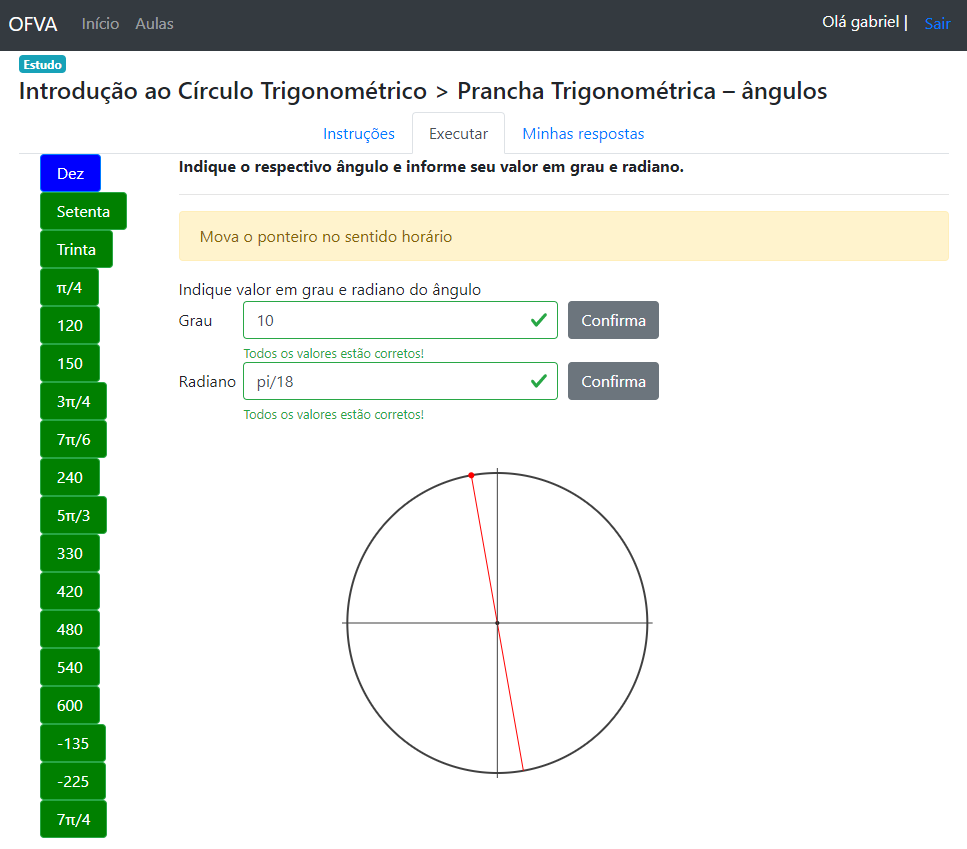
\includegraphics[width=0.9\linewidth]{chapters/results/Fase 3/E2_Virtual.png}
	\caption{Exercício 2 - Ângulos}
	\label{fig:E2}
\end{figure}

É importante salientar que esta atividade contém dezoito casos de teste (ver Apêndice~\ref{Chap:AppendixC}), de modo que em todos os casos é solicitado que o estudante manipule o ponteiro físico até encontrar o ângulo requisitado. Após o envio da resposta física, a interface virtual solicita que sejam inseridos o valor do ângulo em grau e em radiano.

\textbf{Nota Tradicional - $NT$}

Assim como na Seção~\ref{subsubsec:F3A1}, apresentaremos as possibilidades de cálculo da nota tradicional que pode ser baseada nas `entradas' ou `casos de teste', onde nessa segunda opção, há as variantes de cálculo `binário' e `proporcional'. É importante salientar que, embora o Apêndice~\ref{Chap:AppendixAnaliticosA02} contenha a associação entre entradas e pesos dos casos de teste na nota ponderada, esta associação também é utilizada para a nota tradicional, uma vez que o peso 4 corresponde a resposta correta (que é a utilizada na nota tradicional).

A Tabela~\ref{tab:F3_A2_NT_ENTRADAS} apresenta os resultados de $NT$ que foram calculados considerando as três `entradas' do exercício, respectivamente, $EF1$, $EV1$ e $EV2$.


\begin{table}[htbp]
	\centering
	\caption{$NT$ - Cálculo por Entradas}
	\begin{tabular}{|ccccc|}
		\hline
		\rowcolor[HTML]{D0CECE} 
		\multicolumn{5}{|c|}{\cellcolor[HTML]{D0CECE}\textbf{NOTA TRADICIONAL  - ENTRADAS}} \\ \hline
		\rowcolor[HTML]{D0CECE} 
		\multicolumn{1}{|c|}{\cellcolor[HTML]{D0CECE}\textbf{Participante}} &
		\multicolumn{1}{c|}{\cellcolor[HTML]{D0CECE}\textbf{EF1}} &
		\multicolumn{1}{c|}{\cellcolor[HTML]{D0CECE}\textbf{EV1}} &
		\multicolumn{1}{c|}{\cellcolor[HTML]{D0CECE}\textbf{EV2}} &
		\textbf{Média} \\ \hline
		\multicolumn{1}{|c|}{\textbf{B02}} &
		\multicolumn{1}{c|}{9.44} &
		\multicolumn{1}{c|}{10.00} &
		\multicolumn{1}{c|}{10.00} &
		9.815 \\ \hline
		\rowcolor[HTML]{F2F2F2} 
		\multicolumn{1}{|c|}{\cellcolor[HTML]{F2F2F2}\textbf{B03}} &
		\multicolumn{1}{c|}{\cellcolor[HTML]{F2F2F2}10.00} &
		\multicolumn{1}{c|}{\cellcolor[HTML]{F2F2F2}10.00} &
		\multicolumn{1}{c|}{\cellcolor[HTML]{F2F2F2}10.00} &
		10.000 \\ \hline
		\multicolumn{1}{|c|}{\textbf{B04}} &
		\multicolumn{1}{c|}{7.78} &
		\multicolumn{1}{c|}{10.00} &
		\multicolumn{1}{c|}{10.00} &
		9.259 \\ \hline
		\rowcolor[HTML]{F2F2F2} 
		\multicolumn{1}{|c|}{\cellcolor[HTML]{F2F2F2}\textbf{B05}} &
		\multicolumn{1}{c|}{\cellcolor[HTML]{F2F2F2}7.78} &
		\multicolumn{1}{c|}{\cellcolor[HTML]{F2F2F2}10.00} &
		\multicolumn{1}{c|}{\cellcolor[HTML]{F2F2F2}10.00} &
		9.259 \\ \hline
		\multicolumn{1}{|c|}{\textbf{B06}} &
		\multicolumn{1}{c|}{8.89} &
		\multicolumn{1}{c|}{10.00} &
		\multicolumn{1}{c|}{10.00} &
		9.630 \\ \hline
		\rowcolor[HTML]{F2F2F2} 
		\multicolumn{1}{|c|}{\cellcolor[HTML]{F2F2F2}\textbf{B08}} &
		\multicolumn{1}{c|}{\cellcolor[HTML]{F2F2F2}8.89} &
		\multicolumn{1}{c|}{\cellcolor[HTML]{F2F2F2}10.00} &
		\multicolumn{1}{c|}{\cellcolor[HTML]{F2F2F2}10.00} &
		9.630 \\ \hline
		\multicolumn{1}{|c|}{\textbf{B09}} &
		\multicolumn{1}{c|}{9.44} &
		\multicolumn{1}{c|}{10.00} &
		\multicolumn{1}{c|}{10.00} &
		9.815 \\ \hline
		\rowcolor[HTML]{F2F2F2} 
		\multicolumn{1}{|c|}{\cellcolor[HTML]{F2F2F2}\textbf{B10}} &
		\multicolumn{1}{c|}{\cellcolor[HTML]{F2F2F2}9.44} &
		\multicolumn{1}{c|}{\cellcolor[HTML]{F2F2F2}10.00} &
		\multicolumn{1}{c|}{\cellcolor[HTML]{F2F2F2}10.00} &
		9.815 \\ \hline
		\rowcolor[HTML]{D0CECE} 
		\multicolumn{1}{|c|}{\cellcolor[HTML]{D0CECE}\textbf{Média}} &
		\multicolumn{1}{c|}{\cellcolor[HTML]{D0CECE}8.96} &
		\multicolumn{1}{c|}{\cellcolor[HTML]{D0CECE}10.00} &
		\multicolumn{1}{c|}{\cellcolor[HTML]{D0CECE}10.00} &
		9.653 \\ \hline
	\end{tabular}
	\label{tab:F3_A2_NT_ENTRADAS}
\end{table}

Assim, é possível notar que, para todos os participantes, a entrada $EF1$ obteve os menores valores de $NT$ e, portanto, a menor média do grupo. Além disso, os participantes $B04$ e $B05$ obtiveram a menor $NT$ considerando a atividade como um todo.

É importante recordar que o cálculo da nota tradicional utiliza a última resposta dada, e como a atividade pressupõe que o participante tenha `construído' o círculo trigonométrico, é esperado que a $NT$ tenha o valor $10$, de modo que se esse não é o valor obtido, então, é porque a atividade não foi concluída.

Assim, $B03$ foi o único participante do grupo que concluiu a parte do quadro trigonométrico correspondente a Atividade 2, seguindo todas as ajudas fornecidas pelo mesmo, de modo que o resultado final seja o quadro trigonométrico construído com os quadrantes e os dezoito ângulos solicitados.

\begin{table}[htbp]
	\centering
	\caption{$NT$ - Cálculo por Casos de Teste (binário)}
	\begin{tabular}{c|ccccccccc|}
		\cline{2-10}
		\rowcolor[HTML]{D0CECE} 
		\cellcolor[HTML]{F2F2F2}\textbf{} & \multicolumn{9}{c|}{\cellcolor[HTML]{D0CECE}\textbf{Casos de Teste}} \\ \hline
		\rowcolor[HTML]{D9D9D9} 
		\multicolumn{1}{|c|}{\cellcolor[HTML]{D0CECE}\textbf{Participante}} & \multicolumn{1}{c|}{\cellcolor[HTML]{D9D9D9}\textbf{C1}} & \multicolumn{1}{c|}{\cellcolor[HTML]{D9D9D9}\textbf{C2}} & \multicolumn{1}{c|}{\cellcolor[HTML]{D9D9D9}\textbf{C3}} & \multicolumn{1}{c|}{\cellcolor[HTML]{D9D9D9}\textbf{C4}} & \multicolumn{1}{c|}{\cellcolor[HTML]{D9D9D9}\textbf{C5}} & \multicolumn{1}{c|}{\cellcolor[HTML]{D9D9D9}\textbf{C6}} & \multicolumn{1}{c|}{\cellcolor[HTML]{D9D9D9}\textbf{C7}} & \multicolumn{1}{c|}{\cellcolor[HTML]{D9D9D9}\textbf{C8}} & \textbf{C9} \\ \hline
		\multicolumn{1}{|c|}{\textbf{B02}} & \multicolumn{1}{c|}{10.00} & \multicolumn{1}{c|}{10.00} & \multicolumn{1}{c|}{10.00} & \multicolumn{1}{c|}{10.00} & \multicolumn{1}{c|}{0.00} & \multicolumn{1}{c|}{10.00} & \multicolumn{1}{c|}{10.00} & \multicolumn{1}{c|}{10.00} & 10.00 \\ \hline
		\rowcolor[HTML]{F2F2F2} 
		\multicolumn{1}{|c|}{\cellcolor[HTML]{F2F2F2}\textbf{B03}} & \multicolumn{1}{c|}{\cellcolor[HTML]{F2F2F2}10.00} & \multicolumn{1}{c|}{\cellcolor[HTML]{F2F2F2}10.00} & \multicolumn{1}{c|}{\cellcolor[HTML]{F2F2F2}10.00} & \multicolumn{1}{c|}{\cellcolor[HTML]{F2F2F2}10.00} & \multicolumn{1}{c|}{\cellcolor[HTML]{F2F2F2}10.00} & \multicolumn{1}{c|}{\cellcolor[HTML]{F2F2F2}10.00} & \multicolumn{1}{c|}{\cellcolor[HTML]{F2F2F2}10.00} & \multicolumn{1}{c|}{\cellcolor[HTML]{F2F2F2}10.00} & 10.00 \\ \hline
		\multicolumn{1}{|c|}{\textbf{B04}} & \multicolumn{1}{c|}{10.00} & \multicolumn{1}{c|}{10.00} & \multicolumn{1}{c|}{10.00} & \multicolumn{1}{c|}{10.00} & \multicolumn{1}{c|}{10.00} & \multicolumn{1}{c|}{10.00} & \multicolumn{1}{c|}{10.00} & \multicolumn{1}{c|}{0.00} & 0.00 \\ \hline
		\rowcolor[HTML]{F2F2F2} 
		\multicolumn{1}{|c|}{\cellcolor[HTML]{F2F2F2}\textbf{B05}} & \multicolumn{1}{c|}{\cellcolor[HTML]{F2F2F2}10.00} & \multicolumn{1}{c|}{\cellcolor[HTML]{F2F2F2}10.00} & \multicolumn{1}{c|}{\cellcolor[HTML]{F2F2F2}10.00} & \multicolumn{1}{c|}{\cellcolor[HTML]{F2F2F2}10.00} & \multicolumn{1}{c|}{\cellcolor[HTML]{F2F2F2}10.00} & \multicolumn{1}{c|}{\cellcolor[HTML]{F2F2F2}0.00} & \multicolumn{1}{c|}{\cellcolor[HTML]{F2F2F2}10.00} & \multicolumn{1}{c|}{\cellcolor[HTML]{F2F2F2}10.00} & 10.00 \\ \hline
		\multicolumn{1}{|c|}{\textbf{B06}} & \multicolumn{1}{c|}{10.00} & \multicolumn{1}{c|}{10.00} & \multicolumn{1}{c|}{10.00} & \multicolumn{1}{c|}{10.00} & \multicolumn{1}{c|}{0.00} & \multicolumn{1}{c|}{10.00} & \multicolumn{1}{c|}{10.00} & \multicolumn{1}{c|}{10.00} & 10.00 \\ \hline
		\rowcolor[HTML]{F2F2F2} 
		\multicolumn{1}{|c|}{\cellcolor[HTML]{F2F2F2}\textbf{B08}} & \multicolumn{1}{c|}{\cellcolor[HTML]{F2F2F2}10.00} & \multicolumn{1}{c|}{\cellcolor[HTML]{F2F2F2}10.00} & \multicolumn{1}{c|}{\cellcolor[HTML]{F2F2F2}0.00} & \multicolumn{1}{c|}{\cellcolor[HTML]{F2F2F2}10.00} & \multicolumn{1}{c|}{\cellcolor[HTML]{F2F2F2}10.00} & \multicolumn{1}{c|}{\cellcolor[HTML]{F2F2F2}10.00} & \multicolumn{1}{c|}{\cellcolor[HTML]{F2F2F2}10.00} & \multicolumn{1}{c|}{\cellcolor[HTML]{F2F2F2}10.00} & 10.00 \\ \hline
		\multicolumn{1}{|c|}{\textbf{B09}} & \multicolumn{1}{c|}{10.00} & \multicolumn{1}{c|}{10.00} & \multicolumn{1}{c|}{10.00} & \multicolumn{1}{c|}{10.00} & \multicolumn{1}{c|}{10.00} & \multicolumn{1}{c|}{10.00} & \multicolumn{1}{c|}{10.00} & \multicolumn{1}{c|}{10.00} & 10.00 \\ \hline
		\rowcolor[HTML]{F2F2F2} 
		\multicolumn{1}{|c|}{\cellcolor[HTML]{F2F2F2}\textbf{B10}} & \multicolumn{1}{c|}{\cellcolor[HTML]{F2F2F2}10.00} & \multicolumn{1}{c|}{\cellcolor[HTML]{F2F2F2}10.00} & \multicolumn{1}{c|}{\cellcolor[HTML]{F2F2F2}10.00} & \multicolumn{1}{c|}{\cellcolor[HTML]{F2F2F2}10.00} & \multicolumn{1}{c|}{\cellcolor[HTML]{F2F2F2}10.00} & \multicolumn{1}{c|}{\cellcolor[HTML]{F2F2F2}10.00} & \multicolumn{1}{c|}{\cellcolor[HTML]{F2F2F2}10.00} & \multicolumn{1}{c|}{\cellcolor[HTML]{F2F2F2}10.00} & 10.00 \\ \hline
		\rowcolor[HTML]{D0CECE} 
		\multicolumn{1}{|c|}{\cellcolor[HTML]{D0CECE}\textbf{Média}} & \multicolumn{1}{c|}{\cellcolor[HTML]{D0CECE}10.00} & \multicolumn{1}{c|}{\cellcolor[HTML]{D0CECE}10.00} & \multicolumn{1}{c|}{\cellcolor[HTML]{D0CECE}8.75} & \multicolumn{1}{c|}{\cellcolor[HTML]{D0CECE}10.00} & \multicolumn{1}{c|}{\cellcolor[HTML]{D0CECE}7.50} & \multicolumn{1}{c|}{\cellcolor[HTML]{D0CECE}8.75} & \multicolumn{1}{c|}{\cellcolor[HTML]{D0CECE}10.00} & \multicolumn{1}{c|}{\cellcolor[HTML]{D0CECE}8.75} & 8.75 \\ \hline
	\end{tabular}
	\label{tab:F3_A2_NT_CASO_BINARIO}
\end{table}

As Tabelas~\ref{tab:F3_A2_NT_CASO_BINARIO} e~\ref{tab:F3_A2_NT_CASO_BINARIO_} exibem os resultados da nota tradicional, de modo que todas as entradas estão consolidadas em cada um dos casos de teste apresentados. Assim, observa-se que os casos $C1$, $C2$, $C4$, $C7$, $C13$, $C14$ e $C18$ foram concluídos por todos os participantes, enquanto os casos $C5$, $C12$, $C15$ e $C17$ são os casos com menor índice de conclusão.

\begin{table}[htbp]
	\centering
	\caption{$NT$ - Cálculo por Casos de Teste (binário)}
	\begin{tabular}{c|cccccccccc|}
		\cline{2-11}
		\rowcolor[HTML]{D0CECE} 
		\cellcolor[HTML]{F2F2F2}\textbf{} & \multicolumn{10}{c|}{\cellcolor[HTML]{D0CECE}\textbf{Casos de Teste}} \\ \hline
		\rowcolor[HTML]{D9D9D9} 
		\multicolumn{1}{|c|}{\cellcolor[HTML]{D0CECE}\textbf{Part.}} & \multicolumn{1}{c|}{\cellcolor[HTML]{D9D9D9}\textbf{C10}} & \multicolumn{1}{c|}{\cellcolor[HTML]{D9D9D9}\textbf{C11}} & \multicolumn{1}{c|}{\cellcolor[HTML]{D9D9D9}\textbf{C12}} & \multicolumn{1}{c|}{\cellcolor[HTML]{D9D9D9}\textbf{C13}} & \multicolumn{1}{c|}{\cellcolor[HTML]{D9D9D9}\textbf{C14}} & \multicolumn{1}{c|}{\cellcolor[HTML]{D9D9D9}\textbf{C15}} & \multicolumn{1}{c|}{\cellcolor[HTML]{D9D9D9}\textbf{C16}} & \multicolumn{1}{c|}{\cellcolor[HTML]{D9D9D9}\textbf{C17}} & \multicolumn{1}{c|}{\cellcolor[HTML]{D9D9D9}\textbf{C18}} & \textbf{Média} \\ \hline
		\multicolumn{1}{|c|}{\textbf{B02}} & \multicolumn{1}{c|}{10.00} & \multicolumn{1}{c|}{10.00} & \multicolumn{1}{c|}{10.00} & \multicolumn{1}{c|}{10.00} & \multicolumn{1}{c|}{10.00} & \multicolumn{1}{c|}{10.00} & \multicolumn{1}{c|}{10.00} & \multicolumn{1}{c|}{10.00} & \multicolumn{1}{c|}{10.00} & 9.444 \\ \hline
		\rowcolor[HTML]{F2F2F2} 
		\multicolumn{1}{|c|}{\cellcolor[HTML]{F2F2F2}\textbf{B03}} & \multicolumn{1}{c|}{\cellcolor[HTML]{F2F2F2}10.00} & \multicolumn{1}{c|}{\cellcolor[HTML]{F2F2F2}10.00} & \multicolumn{1}{c|}{\cellcolor[HTML]{F2F2F2}10.00} & \multicolumn{1}{c|}{\cellcolor[HTML]{F2F2F2}10.00} & \multicolumn{1}{c|}{\cellcolor[HTML]{F2F2F2}10.00} & \multicolumn{1}{c|}{\cellcolor[HTML]{F2F2F2}10.00} & \multicolumn{1}{c|}{\cellcolor[HTML]{F2F2F2}10.00} & \multicolumn{1}{c|}{\cellcolor[HTML]{F2F2F2}10.00} & \multicolumn{1}{c|}{\cellcolor[HTML]{F2F2F2}10.00} & 10.000 \\ \hline
		\multicolumn{1}{|c|}{\textbf{B04}} & \multicolumn{1}{c|}{10.00} & \multicolumn{1}{c|}{10.00} & \multicolumn{1}{c|}{0.00} & \multicolumn{1}{c|}{10.00} & \multicolumn{1}{c|}{10.00} & \multicolumn{1}{c|}{0.00} & \multicolumn{1}{c|}{10.00} & \multicolumn{1}{c|}{10.00} & \multicolumn{1}{c|}{10.00} & 7.778 \\ \hline
		\rowcolor[HTML]{F2F2F2} 
		\multicolumn{1}{|c|}{\cellcolor[HTML]{F2F2F2}\textbf{B05}} & \multicolumn{1}{c|}{\cellcolor[HTML]{F2F2F2}0.00} & \multicolumn{1}{c|}{\cellcolor[HTML]{F2F2F2}10.00} & \multicolumn{1}{c|}{\cellcolor[HTML]{F2F2F2}10.00} & \multicolumn{1}{c|}{\cellcolor[HTML]{F2F2F2}10.00} & \multicolumn{1}{c|}{\cellcolor[HTML]{F2F2F2}10.00} & \multicolumn{1}{c|}{\cellcolor[HTML]{F2F2F2}0.00} & \multicolumn{1}{c|}{\cellcolor[HTML]{F2F2F2}0.00} & \multicolumn{1}{c|}{\cellcolor[HTML]{F2F2F2}10.00} & \multicolumn{1}{c|}{\cellcolor[HTML]{F2F2F2}10.00} & 7.778 \\ \hline
		\multicolumn{1}{|c|}{\textbf{B06}} & \multicolumn{1}{c|}{10.00} & \multicolumn{1}{c|}{0.00} & \multicolumn{1}{c|}{10.00} & \multicolumn{1}{c|}{10.00} & \multicolumn{1}{c|}{10.00} & \multicolumn{1}{c|}{10.00} & \multicolumn{1}{c|}{10.00} & \multicolumn{1}{c|}{10.00} & \multicolumn{1}{c|}{10.00} & 8.889 \\ \hline
		\rowcolor[HTML]{F2F2F2} 
		\multicolumn{1}{|c|}{\cellcolor[HTML]{F2F2F2}\textbf{B08}} & \multicolumn{1}{c|}{\cellcolor[HTML]{F2F2F2}10.00} & \multicolumn{1}{c|}{\cellcolor[HTML]{F2F2F2}10.00} & \multicolumn{1}{c|}{\cellcolor[HTML]{F2F2F2}10.00} & \multicolumn{1}{c|}{\cellcolor[HTML]{F2F2F2}10.00} & \multicolumn{1}{c|}{\cellcolor[HTML]{F2F2F2}10.00} & \multicolumn{1}{c|}{\cellcolor[HTML]{F2F2F2}10.00} & \multicolumn{1}{c|}{\cellcolor[HTML]{F2F2F2}10.00} & \multicolumn{1}{c|}{\cellcolor[HTML]{F2F2F2}0.00} & \multicolumn{1}{c|}{\cellcolor[HTML]{F2F2F2}10.00} & 8.889 \\ \hline
		\multicolumn{1}{|c|}{\textbf{B09}} & \multicolumn{1}{c|}{10.00} & \multicolumn{1}{c|}{10.00} & \multicolumn{1}{c|}{0.00} & \multicolumn{1}{c|}{10.00} & \multicolumn{1}{c|}{10.00} & \multicolumn{1}{c|}{10.00} & \multicolumn{1}{c|}{10.00} & \multicolumn{1}{c|}{10.00} & \multicolumn{1}{c|}{10.00} & 9.444 \\ \hline
		\rowcolor[HTML]{F2F2F2} 
		\multicolumn{1}{|c|}{\cellcolor[HTML]{F2F2F2}\textbf{B10}} & \multicolumn{1}{c|}{\cellcolor[HTML]{F2F2F2}10.00} & \multicolumn{1}{c|}{\cellcolor[HTML]{F2F2F2}10.00} & \multicolumn{1}{c|}{\cellcolor[HTML]{F2F2F2}10.00} & \multicolumn{1}{c|}{\cellcolor[HTML]{F2F2F2}10.00} & \multicolumn{1}{c|}{\cellcolor[HTML]{F2F2F2}10.00} & \multicolumn{1}{c|}{\cellcolor[HTML]{F2F2F2}10.00} & \multicolumn{1}{c|}{\cellcolor[HTML]{F2F2F2}10.00} & \multicolumn{1}{c|}{\cellcolor[HTML]{F2F2F2}0.00} & \multicolumn{1}{c|}{\cellcolor[HTML]{F2F2F2}10.00} & 9.444 \\ \hline
		\rowcolor[HTML]{D0CECE} 
		\multicolumn{1}{|c|}{\cellcolor[HTML]{D0CECE}\textbf{Média}} & \multicolumn{1}{c|}{\cellcolor[HTML]{D0CECE}8.75} & \multicolumn{1}{c|}{\cellcolor[HTML]{D0CECE}8.75} & \multicolumn{1}{c|}{\cellcolor[HTML]{D0CECE}7.50} & \multicolumn{1}{c|}{\cellcolor[HTML]{D0CECE}10.00} & \multicolumn{1}{c|}{\cellcolor[HTML]{D0CECE}10.00} & \multicolumn{1}{c|}{\cellcolor[HTML]{D0CECE}7.50} & \multicolumn{1}{c|}{\cellcolor[HTML]{D0CECE}8.75} & \multicolumn{1}{c|}{\cellcolor[HTML]{D0CECE}7.50} & \multicolumn{1}{c|}{\cellcolor[HTML]{D0CECE}10.00} & 8.958 \\ \hline
	\end{tabular}
	\label{tab:F3_A2_NT_CASO_BINARIO_}
\end{table}

Do ponto de vista dos participantes, a coluna `Média' da Tabela~\ref{tab:F3_A2_NT_CASO_BINARIO_} apresenta as notas tradicionais do exercício inteiro para cada indivíduo, de modo que, tal como na Tabela~\ref{tab:F3_A2_NP_ENTRADAS}, os participantes $B4$ e $B5$ foram os que obtiveram menor nota tradicional, sendo $7.778$ para ambos.

%\begin{table}[htbp]
%	\centering
%	\caption{$NT$ - Cálculo por Casos de Teste (binário)}
%	\begin{tabular}{c|ccccccccccccccccccc|}
%		\cline{2-20}
%		\rowcolor[HTML]{D0CECE} 
%		\cellcolor[HTML]{F2F2F2}\textbf{} & \multicolumn{19}{c|}{\cellcolor[HTML]{D0CECE}\textbf{Casos de Teste}} \\ \hline
%		\rowcolor[HTML]{D9D9D9} 
%		\multicolumn{1}{|c|}{\cellcolor[HTML]{D0CECE}\textbf{Part.}} & \multicolumn{1}{c|}{\cellcolor[HTML]{D9D9D9}\textbf{C1}} & \multicolumn{1}{c|}{\cellcolor[HTML]{D9D9D9}\textbf{C2}} & \multicolumn{1}{c|}{\cellcolor[HTML]{D9D9D9}\textbf{C3}} & \multicolumn{1}{c|}{\cellcolor[HTML]{D9D9D9}\textbf{C4}} & \multicolumn{1}{c|}{\cellcolor[HTML]{D9D9D9}\textbf{C5}} & \multicolumn{1}{c|}{\cellcolor[HTML]{D9D9D9}\textbf{C6}} & \multicolumn{1}{c|}{\cellcolor[HTML]{D9D9D9}\textbf{C7}} & \multicolumn{1}{c|}{\cellcolor[HTML]{D9D9D9}\textbf{C8}} & \multicolumn{1}{c|}{\cellcolor[HTML]{D9D9D9}\textbf{C9}} & \multicolumn{1}{c|}{\cellcolor[HTML]{D9D9D9}\textbf{C10}} & \multicolumn{1}{c|}{\cellcolor[HTML]{D9D9D9}\textbf{C11}} & \multicolumn{1}{c|}{\cellcolor[HTML]{D9D9D9}\textbf{C12}} & \multicolumn{1}{c|}{\cellcolor[HTML]{D9D9D9}\textbf{C13}} & \multicolumn{1}{c|}{\cellcolor[HTML]{D9D9D9}\textbf{C14}} & \multicolumn{1}{c|}{\cellcolor[HTML]{D9D9D9}\textbf{C15}} & \multicolumn{1}{c|}{\cellcolor[HTML]{D9D9D9}\textbf{C16}} & \multicolumn{1}{c|}{\cellcolor[HTML]{D9D9D9}\textbf{C17}} & \multicolumn{1}{c|}{\cellcolor[HTML]{D9D9D9}\textbf{C18}} & \textbf{Média} \\ \hline
%		\multicolumn{1}{|c|}{\textbf{B02}} & \multicolumn{1}{c|}{10.00} & \multicolumn{1}{c|}{10.00} & \multicolumn{1}{c|}{10.00} & \multicolumn{1}{c|}{10.00} & \multicolumn{1}{c|}{0.00} & \multicolumn{1}{c|}{10.00} & \multicolumn{1}{c|}{10.00} & \multicolumn{1}{c|}{10.00} & \multicolumn{1}{c|}{10.00} & \multicolumn{1}{c|}{10.00} & \multicolumn{1}{c|}{10.00} & \multicolumn{1}{c|}{10.00} & \multicolumn{1}{c|}{10.00} & \multicolumn{1}{c|}{10.00} & \multicolumn{1}{c|}{10.00} & \multicolumn{1}{c|}{10.00} & \multicolumn{1}{c|}{10.00} & \multicolumn{1}{c|}{10.00} & 9.444 \\ \hline
%		\rowcolor[HTML]{F2F2F2} 
%		\multicolumn{1}{|c|}{\cellcolor[HTML]{F2F2F2}\textbf{B03}} & \multicolumn{1}{c|}{\cellcolor[HTML]{F2F2F2}10.00} & \multicolumn{1}{c|}{\cellcolor[HTML]{F2F2F2}10.00} & \multicolumn{1}{c|}{\cellcolor[HTML]{F2F2F2}10.00} & \multicolumn{1}{c|}{\cellcolor[HTML]{F2F2F2}10.00} & \multicolumn{1}{c|}{\cellcolor[HTML]{F2F2F2}10.00} & \multicolumn{1}{c|}{\cellcolor[HTML]{F2F2F2}10.00} & \multicolumn{1}{c|}{\cellcolor[HTML]{F2F2F2}10.00} & \multicolumn{1}{c|}{\cellcolor[HTML]{F2F2F2}10.00} & \multicolumn{1}{c|}{\cellcolor[HTML]{F2F2F2}10.00} & \multicolumn{1}{c|}{\cellcolor[HTML]{F2F2F2}10.00} & \multicolumn{1}{c|}{\cellcolor[HTML]{F2F2F2}10.00} & \multicolumn{1}{c|}{\cellcolor[HTML]{F2F2F2}10.00} & \multicolumn{1}{c|}{\cellcolor[HTML]{F2F2F2}10.00} & \multicolumn{1}{c|}{\cellcolor[HTML]{F2F2F2}10.00} & \multicolumn{1}{c|}{\cellcolor[HTML]{F2F2F2}10.00} & \multicolumn{1}{c|}{\cellcolor[HTML]{F2F2F2}10.00} & \multicolumn{1}{c|}{\cellcolor[HTML]{F2F2F2}10.00} & \multicolumn{1}{c|}{\cellcolor[HTML]{F2F2F2}10.00} & 10.000 \\ \hline
%		\multicolumn{1}{|c|}{\textbf{B04}} & \multicolumn{1}{c|}{10.00} & \multicolumn{1}{c|}{10.00} & \multicolumn{1}{c|}{10.00} & \multicolumn{1}{c|}{10.00} & \multicolumn{1}{c|}{10.00} & \multicolumn{1}{c|}{10.00} & \multicolumn{1}{c|}{10.00} & \multicolumn{1}{c|}{0.00} & \multicolumn{1}{c|}{0.00} & \multicolumn{1}{c|}{10.00} & \multicolumn{1}{c|}{10.00} & \multicolumn{1}{c|}{0.00} & \multicolumn{1}{c|}{10.00} & \multicolumn{1}{c|}{10.00} & \multicolumn{1}{c|}{0.00} & \multicolumn{1}{c|}{10.00} & \multicolumn{1}{c|}{10.00} & \multicolumn{1}{c|}{10.00} & 7.778 \\ \hline
%		\rowcolor[HTML]{F2F2F2} 
%		\multicolumn{1}{|c|}{\cellcolor[HTML]{F2F2F2}\textbf{B05}} & \multicolumn{1}{c|}{\cellcolor[HTML]{F2F2F2}10.00} & \multicolumn{1}{c|}{\cellcolor[HTML]{F2F2F2}10.00} & \multicolumn{1}{c|}{\cellcolor[HTML]{F2F2F2}10.00} & \multicolumn{1}{c|}{\cellcolor[HTML]{F2F2F2}10.00} & \multicolumn{1}{c|}{\cellcolor[HTML]{F2F2F2}10.00} & \multicolumn{1}{c|}{\cellcolor[HTML]{F2F2F2}0.00} & \multicolumn{1}{c|}{\cellcolor[HTML]{F2F2F2}10.00} & \multicolumn{1}{c|}{\cellcolor[HTML]{F2F2F2}10.00} & \multicolumn{1}{c|}{\cellcolor[HTML]{F2F2F2}10.00} & \multicolumn{1}{c|}{\cellcolor[HTML]{F2F2F2}0.00} & \multicolumn{1}{c|}{\cellcolor[HTML]{F2F2F2}10.00} & \multicolumn{1}{c|}{\cellcolor[HTML]{F2F2F2}10.00} & \multicolumn{1}{c|}{\cellcolor[HTML]{F2F2F2}10.00} & \multicolumn{1}{c|}{\cellcolor[HTML]{F2F2F2}10.00} & \multicolumn{1}{c|}{\cellcolor[HTML]{F2F2F2}0.00} & \multicolumn{1}{c|}{\cellcolor[HTML]{F2F2F2}0.00} & \multicolumn{1}{c|}{\cellcolor[HTML]{F2F2F2}10.00} & \multicolumn{1}{c|}{\cellcolor[HTML]{F2F2F2}10.00} & 7.778 \\ \hline
%		\multicolumn{1}{|c|}{\textbf{B06}} & \multicolumn{1}{c|}{10.00} & \multicolumn{1}{c|}{10.00} & \multicolumn{1}{c|}{10.00} & \multicolumn{1}{c|}{10.00} & \multicolumn{1}{c|}{0.00} & \multicolumn{1}{c|}{10.00} & \multicolumn{1}{c|}{10.00} & \multicolumn{1}{c|}{10.00} & \multicolumn{1}{c|}{10.00} & \multicolumn{1}{c|}{10.00} & \multicolumn{1}{c|}{0.00} & \multicolumn{1}{c|}{10.00} & \multicolumn{1}{c|}{10.00} & \multicolumn{1}{c|}{10.00} & \multicolumn{1}{c|}{10.00} & \multicolumn{1}{c|}{10.00} & \multicolumn{1}{c|}{10.00} & \multicolumn{1}{c|}{10.00} & 8.889 \\ \hline
%		\rowcolor[HTML]{F2F2F2} 
%		\multicolumn{1}{|c|}{\cellcolor[HTML]{F2F2F2}\textbf{B08}} & \multicolumn{1}{c|}{\cellcolor[HTML]{F2F2F2}10.00} & \multicolumn{1}{c|}{\cellcolor[HTML]{F2F2F2}10.00} & \multicolumn{1}{c|}{\cellcolor[HTML]{F2F2F2}0.00} & \multicolumn{1}{c|}{\cellcolor[HTML]{F2F2F2}10.00} & \multicolumn{1}{c|}{\cellcolor[HTML]{F2F2F2}10.00} & \multicolumn{1}{c|}{\cellcolor[HTML]{F2F2F2}10.00} & \multicolumn{1}{c|}{\cellcolor[HTML]{F2F2F2}10.00} & \multicolumn{1}{c|}{\cellcolor[HTML]{F2F2F2}10.00} & \multicolumn{1}{c|}{\cellcolor[HTML]{F2F2F2}10.00} & \multicolumn{1}{c|}{\cellcolor[HTML]{F2F2F2}10.00} & \multicolumn{1}{c|}{\cellcolor[HTML]{F2F2F2}10.00} & \multicolumn{1}{c|}{\cellcolor[HTML]{F2F2F2}10.00} & \multicolumn{1}{c|}{\cellcolor[HTML]{F2F2F2}10.00} & \multicolumn{1}{c|}{\cellcolor[HTML]{F2F2F2}10.00} & \multicolumn{1}{c|}{\cellcolor[HTML]{F2F2F2}10.00} & \multicolumn{1}{c|}{\cellcolor[HTML]{F2F2F2}10.00} & \multicolumn{1}{c|}{\cellcolor[HTML]{F2F2F2}0.00} & \multicolumn{1}{c|}{\cellcolor[HTML]{F2F2F2}10.00} & 8.889 \\ \hline
%		\multicolumn{1}{|c|}{\textbf{B09}} & \multicolumn{1}{c|}{10.00} & \multicolumn{1}{c|}{10.00} & \multicolumn{1}{c|}{10.00} & \multicolumn{1}{c|}{10.00} & \multicolumn{1}{c|}{10.00} & \multicolumn{1}{c|}{10.00} & \multicolumn{1}{c|}{10.00} & \multicolumn{1}{c|}{10.00} & \multicolumn{1}{c|}{10.00} & \multicolumn{1}{c|}{10.00} & \multicolumn{1}{c|}{10.00} & \multicolumn{1}{c|}{0.00} & \multicolumn{1}{c|}{10.00} & \multicolumn{1}{c|}{10.00} & \multicolumn{1}{c|}{10.00} & \multicolumn{1}{c|}{10.00} & \multicolumn{1}{c|}{10.00} & \multicolumn{1}{c|}{10.00} & 9.444 \\ \hline
%		\rowcolor[HTML]{F2F2F2} 
%		\multicolumn{1}{|c|}{\cellcolor[HTML]{F2F2F2}\textbf{B10}} & \multicolumn{1}{c|}{\cellcolor[HTML]{F2F2F2}10.00} & \multicolumn{1}{c|}{\cellcolor[HTML]{F2F2F2}10.00} & \multicolumn{1}{c|}{\cellcolor[HTML]{F2F2F2}10.00} & \multicolumn{1}{c|}{\cellcolor[HTML]{F2F2F2}10.00} & \multicolumn{1}{c|}{\cellcolor[HTML]{F2F2F2}10.00} & \multicolumn{1}{c|}{\cellcolor[HTML]{F2F2F2}10.00} & \multicolumn{1}{c|}{\cellcolor[HTML]{F2F2F2}10.00} & \multicolumn{1}{c|}{\cellcolor[HTML]{F2F2F2}10.00} & \multicolumn{1}{c|}{\cellcolor[HTML]{F2F2F2}10.00} & \multicolumn{1}{c|}{\cellcolor[HTML]{F2F2F2}10.00} & \multicolumn{1}{c|}{\cellcolor[HTML]{F2F2F2}10.00} & \multicolumn{1}{c|}{\cellcolor[HTML]{F2F2F2}10.00} & \multicolumn{1}{c|}{\cellcolor[HTML]{F2F2F2}10.00} & \multicolumn{1}{c|}{\cellcolor[HTML]{F2F2F2}10.00} & \multicolumn{1}{c|}{\cellcolor[HTML]{F2F2F2}10.00} & \multicolumn{1}{c|}{\cellcolor[HTML]{F2F2F2}10.00} & \multicolumn{1}{c|}{\cellcolor[HTML]{F2F2F2}0.00} & \multicolumn{1}{c|}{\cellcolor[HTML]{F2F2F2}10.00} & 9.444 \\ \hline
%		\rowcolor[HTML]{D0CECE} 
%		\multicolumn{1}{|c|}{\cellcolor[HTML]{D0CECE}\textbf{Média}} & \multicolumn{1}{c|}{\cellcolor[HTML]{D0CECE}10.00} & \multicolumn{1}{c|}{\cellcolor[HTML]{D0CECE}10.00} & \multicolumn{1}{c|}{\cellcolor[HTML]{D0CECE}8.75} & \multicolumn{1}{c|}{\cellcolor[HTML]{D0CECE}10.00} & \multicolumn{1}{c|}{\cellcolor[HTML]{D0CECE}7.50} & \multicolumn{1}{c|}{\cellcolor[HTML]{D0CECE}8.75} & \multicolumn{1}{c|}{\cellcolor[HTML]{D0CECE}10.00} & \multicolumn{1}{c|}{\cellcolor[HTML]{D0CECE}8.75} & \multicolumn{1}{c|}{\cellcolor[HTML]{D0CECE}8.75} & \multicolumn{1}{c|}{\cellcolor[HTML]{D0CECE}8.75} & \multicolumn{1}{c|}{\cellcolor[HTML]{D0CECE}8.75} & \multicolumn{1}{c|}{\cellcolor[HTML]{D0CECE}7.50} & \multicolumn{1}{c|}{\cellcolor[HTML]{D0CECE}10.00} & \multicolumn{1}{c|}{\cellcolor[HTML]{D0CECE}10.00} & \multicolumn{1}{c|}{\cellcolor[HTML]{D0CECE}7.50} & \multicolumn{1}{c|}{\cellcolor[HTML]{D0CECE}8.75} & \multicolumn{1}{c|}{\cellcolor[HTML]{D0CECE}7.50} & \multicolumn{1}{c|}{\cellcolor[HTML]{D0CECE}10.00} & 8.958 \\ \hline
%	\end{tabular}
%	\label{tab:F3_A2_NT_CASO_BINARIO}
%\end{table}

\begin{table}[htbp]
	\centering
	\caption{$NT$ - Cálculo por Casos de Teste (proporcional)}
	\begin{tabular}{c|ccccccccc|}
		\cline{2-10}
		\rowcolor[HTML]{D0CECE} 
		\cellcolor[HTML]{F2F2F2}\textbf{} & \multicolumn{9}{c|}{\cellcolor[HTML]{D0CECE}\textbf{Casos de Teste}} \\ \hline
		\rowcolor[HTML]{D9D9D9} 
		\multicolumn{1}{|c|}{\cellcolor[HTML]{D0CECE}\textbf{Participante}} & \multicolumn{1}{c|}{\cellcolor[HTML]{D9D9D9}\textbf{C1}} & \multicolumn{1}{c|}{\cellcolor[HTML]{D9D9D9}\textbf{C2}} & \multicolumn{1}{c|}{\cellcolor[HTML]{D9D9D9}\textbf{C3}} & \multicolumn{1}{c|}{\cellcolor[HTML]{D9D9D9}\textbf{C4}} & \multicolumn{1}{c|}{\cellcolor[HTML]{D9D9D9}\textbf{C5}} & \multicolumn{1}{c|}{\cellcolor[HTML]{D9D9D9}\textbf{C6}} & \multicolumn{1}{c|}{\cellcolor[HTML]{D9D9D9}\textbf{C7}} & \multicolumn{1}{c|}{\cellcolor[HTML]{D9D9D9}\textbf{C8}} & \textbf{C9} \\ \hline
		\multicolumn{1}{|c|}{\textbf{B02}} & \multicolumn{1}{c|}{10.00} & \multicolumn{1}{c|}{10.00} & \multicolumn{1}{c|}{10.00} & \multicolumn{1}{c|}{10.00} & \multicolumn{1}{c|}{6.67} & \multicolumn{1}{c|}{10.00} & \multicolumn{1}{c|}{10.00} & \multicolumn{1}{c|}{10.00} & 10.00 \\ \hline
		\rowcolor[HTML]{F2F2F2} 
		\multicolumn{1}{|c|}{\cellcolor[HTML]{F2F2F2}\textbf{B03}} & \multicolumn{1}{c|}{\cellcolor[HTML]{F2F2F2}10.00} & \multicolumn{1}{c|}{\cellcolor[HTML]{F2F2F2}10.00} & \multicolumn{1}{c|}{\cellcolor[HTML]{F2F2F2}10.00} & \multicolumn{1}{c|}{\cellcolor[HTML]{F2F2F2}10.00} & \multicolumn{1}{c|}{\cellcolor[HTML]{F2F2F2}10.00} & \multicolumn{1}{c|}{\cellcolor[HTML]{F2F2F2}10.00} & \multicolumn{1}{c|}{\cellcolor[HTML]{F2F2F2}10.00} & \multicolumn{1}{c|}{\cellcolor[HTML]{F2F2F2}10.00} & 10.00 \\ \hline
		\multicolumn{1}{|c|}{\textbf{B04}} & \multicolumn{1}{c|}{10.00} & \multicolumn{1}{c|}{10.00} & \multicolumn{1}{c|}{10.00} & \multicolumn{1}{c|}{10.00} & \multicolumn{1}{c|}{10.00} & \multicolumn{1}{c|}{10.00} & \multicolumn{1}{c|}{10.00} & \multicolumn{1}{c|}{6.67} & 6.67 \\ \hline
		\rowcolor[HTML]{F2F2F2} 
		\multicolumn{1}{|c|}{\cellcolor[HTML]{F2F2F2}\textbf{B05}} & \multicolumn{1}{c|}{\cellcolor[HTML]{F2F2F2}10.00} & \multicolumn{1}{c|}{\cellcolor[HTML]{F2F2F2}10.00} & \multicolumn{1}{c|}{\cellcolor[HTML]{F2F2F2}10.00} & \multicolumn{1}{c|}{\cellcolor[HTML]{F2F2F2}10.00} & \multicolumn{1}{c|}{\cellcolor[HTML]{F2F2F2}10.00} & \multicolumn{1}{c|}{\cellcolor[HTML]{F2F2F2}6.67} & \multicolumn{1}{c|}{\cellcolor[HTML]{F2F2F2}10.00} & \multicolumn{1}{c|}{\cellcolor[HTML]{F2F2F2}10.00} & 10.00 \\ \hline
		\multicolumn{1}{|c|}{\textbf{B06}} & \multicolumn{1}{c|}{10.00} & \multicolumn{1}{c|}{10.00} & \multicolumn{1}{c|}{10.00} & \multicolumn{1}{c|}{10.00} & \multicolumn{1}{c|}{6.67} & \multicolumn{1}{c|}{10.00} & \multicolumn{1}{c|}{10.00} & \multicolumn{1}{c|}{10.00} & 10.00 \\ \hline
		\rowcolor[HTML]{F2F2F2} 
		\multicolumn{1}{|c|}{\cellcolor[HTML]{F2F2F2}\textbf{B08}} & \multicolumn{1}{c|}{\cellcolor[HTML]{F2F2F2}10.00} & \multicolumn{1}{c|}{\cellcolor[HTML]{F2F2F2}10.00} & \multicolumn{1}{c|}{\cellcolor[HTML]{F2F2F2}6.67} & \multicolumn{1}{c|}{\cellcolor[HTML]{F2F2F2}10.00} & \multicolumn{1}{c|}{\cellcolor[HTML]{F2F2F2}10.00} & \multicolumn{1}{c|}{\cellcolor[HTML]{F2F2F2}10.00} & \multicolumn{1}{c|}{\cellcolor[HTML]{F2F2F2}10.00} & \multicolumn{1}{c|}{\cellcolor[HTML]{F2F2F2}10.00} & 10.00 \\ \hline
		\multicolumn{1}{|c|}{\textbf{B09}} & \multicolumn{1}{c|}{10.00} & \multicolumn{1}{c|}{10.00} & \multicolumn{1}{c|}{10.00} & \multicolumn{1}{c|}{10.00} & \multicolumn{1}{c|}{10.00} & \multicolumn{1}{c|}{10.00} & \multicolumn{1}{c|}{10.00} & \multicolumn{1}{c|}{10.00} & 10.00 \\ \hline
		\rowcolor[HTML]{F2F2F2} 
		\multicolumn{1}{|c|}{\cellcolor[HTML]{F2F2F2}\textbf{B10}} & \multicolumn{1}{c|}{\cellcolor[HTML]{F2F2F2}10.00} & \multicolumn{1}{c|}{\cellcolor[HTML]{F2F2F2}10.00} & \multicolumn{1}{c|}{\cellcolor[HTML]{F2F2F2}10.00} & \multicolumn{1}{c|}{\cellcolor[HTML]{F2F2F2}10.00} & \multicolumn{1}{c|}{\cellcolor[HTML]{F2F2F2}10.00} & \multicolumn{1}{c|}{\cellcolor[HTML]{F2F2F2}10.00} & \multicolumn{1}{c|}{\cellcolor[HTML]{F2F2F2}10.00} & \multicolumn{1}{c|}{\cellcolor[HTML]{F2F2F2}10.00} & 10.00 \\ \hline
		\rowcolor[HTML]{D0CECE} 
		\multicolumn{1}{|c|}{\cellcolor[HTML]{D0CECE}\textbf{Média}} & \multicolumn{1}{c|}{\cellcolor[HTML]{D0CECE}10.00} & \multicolumn{1}{c|}{\cellcolor[HTML]{D0CECE}10.00} & \multicolumn{1}{c|}{\cellcolor[HTML]{D0CECE}9.58} & \multicolumn{1}{c|}{\cellcolor[HTML]{D0CECE}10.00} & \multicolumn{1}{c|}{\cellcolor[HTML]{D0CECE}9.17} & \multicolumn{1}{c|}{\cellcolor[HTML]{D0CECE}9.58} & \multicolumn{1}{c|}{\cellcolor[HTML]{D0CECE}10.00} & \multicolumn{1}{c|}{\cellcolor[HTML]{D0CECE}9.58} & 9.58 \\ \hline
	\end{tabular}
	\label{tab:F3_A2_NT_CASO_PROPORCIONAL}
\end{table}

As Tabelas~\ref{tab:F3_A2_NT_CASO_PROPORCIONAL} e~\ref{tab:F3_A2_NT_CASO_PROPORCIONAL_} apresentam os resultados de nota tradicional considerando o cálculo proporcional. Ao comparar com a variante `binária', não há diferenças com relação aos casos de teste concluídos ou aos participantes com a menor nota.

\begin{table}[htbp]
	\centering
	\caption{$NT$ - Cálculo por Casos de Teste (proporcional)}
	\begin{tabular}{c|cccccccccc|}
		\cline{2-11}
		\rowcolor[HTML]{D0CECE} 
		\cellcolor[HTML]{F2F2F2}\textbf{} & \multicolumn{10}{c|}{\cellcolor[HTML]{D0CECE}\textbf{Casos de Teste}} \\ \hline
		\rowcolor[HTML]{D9D9D9} 
		\multicolumn{1}{|c|}{\cellcolor[HTML]{D0CECE}\textbf{Part.}} & \multicolumn{1}{c|}{\cellcolor[HTML]{D9D9D9}\textbf{C10}} & \multicolumn{1}{c|}{\cellcolor[HTML]{D9D9D9}\textbf{C11}} & \multicolumn{1}{c|}{\cellcolor[HTML]{D9D9D9}\textbf{C12}} & \multicolumn{1}{c|}{\cellcolor[HTML]{D9D9D9}\textbf{C13}} & \multicolumn{1}{c|}{\cellcolor[HTML]{D9D9D9}\textbf{C14}} & \multicolumn{1}{c|}{\cellcolor[HTML]{D9D9D9}\textbf{C15}} & \multicolumn{1}{c|}{\cellcolor[HTML]{D9D9D9}\textbf{C16}} & \multicolumn{1}{c|}{\cellcolor[HTML]{D9D9D9}\textbf{C17}} & \multicolumn{1}{c|}{\cellcolor[HTML]{D9D9D9}\textbf{C18}} & \textbf{Média} \\ \hline
		\multicolumn{1}{|c|}{\textbf{B02}} & \multicolumn{1}{c|}{10.00} & \multicolumn{1}{c|}{10.00} & \multicolumn{1}{c|}{10.00} & \multicolumn{1}{c|}{10.00} & \multicolumn{1}{c|}{10.00} & \multicolumn{1}{c|}{10.00} & \multicolumn{1}{c|}{10.00} & \multicolumn{1}{c|}{10.00} & \multicolumn{1}{c|}{10.00} & 9.815 \\ \hline
		\rowcolor[HTML]{F2F2F2} 
		\multicolumn{1}{|c|}{\cellcolor[HTML]{F2F2F2}\textbf{B03}} & \multicolumn{1}{c|}{\cellcolor[HTML]{F2F2F2}10.00} & \multicolumn{1}{c|}{\cellcolor[HTML]{F2F2F2}10.00} & \multicolumn{1}{c|}{\cellcolor[HTML]{F2F2F2}10.00} & \multicolumn{1}{c|}{\cellcolor[HTML]{F2F2F2}10.00} & \multicolumn{1}{c|}{\cellcolor[HTML]{F2F2F2}10.00} & \multicolumn{1}{c|}{\cellcolor[HTML]{F2F2F2}10.00} & \multicolumn{1}{c|}{\cellcolor[HTML]{F2F2F2}10.00} & \multicolumn{1}{c|}{\cellcolor[HTML]{F2F2F2}10.00} & \multicolumn{1}{c|}{\cellcolor[HTML]{F2F2F2}10.00} & 10.000 \\ \hline
		\multicolumn{1}{|c|}{\textbf{B04}} & \multicolumn{1}{c|}{10.00} & \multicolumn{1}{c|}{10.00} & \multicolumn{1}{c|}{6.67} & \multicolumn{1}{c|}{10.00} & \multicolumn{1}{c|}{10.00} & \multicolumn{1}{c|}{6.67} & \multicolumn{1}{c|}{10.00} & \multicolumn{1}{c|}{10.00} & \multicolumn{1}{c|}{10.00} & 9.259 \\ \hline
		\rowcolor[HTML]{F2F2F2} 
		\multicolumn{1}{|c|}{\cellcolor[HTML]{F2F2F2}\textbf{B05}} & \multicolumn{1}{c|}{\cellcolor[HTML]{F2F2F2}6.67} & \multicolumn{1}{c|}{\cellcolor[HTML]{F2F2F2}10.00} & \multicolumn{1}{c|}{\cellcolor[HTML]{F2F2F2}10.00} & \multicolumn{1}{c|}{\cellcolor[HTML]{F2F2F2}10.00} & \multicolumn{1}{c|}{\cellcolor[HTML]{F2F2F2}10.00} & \multicolumn{1}{c|}{\cellcolor[HTML]{F2F2F2}6.67} & \multicolumn{1}{c|}{\cellcolor[HTML]{F2F2F2}6.67} & \multicolumn{1}{c|}{\cellcolor[HTML]{F2F2F2}10.00} & \multicolumn{1}{c|}{\cellcolor[HTML]{F2F2F2}10.00} & 9.259 \\ \hline
		\multicolumn{1}{|c|}{\textbf{B06}} & \multicolumn{1}{c|}{10.00} & \multicolumn{1}{c|}{6.67} & \multicolumn{1}{c|}{10.00} & \multicolumn{1}{c|}{10.00} & \multicolumn{1}{c|}{10.00} & \multicolumn{1}{c|}{10.00} & \multicolumn{1}{c|}{10.00} & \multicolumn{1}{c|}{10.00} & \multicolumn{1}{c|}{10.00} & 9.630 \\ \hline
		\rowcolor[HTML]{F2F2F2} 
		\multicolumn{1}{|c|}{\cellcolor[HTML]{F2F2F2}\textbf{B08}} & \multicolumn{1}{c|}{\cellcolor[HTML]{F2F2F2}10.00} & \multicolumn{1}{c|}{\cellcolor[HTML]{F2F2F2}10.00} & \multicolumn{1}{c|}{\cellcolor[HTML]{F2F2F2}10.00} & \multicolumn{1}{c|}{\cellcolor[HTML]{F2F2F2}10.00} & \multicolumn{1}{c|}{\cellcolor[HTML]{F2F2F2}10.00} & \multicolumn{1}{c|}{\cellcolor[HTML]{F2F2F2}10.00} & \multicolumn{1}{c|}{\cellcolor[HTML]{F2F2F2}10.00} & \multicolumn{1}{c|}{\cellcolor[HTML]{F2F2F2}6.67} & \multicolumn{1}{c|}{\cellcolor[HTML]{F2F2F2}10.00} & 9.630 \\ \hline
		\multicolumn{1}{|c|}{\textbf{B09}} & \multicolumn{1}{c|}{10.00} & \multicolumn{1}{c|}{10.00} & \multicolumn{1}{c|}{6.67} & \multicolumn{1}{c|}{10.00} & \multicolumn{1}{c|}{10.00} & \multicolumn{1}{c|}{10.00} & \multicolumn{1}{c|}{10.00} & \multicolumn{1}{c|}{10.00} & \multicolumn{1}{c|}{10.00} & 9.815 \\ \hline
		\rowcolor[HTML]{F2F2F2} 
		\multicolumn{1}{|c|}{\cellcolor[HTML]{F2F2F2}\textbf{B10}} & \multicolumn{1}{c|}{\cellcolor[HTML]{F2F2F2}10.00} & \multicolumn{1}{c|}{\cellcolor[HTML]{F2F2F2}10.00} & \multicolumn{1}{c|}{\cellcolor[HTML]{F2F2F2}10.00} & \multicolumn{1}{c|}{\cellcolor[HTML]{F2F2F2}10.00} & \multicolumn{1}{c|}{\cellcolor[HTML]{F2F2F2}10.00} & \multicolumn{1}{c|}{\cellcolor[HTML]{F2F2F2}10.00} & \multicolumn{1}{c|}{\cellcolor[HTML]{F2F2F2}10.00} & \multicolumn{1}{c|}{\cellcolor[HTML]{F2F2F2}6.67} & \multicolumn{1}{c|}{\cellcolor[HTML]{F2F2F2}10.00} & 9.815 \\ \hline
		\rowcolor[HTML]{D0CECE} 
		\multicolumn{1}{|c|}{\cellcolor[HTML]{D0CECE}\textbf{Média}} & \multicolumn{1}{c|}{\cellcolor[HTML]{D0CECE}9.58} & \multicolumn{1}{c|}{\cellcolor[HTML]{D0CECE}9.58} & \multicolumn{1}{c|}{\cellcolor[HTML]{D0CECE}9.17} & \multicolumn{1}{c|}{\cellcolor[HTML]{D0CECE}10.00} & \multicolumn{1}{c|}{\cellcolor[HTML]{D0CECE}10.00} & \multicolumn{1}{c|}{\cellcolor[HTML]{D0CECE}9.17} & \multicolumn{1}{c|}{\cellcolor[HTML]{D0CECE}9.58} & \multicolumn{1}{c|}{\cellcolor[HTML]{D0CECE}9.17} & \multicolumn{1}{c|}{\cellcolor[HTML]{D0CECE}10.00} & 9.653 \\ \hline
	\end{tabular}
	\label{tab:F3_A2_NT_CASO_PROPORCIONAL_}
\end{table}

Além disso, vale ressaltar que a diferença entre os modos de calcular é observada no valor absoluto da nota tradicional, uma vez que o modo binário considera que todas as entradas de um caso de teste precisam estar corretas para que o caso de teste esteja correto, enquanto o modo proporcional considera a média da exatidão das entradas do caso.

%\begin{table}[htbp]
%	\centering
%	\caption{$NT$ - Cálculo por Casos de Teste (proporcional)}
%	\begin{tabular}{c|ccccccccccccccccccc|}
%		\cline{2-20}
%		\rowcolor[HTML]{D0CECE} 
%		\cellcolor[HTML]{F2F2F2}\textbf{} & \multicolumn{19}{c|}{\cellcolor[HTML]{D0CECE}\textbf{Casos de Teste}} \\ \hline
%		\rowcolor[HTML]{D9D9D9} 
%		\multicolumn{1}{|c|}{\cellcolor[HTML]{D0CECE}\textbf{Part.}} & \multicolumn{1}{c|}{\cellcolor[HTML]{D9D9D9}\textbf{C1}} & \multicolumn{1}{c|}{\cellcolor[HTML]{D9D9D9}\textbf{C2}} & \multicolumn{1}{c|}{\cellcolor[HTML]{D9D9D9}\textbf{C3}} & \multicolumn{1}{c|}{\cellcolor[HTML]{D9D9D9}\textbf{C4}} & \multicolumn{1}{c|}{\cellcolor[HTML]{D9D9D9}\textbf{C5}} & \multicolumn{1}{c|}{\cellcolor[HTML]{D9D9D9}\textbf{C6}} & \multicolumn{1}{c|}{\cellcolor[HTML]{D9D9D9}\textbf{C7}} & \multicolumn{1}{c|}{\cellcolor[HTML]{D9D9D9}\textbf{C8}} & \multicolumn{1}{c|}{\cellcolor[HTML]{D9D9D9}\textbf{C9}} & \multicolumn{1}{c|}{\cellcolor[HTML]{D9D9D9}\textbf{C10}} & \multicolumn{1}{c|}{\cellcolor[HTML]{D9D9D9}\textbf{C11}} & \multicolumn{1}{c|}{\cellcolor[HTML]{D9D9D9}\textbf{C12}} & \multicolumn{1}{c|}{\cellcolor[HTML]{D9D9D9}\textbf{C13}} & \multicolumn{1}{c|}{\cellcolor[HTML]{D9D9D9}\textbf{C14}} & \multicolumn{1}{c|}{\cellcolor[HTML]{D9D9D9}\textbf{C15}} & \multicolumn{1}{c|}{\cellcolor[HTML]{D9D9D9}\textbf{C16}} & \multicolumn{1}{c|}{\cellcolor[HTML]{D9D9D9}\textbf{C17}} & \multicolumn{1}{c|}{\cellcolor[HTML]{D9D9D9}\textbf{C18}} & \textbf{Média} \\ \hline
%		\multicolumn{1}{|c|}{\textbf{B02}} & \multicolumn{1}{c|}{10.00} & \multicolumn{1}{c|}{10.00} & \multicolumn{1}{c|}{10.00} & \multicolumn{1}{c|}{10.00} & \multicolumn{1}{c|}{6.67} & \multicolumn{1}{c|}{10.00} & \multicolumn{1}{c|}{10.00} & \multicolumn{1}{c|}{10.00} & \multicolumn{1}{c|}{10.00} & \multicolumn{1}{c|}{10.00} & \multicolumn{1}{c|}{10.00} & \multicolumn{1}{c|}{10.00} & \multicolumn{1}{c|}{10.00} & \multicolumn{1}{c|}{10.00} & \multicolumn{1}{c|}{10.00} & \multicolumn{1}{c|}{10.00} & \multicolumn{1}{c|}{10.00} & \multicolumn{1}{c|}{10.00} & 9.815 \\ \hline
%		\rowcolor[HTML]{F2F2F2} 
%		\multicolumn{1}{|c|}{\cellcolor[HTML]{F2F2F2}\textbf{B03}} & \multicolumn{1}{c|}{\cellcolor[HTML]{F2F2F2}10.00} & \multicolumn{1}{c|}{\cellcolor[HTML]{F2F2F2}10.00} & \multicolumn{1}{c|}{\cellcolor[HTML]{F2F2F2}10.00} & \multicolumn{1}{c|}{\cellcolor[HTML]{F2F2F2}10.00} & \multicolumn{1}{c|}{\cellcolor[HTML]{F2F2F2}10.00} & \multicolumn{1}{c|}{\cellcolor[HTML]{F2F2F2}10.00} & \multicolumn{1}{c|}{\cellcolor[HTML]{F2F2F2}10.00} & \multicolumn{1}{c|}{\cellcolor[HTML]{F2F2F2}10.00} & \multicolumn{1}{c|}{\cellcolor[HTML]{F2F2F2}10.00} & \multicolumn{1}{c|}{\cellcolor[HTML]{F2F2F2}10.00} & \multicolumn{1}{c|}{\cellcolor[HTML]{F2F2F2}10.00} & \multicolumn{1}{c|}{\cellcolor[HTML]{F2F2F2}10.00} & \multicolumn{1}{c|}{\cellcolor[HTML]{F2F2F2}10.00} & \multicolumn{1}{c|}{\cellcolor[HTML]{F2F2F2}10.00} & \multicolumn{1}{c|}{\cellcolor[HTML]{F2F2F2}10.00} & \multicolumn{1}{c|}{\cellcolor[HTML]{F2F2F2}10.00} & \multicolumn{1}{c|}{\cellcolor[HTML]{F2F2F2}10.00} & \multicolumn{1}{c|}{\cellcolor[HTML]{F2F2F2}10.00} & 10.000 \\ \hline
%		\multicolumn{1}{|c|}{\textbf{B04}} & \multicolumn{1}{c|}{10.00} & \multicolumn{1}{c|}{10.00} & \multicolumn{1}{c|}{10.00} & \multicolumn{1}{c|}{10.00} & \multicolumn{1}{c|}{10.00} & \multicolumn{1}{c|}{10.00} & \multicolumn{1}{c|}{10.00} & \multicolumn{1}{c|}{6.67} & \multicolumn{1}{c|}{6.67} & \multicolumn{1}{c|}{10.00} & \multicolumn{1}{c|}{10.00} & \multicolumn{1}{c|}{6.67} & \multicolumn{1}{c|}{10.00} & \multicolumn{1}{c|}{10.00} & \multicolumn{1}{c|}{6.67} & \multicolumn{1}{c|}{10.00} & \multicolumn{1}{c|}{10.00} & \multicolumn{1}{c|}{10.00} & 9.259 \\ \hline
%		\rowcolor[HTML]{F2F2F2} 
%		\multicolumn{1}{|c|}{\cellcolor[HTML]{F2F2F2}\textbf{B05}} & \multicolumn{1}{c|}{\cellcolor[HTML]{F2F2F2}10.00} & \multicolumn{1}{c|}{\cellcolor[HTML]{F2F2F2}10.00} & \multicolumn{1}{c|}{\cellcolor[HTML]{F2F2F2}10.00} & \multicolumn{1}{c|}{\cellcolor[HTML]{F2F2F2}10.00} & \multicolumn{1}{c|}{\cellcolor[HTML]{F2F2F2}10.00} & \multicolumn{1}{c|}{\cellcolor[HTML]{F2F2F2}6.67} & \multicolumn{1}{c|}{\cellcolor[HTML]{F2F2F2}10.00} & \multicolumn{1}{c|}{\cellcolor[HTML]{F2F2F2}10.00} & \multicolumn{1}{c|}{\cellcolor[HTML]{F2F2F2}10.00} & \multicolumn{1}{c|}{\cellcolor[HTML]{F2F2F2}6.67} & \multicolumn{1}{c|}{\cellcolor[HTML]{F2F2F2}10.00} & \multicolumn{1}{c|}{\cellcolor[HTML]{F2F2F2}10.00} & \multicolumn{1}{c|}{\cellcolor[HTML]{F2F2F2}10.00} & \multicolumn{1}{c|}{\cellcolor[HTML]{F2F2F2}10.00} & \multicolumn{1}{c|}{\cellcolor[HTML]{F2F2F2}6.67} & \multicolumn{1}{c|}{\cellcolor[HTML]{F2F2F2}6.67} & \multicolumn{1}{c|}{\cellcolor[HTML]{F2F2F2}10.00} & \multicolumn{1}{c|}{\cellcolor[HTML]{F2F2F2}10.00} & 9.259 \\ \hline
%		\multicolumn{1}{|c|}{\textbf{B06}} & \multicolumn{1}{c|}{10.00} & \multicolumn{1}{c|}{10.00} & \multicolumn{1}{c|}{10.00} & \multicolumn{1}{c|}{10.00} & \multicolumn{1}{c|}{6.67} & \multicolumn{1}{c|}{10.00} & \multicolumn{1}{c|}{10.00} & \multicolumn{1}{c|}{10.00} & \multicolumn{1}{c|}{10.00} & \multicolumn{1}{c|}{10.00} & \multicolumn{1}{c|}{6.67} & \multicolumn{1}{c|}{10.00} & \multicolumn{1}{c|}{10.00} & \multicolumn{1}{c|}{10.00} & \multicolumn{1}{c|}{10.00} & \multicolumn{1}{c|}{10.00} & \multicolumn{1}{c|}{10.00} & \multicolumn{1}{c|}{10.00} & 9.630 \\ \hline
%		\rowcolor[HTML]{F2F2F2} 
%		\multicolumn{1}{|c|}{\cellcolor[HTML]{F2F2F2}\textbf{B08}} & \multicolumn{1}{c|}{\cellcolor[HTML]{F2F2F2}10.00} & \multicolumn{1}{c|}{\cellcolor[HTML]{F2F2F2}10.00} & \multicolumn{1}{c|}{\cellcolor[HTML]{F2F2F2}6.67} & \multicolumn{1}{c|}{\cellcolor[HTML]{F2F2F2}10.00} & \multicolumn{1}{c|}{\cellcolor[HTML]{F2F2F2}10.00} & \multicolumn{1}{c|}{\cellcolor[HTML]{F2F2F2}10.00} & \multicolumn{1}{c|}{\cellcolor[HTML]{F2F2F2}10.00} & \multicolumn{1}{c|}{\cellcolor[HTML]{F2F2F2}10.00} & \multicolumn{1}{c|}{\cellcolor[HTML]{F2F2F2}10.00} & \multicolumn{1}{c|}{\cellcolor[HTML]{F2F2F2}10.00} & \multicolumn{1}{c|}{\cellcolor[HTML]{F2F2F2}10.00} & \multicolumn{1}{c|}{\cellcolor[HTML]{F2F2F2}10.00} & \multicolumn{1}{c|}{\cellcolor[HTML]{F2F2F2}10.00} & \multicolumn{1}{c|}{\cellcolor[HTML]{F2F2F2}10.00} & \multicolumn{1}{c|}{\cellcolor[HTML]{F2F2F2}10.00} & \multicolumn{1}{c|}{\cellcolor[HTML]{F2F2F2}10.00} & \multicolumn{1}{c|}{\cellcolor[HTML]{F2F2F2}6.67} & \multicolumn{1}{c|}{\cellcolor[HTML]{F2F2F2}10.00} & 9.630 \\ \hline
%		\multicolumn{1}{|c|}{\textbf{B09}} & \multicolumn{1}{c|}{10.00} & \multicolumn{1}{c|}{10.00} & \multicolumn{1}{c|}{10.00} & \multicolumn{1}{c|}{10.00} & \multicolumn{1}{c|}{10.00} & \multicolumn{1}{c|}{10.00} & \multicolumn{1}{c|}{10.00} & \multicolumn{1}{c|}{10.00} & \multicolumn{1}{c|}{10.00} & \multicolumn{1}{c|}{10.00} & \multicolumn{1}{c|}{10.00} & \multicolumn{1}{c|}{6.67} & \multicolumn{1}{c|}{10.00} & \multicolumn{1}{c|}{10.00} & \multicolumn{1}{c|}{10.00} & \multicolumn{1}{c|}{10.00} & \multicolumn{1}{c|}{10.00} & \multicolumn{1}{c|}{10.00} & 9.815 \\ \hline
%		\rowcolor[HTML]{F2F2F2} 
%		\multicolumn{1}{|c|}{\cellcolor[HTML]{F2F2F2}\textbf{B10}} & \multicolumn{1}{c|}{\cellcolor[HTML]{F2F2F2}10.00} & \multicolumn{1}{c|}{\cellcolor[HTML]{F2F2F2}10.00} & \multicolumn{1}{c|}{\cellcolor[HTML]{F2F2F2}10.00} & \multicolumn{1}{c|}{\cellcolor[HTML]{F2F2F2}10.00} & \multicolumn{1}{c|}{\cellcolor[HTML]{F2F2F2}10.00} & \multicolumn{1}{c|}{\cellcolor[HTML]{F2F2F2}10.00} & \multicolumn{1}{c|}{\cellcolor[HTML]{F2F2F2}10.00} & \multicolumn{1}{c|}{\cellcolor[HTML]{F2F2F2}10.00} & \multicolumn{1}{c|}{\cellcolor[HTML]{F2F2F2}10.00} & \multicolumn{1}{c|}{\cellcolor[HTML]{F2F2F2}10.00} & \multicolumn{1}{c|}{\cellcolor[HTML]{F2F2F2}10.00} & \multicolumn{1}{c|}{\cellcolor[HTML]{F2F2F2}10.00} & \multicolumn{1}{c|}{\cellcolor[HTML]{F2F2F2}10.00} & \multicolumn{1}{c|}{\cellcolor[HTML]{F2F2F2}10.00} & \multicolumn{1}{c|}{\cellcolor[HTML]{F2F2F2}10.00} & \multicolumn{1}{c|}{\cellcolor[HTML]{F2F2F2}10.00} & \multicolumn{1}{c|}{\cellcolor[HTML]{F2F2F2}6.67} & \multicolumn{1}{c|}{\cellcolor[HTML]{F2F2F2}10.00} & 9.815 \\ \hline
%		\rowcolor[HTML]{D0CECE} 
%		\multicolumn{1}{|c|}{\cellcolor[HTML]{D0CECE}\textbf{Média}} & \multicolumn{1}{c|}{\cellcolor[HTML]{D0CECE}10.00} & \multicolumn{1}{c|}{\cellcolor[HTML]{D0CECE}10.00} & \multicolumn{1}{c|}{\cellcolor[HTML]{D0CECE}9.58} & \multicolumn{1}{c|}{\cellcolor[HTML]{D0CECE}10.00} & \multicolumn{1}{c|}{\cellcolor[HTML]{D0CECE}9.17} & \multicolumn{1}{c|}{\cellcolor[HTML]{D0CECE}9.58} & \multicolumn{1}{c|}{\cellcolor[HTML]{D0CECE}10.00} & \multicolumn{1}{c|}{\cellcolor[HTML]{D0CECE}9.58} & \multicolumn{1}{c|}{\cellcolor[HTML]{D0CECE}9.58} & \multicolumn{1}{c|}{\cellcolor[HTML]{D0CECE}9.58} & \multicolumn{1}{c|}{\cellcolor[HTML]{D0CECE}9.58} & \multicolumn{1}{c|}{\cellcolor[HTML]{D0CECE}9.17} & \multicolumn{1}{c|}{\cellcolor[HTML]{D0CECE}10.00} & \multicolumn{1}{c|}{\cellcolor[HTML]{D0CECE}10.00} & \multicolumn{1}{c|}{\cellcolor[HTML]{D0CECE}9.17} & \multicolumn{1}{c|}{\cellcolor[HTML]{D0CECE}9.58} & \multicolumn{1}{c|}{\cellcolor[HTML]{D0CECE}9.17} & \multicolumn{1}{c|}{\cellcolor[HTML]{D0CECE}10.00} & 9.653 \\ \hline
%	\end{tabular}
%	\label{tab:F3_A2_NT_CASO_PROPORCIONAL}
%\end{table}

\textbf{Nota Ponderada - $NP$}

A Tabela~\ref{tab:F3_A2_NP_ENTRADAS} apresenta os resultados de nota ponderada considerando as entradas $EF1$, $EV1$ e $EV2$ do Exercício 2, onde é possível notar que o participante com menor $NP$ foi $B10$ ($7.509$), seguido por $B03$ ($8.156$) e por $B06$ ($8.413$). Além disso, os participantes com melhor desempenho nesta métrica foram $B08$ com $NP$ igual a $9.204$, seguido por $B02$ com $9.118$.

\begin{table}[htbp]
	\centering
	\caption{$NP$ - Cálculo por Entradas}
	\begin{tabular}{|c|c|c|c|c|}
		\hline
		\rowcolor[HTML]{D0CECE} 
		\textbf{Participante} & \textbf{EF1} & \textbf{EV1} & \textbf{EV2} & \textbf{Média} \\ \hline
		B02                   & 7.35         & 10.00        & 10.00        & 9.118          \\ \hline
		\rowcolor[HTML]{F2F2F2} 
		\textbf{B03}          & 6.27         & 9.93         & 8.27         & 8.156          \\ \hline
		B04                   & 7.65         & 9.72         & 9.56         & 8.978          \\ \hline
		\rowcolor[HTML]{F2F2F2} 
		\textbf{B05}          & 6.54         & 10.00        & 9.21         & 8.585          \\ \hline
		B06                   & 6.58         & 9.42         & 9.24         & 8.413          \\ \hline
		\rowcolor[HTML]{F2F2F2} 
		\textbf{B08}          & 8.61         & 9.72         & 9.28         & 9.204          \\ \hline
		B09                   & 8.02         & 9.76         & 8.31         & 8.695          \\ \hline
		\rowcolor[HTML]{F2F2F2} 
		\textbf{B10}          & 8.92         & 9.72         & 3.89         & 7.509          \\ \hline
		\rowcolor[HTML]{D0CECE} 
		\textbf{Média}        & 7.49         & 9.78         & 8.47         & 8.582          \\ \hline
	\end{tabular}
	\label{tab:F3_A2_NP_ENTRADAS}
\end{table}

Com relação às entradas, foi calculada a média das notas ponderadas dos participantes de modo a prover uma melhor visualização do conjunto da turma. Assim, nota-se que $EF1$ foi a entrada com menor nota ponderada ($7.49$), seguida por $EV2$ com $NP$ igual a $8.47$.

Considerando as notas individuais de cada participante, destaca-se o indivíduo $B10$ na entrada $EV2$ cujo valor foi de $3.89$, indicando uma potencial dificuldade do participante com ângulos em radianos, uma vez que essa entrada é relativa a esse tópico. Outrossim, o mesmo participante $B10$ foi o que obteve menor pontuação nesta métrica considerando a atividade como um todo ($7.509$).

Além disso, os participantes $B03$, $B05$ e $B06$, obtiveram o menor valor de nota ponderada para a entrada $EF1$, indicando que sua dificuldade maior consistiu em indicar corretamente o ângulo solicitado através da interface física (ponteiro do objeto tangível).

\begin{table}[htbp]
	\centering
	\caption{$NP$ - Cálculo por Casos de Teste}
	\begin{tabular}{|c|c|c|c|c|c|c|c|c|c|c|}
		\hline
		\rowcolor[HTML]{D9D9D9} 
		\cellcolor[HTML]{D0CECE}\textbf{Part.} & \textbf{C1} & \textbf{C2} & \textbf{C3} & \textbf{C4} & \textbf{C5} & \textbf{C6} & \textbf{C7} & \textbf{C8} & \textbf{C9} & \textbf{C10} \\ \hline
		\textbf{B02} & 9.17 & 9.58 & 10.00 & 9.17 & 9.17 & 9.17 & 9.17 & 10.00 & 9.17 & 10.00 \\ \hline
		\rowcolor[HTML]{F2F2F2} 
		\textbf{B03} & 9.72 & 7.08 & 10.00 & 9.17 & 8.50 & 8.00 & 9.17 & 5.14 & 8.45 & 9.58 \\ \hline
		\textbf{B04} & 9.58 & 9.58 & 9.58 & 10.00 & 9.58 & 8.75 & 9.17 & 9.58 & 9.17 & 9.58 \\ \hline
		\rowcolor[HTML]{F2F2F2} 
		\textbf{B05} & 6.33 & 8.33 & 10.00 & 10.00 & 10.00 & 7.92 & 8.75 & 8.33 & 10.00 & 10.00 \\ \hline
		\textbf{B06} & 10.00 & 9.58 & 10.00 & 9.17 & 8.13 & 8.75 & 9.17 & 8.54 & 10.00 & 7.92 \\ \hline
		\rowcolor[HTML]{F2F2F2} 
		\textbf{B08} & 10.00 & 9.58 & 9.17 & 10.00 & 7.50 & 10.00 & 10.00 & 10.00 & 9.17 & 10.00 \\ \hline
		\textbf{B09} & 10.00 & 7.92 & 10.00 & 10.00 & 10.00 & 8.75 & 10.00 & 6.25 & 10.00 & 10.00 \\ \hline
		\rowcolor[HTML]{F2F2F2} 
		\textbf{B10} & 10.00 & 10.00 & 10.00 & 10.00 & 6.67 & 6.67 & 10.00 & 6.67 & 6.67 & 6.67 \\ \hline
		\rowcolor[HTML]{D0CECE} 
		\textbf{Média} & 9.35 & 8.96 & 9.84 & 9.69 & 8.69 & 8.50 & 9.43 & 8.06 & 9.08 & 9.22 \\ \hline
	\end{tabular}
	\label{tab:F3_A2_NP_CASOS}
\end{table}

Por outro lado, as Tabelas~\ref{tab:F3_A2_NP_CASOS} e~\ref{tab:F3_A2_NP_CASOS_} exibem os resultados da nota ponderada calculados com base dos casos de teste, onde a Tabela~\ref{tab:F3_A2_NP_CASOS} apresenta os casos 1 ao 10, enquanto a Tabela~\ref{tab:F3_A2_NP_CASOS_} contém os dados dos casos de 11 a 18, incluindo a nota ponderada para o exercício completo (coluna `Média').

Desse modo, comparando as médias das notas ponderadas dos participantes para os casos de teste, os casos de teste com menor valor foram $C17$, $C15$ e $C16$, respectivamente com $7.20$, $7.34$ e $7.48$. De acordo com o Apêndice~\ref{Chap:AppendixC}, tais casos de teste correspondem, respectivamente, aos ângulos $-225^{\circ}$, $600^{\circ}$ e $-135^{\circ}$, isto é, a dois ângulos negativos (círculo percorrido no sentido horário) e um ângulo côngruo (cujo arco é maior do que 360°).

Ao observar a coluna `Média', que contém das notas ponderadas para a atividade como um todo, nota-se que, assim como no modo de cálculo `por entrada', o participante $B10$ obteve o menor valor de $NP$, correspondendo a $6.67$, tal como os participantes $B08$ e $B02$ obtiveram as melhores pontuações, respectivamente, $9.204$ e $9.118$.

\begin{table}[htbp]
	\centering
	\caption{$NP$ - Cálculo por Casos de Teste}
	\begin{tabular}{|c|c|c|c|c|c|c|c|c|c|}
		\hline
		\rowcolor[HTML]{D9D9D9} 
		\cellcolor[HTML]{D0CECE}\textbf{Participante} & \textbf{C11} & \textbf{C12} & \textbf{C13} & \textbf{C14} & \textbf{C15} & \textbf{C16} & \textbf{C17} & \textbf{C18} & \textbf{Média} \\ \hline
		\textbf{B02} & 9.17 & 9.17 & 8.89 & 10.00 & 7.42 & 7.40 & 9.17 & 8.33 & 9.118 \\ \hline
		\rowcolor[HTML]{F2F2F2} 
		\textbf{B03} & 9.58 & 7.28 & 8.75 & 8.13 & 7.92 & 5.43 & 7.42 & 7.50 & 8.156 \\ \hline
		\textbf{B04} & 9.17 & 6.11 & 7.50 & 8.96 & 9.17 & 7.50 & 8.61 & 10.00 & 8.978 \\ \hline
		\rowcolor[HTML]{F2F2F2} 
		\textbf{B05} & 8.96 & 10.00 & 8.44 & 8.54 & 7.71 & 5.11 & 8.33 & 7.78 & 8.585 \\ \hline
		\textbf{B06} & 7.92 & 7.71 & 7.78 & 10.00 & 5.83 & 7.50 & 3.44 & 10.00 & 8.413 \\ \hline
		\rowcolor[HTML]{F2F2F2} 
		\textbf{B08} & 10.00 & 8.33 & 9.58 & 9.17 & 9.17 & 7.33 & 8.33 & 8.33 & 9.204 \\ \hline
		\textbf{B09} & 9.17 & 7.50 & 10.00 & 8.54 & 5.69 & 10.00 & 5.61 & 7.08 & 8.695 \\ \hline
		\rowcolor[HTML]{F2F2F2} 
		\textbf{B10} & 4.17 & 6.67 & 4.17 & 9.58 & 5.83 & 9.58 & 6.67 & 5.17 & 7.509 \\ \hline
		\rowcolor[HTML]{D0CECE} 
		\textbf{Média} & 8.52 & 7.85 & 8.14 & 9.11 & 7.34 & 7.48 & 7.20 & 8.02 & 8.582 \\ \hline
	\end{tabular}
	\label{tab:F3_A2_NP_CASOS_}
\end{table}


\textbf{Prioridade - $P$}

\begin{table}[htbp]
	\centering
	\caption{$P$ - Cálculo por Entradas}
	\begin{tabular}{|c|c|c|c|c|}
		\hline
		\rowcolor[HTML]{D0CECE} 
		\textbf{Participante} & \textbf{EF1} & \textbf{EV1} & \textbf{EV2} & \textbf{P Média} \\ \hline
		\textbf{B02}          & 0.41         & 0.00         & 0.00         & 0.136            \\ \hline
		\rowcolor[HTML]{F2F2F2} 
		\textbf{B03}          & 0.00         & 0.00         & 0.00         & 0.000            \\ \hline
		\textbf{B04}          & 1.70         & 0.00         & 0.00         & 0.567            \\ \hline
		\rowcolor[HTML]{F2F2F2} 
		\textbf{B05}          & 1.45         & 0.00         & 0.00         & 0.485            \\ \hline
		\textbf{B06}          & 0.73         & 0.00         & 0.00         & 0.244            \\ \hline
		\rowcolor[HTML]{F2F2F2} 
		\textbf{B08}          & 0.96         & 0.00         & 0.00         & 0.319            \\ \hline
		\textbf{B09}          & 0.45         & 0.00         & 0.00         & 0.148            \\ \hline
		\rowcolor[HTML]{F2F2F2} 
		\textbf{B10}          & 0.50         & 0.00         & 0.00         & 0.165            \\ \hline
		\rowcolor[HTML]{D0CECE} 
		\textbf{Média}        & 0.77         & 0.00         & 0.00         & 0.258            \\ \hline
	\end{tabular}
	\label{tab:F3_A2_P_ENTRADAS}
\end{table}

Com relação à prioridade, a Tabela~\ref{tab:F3_A2_P_ENTRADAS} exibe os resultados calculados sob a perspectiva das `entradas', onde somente a entrada $EF1$ possui valores diferentes de zero. Tal fato advém de que esta métrica depende da nota ponderada em conjunto com a nota tradicional e, uma vez que os participantes concluíram com êxito as atividades relacionadas às entradas $EV1$ e $EV2$ (ver Tabela~\ref{tab:F3_A2_NT_ENTRADAS}), somente a entrada $EF1$ terá uma prioridade não-nula.

Assim, proporcionalmente, a prioridade da entrada deve coincidir com a prioridade média, que considera o exercício inteiro, de modo que os participantes com maior prioridade são $B04$ ($P$ igual a $0.567$) e $B05$ ($P$ igual a $0.485$).

\begin{table}[htbp]
	\centering
	\caption{$P$ - Cálculo por Casos de Teste (Binário)}
\begin{tabular}{|c|c|c|c|c|c|c|c|c|c|c|}
	\hline
	\rowcolor[HTML]{D9D9D9} 
	\cellcolor[HTML]{D0CECE}\textbf{Participante} & \textbf{C1} & \textbf{C2} & \textbf{C3} & \textbf{C4} & \textbf{C5} & \textbf{C6} & \textbf{C7} & \textbf{C8} & \textbf{C9} & \textbf{C10} \\ \hline
	\textbf{B02} & 0.00 & 0.00 & 0.00 & 9.17 & 0.00 & 0.00 & 0.00 & 0.00 & 0.00 & 0.00 \\ \hline
	\rowcolor[HTML]{F2F2F2} 
	\textbf{B03} & 0.00 & 0.00 & 0.00 & 0.00 & 0.00 & 0.00 & 0.00 & 0.00 & 0.00 & 0.00 \\ \hline
	\textbf{B04} & 0.00 & 0.00 & 0.00 & 0.00 & 0.00 & 0.00 & 0.00 & 9.58 & 9.17 & 0.00 \\ \hline
	\rowcolor[HTML]{F2F2F2} 
	\textbf{B05} & 0.00 & 0.00 & 0.00 & 0.00 & 0.00 & 7.92 & 0.00 & 0.00 & 0.00 & 10.00 \\ \hline
	\textbf{B06} & 0.00 & 0.00 & 0.00 & 0.00 & 8.13 & 0.00 & 0.00 & 0.00 & 0.00 & 0.00 \\ \hline
	\rowcolor[HTML]{F2F2F2} 
	\textbf{B08} & 0.00 & 9.17 & 0.00 & 0.00 & 0.00 & 0.00 & 0.00 & 0.00 & 0.00 & 0.00 \\ \hline
	\textbf{B09} & 0.00 & 0.00 & 0.00 & 0.00 & 0.00 & 0.00 & 0.00 & 0.00 & 0.00 & 0.00 \\ \hline
	\rowcolor[HTML]{F2F2F2} 
	\textbf{B10} & 0.00 & 0.00 & 0.00 & 0.00 & 0.00 & 0.00 & 0.00 & 0.00 & 0.00 & 0.00 \\ \hline
	\rowcolor[HTML]{D0CECE} 
	\textbf{Média} & 0.00 & 1.15 & 0.00 & 1.15 & 1.02 & 0.99 & 0.00 & 1.20 & 1.15 & 1.25 \\ \hline
\end{tabular}
	\label{tab:F3_A2_P_CASOS_BINARIO}
\end{table}

As Tabelas~\ref{tab:F3_A2_P_CASOS_BINARIO} e~\ref{tab:F3_A2_P_CASOS_BINARIO_} apresentam os dados dos cálculos baseados no modo `binário'. Assim, o participante $B03$ é o único com prioridade zero, uma vez que completou o exercício até o fim e os casos $C1$, $C3$, $C7$, $C13$ e $C18$ também estão zerados por que foram finalizados por todos os participantes.

\begin{table}[htbp]
	\centering
	\caption{$P$ - Cálculo por Casos de Teste (Binário)}
	\begin{tabular}{|c|c|c|c|c|c|c|c|c|c|}
		\hline
		\rowcolor[HTML]{D9D9D9} 
		\cellcolor[HTML]{D0CECE}\textbf{Participante} & \textbf{C11} & \textbf{C12} & \textbf{C13} & \textbf{C14} & \textbf{C15} & \textbf{C16} & \textbf{C17} & \textbf{C18} & \textbf{Média} \\ \hline
		\textbf{B02} & 0.00 & 0.00 & 0.00 & 0.00 & 0.00 & 0.00 & 0.00 & 0.00 & 0.507 \\ \hline
		\rowcolor[HTML]{F2F2F2} 
		\textbf{B03} & 0.00 & 0.00 & 0.00 & 0.00 & 0.00 & 0.00 & 0.00 & 0.00 & 0.000 \\ \hline
		\textbf{B04} & 0.00 & 6.11 & 0.00 & 0.00 & 9.17 & 0.00 & 0.00 & 0.00 & 1.995 \\ \hline
		\rowcolor[HTML]{F2F2F2} 
		\textbf{B05} & 0.00 & 0.00 & 0.00 & 0.00 & 7.71 & 5.11 & 0.00 & 0.00 & 1.908 \\ \hline
		\textbf{B06} & 7.92 & 0.00 & 0.00 & 0.00 & 0.00 & 0.00 & 0.00 & 0.00 & 0.935 \\ \hline
		\rowcolor[HTML]{F2F2F2} 
		\textbf{B08} & 0.00 & 0.00 & 0.00 & 0.00 & 0.00 & 0.00 & 8.33 & 0.00 & 1.023 \\ \hline
		\textbf{B09} & 0.00 & 7.50 & 0.00 & 0.00 & 0.00 & 0.00 & 0.00 & 0.00 & 0.483 \\ \hline
		\rowcolor[HTML]{F2F2F2} 
		\textbf{B10} & 0.00 & 0.00 & 0.00 & 0.00 & 0.00 & 0.00 & 6.67 & 0.00 & 0.417 \\ \hline
		\rowcolor[HTML]{D0CECE} 
		\textbf{Média} & 0.99 & 1.70 & 0.00 & 0.00 & 2.11 & 0.64 & 1.88 & 0.00 & 0.908 \\ \hline
	\end{tabular}
	\label{tab:F3_A2_P_CASOS_BINARIO_}
\end{table}

Além disso, o caso com maior média de prioridade considerando o grupo é $C15$ com média igual a $2.11$ que, conforme mencionado anteriormente, corresponde a um caso de teste que aborda o conteúdo de ângulos côngruos. Os casos de teste seguintes, em ordem decrescente, são $C17$ e $C12$, abordando o ângulo negativo $-225^{\circ}$ e o ângulo côngruo $420^{\circ}$, respectivamente.

É importante ressaltar que a utilidade de se calcular a prioridade média para o grupo se dá pelo fato de que, assim, é possível comparar a prioridade de diferentes exercícios para um mesmo grupo (ou turma), de modo a proporcionar mais elementos para tomadas de decisão quando é necessário optar por algum tópico para eventuais atividades de reforço.

\begin{table}[htbp]
	\centering
	\caption{$P$ - Cálculo por Casos de Teste (Proporcional)}
	\begin{tabular}{|c|c|c|c|c|c|c|c|c|c|c|}
		\hline
		\rowcolor[HTML]{D9D9D9} 
		\cellcolor[HTML]{D0CECE}\textbf{Participante} & \textbf{C1} & \textbf{C2} & \textbf{C3} & \textbf{C4} & \textbf{C5} & \textbf{C6} & \textbf{C7} & \textbf{C8} & \textbf{C9} & \textbf{C10} \\ \hline
		\textbf{B02} & 0.00 & 0.00 & 0.00 & 0.00 & 3.06 & 0.00 & 0.00 & 0.00 & 0.00 & 0.00 \\ \hline
		\rowcolor[HTML]{F2F2F2} 
		\textbf{B03} & 0.00 & 0.00 & 0.00 & 0.00 & 0.00 & 0.00 & 0.00 & 0.00 & 0.00 & 0.00 \\ \hline
		\textbf{B04} & 0.00 & 0.00 & 0.00 & 0.00 & 0.00 & 0.00 & 0.00 & 3.19 & 3.06 & 0.00 \\ \hline
		\rowcolor[HTML]{F2F2F2} 
		\textbf{B05} & 0.00 & 0.00 & 0.00 & 0.00 & 0.00 & 2.64 & 0.00 & 0.00 & 0.00 & 3.33 \\ \hline
		\textbf{B06} & 0.00 & 0.00 & 0.00 & 0.00 & 2.71 & 0.00 & 0.00 & 0.00 & 0.00 & 0.00 \\ \hline
		\rowcolor[HTML]{F2F2F2} 
		\textbf{B08} & 0.00 & 0.00 & 3.06 & 0.00 & 0.00 & 0.00 & 0.00 & 0.00 & 0.00 & 0.00 \\ \hline
		\textbf{B09} & 0.00 & 0.00 & 0.00 & 0.00 & 0.00 & 0.00 & 0.00 & 0.00 & 0.00 & 0.00 \\ \hline
		\rowcolor[HTML]{F2F2F2} 
		\textbf{B10} & 0.00 & 0.00 & 0.00 & 0.00 & 0.00 & 0.00 & 0.00 & 0.00 & 0.00 & 0.00 \\ \hline
		\rowcolor[HTML]{D0CECE} 
		\textbf{Média} & 0.00 & 0.00 & 0.38 & 0.00 & 0.72 & 0.33 & 0.00 & 0.40 & 0.38 & 0.42 \\ \hline
	\end{tabular}
	\label{tab:F3_A2_P_CASOS_PROPORCIONAL}
\end{table}

Por fim, as Tabelas~\ref{tab:F3_A2_P_CASOS_PROPORCIONAL} e~\ref{tab:F3_A2_P_CASOS_PROPORCIONAL_} apresentam os resultados relacionados ao modo `proporcional', onde os casos de teste com prioridade zero são $C1$, $C2$, $C4$, $C7$, $C13$, $C14$ e $C18$ e o caso com maior prioridade é $C5$ com $0.72$, seguido por $C15$ com $0.70$, onde $C5$ está relacionado ao ângulo $120$. Além destes, cabe destacar os casos $C17$ e $C12$ como os casos seguintes com maior prioridade, de modo que $C15$, $C17$ e $C12$ são casos que também se destacam no modo `binário' de cálculo.

\begin{table}[htbp]
	\centering
	\caption{$P$ - Cálculo por Casos de Teste (Proporcional)}
	\begin{tabular}{|c|c|c|c|c|c|c|c|c|c|}
		\hline
		\rowcolor[HTML]{D9D9D9} 
		\cellcolor[HTML]{D0CECE}\textbf{Participante} & \textbf{C11} & \textbf{C12} & \textbf{C13} & \textbf{C14} & \textbf{C15} & \textbf{C16} & \textbf{C17} & \textbf{C18} & \textbf{Média} \\ \hline
		\textbf{B02} & 0.00 & 0.00 & 0.00 & 0.00 & 0.00 & 0.00 & 0.00 & 0.00 & 0.169 \\ \hline
		\rowcolor[HTML]{F2F2F2} 
		\textbf{B03} & 0.00 & 0.00 & 0.00 & 0.00 & 0.00 & 0.00 & 0.00 & 0.00 & 0.000 \\ \hline
		\textbf{B04} & 0.00 & 2.04 & 0.00 & 0.00 & 3.06 & 0.00 & 0.00 & 0.00 & 0.665 \\ \hline
		\rowcolor[HTML]{F2F2F2} 
		\textbf{B05} & 0.00 & 0.00 & 0.00 & 0.00 & 2.57 & 1.70 & 0.00 & 0.00 & 0.636 \\ \hline
		\textbf{B06} & 2.64 & 0.00 & 0.00 & 0.00 & 0.00 & 0.00 & 0.00 & 0.00 & 0.312 \\ \hline
		\rowcolor[HTML]{F2F2F2} 
		\textbf{B08} & 0.00 & 0.00 & 0.00 & 0.00 & 0.00 & 0.00 & 2.78 & 0.00 & 0.341 \\ \hline
		\textbf{B09} & 0.00 & 2.50 & 0.00 & 0.00 & 0.00 & 0.00 & 0.00 & 0.00 & 0.161 \\ \hline
		\rowcolor[HTML]{F2F2F2} 
		\textbf{B10} & 0.00 & 0.00 & 0.00 & 0.00 & 0.00 & 0.00 & 2.22 & 0.00 & 0.139 \\ \hline
		\rowcolor[HTML]{D0CECE} 
		\textbf{Média} & 0.33 & 0.57 & 0.00 & 0.00 & 0.70 & 0.21 & 0.63 & 0.00 & 0.303 \\ \hline
	\end{tabular}
	\label{tab:F3_A2_P_CASOS_PROPORCIONAL_}
\end{table}

Por fim, os participantes com maior prioridade seguem sendo $B04$ e $B05$ com $0.665$ e $0.636$, respectivamente.
 
\textbf{Dúvida - $D$}

A Tabela~\ref{tab:F3_A2_D_ENTRADAS}, que contém os resultados da Dúvida calculados por entrada, apresenta os valores de Dúvida, Dúvida Média e Desvio-padrão de modo a possibilitar uma melhor observação do conjunto de dados obtidos no experimento.

Assim, com relação a quantidade de mudanças na resposta em uma entrada, nota-se que $EF1$ foi a entrada com maior trocas de resposta. Esse comportamento era esperado uma vez que os participantes precisam `descobrir' a posição correta no círculo trigonométrico do ângulo solicitado nos casos de teste e que o rótulo dos casos coincide com o valor em grau ou radiano. 

Além disso, exceto para os participantes $B02$ e $B06$, a entrada $EV2$ obteve a segunda maior dúvida para todos os indivíduos. E, como mencionado anteriormente, esta entrada corresponde ao valor do ângulo em `radianos', que parece ser motivo de maiores dificuldades para os participantes do que o valor em `grau'.

\begin{table}[htbp]
	\centering
	\caption{$D$ - Cálculo por Entradas}
	\begin{tabular}{|c|c|c|c|c|c|}
		\hline
		\rowcolor[HTML]{D0CECE} 
		\textbf{Participante} & \textbf{EF1} & \textbf{EV1} & \textbf{EV2} & \textbf{Valor} & \textbf{Métrica} \\ \hline
		\cellcolor[HTML]{F2F2F2} & 42 & 0 & 0 & 42 & Dúvida \\ \cline{2-6} 
		\rowcolor[HTML]{D9D9D9} 
		\cellcolor[HTML]{F2F2F2} & 2.33 & 0.00 & 0.00 & 14.000 & Dúvida Média \\ \cline{2-6} 
		\multirow{-3}{*}{\cellcolor[HTML]{F2F2F2}\textbf{B02}} & 3.86 & 0.00 & 0.00 &  & Desvio-Padrão \\ \hline
		\rowcolor[HTML]{D9D9D9} 
		\cellcolor[HTML]{F2F2F2} & 83 & 1 & 23 & 107 & Dúvida \\ \cline{2-6} 
		\cellcolor[HTML]{F2F2F2} & 4.61 & 0.06 & 1.28 & 35.667 & Dúvida Média \\ \cline{2-6} 
		\rowcolor[HTML]{D9D9D9} 
		\multirow{-3}{*}{\cellcolor[HTML]{F2F2F2}\textbf{B03}} & 5.00 & 0.23 & 2.82 &  & Desvio-Padrão \\ \hline
		\cellcolor[HTML]{F2F2F2} & 26 & 1 & 7 & 34 & Dúvida \\ \cline{2-6} 
		\rowcolor[HTML]{D9D9D9} 
		\cellcolor[HTML]{F2F2F2} & 1.44 & 0.06 & 0.39 & 11.333 & Dúvida Média \\ \cline{2-6} 
		\multirow{-3}{*}{\cellcolor[HTML]{F2F2F2}\textbf{B04}} & 1.30 & 0.23 & 1.21 &  & Desvio-Padrão \\ \hline
		\rowcolor[HTML]{D9D9D9} 
		\cellcolor[HTML]{F2F2F2} & 43 & 0 & 5 & 48 & Dúvida \\ \cline{2-6} 
		\cellcolor[HTML]{F2F2F2} & 2.39 & 0.00 & 0.28 & 16.000 & Dúvida Média \\ \cline{2-6} 
		\rowcolor[HTML]{D9D9D9} 
		\multirow{-3}{*}{\cellcolor[HTML]{F2F2F2}\textbf{B05}} & 2.81 & 0.00 & 0.56 &  & Desvio-Padrão \\ \hline
		\cellcolor[HTML]{F2F2F2} & 54 & 3 & 3 & 60 & Dúvida \\ \cline{2-6} 
		\rowcolor[HTML]{D9D9D9} 
		\cellcolor[HTML]{F2F2F2} & 3.00 & 0.17 & 0.17 & 20.000 & Dúvida Média \\ \cline{2-6} 
		\multirow{-3}{*}{\cellcolor[HTML]{F2F2F2}\textbf{B06}} & 3.64 & 0.50 & 0.37 &  & Desvio-Padrão \\ \hline
		\rowcolor[HTML]{D9D9D9} 
		\cellcolor[HTML]{F2F2F2} & 15 & 1 & 5 & 21 & Dúvida \\ \cline{2-6} 
		\cellcolor[HTML]{F2F2F2} & 0.83 & 0.06 & 0.28 & 7.000 & Dúvida Média \\ \cline{2-6} 
		\rowcolor[HTML]{D9D9D9} 
		\multirow{-3}{*}{\cellcolor[HTML]{F2F2F2}\textbf{B08}} & 1.01 & 0.23 & 0.93 &  & Desvio-Padrão \\ \hline
		\cellcolor[HTML]{F2F2F2} & 41 & 3 & 9 & 53 & Dúvida \\ \cline{2-6} 
		\rowcolor[HTML]{D9D9D9} 
		\cellcolor[HTML]{F2F2F2} & 2.28 & 0.17 & 0.50 & 17.667 & Dúvida Média \\ \cline{2-6} 
		\multirow{-3}{*}{\cellcolor[HTML]{F2F2F2}\textbf{B09}} & 4.02 & 0.69 & 0.83 &  & Desvio-Padrão \\ \hline
		\rowcolor[HTML]{D9D9D9} 
		\cellcolor[HTML]{F2F2F2} & 15 & 3 & 5 & 23 & Dúvida \\ \cline{2-6} 
		\cellcolor[HTML]{F2F2F2} & 0.83 & 0.17 & 0.28 & 7.667 & Dúvida Média \\ \cline{2-6} 
		\rowcolor[HTML]{D9D9D9} 
		\multirow{-3}{*}{\cellcolor[HTML]{F2F2F2}\textbf{B10}} & 1.74 & 0.50 & 0.56 &  & Desvio-Padrão \\ \hline
	\end{tabular}
	\label{tab:F3_A2_D_ENTRADAS}
\end{table}

Ademais, ao observar os valores de desvio-padrão das entradas dos participantes, nota-se que o desvio tende a ser maior para a entrada $EF1$, de modo que esse conjunto se mostra mais disperso do que os outros, o que pode significar que, considerando uma mesma entrada, os valores da dúvida entre os casos de teste são muito diferentes entre si, de modo que deve haver algum caso de teste que gerou mais dificuldade.

Outro resultado a ser notado é que os três participantes com maior Dúvida são $B03$, $B06$ e $B09$ cujos valores são $107$, $60$ e $53$, respectivamente, de modo que a dúvida média acompanha a mesma proporcionalidade.

\begin{table}[htbp]
	\centering
	\caption{$D$ - Cálculo por Casos de Teste}
	\begin{tabular}{|c|c|c|c|c|c|c|c|c|c|c|c}
		\hline
		\rowcolor[HTML]{D9D9D9} 
		\cellcolor[HTML]{D0CECE}\textbf{Part.} & \textbf{C1} & \textbf{C2} & \textbf{C3} & \textbf{C4} & \textbf{C5} & \textbf{C6} & \textbf{C7} & \textbf{C8} & \textbf{C9} & \textbf{C10} & \multicolumn{1}{c|}{\cellcolor[HTML]{D0CECE}\textbf{Métrica}} \\ \hline
		\cellcolor[HTML]{F2F2F2} & 1.00 & 1.00 & 0.00 & 1.00 & 1.00 & 1.00 & 1.00 & 0.00 & 1.00 & 0.00 & \multicolumn{1}{c|}{D} \\ \cline{2-12} 
		\rowcolor[HTML]{D9D9D9} 
		\cellcolor[HTML]{F2F2F2} & 0.33 & 0.33 & 0.00 & 0.33 & 0.33 & 0.33 & 0.33 & 0.00 & 0.33 & 0.00 & \multicolumn{1}{c|}{\cellcolor[HTML]{D9D9D9}D Média} \\ \cline{2-12} 
		\multirow{-3}{*}{\cellcolor[HTML]{F2F2F2}\textbf{B02}} & 0.47 & 0.47 & 0.00 & 0.47 & 0.47 & 0.47 & 0.47 & 0.00 & 0.47 & 0.00 & \multicolumn{1}{c|}{DP} \\ \hline
		\rowcolor[HTML]{D9D9D9} 
		\cellcolor[HTML]{F2F2F2} & 2.00 & 23.00 & 0.00 & 2.00 & 5.00 & 4.00 & 1.00 & 7.00 & 8.00 & 1.00 & \multicolumn{1}{c|}{\cellcolor[HTML]{D9D9D9}D} \\ \cline{2-12} 
		\cellcolor[HTML]{F2F2F2} & 0.67 & 7.67 & 0.00 & 0.67 & 1.67 & 1.33 & 0.33 & 2.33 & 2.67 & 0.33 & \multicolumn{1}{c|}{D Média} \\ \cline{2-12} 
		\rowcolor[HTML]{D9D9D9} 
		\multirow{-3}{*}{\cellcolor[HTML]{F2F2F2}\textbf{B03}} & 0.94 & 10.14 & 0.00 & 0.94 & 2.36 & 1.25 & 0.47 & 3.30 & 3.77 & 0.47 & \multicolumn{1}{c|}{\cellcolor[HTML]{D9D9D9}DP} \\ \hline
		\cellcolor[HTML]{F2F2F2} & 1.00 & 1.00 & 5.00 & 0.00 & 1.00 & 2.00 & 1.00 & 1.00 & 1.00 & 1.00 & \multicolumn{1}{c|}{D} \\ \cline{2-12} 
		\rowcolor[HTML]{D9D9D9} 
		\cellcolor[HTML]{F2F2F2} & 0.33 & 0.33 & 1.67 & 0.00 & 0.33 & 0.67 & 0.33 & 0.33 & 0.33 & 0.33 & \multicolumn{1}{c|}{\cellcolor[HTML]{D9D9D9}D Média} \\ \cline{2-12} 
		\multirow{-3}{*}{\cellcolor[HTML]{F2F2F2}\textbf{B04}} & 0.47 & 0.47 & 2.36 & 0.00 & 0.47 & 0.94 & 0.47 & 0.47 & 0.47 & 0.47 & \multicolumn{1}{c|}{DP} \\ \hline
		\rowcolor[HTML]{D9D9D9} 
		\cellcolor[HTML]{F2F2F2} & 5.00 & 1.00 & 0.00 & 0.00 & 0.00 & 2.00 & 5.00 & 1.00 & 0.00 & 0.00 & \multicolumn{1}{c|}{\cellcolor[HTML]{D9D9D9}D} \\ \cline{2-12} 
		\cellcolor[HTML]{F2F2F2} & 1.67 & 0.33 & 0.00 & 0.00 & 0.00 & 0.67 & 1.67 & 0.33 & 0.00 & 0.00 & \multicolumn{1}{c|}{D Média} \\ \cline{2-12} 
		\rowcolor[HTML]{D9D9D9} 
		\multirow{-3}{*}{\cellcolor[HTML]{F2F2F2}\textbf{B05}} & 1.70 & 0.47 & 0.00 & 0.00 & 0.00 & 0.47 & 2.36 & 0.47 & 0.00 & 0.00 & \multicolumn{1}{c|}{\cellcolor[HTML]{D9D9D9}DP} \\ \hline
		\cellcolor[HTML]{F2F2F2} & 0.00 & 1.00 & 0.00 & 1.00 & 3.00 & 1.00 & 2.00 & 3.00 & 0.00 & 2.00 & \multicolumn{1}{c|}{D} \\ \cline{2-12} 
		\rowcolor[HTML]{D9D9D9} 
		\cellcolor[HTML]{F2F2F2} & 0.00 & 0.33 & 0.00 & 0.33 & 1.00 & 0.33 & 0.67 & 1.00 & 0.00 & 0.67 & \multicolumn{1}{c|}{\cellcolor[HTML]{D9D9D9}D Média} \\ \cline{2-12} 
		\multirow{-3}{*}{\cellcolor[HTML]{F2F2F2}\textbf{B06}} & 0.00 & 0.47 & 0.00 & 0.47 & 1.41 & 0.47 & 0.94 & 1.41 & 0.00 & 0.47 & \multicolumn{1}{c|}{DP} \\ \hline
		\rowcolor[HTML]{D9D9D9} 
		\cellcolor[HTML]{F2F2F2} & 0.00 & 2.00 & 1.00 & 0.00 & 2.00 & 0.00 & 0.00 & 0.00 & 1.00 & 0.00 & \multicolumn{1}{c|}{\cellcolor[HTML]{D9D9D9}D} \\ \cline{2-12} 
		\cellcolor[HTML]{F2F2F2} & 0.00 & 0.67 & 0.33 & 0.00 & 0.67 & 0.00 & 0.00 & 0.00 & 0.33 & 0.00 & \multicolumn{1}{c|}{D Média} \\ \cline{2-12} 
		\rowcolor[HTML]{D9D9D9} 
		\multirow{-3}{*}{\cellcolor[HTML]{F2F2F2}\textbf{B08}} & 0.00 & 0.94 & 0.47 & 0.00 & 0.47 & 0.00 & 0.00 & 0.00 & 0.47 & 0.00 & \multicolumn{1}{c|}{\cellcolor[HTML]{D9D9D9}DP} \\ \hline
		\cellcolor[HTML]{F2F2F2} & 0.00 & 2.00 & 0.00 & 0.00 & 0.00 & 3.00 & 0.00 & 7.00 & 0.00 & 0.00 & \multicolumn{1}{c|}{D} \\ \cline{2-12} 
		\rowcolor[HTML]{D9D9D9} 
		\cellcolor[HTML]{F2F2F2} & 0.00 & 0.67 & 0.00 & 0.00 & 0.00 & 1.00 & 0.00 & 2.33 & 0.00 & 0.00 & \multicolumn{1}{c|}{\cellcolor[HTML]{D9D9D9}D Média} \\ \cline{2-12} 
		\multirow{-3}{*}{\cellcolor[HTML]{F2F2F2}\textbf{B09}} & 0.00 & 0.47 & 0.00 & 0.00 & 0.00 & 0.82 & 0.00 & 0.94 & 0.00 & 0.00 & \multicolumn{1}{c|}{DP} \\ \hline
		\rowcolor[HTML]{D9D9D9} 
		\cellcolor[HTML]{F2F2F2} & 0.00 & 0.00 & 0.00 & 1.00 & 0.00 & 0.00 & 0.00 & 0.00 & 1.00 & 0.00 & \multicolumn{1}{c|}{\cellcolor[HTML]{D9D9D9}D} \\ \cline{2-12} 
		\cellcolor[HTML]{F2F2F2} & 0.00 & 0.00 & 0.00 & 0.33 & 0.00 & 0.00 & 0.00 & 0.00 & 0.33 & 0.00 & \multicolumn{1}{c|}{D Média} \\ \cline{2-12} 
		\rowcolor[HTML]{D9D9D9} 
		\multirow{-3}{*}{\cellcolor[HTML]{F2F2F2}\textbf{B10}} & 0.00 & 0.00 & 0.00 & 0.47 & 0.00 & 0.00 & 0.00 & 0.00 & 0.47 & 0.00 & \multicolumn{1}{c|}{\cellcolor[HTML]{D9D9D9}DP} \\ \hline
		\textbf{Média} & 1.13 & 3.88 & 0.75 & 0.63 & 1.50 & 1.63 & 1.25 & 2.38 & 1.50 & 0.50 & \multicolumn{1}{l}{} \\ \cline{1-11}
		\cellcolor[HTML]{D9D9D9}\textbf{DP} & \cellcolor[HTML]{D9D9D9}1.73 & \cellcolor[HTML]{D9D9D9}7.75 & \cellcolor[HTML]{D9D9D9}1.75 & \cellcolor[HTML]{D9D9D9}0.74 & \cellcolor[HTML]{D9D9D9}1.77 & \cellcolor[HTML]{D9D9D9}1.41 & \cellcolor[HTML]{D9D9D9}1.67 & \cellcolor[HTML]{D9D9D9}3.02 & \cellcolor[HTML]{D9D9D9}2.67 & \cellcolor[HTML]{D9D9D9}0.76 & \multicolumn{1}{l}{} \\ \cline{1-11}
	\end{tabular}
	\label{tab:F3_A2_D_CASOS}
\end{table}

As Tabelas~\ref{tab:F3_A2_D_CASOS} e~\ref{tab:F3_A2_D_CASOS_} apresentam os resultados de dúvida calculados por caso de teste, onde a Tabela~\ref{tab:F3_A2_D_CASOS} contém os casos de 1 a 10 e a Tabela~\ref{tab:F3_A2_D_CASOS_} os casos de 11 a 18, além do valor total para o exercício. Além disso, tal como a Tabela~\ref{tab:F3_A2_D_ENTRADAS}, tais tabelas apresentam os valores de dúvida, dúvida média e desvio-padrão, todavia, aplicados a cada caso de teste.

É importante salientar que, sendo o valor da dúvida um valor absoluto em relação à quantidade de alterações na resposta de uma questão, o valor total é o mesmo independentemente do modo de calcular, seja por entrada ou seja por casos de teste.

Com relação aos casos de teste, pode-se notar que os casos com maior média da dúvida são $C16$ com $6.63$, seguido por $C15$ com $6.38$, entretanto, é importante notar que ambos os casos também possuem um elevado desvio-padrão o que indica que essa média pode estar mais elevada em decorrência de que alguns participantes trocaram muitas vezes a resposta, enquanto outros o fizeram pouco. De fato, observando os valores de dúvidas dos participantes para o caso $C16$, nota-se que dois indivíduos ($B03$, $B06$ e $B05$) obtiveram valores de dúvida acima de $10$, isto é, $14$, $12$ e $11$, respectivamente, enquanto, a metade do grupo ($B04$, $B08$, $B09$ e $B10$) obteve valores entre $0$ e $4$.

Nesse sentido, os casos menos problemáticos, isto é, que os dados dos participantes estão menos dispersos são $C10$ e $C4$, respectivamente, de modo que estes também estão entre os menores valores de dúvida para o exercício e, assim, pode-se inferir a possibilidade de que os participantes tiveram menos dificuldade com esses dois casos em especial.

\begin{table}[htbp]
	\centering
	\caption{$D$ - Cálculo por Casos de Teste}
	\begin{tabular}{|c|c|c|c|c|c|c|c|c|cc}
		\hline
		\rowcolor[HTML]{D9D9D9} 
		\cellcolor[HTML]{D0CECE}\textbf{Part.} & \textbf{C11} & \textbf{C12} & \textbf{C13} & \textbf{C14} & \textbf{C15} & \textbf{C16} & \textbf{C17} & \textbf{C18} & \multicolumn{1}{c|}{\cellcolor[HTML]{D0CECE}\textbf{Valor}} & \multicolumn{1}{c|}{\cellcolor[HTML]{D0CECE}\textbf{Métrica}} \\ \hline
		\cellcolor[HTML]{F2F2F2} & 1.00 & 2.00 & 2.00 & 0.00 & 16.00 & 9.00 & 2.00 & 3.00 & \multicolumn{1}{c|}{42.00} & \multicolumn{1}{c|}{D} \\ \cline{2-11} 
		\rowcolor[HTML]{D9D9D9} 
		\cellcolor[HTML]{F2F2F2} & 0.33 & 0.67 & 0.67 & 0.00 & 5.33 & 3.00 & 0.67 & 1.00 & \multicolumn{1}{c|}{\cellcolor[HTML]{D9D9D9}2.33} & \multicolumn{1}{c|}{\cellcolor[HTML]{D9D9D9}D Média} \\ \cline{2-11} 
		\multirow{-3}{*}{\cellcolor[HTML]{F2F2F2}\textbf{B02}} & 0.47 & 0.94 & 0.94 & 0.00 & 7.54 & 4.24 & 0.94 & 1.41 & \multicolumn{1}{c|}{3.86} & \multicolumn{1}{c|}{DP} \\ \hline
		\rowcolor[HTML]{D9D9D9} 
		\cellcolor[HTML]{F2F2F2} & 1.00 & 17.00 & 3.00 & 3.00 & 6.00 & 14.00 & 5.00 & 5.00 & \multicolumn{1}{c|}{\cellcolor[HTML]{D9D9D9}107.00} & \multicolumn{1}{c|}{\cellcolor[HTML]{D9D9D9}D} \\ \cline{2-11} 
		\cellcolor[HTML]{F2F2F2} & 0.33 & 5.67 & 1.00 & 1.00 & 2.00 & 4.67 & 1.67 & 1.67 & \multicolumn{1}{c|}{5.94} & \multicolumn{1}{c|}{D Média} \\ \cline{2-11} 
		\rowcolor[HTML]{D9D9D9} 
		\multirow{-3}{*}{\cellcolor[HTML]{F2F2F2}\textbf{B03}} & 0.47 & 4.92 & 1.41 & 1.41 & 2.16 & 4.11 & 1.70 & 1.70 & \multicolumn{1}{c|}{\cellcolor[HTML]{D9D9D9}6.00} & \multicolumn{1}{c|}{\cellcolor[HTML]{D9D9D9}DP} \\ \hline
		\cellcolor[HTML]{F2F2F2} & 1.00 & 7.00 & 4.00 & 3.00 & 1.00 & 2.00 & 2.00 & 0.00 & \multicolumn{1}{c|}{34.00} & \multicolumn{1}{c|}{D} \\ \cline{2-11} 
		\rowcolor[HTML]{D9D9D9} 
		\cellcolor[HTML]{F2F2F2} & 0.33 & 2.33 & 1.33 & 1.00 & 0.33 & 0.67 & 0.67 & 0.00 & \multicolumn{1}{c|}{\cellcolor[HTML]{D9D9D9}1.89} & \multicolumn{1}{c|}{\cellcolor[HTML]{D9D9D9}D Média} \\ \cline{2-11} 
		\multirow{-3}{*}{\cellcolor[HTML]{F2F2F2}\textbf{B04}} & 0.47 & 2.05 & 1.89 & 1.41 & 0.47 & 0.47 & 0.94 & 0.00 & \multicolumn{1}{c|}{1.76} & \multicolumn{1}{c|}{DP} \\ \hline
		\rowcolor[HTML]{D9D9D9} 
		\cellcolor[HTML]{F2F2F2} & 5.00 & 0.00 & 9.00 & 3.00 & 3.00 & 11.00 & 1.00 & 2.00 & \multicolumn{1}{c|}{\cellcolor[HTML]{D9D9D9}48.00} & \multicolumn{1}{c|}{\cellcolor[HTML]{D9D9D9}D} \\ \cline{2-11} 
		\cellcolor[HTML]{F2F2F2} & 1.67 & 0.00 & 3.00 & 1.00 & 1.00 & 3.67 & 0.33 & 0.67 & \multicolumn{1}{c|}{2.67} & \multicolumn{1}{c|}{D Média} \\ \cline{2-11} 
		\rowcolor[HTML]{D9D9D9} 
		\multirow{-3}{*}{\cellcolor[HTML]{F2F2F2}\textbf{B05}} & 1.70 & 0.00 & 4.24 & 1.41 & 1.41 & 3.86 & 0.47 & 0.94 & \multicolumn{1}{c|}{\cellcolor[HTML]{D9D9D9}3.14} & \multicolumn{1}{c|}{\cellcolor[HTML]{D9D9D9}DP} \\ \hline
		\cellcolor[HTML]{F2F2F2} & 9.00 & 4.00 & 3.00 & 0.00 & 11.00 & 12.00 & 8.00 & 0.00 & \multicolumn{1}{c|}{60.00} & \multicolumn{1}{c|}{D} \\ \cline{2-11} 
		\rowcolor[HTML]{D9D9D9} 
		\cellcolor[HTML]{F2F2F2} & 3.00 & 1.33 & 1.00 & 0.00 & 3.67 & 4.00 & 2.67 & 0.00 & \multicolumn{1}{c|}{\cellcolor[HTML]{D9D9D9}3.33} & \multicolumn{1}{c|}{\cellcolor[HTML]{D9D9D9}D Média} \\ \cline{2-11} 
		\multirow{-3}{*}{\cellcolor[HTML]{F2F2F2}\textbf{B06}} & 4.24 & 1.89 & 1.41 & 0.00 & 4.50 & 5.66 & 1.70 & 0.00 & \multicolumn{1}{c|}{3.83} & \multicolumn{1}{c|}{DP} \\ \hline
		\rowcolor[HTML]{D9D9D9} 
		\cellcolor[HTML]{F2F2F2} & 0.00 & 3.00 & 1.00 & 3.00 & 1.00 & 4.00 & 1.00 & 2.00 & \multicolumn{1}{c|}{\cellcolor[HTML]{D9D9D9}21.00} & \multicolumn{1}{c|}{\cellcolor[HTML]{D9D9D9}D} \\ \cline{2-11} 
		\cellcolor[HTML]{F2F2F2} & 0.00 & 1.00 & 0.33 & 1.00 & 0.33 & 1.33 & 0.33 & 0.67 & \multicolumn{1}{c|}{1.17} & \multicolumn{1}{c|}{D Média} \\ \cline{2-11} 
		\rowcolor[HTML]{D9D9D9} 
		\multirow{-3}{*}{\cellcolor[HTML]{F2F2F2}\textbf{B08}} & 0.00 & 1.41 & 0.47 & 1.41 & 0.47 & 1.89 & 0.47 & 0.94 & \multicolumn{1}{c|}{\cellcolor[HTML]{D9D9D9}1.21} & \multicolumn{1}{c|}{\cellcolor[HTML]{D9D9D9}DP} \\ \hline
		\cellcolor[HTML]{F2F2F2} & 2.00 & 2.00 & 0.00 & 4.00 & 9.00 & 0.00 & 7.00 & 17.00 & \multicolumn{1}{c|}{53.00} & \multicolumn{1}{c|}{D} \\ \cline{2-11} 
		\rowcolor[HTML]{D9D9D9} 
		\cellcolor[HTML]{F2F2F2} & 0.67 & 0.67 & 0.00 & 1.33 & 3.00 & 0.00 & 2.33 & 5.67 & \multicolumn{1}{c|}{\cellcolor[HTML]{D9D9D9}2.94} & \multicolumn{1}{c|}{\cellcolor[HTML]{D9D9D9}D Média} \\ \cline{2-11} 
		\multirow{-3}{*}{\cellcolor[HTML]{F2F2F2}\textbf{B09}} & 0.94 & 0.47 & 0.00 & 1.89 & 2.45 & 0.00 & 2.05 & 8.01 & \multicolumn{1}{c|}{4.40} & \multicolumn{1}{c|}{DP} \\ \hline
		\rowcolor[HTML]{D9D9D9} 
		\cellcolor[HTML]{F2F2F2} & 4.00 & 0.00 & 5.00 & 1.00 & 4.00 & 1.00 & 0.00 & 6.00 & \multicolumn{1}{c|}{\cellcolor[HTML]{D9D9D9}23.00} & \multicolumn{1}{c|}{\cellcolor[HTML]{D9D9D9}D} \\ \cline{2-11} 
		\cellcolor[HTML]{F2F2F2} & 1.33 & 0.00 & 1.67 & 0.33 & 1.33 & 0.33 & 0.00 & 2.00 & \multicolumn{1}{c|}{1.28} & \multicolumn{1}{c|}{D Média} \\ \cline{2-11} 
		\rowcolor[HTML]{D9D9D9} 
		\multirow{-3}{*}{\cellcolor[HTML]{F2F2F2}\textbf{B10}} & 0.47 & 0.00 & 2.36 & 0.47 & 0.94 & 0.47 & 0.00 & 2.83 & \multicolumn{1}{c|}{\cellcolor[HTML]{D9D9D9}1.94} & \multicolumn{1}{c|}{\cellcolor[HTML]{D9D9D9}DP} \\ \hline
		\textbf{Média} & 2.88 & 4.38 & 3.38 & 2.13 & 6.38 & 6.63 & 3.25 & 4.38 & \multicolumn{1}{c|}{48.50} & \multicolumn{1}{l}{} \\ \cline{1-10}
		\cellcolor[HTML]{D9D9D9}\textbf{DP} & \cellcolor[HTML]{D9D9D9}3.00 & \cellcolor[HTML]{D9D9D9}5.58 & \cellcolor[HTML]{D9D9D9}2.77 & \cellcolor[HTML]{D9D9D9}1.55 & \cellcolor[HTML]{D9D9D9}5.29 & \cellcolor[HTML]{D9D9D9}5.50 & \cellcolor[HTML]{D9D9D9}3.01 & \cellcolor[HTML]{D9D9D9}5.53 & \multicolumn{1}{l}{} & \multicolumn{1}{l}{} \\ \cline{1-9}
	\end{tabular}
	\label{tab:F3_A2_D_CASOS_}
\end{table}

Por fim, na penúltima linha da Tabela~\ref{tab:F3_A2_D_CASOS_}, nota-se que a média da Dúvida para o grupo foi de $48.50$, o que significa que, na média, os participantes trocaram as respostas de cada caso de teste cerca de $48$ vezes antes de finalizar o exercício.


\textbf{Assertividade - $A$}

\begin{table}[htbp]
	\centering
	\caption{$A$ - Cálculo por Entradas}
	\begin{tabular}{|c|c|c|c|c|}
		\hline
		\rowcolor[HTML]{D0CECE} 
		\textbf{Participante} & \textbf{EF1} & \textbf{EV1} & \textbf{EV2} & \textbf{A} \\ \hline
		\textbf{B02}          & 0.36         & 1.00         & 1.00         & 0.787      \\ \hline
		\rowcolor[HTML]{F2F2F2} 
		\textbf{B03}          & 0.26         & 0.95         & 0.40         & 0.537      \\ \hline
		\textbf{B04}          & 0.44         & 0.95         & 0.83         & 0.737      \\ \hline
		\rowcolor[HTML]{F2F2F2} 
		\textbf{B05}          & 0.45         & 1.00         & 0.78         & 0.745      \\ \hline
		\textbf{B06}          & 0.32         & 0.86         & 0.86         & 0.677      \\ \hline
		\rowcolor[HTML]{F2F2F2} 
		\textbf{B08}          & 0.58         & 0.95         & 0.78         & 0.770      \\ \hline
		\textbf{B09}          & 0.40         & 0.86         & 0.67         & 0.640      \\ \hline
		\rowcolor[HTML]{F2F2F2} 
		\textbf{B10}          & 0.62         & 0.90         & 0.35         & 0.623      \\ \hline
		\textbf{Média}        & 0.43         & 0.93         & 0.71         & 0.689      \\ \hline
	\end{tabular}	
	\label{tab:F3_A2_A_ENTRADAS}
\end{table}

A Tabela~\ref{tab:F3_A2_A_ENTRADAS} apresenta os dados da Assertividade calculados pelo método das entradas, de modo que os três participantes com menor Assertividade são $B03$, $B10$ e $B09$ com valores de $0.537$, $0.623$ e $0.640$, respectivamente.

Além disso, de acordo com a Tabela~\ref{tab:F3_A2_A_ENTRADAS}, a entrada com menor média de $A$ para o grupo considerado foi $EF1$ com $42.77\%$ de assertividade, seguida de $EV2$ com $70.85\%$ e por $EV1$ com $93.20\%$, de modo que vai se confirmando a entrada $EV1$ como a que houve menor dificuldade, correspondendo ao valor do ângulo em graus. Por fim, a Assertividade média do grupo foi de $68.94\%$.

\begin{table}[htbp]
	\centering
	\caption{$A$ - Cálculo por Casos de Teste}
	\begin{tabular}{|c|c|c|c|c|c|c|c|c|c|}
		\hline
		\rowcolor[HTML]{D9D9D9} 
		\cellcolor[HTML]{D0CECE}\textbf{Part.} & \textbf{C1} & \textbf{C2} & \textbf{C3} & \textbf{C4} & \textbf{C5} & \textbf{C6} & \textbf{C7} & \textbf{C8} & \textbf{C9} \\ \hline
		\textbf{B02} & 0.75 & 0.75 & 1.00 & 0.75 & 0.75 & 0.75 & 0.75 & 1.00 & 0.75 \\ \hline
		\rowcolor[HTML]{F2F2F2} 
		\textbf{B03} & 0.80 & 0.19 & 1.00 & 0.75 & 0.57 & 0.38 & 0.75 & 0.25 & 0.33 \\ \hline
		\textbf{B04} & 0.75 & 0.75 & 0.67 & 1.00 & 0.75 & 0.75 & 0.75 & 0.75 & 0.75 \\ \hline
		\rowcolor[HTML]{F2F2F2} 
		\textbf{B05} & 0.50 & 0.75 & 1.00 & 1.00 & 1.00 & 0.60 & 0.67 & 0.75 & 1.00 \\ \hline
		\textbf{B06} & 1.00 & 0.75 & 1.00 & 0.75 & 0.50 & 0.75 & 0.75 & 0.50 & 1.00 \\ \hline
		\rowcolor[HTML]{F2F2F2} 
		\textbf{B08} & 1.00 & 0.75 & 0.75 & 1.00 & 0.60 & 1.00 & 1.00 & 1.00 & 0.75 \\ \hline
		\textbf{B09} & 1.00 & 0.60 & 1.00 & 1.00 & 1.00 & 0.60 & 1.00 & 0.40 & 1.00 \\ \hline
		\rowcolor[HTML]{F2F2F2} 
		\textbf{B10} & 1.00 & 1.00 & 1.00 & 1.00 & 0.67 & 0.67 & 1.00 & 0.67 & 0.50 \\ \hline
		\textbf{Média} & 0.85 & 0.69 & 0.93 & 0.91 & 0.73 & 0.69 & 0.83 & 0.66 & 0.76 \\ \hline
	\end{tabular}
	\label{tab:F3_A2_A_CASOS}
\end{table}

As Tabelas~\ref{tab:F3_A2_A_CASOS} e~\ref{tab:F3_A2_A_CASOS2} apresentam os resultados do cálculo feito através dos casos de teste, onde os casos de teste com menor assertividade são $C15$ e $C16$ com valores de $A$ correspondentes a $41.81\%$ e $48.90\%$, respectivamente. 

É importante notar que ambos estão abaixo de 50\%, indicando que a quantidade de tentativas de resposta nesses casos foi mais do que o dobro das respostas corretas, de modo que é possível considerar a possibilidade de que os participantes tiveram mais dificuldade para solucionar estes casos do que os outros.

\begin{table}[htbp]
	\centering
	\caption{$A$ - Cálculo por Casos de Teste}
	\begin{tabular}{|c|c|c|c|c|c|c|c|c|c|}
		\hline
		\rowcolor[HTML]{D9D9D9} 
		\cellcolor[HTML]{D0CECE}\textbf{Part.} & \textbf{C11} & \textbf{C12} & \textbf{C13} & \textbf{C14} & \textbf{C15} & \textbf{C16} & \textbf{C17} & \textbf{C18} & \cellcolor[HTML]{D0CECE}\textbf{A} \\ \hline
		\textbf{B02} & 0.75 & 0.60 & 0.60 & 1.00 & 0.23 & 0.30 & 0.75 & 0.60 & 0.727 \\ \hline
		\rowcolor[HTML]{F2F2F2} 
		\textbf{B03} & 0.75 & 0.21 & 0.50 & 0.50 & 0.38 & 0.20 & 0.38 & 0.43 & 0.506 \\ \hline
		\textbf{B04} & 0.75 & 0.33 & 0.50 & 0.50 & 0.75 & 0.60 & 0.60 & 1.00 & 0.706 \\ \hline
		\rowcolor[HTML]{F2F2F2} 
		\textbf{B05} & 0.57 & 1.00 & 0.50 & 0.67 & 0.33 & 0.33 & 0.75 & 0.60 & 0.723 \\ \hline
		\textbf{B06} & 0.30 & 0.50 & 0.60 & 1.00 & 0.30 & 0.30 & 0.30 & 1.00 & 0.661 \\ \hline
		\rowcolor[HTML]{F2F2F2} 
		\textbf{B08} & 1.00 & 0.50 & 0.75 & 0.60 & 0.75 & 0.43 & 0.75 & 0.60 & 0.790 \\ \hline
		\textbf{B09} & 0.75 & 0.60 & 1.00 & 0.50 & 0.27 & 1.00 & 0.33 & 0.21 & 0.737 \\ \hline
		\rowcolor[HTML]{F2F2F2} 
		\textbf{B10} & 0.33 & 0.67 & 0.29 & 0.75 & 0.33 & 0.75 & 0.67 & 0.29 & 0.680 \\ \hline
		\textbf{Média} & 0.65 & 0.55 & 0.59 & 0.69 & 0.42 & 0.49 & 0.57 & 0.59 & 0.691 \\ \hline
	\end{tabular}
	\label{tab:F3_A2_A_CASOS2}
\end{table}

Com relação aos participantes, os que obtiveram menor nível de assertividade foram $B03$, $B06$ e $B10$ com valores correspondendo a $0.506$, $0.661$ e $0.680$, respectivamente. Além disso, nota-se que $B03$ e $B10$ também foram identificados como participantes com menor assertividade pelo método das entradas, corroborando os achado de que estes estão entre os que precisaram de uma maior quantidade de tentativas para concluir o exercício e chegar a resposta correta.

\textbf{Níveis de Compreensão da Questão ($NCQ$) e do Questionário ($NC$)}

Inicialmente, é necessário salientar que, diferente das métricas abordadas anteriormente que auxiliam no entendimento do comportamento do estudante (inclusive o tempo de resposta que será tratado aqui indiretamente), a proposta dos níveis de compreensão está mais próxima de uma abordagem avaliativa que leva integra as outras métricas, uma vez que leva em consideração o tempo de resposta, a assertividade e os índices de dificuldade dos elementos utilizados nas atividades.

Assim, como nas métricas anteriores, apresentaremos os cálculos baseados nos métodos `por entradas' e `por casos de teste', respectivamente. Assim, embora as primeiras tabelas apresentadas estejam vinculadas ao modo `por entrada', é possível analisar o desempenho dos participantes a partir de duas perspectivas: (1) indivíduo e (2) casos de teste. Desse modo, se a avaliação é feita na perspectiva do indivíduo, então, é possível verificar seu desempenho em relação às entradas para cada caso de teste (questão) e para o questionário em si (conjunto de casos de teste). Por outro lado, se a perspectiva escolhida é dos casos de teste, é possível observar quais casos de teste e quais participantes obtiveram menor nível de compreensão para a entrada em evidência.

Assim, as Tabelas~\ref{tab:F3_A2_NCQ_EF1} e~\ref{tab:F3_A2_NCQ_EF1_2} contém os resultados dos cálculos dos níveis de compreensão das questões e do questionário considerando somente entrada $EF1$ (ponteiro físico do objeto tangível), de modo que é possível observar os valores de $NCQ$ e $NC$ para $EF1$ com relação a cada um dos 18 casos de teste.

\begin{table}[htbp]
	\centering
	\caption{$NCQ$ - \textbf{Entrada $EF1$}}
	\begin{tabular}{|c|ccccccccc|}
		\hline
		\rowcolor[HTML]{D0CECE} 
		\cellcolor[HTML]{D0CECE} & \multicolumn{9}{c|}{\cellcolor[HTML]{D0CECE}\textbf{NCQ}} \\ \cline{2-10} 
		\rowcolor[HTML]{D0CECE} 
		\multirow{-2}{*}{\cellcolor[HTML]{D0CECE}\textbf{Part.}} & \multicolumn{1}{c|}{\cellcolor[HTML]{D0CECE}\textbf{C1}} & \multicolumn{1}{c|}{\cellcolor[HTML]{D0CECE}\textbf{C2}} & \multicolumn{1}{c|}{\cellcolor[HTML]{D0CECE}\textbf{C3}} & \multicolumn{1}{c|}{\cellcolor[HTML]{D0CECE}\textbf{C4}} & \multicolumn{1}{c|}{\cellcolor[HTML]{D0CECE}\textbf{C5}} & \multicolumn{1}{c|}{\cellcolor[HTML]{D0CECE}\textbf{C6}} & \multicolumn{1}{c|}{\cellcolor[HTML]{D0CECE}\textbf{C7}} & \multicolumn{1}{c|}{\cellcolor[HTML]{D0CECE}\textbf{C8}} & \textbf{C9} \\ \hline
		\textbf{B02} & \multicolumn{1}{c|}{0.492} & \multicolumn{1}{c|}{0.749} & \multicolumn{1}{c|}{0.839} & \multicolumn{1}{c|}{0.724} & \multicolumn{1}{c|}{0.695} & \multicolumn{1}{c|}{0.504} & \multicolumn{1}{c|}{0.750} & \multicolumn{1}{c|}{1.000} & 0.540 \\ \hline
		\rowcolor[HTML]{F2F2F2} 
		\textbf{B03} & \multicolumn{1}{c|}{\cellcolor[HTML]{F2F2F2}0.561} & \multicolumn{1}{c|}{\cellcolor[HTML]{F2F2F2}0.047} & \multicolumn{1}{c|}{\cellcolor[HTML]{F2F2F2}1.000} & \multicolumn{1}{c|}{\cellcolor[HTML]{F2F2F2}0.673} & \multicolumn{1}{c|}{\cellcolor[HTML]{F2F2F2}0.474} & \multicolumn{1}{c|}{\cellcolor[HTML]{F2F2F2}0.343} & \multicolumn{1}{c|}{\cellcolor[HTML]{F2F2F2}0.750} & \multicolumn{1}{c|}{\cellcolor[HTML]{F2F2F2}0.493} & 0.197 \\ \hline
		\textbf{B04} & \multicolumn{1}{c|}{0.820} & \multicolumn{1}{c|}{0.778} & \multicolumn{1}{c|}{0.550} & \multicolumn{1}{c|}{0.250} & \multicolumn{1}{c|}{0.843} & \multicolumn{1}{c|}{0.420} & \multicolumn{1}{c|}{0.750} & \multicolumn{1}{c|}{0.875} & 0.636 \\ \hline
		\rowcolor[HTML]{F2F2F2} 
		\textbf{B05} & \multicolumn{1}{c|}{\cellcolor[HTML]{F2F2F2}0.112} & \multicolumn{1}{c|}{\cellcolor[HTML]{F2F2F2}0.213} & \multicolumn{1}{c|}{\cellcolor[HTML]{F2F2F2}0.667} & \multicolumn{1}{c|}{\cellcolor[HTML]{F2F2F2}1.000} & \multicolumn{1}{c|}{\cellcolor[HTML]{F2F2F2}0.977} & \multicolumn{1}{c|}{\cellcolor[HTML]{F2F2F2}0.317} & \multicolumn{1}{c|}{\cellcolor[HTML]{F2F2F2}0.578} & \multicolumn{1}{c|}{\cellcolor[HTML]{F2F2F2}0.393} & 0.714 \\ \hline
		\textbf{B06} & \multicolumn{1}{c|}{0.945} & \multicolumn{1}{c|}{0.805} & \multicolumn{1}{c|}{0.741} & \multicolumn{1}{c|}{0.741} & \multicolumn{1}{c|}{0.410} & \multicolumn{1}{c|}{0.952} & \multicolumn{1}{c|}{0.750} & \multicolumn{1}{c|}{0.525} & 1.000 \\ \hline
		\rowcolor[HTML]{F2F2F2} 
		\textbf{B08} & \multicolumn{1}{c|}{\cellcolor[HTML]{F2F2F2}0.745} & \multicolumn{1}{c|}{\cellcolor[HTML]{F2F2F2}0.875} & \multicolumn{1}{c|}{\cellcolor[HTML]{F2F2F2}0.662} & \multicolumn{1}{c|}{\cellcolor[HTML]{F2F2F2}1.000} & \multicolumn{1}{c|}{\cellcolor[HTML]{F2F2F2}0.724} & \multicolumn{1}{c|}{\cellcolor[HTML]{F2F2F2}0.386} & \multicolumn{1}{c|}{\cellcolor[HTML]{F2F2F2}1.000} & \multicolumn{1}{c|}{\cellcolor[HTML]{F2F2F2}0.978} & 0.532 \\ \hline
		\textbf{B09} & \multicolumn{1}{c|}{0.805} & \multicolumn{1}{c|}{0.814} & \multicolumn{1}{c|}{0.976} & \multicolumn{1}{c|}{1.000} & \multicolumn{1}{c|}{1.000} & \multicolumn{1}{c|}{0.632} & \multicolumn{1}{c|}{1.000} & \multicolumn{1}{c|}{0.796} & 1.000 \\ \hline
		\rowcolor[HTML]{F2F2F2} 
		\textbf{B10} & \multicolumn{1}{c|}{\cellcolor[HTML]{F2F2F2}0.545} & \multicolumn{1}{c|}{\cellcolor[HTML]{F2F2F2}0.751} & \multicolumn{1}{c|}{\cellcolor[HTML]{F2F2F2}0.876} & \multicolumn{1}{c|}{\cellcolor[HTML]{F2F2F2}1.000} & \multicolumn{1}{c|}{\cellcolor[HTML]{F2F2F2}0.894} & \multicolumn{1}{c|}{\cellcolor[HTML]{F2F2F2}0.667} & \multicolumn{1}{c|}{\cellcolor[HTML]{F2F2F2}1.000} & \multicolumn{1}{c|}{\cellcolor[HTML]{F2F2F2}0.941} & 0.787 \\ \hline
		\textbf{Méd} & \multicolumn{1}{c|}{0.628} & \multicolumn{1}{c|}{0.629} & \multicolumn{1}{c|}{0.789} & \multicolumn{1}{c|}{0.799} & \multicolumn{1}{c|}{0.752} & \multicolumn{1}{c|}{0.528} & \multicolumn{1}{c|}{0.822} & \multicolumn{1}{c|}{0.750} & 0.676 \\ \hline
	\end{tabular}
	\label{tab:F3_A2_NCQ_EF1}
\end{table}

Ao observar ambas as Tabelas~\ref{tab:F3_A2_NCQ_EF1} e~\ref{tab:F3_A2_NCQ_EF1_2} sob a perspectiva dos casos de teste, nota-se que os casos com menor média do grupo são $C15$, $C13$ e $C17$ cujos valores de $NCQ$ são $38\%$, $44.5\%$ e $47.6\%$, respectivamente.

Além disso, ao observar individualmente cada caso de teste, é possível destacar os participantes com menor nível de compreensão, de modo que no caso $C1$ os três participantes com menor $NCQ$ são $B05$, $B02$ e $B10$, enquanto para o caso $C2$ são $B03$, $B05$ e $B02$, para o caso $C3$ tem-se os seguintes participantes $B04$, $B08$ e $B05$. Por fim, considerando os três casos de teste mencionados com menor $NCQ$ médio, tem-se no caso $C15$ os participantes $B06$, $B02$ e $B05$, no caso $C13$ os participantes $B10$, $B04$ e $B09$ e, no caso $C17$ os participantes $B06$, $B03$ e $B09$. 

\begin{table}[htbp]
	\centering
	\caption{$NCQ$ e $NC$ - \textbf{Entrada $EF1$}}
	\begin{tabular}{|c|ccccccccc|c|}
		\hline
		\rowcolor[HTML]{D0CECE} 
		\cellcolor[HTML]{D0CECE} & \multicolumn{9}{c|}{\cellcolor[HTML]{D0CECE}\textbf{NCQ}} & \cellcolor[HTML]{D0CECE} \\ \cline{2-10}
		\rowcolor[HTML]{D0CECE} 
		\multirow{-2}{*}{\cellcolor[HTML]{D0CECE}\textbf{Part.}} & \multicolumn{1}{c|}{\cellcolor[HTML]{D0CECE}\textbf{C10}} & \multicolumn{1}{c|}{\cellcolor[HTML]{D0CECE}\textbf{C11}} & \multicolumn{1}{c|}{\cellcolor[HTML]{D0CECE}\textbf{C12}} & \multicolumn{1}{c|}{\cellcolor[HTML]{D0CECE}\textbf{C13}} & \multicolumn{1}{c|}{\cellcolor[HTML]{D0CECE}\textbf{C14}} & \multicolumn{1}{c|}{\cellcolor[HTML]{D0CECE}\textbf{C15}} & \multicolumn{1}{c|}{\cellcolor[HTML]{D0CECE}\textbf{C16}} & \multicolumn{1}{c|}{\cellcolor[HTML]{D0CECE}\textbf{C17}} & \textbf{C18} & \multirow{-2}{*}{\cellcolor[HTML]{D0CECE}\textbf{NC}} \\ \hline
		\textbf{B02} & \multicolumn{1}{c|}{0.988} & \multicolumn{1}{c|}{0.541} & \multicolumn{1}{c|}{0.639} & \multicolumn{1}{c|}{0.667} & \multicolumn{1}{c|}{0.900} & \multicolumn{1}{c|}{0.170} & \multicolumn{1}{c|}{0.213} & \multicolumn{1}{c|}{0.668} & 0.466 & 0.619 \\ \hline
		\rowcolor[HTML]{F2F2F2} 
		\textbf{B03} & \multicolumn{1}{c|}{\cellcolor[HTML]{F2F2F2}0.875} & \multicolumn{1}{c|}{\cellcolor[HTML]{F2F2F2}1.000} & \multicolumn{1}{c|}{\cellcolor[HTML]{F2F2F2}0.669} & \multicolumn{1}{c|}{\cellcolor[HTML]{F2F2F2}0.618} & \multicolumn{1}{c|}{\cellcolor[HTML]{F2F2F2}0.345} & \multicolumn{1}{c|}{\cellcolor[HTML]{F2F2F2}0.358} & \multicolumn{1}{c|}{\cellcolor[HTML]{F2F2F2}0.269} & \multicolumn{1}{c|}{\cellcolor[HTML]{F2F2F2}0.304} & 0.358 & 0.498 \\ \hline
		\textbf{B04} & \multicolumn{1}{c|}{0.875} & \multicolumn{1}{c|}{0.496} & \multicolumn{1}{c|}{0.398} & \multicolumn{1}{c|}{0.250} & \multicolumn{1}{c|}{0.628} & \multicolumn{1}{c|}{0.653} & \multicolumn{1}{c|}{0.743} & \multicolumn{1}{c|}{0.512} & 0.946 & 0.615 \\ \hline
		\rowcolor[HTML]{F2F2F2} 
		\textbf{B05} & \multicolumn{1}{c|}{\cellcolor[HTML]{F2F2F2}0.984} & \multicolumn{1}{c|}{\cellcolor[HTML]{F2F2F2}0.129} & \multicolumn{1}{c|}{\cellcolor[HTML]{F2F2F2}0.836} & \multicolumn{1}{c|}{\cellcolor[HTML]{F2F2F2}0.424} & \multicolumn{1}{c|}{\cellcolor[HTML]{F2F2F2}0.265} & \multicolumn{1}{c|}{\cellcolor[HTML]{F2F2F2}0.193} & \multicolumn{1}{c|}{\cellcolor[HTML]{F2F2F2}0.181} & \multicolumn{1}{c|}{\cellcolor[HTML]{F2F2F2}0.446} & 0.295 & 0.470 \\ \hline
		\textbf{B06} & \multicolumn{1}{c|}{0.750} & \multicolumn{1}{c|}{0.135} & \multicolumn{1}{c|}{0.256} & \multicolumn{1}{c|}{0.333} & \multicolumn{1}{c|}{0.947} & \multicolumn{1}{c|}{0.122} & \multicolumn{1}{c|}{0.219} & \multicolumn{1}{c|}{0.107} & 1.000 & 0.575 \\ \hline
		\rowcolor[HTML]{F2F2F2} 
		\textbf{B08} & \multicolumn{1}{c|}{\cellcolor[HTML]{F2F2F2}0.971} & \multicolumn{1}{c|}{\cellcolor[HTML]{F2F2F2}0.899} & \multicolumn{1}{c|}{\cellcolor[HTML]{F2F2F2}0.454} & \multicolumn{1}{c|}{\cellcolor[HTML]{F2F2F2}0.875} & \multicolumn{1}{c|}{\cellcolor[HTML]{F2F2F2}0.539} & \multicolumn{1}{c|}{\cellcolor[HTML]{F2F2F2}0.659} & \multicolumn{1}{c|}{\cellcolor[HTML]{F2F2F2}1.000} & \multicolumn{1}{c|}{\cellcolor[HTML]{F2F2F2}0.918} & 0.500 & 0.745 \\ \hline
		\textbf{B09} & \multicolumn{1}{c|}{1.000} & \multicolumn{1}{c|}{0.638} & \multicolumn{1}{c|}{0.714} & \multicolumn{1}{c|}{0.250} & \multicolumn{1}{c|}{0.511} & \multicolumn{1}{c|}{0.410} & \multicolumn{1}{c|}{1.000} & \multicolumn{1}{c|}{0.332} & 0.117 & 0.698 \\ \hline
		\rowcolor[HTML]{F2F2F2} 
		\textbf{B10} & \multicolumn{1}{c|}{\cellcolor[HTML]{F2F2F2}0.901} & \multicolumn{1}{c|}{\cellcolor[HTML]{F2F2F2}0.316} & \multicolumn{1}{c|}{\cellcolor[HTML]{F2F2F2}0.923} & \multicolumn{1}{c|}{\cellcolor[HTML]{F2F2F2}0.142} & \multicolumn{1}{c|}{\cellcolor[HTML]{F2F2F2}0.520} & \multicolumn{1}{c|}{\cellcolor[HTML]{F2F2F2}0.473} & \multicolumn{1}{c|}{\cellcolor[HTML]{F2F2F2}0.973} & \multicolumn{1}{c|}{\cellcolor[HTML]{F2F2F2}0.521} & 0.518 & 0.694 \\ \hline
		\textbf{Méd} & \multicolumn{1}{c|}{0.918} & \multicolumn{1}{c|}{0.519} & \multicolumn{1}{c|}{0.611} & \multicolumn{1}{c|}{0.445} & \multicolumn{1}{c|}{0.582} & \multicolumn{1}{c|}{0.380} & \multicolumn{1}{c|}{0.575} & \multicolumn{1}{c|}{0.476} & 0.525 & 0.614 \\ \hline
	\end{tabular}
	\label{tab:F3_A2_NCQ_EF1_2}
\end{table}

Ao analisar as tabelas sob a perspectiva do participante, pode-se notar que os três participantes com menor $NC$ são $B05$, $B03$ e $B06$, respectivamente, cujos valores do nível de compreensão do questionário são $47.04\%$, $49.80\%$ e $57.47\%$.

Ademais, observa-se que os participantes $B05$ e $B03$ estão com o nível de compreensão abaixo de $50\%$ em 11 dos 18 casos de teste e em 10 dos 18 casos correspondendo a respectivamente $61.11\%$ e $55.56\%$ do total de casos. Assim, $B05$ está abaixo de $50\%$ nos seguintes casos $C1$, $C2$, $C6$, $C8$, $C11$ e $C13$ a $C18$, e $B03$ nos seguintes casos $C2$, $C5$, $C6$, $C8$, $C9$ e $C14$ a $C18$, de modo que juntos os dois participantes tiveram desempenho similar em $44.44\%$ dos casos de teste, perfazendo um total de 8 casos.

\begin{table}[htbp]
	\centering
	\caption{$NCQ$ e $NC$ - \textbf{Entrada $EV1$}}
	\begin{tabular}{|c|ccccccccc|}
		\hline
		\rowcolor[HTML]{D0CECE} 
		\cellcolor[HTML]{D0CECE} & \multicolumn{9}{c|}{\cellcolor[HTML]{D0CECE}\textbf{NCQ}} \\ \cline{2-10} 
		\rowcolor[HTML]{D0CECE} 
		\multirow{-2}{*}{\cellcolor[HTML]{D0CECE}\textbf{Part.}} & \multicolumn{1}{c|}{\cellcolor[HTML]{D0CECE}\textbf{C1}} & \multicolumn{1}{c|}{\cellcolor[HTML]{D0CECE}\textbf{C2}} & \multicolumn{1}{c|}{\cellcolor[HTML]{D0CECE}\textbf{C3}} & \multicolumn{1}{c|}{\cellcolor[HTML]{D0CECE}\textbf{C4}} & \multicolumn{1}{c|}{\cellcolor[HTML]{D0CECE}\textbf{C5}} & \multicolumn{1}{c|}{\cellcolor[HTML]{D0CECE}\textbf{C6}} & \multicolumn{1}{c|}{\cellcolor[HTML]{D0CECE}\textbf{C7}} & \multicolumn{1}{c|}{\cellcolor[HTML]{D0CECE}\textbf{C8}} & \textbf{C9} \\ \hline
		\textbf{B02} & \multicolumn{1}{c|}{0.421} & \multicolumn{1}{c|}{0.364} & \multicolumn{1}{c|}{0.769} & \multicolumn{1}{c|}{1.000} & \multicolumn{1}{c|}{0.615} & \multicolumn{1}{c|}{0.851} & \multicolumn{1}{c|}{0.769} & \multicolumn{1}{c|}{0.800} & 0.800 \\ \hline
		\rowcolor[HTML]{F2F2F2} 
		\textbf{B03} & \multicolumn{1}{c|}{\cellcolor[HTML]{F2F2F2}0.385} & \multicolumn{1}{c|}{\cellcolor[HTML]{F2F2F2}0.700} & \multicolumn{1}{c|}{\cellcolor[HTML]{F2F2F2}0.606} & \multicolumn{1}{c|}{\cellcolor[HTML]{F2F2F2}0.896} & \multicolumn{1}{c|}{\cellcolor[HTML]{F2F2F2}0.381} & \multicolumn{1}{c|}{\cellcolor[HTML]{F2F2F2}0.548} & \multicolumn{1}{c|}{\cellcolor[HTML]{F2F2F2}0.968} & \multicolumn{1}{c|}{\cellcolor[HTML]{F2F2F2}1.000} & 1.000 \\ \hline
		\textbf{B04} & \multicolumn{1}{c|}{0.288} & \multicolumn{1}{c|}{0.851} & \multicolumn{1}{c|}{0.870} & \multicolumn{1}{c|}{1.000} & \multicolumn{1}{c|}{0.930} & \multicolumn{1}{c|}{1.000} & \multicolumn{1}{c|}{0.250} & \multicolumn{1}{c|}{1.000} & 0.851 \\ \hline
		\rowcolor[HTML]{F2F2F2} 
		\textbf{B05} & \multicolumn{1}{c|}{\cellcolor[HTML]{F2F2F2}0.548} & \multicolumn{1}{c|}{\cellcolor[HTML]{F2F2F2}0.615} & \multicolumn{1}{c|}{\cellcolor[HTML]{F2F2F2}0.541} & \multicolumn{1}{c|}{\cellcolor[HTML]{F2F2F2}0.659} & \multicolumn{1}{c|}{\cellcolor[HTML]{F2F2F2}0.440} & \multicolumn{1}{c|}{\cellcolor[HTML]{F2F2F2}0.615} & \multicolumn{1}{c|}{\cellcolor[HTML]{F2F2F2}0.896} & \multicolumn{1}{c|}{\cellcolor[HTML]{F2F2F2}0.870} & 0.325 \\ \hline
		\textbf{B06} & \multicolumn{1}{c|}{0.354} & \multicolumn{1}{c|}{0.833} & \multicolumn{1}{c|}{0.909} & \multicolumn{1}{c|}{0.984} & \multicolumn{1}{c|}{0.930} & \multicolumn{1}{c|}{0.889} & \multicolumn{1}{c|}{0.984} & \multicolumn{1}{c|}{0.889} & 0.833 \\ \hline
		\rowcolor[HTML]{F2F2F2} 
		\textbf{B08} & \multicolumn{1}{c|}{\cellcolor[HTML]{F2F2F2}0.494} & \multicolumn{1}{c|}{\cellcolor[HTML]{F2F2F2}0.571} & \multicolumn{1}{c|}{\cellcolor[HTML]{F2F2F2}0.690} & \multicolumn{1}{c|}{\cellcolor[HTML]{F2F2F2}0.952} & \multicolumn{1}{c|}{\cellcolor[HTML]{F2F2F2}0.440} & \multicolumn{1}{c|}{\cellcolor[HTML]{F2F2F2}1.000} & \multicolumn{1}{c|}{\cellcolor[HTML]{F2F2F2}0.984} & \multicolumn{1}{c|}{\cellcolor[HTML]{F2F2F2}0.482} & 1.000 \\ \hline
		\textbf{B09} & \multicolumn{1}{c|}{0.800} & \multicolumn{1}{c|}{0.755} & \multicolumn{1}{c|}{0.851} & \multicolumn{1}{c|}{1.000} & \multicolumn{1}{c|}{0.816} & \multicolumn{1}{c|}{0.816} & \multicolumn{1}{c|}{1.000} & \multicolumn{1}{c|}{0.317} & 0.870 \\ \hline
		\rowcolor[HTML]{F2F2F2} 
		\textbf{B10} & \multicolumn{1}{c|}{\cellcolor[HTML]{F2F2F2}0.755} & \multicolumn{1}{c|}{\cellcolor[HTML]{F2F2F2}0.656} & \multicolumn{1}{c|}{\cellcolor[HTML]{F2F2F2}0.690} & \multicolumn{1}{c|}{\cellcolor[HTML]{F2F2F2}0.896} & \multicolumn{1}{c|}{\cellcolor[HTML]{F2F2F2}0.571} & \multicolumn{1}{c|}{\cellcolor[HTML]{F2F2F2}0.189} & \multicolumn{1}{c|}{\cellcolor[HTML]{F2F2F2}0.938} & \multicolumn{1}{c|}{\cellcolor[HTML]{F2F2F2}0.909} & 0.615 \\ \hline
		\cellcolor[HTML]{F2F2F2}\textbf{Méd} & \multicolumn{1}{c|}{0.505} & \multicolumn{1}{c|}{0.668} & \multicolumn{1}{c|}{0.741} & \multicolumn{1}{c|}{0.923} & \multicolumn{1}{c|}{0.640} & \multicolumn{1}{c|}{0.739} & \multicolumn{1}{c|}{0.848} & \multicolumn{1}{c|}{0.783} & 0.787 \\ \hline
	\end{tabular}
	\label{tab:F3_A2_NCQ_EV1}
\end{table}

As Tabelas~\ref{tab:F3_A2_NCQ_EV1} e~\ref{tab:F3_A2_NCQ_EV1_2} apresentam os resultados dos cálculos a partir da entrada $EV1$, que corresponde ao valor do ângulo em graus. Tomando por base as mesmas perspectivas propostas para a análise das Tabelas~\ref{tab:F3_A2_NCQ_EF1} e~\ref{tab:F3_A2_NCQ_EF1_2}, temos que os casos de teste com menor $NCQ$ são $C13$, $C1$ e $C16$, respectivamente, onde os valores correspondentes são $41.3\%$, $50.5\%$ e $53.9\%$.

Assim, considerando estes mesmos casos de teste, os três participantes com menor $NCQ$ para o caso $C13$ são $B10$, $B05$ e $B09$, para o caso $C1$ são $B04$, $B06$ e $B03$ e, por fim, para o caso $C16$ são $B10$, $B09$ e $B04$.


\begin{table}[htbp]
	\centering
	\caption{$NCQ$ e $NC$ - \textbf{Entrada $EV1$}}
	\begin{tabular}{|c|ccccccccc|c|}
		\hline
		\rowcolor[HTML]{D0CECE} 
		\cellcolor[HTML]{D0CECE} & \multicolumn{9}{c|}{\cellcolor[HTML]{D0CECE}\textbf{NCQ}} & \cellcolor[HTML]{D0CECE} \\ \cline{2-10}
		\rowcolor[HTML]{D0CECE} 
		\multirow{-2}{*}{\cellcolor[HTML]{D0CECE}\textbf{Part.}} & \multicolumn{1}{c|}{\cellcolor[HTML]{D0CECE}\textbf{C10}} & \multicolumn{1}{c|}{\cellcolor[HTML]{D0CECE}\textbf{C11}} & \multicolumn{1}{c|}{\cellcolor[HTML]{D0CECE}\textbf{C12}} & \multicolumn{1}{c|}{\cellcolor[HTML]{D0CECE}\textbf{C13}} & \multicolumn{1}{c|}{\cellcolor[HTML]{D0CECE}\textbf{C14}} & \multicolumn{1}{c|}{\cellcolor[HTML]{D0CECE}\textbf{C15}} & \multicolumn{1}{c|}{\cellcolor[HTML]{D0CECE}\textbf{C16}} & \multicolumn{1}{c|}{\cellcolor[HTML]{D0CECE}\textbf{C17}} & \textbf{C18} & \multirow{-2}{*}{\cellcolor[HTML]{D0CECE}\textbf{NC}} \\ \hline
		\textbf{B02} & \multicolumn{1}{c|}{0.909} & \multicolumn{1}{c|}{0.851} & \multicolumn{1}{c|}{1.000} & \multicolumn{1}{c|}{0.354} & \multicolumn{1}{c|}{1.000} & \multicolumn{1}{c|}{0.541} & \multicolumn{1}{c|}{0.755} & \multicolumn{1}{c|}{0.909} & 1.000 & 0.762 \\ \hline
		\rowcolor[HTML]{F2F2F2} 
		\textbf{B03} & \multicolumn{1}{c|}{\cellcolor[HTML]{F2F2F2}1.000} & \multicolumn{1}{c|}{\cellcolor[HTML]{F2F2F2}0.250} & \multicolumn{1}{c|}{\cellcolor[HTML]{F2F2F2}1.000} & \multicolumn{1}{c|}{\cellcolor[HTML]{F2F2F2}0.769} & \multicolumn{1}{c|}{\cellcolor[HTML]{F2F2F2}0.870} & \multicolumn{1}{c|}{\cellcolor[HTML]{F2F2F2}0.833} & \multicolumn{1}{c|}{\cellcolor[HTML]{F2F2F2}0.667} & \multicolumn{1}{c|}{\cellcolor[HTML]{F2F2F2}0.784} & 0.811 & 0.746 \\ \hline
		\textbf{B04} & \multicolumn{1}{c|}{0.976} & \multicolumn{1}{c|}{1.000} & \multicolumn{1}{c|}{0.800} & \multicolumn{1}{c|}{0.580} & \multicolumn{1}{c|}{0.577} & \multicolumn{1}{c|}{0.833} & \multicolumn{1}{c|}{0.488} & \multicolumn{1}{c|}{1.000} & 1.000 & 0.792 \\ \hline
		\rowcolor[HTML]{F2F2F2} 
		\textbf{B05} & \multicolumn{1}{c|}{\cellcolor[HTML]{F2F2F2}0.930} & \multicolumn{1}{c|}{\cellcolor[HTML]{F2F2F2}0.580} & \multicolumn{1}{c|}{\cellcolor[HTML]{F2F2F2}0.541} & \multicolumn{1}{c|}{\cellcolor[HTML]{F2F2F2}0.248} & \multicolumn{1}{c|}{\cellcolor[HTML]{F2F2F2}0.341} & \multicolumn{1}{c|}{\cellcolor[HTML]{F2F2F2}0.417} & \multicolumn{1}{c|}{\cellcolor[HTML]{F2F2F2}0.513} & \multicolumn{1}{c|}{\cellcolor[HTML]{F2F2F2}0.294} & 0.923 & 0.572 \\ \hline
		\textbf{B06} & \multicolumn{1}{c|}{0.431} & \multicolumn{1}{c|}{0.909} & \multicolumn{1}{c|}{0.769} & \multicolumn{1}{c|}{0.290} & \multicolumn{1}{c|}{0.750} & \multicolumn{1}{c|}{0.533} & \multicolumn{1}{c|}{0.526} & \multicolumn{1}{c|}{0.111} & 0.923 & 0.708 \\ \hline
		\rowcolor[HTML]{F2F2F2} 
		\textbf{B08} & \multicolumn{1}{c|}{\cellcolor[HTML]{F2F2F2}1.000} & \multicolumn{1}{c|}{\cellcolor[HTML]{F2F2F2}0.889} & \multicolumn{1}{c|}{\cellcolor[HTML]{F2F2F2}0.870} & \multicolumn{1}{c|}{\cellcolor[HTML]{F2F2F2}0.635} & \multicolumn{1}{c|}{\cellcolor[HTML]{F2F2F2}0.822} & \multicolumn{1}{c|}{\cellcolor[HTML]{F2F2F2}0.976} & \multicolumn{1}{c|}{\cellcolor[HTML]{F2F2F2}0.930} & \multicolumn{1}{c|}{\cellcolor[HTML]{F2F2F2}0.328} & 0.938 & 0.775 \\ \hline
		\textbf{B09} & \multicolumn{1}{c|}{0.930} & \multicolumn{1}{c|}{0.816} & \multicolumn{1}{c|}{0.142} & \multicolumn{1}{c|}{0.263} & \multicolumn{1}{c|}{0.492} & \multicolumn{1}{c|}{0.444} & \multicolumn{1}{c|}{0.261} & \multicolumn{1}{c|}{0.563} & 0.723 & 0.654 \\ \hline
		\rowcolor[HTML]{F2F2F2} 
		\textbf{B10} & \multicolumn{1}{c|}{\cellcolor[HTML]{F2F2F2}0.816} & \multicolumn{1}{c|}{\cellcolor[HTML]{F2F2F2}0.200} & \multicolumn{1}{c|}{\cellcolor[HTML]{F2F2F2}0.472} & \multicolumn{1}{c|}{\cellcolor[HTML]{F2F2F2}0.163} & \multicolumn{1}{c|}{\cellcolor[HTML]{F2F2F2}0.984} & \multicolumn{1}{c|}{\cellcolor[HTML]{F2F2F2}0.162} & \multicolumn{1}{c|}{\cellcolor[HTML]{F2F2F2}0.176} & \multicolumn{1}{c|}{\cellcolor[HTML]{F2F2F2}0.440} & 0.375 & 0.553 \\ \hline
		\cellcolor[HTML]{F2F2F2}\textbf{Méd} & \multicolumn{1}{c|}{0.874} & \multicolumn{1}{c|}{0.687} & \multicolumn{1}{c|}{0.699} & \multicolumn{1}{c|}{0.413} & \multicolumn{1}{c|}{0.729} & \multicolumn{1}{c|}{0.592} & \multicolumn{1}{c|}{0.539} & \multicolumn{1}{c|}{0.554} & 0.837 & 0.695 \\ \hline
	\end{tabular}
	\label{tab:F3_A2_NCQ_EV1_2}
\end{table}

Ao observar a Tabela~\ref{tab:F3_A2_NCQ_EV1_2}, nota-se que os participantes com menor $NC$ são $B10$, $B05$ e $B09$ cujos valores são $55.3\%$, $57.2\%$ e $65.4\%$, respectivamente. Além disso, estes mesmos participantes obtiveram simultaneamente $NCQ$ abaixo de $50\%$ para os casos $C13$ e $C15$, sendo que a maior quantidade de casos simultâneos com $NCQ$ abaixo de $50\%$ ocorre com $B09$ e $B10$ correspondendo a quatro casos de teste ($C12$, $C13$, $C15$ e $C16$).

\begin{table}[htbp]
	\centering
	\caption{$NCQ$ e $NC$ - \textbf{Entrada $EV2$}}
	\begin{tabular}{|c|}
		Aguardar resposta do Lucas
	\end{tabular}
	\label{tab:F3_A2_NCQ_EV2}
\end{table}

%As Tabelas~\ref{tab:F3_A2_NCQ_ENTRADAS} e~\ref{tab:F3_A2_NCQ_ENTRADAS2} contém os resultados dos cálculos dos níveis de compreensão das questões considerando o método das entradas, de modo que é possível observar o valor de $NCQ$ de cada entrada operada pelos participantes com relação a cada um dos 18 casos de teste.


%\begin{table}[htbp]
%	\centering
%	\caption{$NC$ e $NCQ$ - Cálculo por Entradas}
%	\begin{tabular}{|c|cccccccccc|}
%		\hline
%		\rowcolor[HTML]{D0CECE} 
%		\cellcolor[HTML]{D0CECE} & \multicolumn{10}{c|}{\cellcolor[HTML]{D0CECE}\textbf{NCQ}} \\ \cline{2-11} 
%		\rowcolor[HTML]{D0CECE} 
%		\multirow{-2}{*}{\cellcolor[HTML]{D0CECE}\textbf{Part.}} & \multicolumn{1}{c|}{\cellcolor[HTML]{D0CECE}\textbf{Ent.}} & \multicolumn{1}{c|}{\cellcolor[HTML]{D0CECE}\textbf{C1}} & \multicolumn{1}{c|}{\cellcolor[HTML]{D0CECE}\textbf{C2}} & \multicolumn{1}{c|}{\cellcolor[HTML]{D0CECE}\textbf{C3}} & \multicolumn{1}{c|}{\cellcolor[HTML]{D0CECE}\textbf{C4}} & \multicolumn{1}{c|}{\cellcolor[HTML]{D0CECE}\textbf{C5}} & \multicolumn{1}{c|}{\cellcolor[HTML]{D0CECE}\textbf{C6}} & \multicolumn{1}{c|}{\cellcolor[HTML]{D0CECE}\textbf{C7}} & \multicolumn{1}{c|}{\cellcolor[HTML]{D0CECE}\textbf{C8}} & \textbf{C9} \\ \hline
%		\cellcolor[HTML]{F2F2F2} & \multicolumn{1}{c|}{\textbf{EF1}} & \multicolumn{1}{c|}{0.492} & \multicolumn{1}{c|}{0.749} & \multicolumn{1}{c|}{0.839} & \multicolumn{1}{c|}{0.724} & \multicolumn{1}{c|}{0.695} & \multicolumn{1}{c|}{0.504} & \multicolumn{1}{c|}{0.750} & \multicolumn{1}{c|}{1.000} & 0.540 \\ \cline{2-11} 
%		\rowcolor[HTML]{F2F2F2} 
%		\cellcolor[HTML]{F2F2F2} & \multicolumn{1}{c|}{\cellcolor[HTML]{F2F2F2}\textbf{EV1}} & \multicolumn{1}{c|}{\cellcolor[HTML]{F2F2F2}0.421} & \multicolumn{1}{c|}{\cellcolor[HTML]{F2F2F2}0.364} & \multicolumn{1}{c|}{\cellcolor[HTML]{F2F2F2}0.769} & \multicolumn{1}{c|}{\cellcolor[HTML]{F2F2F2}1.000} & \multicolumn{1}{c|}{\cellcolor[HTML]{F2F2F2}0.615} & \multicolumn{1}{c|}{\cellcolor[HTML]{F2F2F2}0.851} & \multicolumn{1}{c|}{\cellcolor[HTML]{F2F2F2}0.769} & \multicolumn{1}{c|}{\cellcolor[HTML]{F2F2F2}0.800} & 0.800 \\ \cline{2-11} 
%		\multirow{-3}{*}{\cellcolor[HTML]{F2F2F2}\textbf{B02}} & \multicolumn{1}{c|}{\textbf{EV2}} & \multicolumn{1}{c|}{0.969} & \multicolumn{1}{c|}{0.974} & \multicolumn{1}{c|}{1.000} & \multicolumn{1}{c|}{1.000} & \multicolumn{1}{c|}{1.000} & \multicolumn{1}{c|}{1.000} & \multicolumn{1}{c|}{0.940} & \multicolumn{1}{c|}{0.976} & 1.000 \\ \hline
%		\rowcolor[HTML]{F2F2F2} 
%		\cellcolor[HTML]{F2F2F2} & \multicolumn{1}{c|}{\cellcolor[HTML]{F2F2F2}\textbf{EF1}} & \multicolumn{1}{c|}{\cellcolor[HTML]{F2F2F2}0.561} & \multicolumn{1}{c|}{\cellcolor[HTML]{F2F2F2}0.047} & \multicolumn{1}{c|}{\cellcolor[HTML]{F2F2F2}1.000} & \multicolumn{1}{c|}{\cellcolor[HTML]{F2F2F2}0.673} & \multicolumn{1}{c|}{\cellcolor[HTML]{F2F2F2}0.474} & \multicolumn{1}{c|}{\cellcolor[HTML]{F2F2F2}0.343} & \multicolumn{1}{c|}{\cellcolor[HTML]{F2F2F2}0.750} & \multicolumn{1}{c|}{\cellcolor[HTML]{F2F2F2}0.493} & 0.197 \\ \cline{2-11} 
%		\cellcolor[HTML]{F2F2F2} & \multicolumn{1}{c|}{\textbf{EV1}} & \multicolumn{1}{c|}{0.385} & \multicolumn{1}{c|}{0.700} & \multicolumn{1}{c|}{0.606} & \multicolumn{1}{c|}{0.896} & \multicolumn{1}{c|}{0.381} & \multicolumn{1}{c|}{0.548} & \multicolumn{1}{c|}{0.968} & \multicolumn{1}{c|}{1.000} & 1.000 \\ \cline{2-11} 
%		\rowcolor[HTML]{F2F2F2} 
%		\multirow{-3}{*}{\cellcolor[HTML]{F2F2F2}\textbf{B03}} & \multicolumn{1}{c|}{\cellcolor[HTML]{F2F2F2}\textbf{EV2}} & \multicolumn{1}{c|}{\cellcolor[HTML]{F2F2F2}0.960} & \multicolumn{1}{c|}{\cellcolor[HTML]{F2F2F2}0.986} & \multicolumn{1}{c|}{\cellcolor[HTML]{F2F2F2}0.991} & \multicolumn{1}{c|}{\cellcolor[HTML]{F2F2F2}0.997} & \multicolumn{1}{c|}{\cellcolor[HTML]{F2F2F2}0.995} & \multicolumn{1}{c|}{\cellcolor[HTML]{F2F2F2}0.604} & \multicolumn{1}{c|}{\cellcolor[HTML]{F2F2F2}0.997} & \multicolumn{1}{c|}{\cellcolor[HTML]{F2F2F2}0.000} & 0.250 \\ \hline
%		\cellcolor[HTML]{F2F2F2} & \multicolumn{1}{c|}{\textbf{EF1}} & \multicolumn{1}{c|}{0.820} & \multicolumn{1}{c|}{0.778} & \multicolumn{1}{c|}{0.550} & \multicolumn{1}{c|}{0.250} & \multicolumn{1}{c|}{0.843} & \multicolumn{1}{c|}{0.420} & \multicolumn{1}{c|}{0.750} & \multicolumn{1}{c|}{0.875} & 0.636 \\ \cline{2-11} 
%		\rowcolor[HTML]{F2F2F2} 
%		\cellcolor[HTML]{F2F2F2} & \multicolumn{1}{c|}{\cellcolor[HTML]{F2F2F2}\textbf{EV1}} & \multicolumn{1}{c|}{\cellcolor[HTML]{F2F2F2}0.288} & \multicolumn{1}{c|}{\cellcolor[HTML]{F2F2F2}0.851} & \multicolumn{1}{c|}{\cellcolor[HTML]{F2F2F2}0.870} & \multicolumn{1}{c|}{\cellcolor[HTML]{F2F2F2}1.000} & \multicolumn{1}{c|}{\cellcolor[HTML]{F2F2F2}0.930} & \multicolumn{1}{c|}{\cellcolor[HTML]{F2F2F2}1.000} & \multicolumn{1}{c|}{\cellcolor[HTML]{F2F2F2}0.250} & \multicolumn{1}{c|}{\cellcolor[HTML]{F2F2F2}1.000} & 0.851 \\ \cline{2-11} 
%		\multirow{-3}{*}{\cellcolor[HTML]{F2F2F2}\textbf{B04}} & \multicolumn{1}{c|}{\textbf{EV2}} & \multicolumn{1}{c|}{0.917} & \multicolumn{1}{c|}{1.000} & \multicolumn{1}{c|}{0.845} & \multicolumn{1}{c|}{1.000} & \multicolumn{1}{c|}{0.250} & \multicolumn{1}{c|}{0.250} & \multicolumn{1}{c|}{1.000} & \multicolumn{1}{c|}{1.000} & 0.250 \\ \hline
%		\rowcolor[HTML]{F2F2F2} 
%		\cellcolor[HTML]{F2F2F2} & \multicolumn{1}{c|}{\cellcolor[HTML]{F2F2F2}\textbf{EF1}} & \multicolumn{1}{c|}{\cellcolor[HTML]{F2F2F2}0.112} & \multicolumn{1}{c|}{\cellcolor[HTML]{F2F2F2}0.213} & \multicolumn{1}{c|}{\cellcolor[HTML]{F2F2F2}0.667} & \multicolumn{1}{c|}{\cellcolor[HTML]{F2F2F2}1.000} & \multicolumn{1}{c|}{\cellcolor[HTML]{F2F2F2}0.977} & \multicolumn{1}{c|}{\cellcolor[HTML]{F2F2F2}0.317} & \multicolumn{1}{c|}{\cellcolor[HTML]{F2F2F2}0.578} & \multicolumn{1}{c|}{\cellcolor[HTML]{F2F2F2}0.393} & 0.714 \\ \cline{2-11} 
%		\cellcolor[HTML]{F2F2F2} & \multicolumn{1}{c|}{\textbf{EV1}} & \multicolumn{1}{c|}{0.548} & \multicolumn{1}{c|}{0.615} & \multicolumn{1}{c|}{0.541} & \multicolumn{1}{c|}{0.659} & \multicolumn{1}{c|}{0.440} & \multicolumn{1}{c|}{0.615} & \multicolumn{1}{c|}{0.896} & \multicolumn{1}{c|}{0.870} & 0.325 \\ \cline{2-11} 
%		\rowcolor[HTML]{F2F2F2} 
%		\multirow{-3}{*}{\cellcolor[HTML]{F2F2F2}\textbf{B05}} & \multicolumn{1}{c|}{\cellcolor[HTML]{F2F2F2}\textbf{EV2}} & \multicolumn{1}{c|}{\cellcolor[HTML]{F2F2F2}0.449} & \multicolumn{1}{c|}{\cellcolor[HTML]{F2F2F2}1.000} & \multicolumn{1}{c|}{\cellcolor[HTML]{F2F2F2}1.000} & \multicolumn{1}{c|}{\cellcolor[HTML]{F2F2F2}0.966} & \multicolumn{1}{c|}{\cellcolor[HTML]{F2F2F2}1.000} & \multicolumn{1}{c|}{\cellcolor[HTML]{F2F2F2}0.853} & \multicolumn{1}{c|}{\cellcolor[HTML]{F2F2F2}0.981} & \multicolumn{1}{c|}{\cellcolor[HTML]{F2F2F2}0.968} & 0.250 \\ \hline
%		\cellcolor[HTML]{F2F2F2} & \multicolumn{1}{c|}{\textbf{EF1}} & \multicolumn{1}{c|}{0.945} & \multicolumn{1}{c|}{0.805} & \multicolumn{1}{c|}{0.741} & \multicolumn{1}{c|}{0.741} & \multicolumn{1}{c|}{0.410} & \multicolumn{1}{c|}{0.952} & \multicolumn{1}{c|}{0.750} & \multicolumn{1}{c|}{0.525} & 1.000 \\ \cline{2-11} 
%		\rowcolor[HTML]{F2F2F2} 
%		\cellcolor[HTML]{F2F2F2} & \multicolumn{1}{c|}{\cellcolor[HTML]{F2F2F2}\textbf{EV1}} & \multicolumn{1}{c|}{\cellcolor[HTML]{F2F2F2}0.354} & \multicolumn{1}{c|}{\cellcolor[HTML]{F2F2F2}0.833} & \multicolumn{1}{c|}{\cellcolor[HTML]{F2F2F2}0.909} & \multicolumn{1}{c|}{\cellcolor[HTML]{F2F2F2}0.984} & \multicolumn{1}{c|}{\cellcolor[HTML]{F2F2F2}0.930} & \multicolumn{1}{c|}{\cellcolor[HTML]{F2F2F2}0.889} & \multicolumn{1}{c|}{\cellcolor[HTML]{F2F2F2}0.984} & \multicolumn{1}{c|}{\cellcolor[HTML]{F2F2F2}0.889} & 0.833 \\ \cline{2-11} 
%		\multirow{-3}{*}{\cellcolor[HTML]{F2F2F2}\textbf{B06}} & \multicolumn{1}{c|}{\textbf{EV2}} & \multicolumn{1}{c|}{0.955} & \multicolumn{1}{c|}{1.000} & \multicolumn{1}{c|}{1.000} & \multicolumn{1}{c|}{1.000} & \multicolumn{1}{c|}{0.250} & \multicolumn{1}{c|}{0.625} & \multicolumn{1}{c|}{0.997} & \multicolumn{1}{c|}{0.994} & 0.250 \\ \hline
%		\rowcolor[HTML]{F2F2F2} 
%		\cellcolor[HTML]{F2F2F2} & \multicolumn{1}{c|}{\cellcolor[HTML]{F2F2F2}\textbf{EF1}} & \multicolumn{1}{c|}{\cellcolor[HTML]{F2F2F2}0.745} & \multicolumn{1}{c|}{\cellcolor[HTML]{F2F2F2}0.875} & \multicolumn{1}{c|}{\cellcolor[HTML]{F2F2F2}0.662} & \multicolumn{1}{c|}{\cellcolor[HTML]{F2F2F2}1.000} & \multicolumn{1}{c|}{\cellcolor[HTML]{F2F2F2}0.724} & \multicolumn{1}{c|}{\cellcolor[HTML]{F2F2F2}0.386} & \multicolumn{1}{c|}{\cellcolor[HTML]{F2F2F2}1.000} & \multicolumn{1}{c|}{\cellcolor[HTML]{F2F2F2}0.978} & 0.532 \\ \cline{2-11} 
%		\cellcolor[HTML]{F2F2F2} & \multicolumn{1}{c|}{\textbf{EV1}} & \multicolumn{1}{c|}{0.494} & \multicolumn{1}{c|}{0.571} & \multicolumn{1}{c|}{0.690} & \multicolumn{1}{c|}{0.952} & \multicolumn{1}{c|}{0.440} & \multicolumn{1}{c|}{1.000} & \multicolumn{1}{c|}{0.984} & \multicolumn{1}{c|}{0.482} & 1.000 \\ \cline{2-11} 
%		\rowcolor[HTML]{F2F2F2} 
%		\multirow{-3}{*}{\cellcolor[HTML]{F2F2F2}\textbf{B08}} & \multicolumn{1}{c|}{\cellcolor[HTML]{F2F2F2}\textbf{EV2}} & \multicolumn{1}{c|}{\cellcolor[HTML]{F2F2F2}0.986} & \multicolumn{1}{c|}{\cellcolor[HTML]{F2F2F2}1.000} & \multicolumn{1}{c|}{\cellcolor[HTML]{F2F2F2}1.000} & \multicolumn{1}{c|}{\cellcolor[HTML]{F2F2F2}1.000} & \multicolumn{1}{c|}{\cellcolor[HTML]{F2F2F2}0.488} & \multicolumn{1}{c|}{\cellcolor[HTML]{F2F2F2}0.250} & \multicolumn{1}{c|}{\cellcolor[HTML]{F2F2F2}0.989} & \multicolumn{1}{c|}{\cellcolor[HTML]{F2F2F2}0.976} & 0.250 \\ \hline
%		\cellcolor[HTML]{F2F2F2} & \multicolumn{1}{c|}{\textbf{EF1}} & \multicolumn{1}{c|}{0.805} & \multicolumn{1}{c|}{0.814} & \multicolumn{1}{c|}{0.976} & \multicolumn{1}{c|}{1.000} & \multicolumn{1}{c|}{1.000} & \multicolumn{1}{c|}{0.632} & \multicolumn{1}{c|}{1.000} & \multicolumn{1}{c|}{0.796} & 1.000 \\ \cline{2-11} 
%		\rowcolor[HTML]{F2F2F2} 
%		\cellcolor[HTML]{F2F2F2} & \multicolumn{1}{c|}{\cellcolor[HTML]{F2F2F2}\textbf{EV1}} & \multicolumn{1}{c|}{\cellcolor[HTML]{F2F2F2}0.800} & \multicolumn{1}{c|}{\cellcolor[HTML]{F2F2F2}0.755} & \multicolumn{1}{c|}{\cellcolor[HTML]{F2F2F2}0.851} & \multicolumn{1}{c|}{\cellcolor[HTML]{F2F2F2}1.000} & \multicolumn{1}{c|}{\cellcolor[HTML]{F2F2F2}0.816} & \multicolumn{1}{c|}{\cellcolor[HTML]{F2F2F2}0.816} & \multicolumn{1}{c|}{\cellcolor[HTML]{F2F2F2}1.000} & \multicolumn{1}{c|}{\cellcolor[HTML]{F2F2F2}0.317} & 0.870 \\ \cline{2-11} 
%		\multirow{-3}{*}{\cellcolor[HTML]{F2F2F2}\textbf{B09}} & \multicolumn{1}{c|}{\textbf{EV2}} & \multicolumn{1}{c|}{1.000} & \multicolumn{1}{c|}{0.500} & \multicolumn{1}{c|}{1.000} & \multicolumn{1}{c|}{1.000} & \multicolumn{1}{c|}{1.000} & \multicolumn{1}{c|}{0.875} & \multicolumn{1}{c|}{0.978} & \multicolumn{1}{c|}{0.479} & 0.250 \\ \hline
%		\rowcolor[HTML]{F2F2F2} 
%		\cellcolor[HTML]{F2F2F2} & \multicolumn{1}{c|}{\cellcolor[HTML]{F2F2F2}\textbf{EF1}} & \multicolumn{1}{c|}{\cellcolor[HTML]{F2F2F2}0.545} & \multicolumn{1}{c|}{\cellcolor[HTML]{F2F2F2}0.751} & \multicolumn{1}{c|}{\cellcolor[HTML]{F2F2F2}0.876} & \multicolumn{1}{c|}{\cellcolor[HTML]{F2F2F2}1.000} & \multicolumn{1}{c|}{\cellcolor[HTML]{F2F2F2}0.894} & \multicolumn{1}{c|}{\cellcolor[HTML]{F2F2F2}0.667} & \multicolumn{1}{c|}{\cellcolor[HTML]{F2F2F2}1.000} & \multicolumn{1}{c|}{\cellcolor[HTML]{F2F2F2}0.941} & 0.787 \\ \cline{2-11} 
%		\cellcolor[HTML]{F2F2F2} & \multicolumn{1}{c|}{\textbf{EV1}} & \multicolumn{1}{c|}{0.755} & \multicolumn{1}{c|}{0.656} & \multicolumn{1}{c|}{0.690} & \multicolumn{1}{c|}{0.896} & \multicolumn{1}{c|}{0.571} & \multicolumn{1}{c|}{0.189} & \multicolumn{1}{c|}{0.938} & \multicolumn{1}{c|}{0.909} & 0.615 \\ \cline{2-11} 
%		\rowcolor[HTML]{F2F2F2} 
%		\multirow{-3}{*}{\cellcolor[HTML]{F2F2F2}\textbf{B10}} & \multicolumn{1}{c|}{\cellcolor[HTML]{F2F2F2}\textbf{EV2}} & \multicolumn{1}{c|}{\cellcolor[HTML]{F2F2F2}1.000} & \multicolumn{1}{c|}{\cellcolor[HTML]{F2F2F2}1.000} & \multicolumn{1}{c|}{\cellcolor[HTML]{F2F2F2}1.000} & \multicolumn{1}{c|}{\cellcolor[HTML]{F2F2F2}0.976} & \multicolumn{1}{c|}{\cellcolor[HTML]{F2F2F2}0.000} & \multicolumn{1}{c|}{\cellcolor[HTML]{F2F2F2}0.000} & \multicolumn{1}{c|}{\cellcolor[HTML]{F2F2F2}0.986} & \multicolumn{1}{c|}{\cellcolor[HTML]{F2F2F2}0.000} & 0.000 \\ \hline
%	\end{tabular}
%	\label{tab:F3_A2_NCQ_ENTRADAS}
%\end{table}
%
%Assim, considerando a entrada $EF1$ e o caso de teste $C1$, nota-se que os participantes com menor nível de compreensão
%
%
%
%\begin{table}[htbp]
%	\centering
%	\caption{$NC$ e $NCQ$ - Cálculo por Entradas}
%	\begin{tabular}{|c|cccccccccc|c|}
%		\hline
%		\rowcolor[HTML]{D0CECE} 
%		\cellcolor[HTML]{D0CECE} & \multicolumn{10}{c|}{\cellcolor[HTML]{D0CECE}\textbf{NCQ}} & \cellcolor[HTML]{D0CECE} \\ \cline{2-11}
%		\rowcolor[HTML]{D0CECE} 
%		\multirow{-2}{*}{\cellcolor[HTML]{D0CECE}\textbf{Prt}} & \multicolumn{1}{c|}{\cellcolor[HTML]{D0CECE}\textbf{Ent.}} & \multicolumn{1}{c|}{\cellcolor[HTML]{D0CECE}\textbf{C10}} & \multicolumn{1}{c|}{\cellcolor[HTML]{D0CECE}\textbf{C11}} & \multicolumn{1}{c|}{\cellcolor[HTML]{D0CECE}\textbf{C12}} & \multicolumn{1}{c|}{\cellcolor[HTML]{D0CECE}\textbf{C13}} & \multicolumn{1}{c|}{\cellcolor[HTML]{D0CECE}\textbf{C14}} & \multicolumn{1}{c|}{\cellcolor[HTML]{D0CECE}\textbf{C15}} & \multicolumn{1}{c|}{\cellcolor[HTML]{D0CECE}\textbf{C16}} & \multicolumn{1}{c|}{\cellcolor[HTML]{D0CECE}\textbf{C17}} & \textbf{C18} & \multirow{-2}{*}{\cellcolor[HTML]{D0CECE}\textbf{NC}} \\ \hline
%		\cellcolor[HTML]{F2F2F2} & \multicolumn{1}{c|}{\textbf{EF1}} & \multicolumn{1}{c|}{0.988} & \multicolumn{1}{c|}{0.541} & \multicolumn{1}{c|}{0.639} & \multicolumn{1}{c|}{0.667} & \multicolumn{1}{c|}{0.900} & \multicolumn{1}{c|}{0.170} & \multicolumn{1}{c|}{0.213} & \multicolumn{1}{c|}{0.668} & 0.466 & 0.619 \\ \cline{2-12} 
%		\rowcolor[HTML]{F2F2F2} 
%		\cellcolor[HTML]{F2F2F2} & \multicolumn{1}{c|}{\cellcolor[HTML]{F2F2F2}\textbf{EV1}} & \multicolumn{1}{c|}{\cellcolor[HTML]{F2F2F2}0.909} & \multicolumn{1}{c|}{\cellcolor[HTML]{F2F2F2}0.851} & \multicolumn{1}{c|}{\cellcolor[HTML]{F2F2F2}1.000} & \multicolumn{1}{c|}{\cellcolor[HTML]{F2F2F2}0.354} & \multicolumn{1}{c|}{\cellcolor[HTML]{F2F2F2}1.000} & \multicolumn{1}{c|}{\cellcolor[HTML]{F2F2F2}0.541} & \multicolumn{1}{c|}{\cellcolor[HTML]{F2F2F2}0.755} & \multicolumn{1}{c|}{\cellcolor[HTML]{F2F2F2}0.909} & 1.000 & 0.762 \\ \cline{2-12} 
%		\multirow{-3}{*}{\cellcolor[HTML]{F2F2F2}\textbf{B02}} & \multicolumn{1}{c|}{\textbf{EV2}} & \multicolumn{1}{c|}{0.989} & \multicolumn{1}{c|}{1.000} & \multicolumn{1}{c|}{0.970} & \multicolumn{1}{c|}{0.989} & \multicolumn{1}{c|}{0.930} & \multicolumn{1}{c|}{0.976} & \multicolumn{1}{c|}{1.000} & \multicolumn{1}{c|}{0.995} & 0.997 & 0.984 \\ \hline
%		\rowcolor[HTML]{F2F2F2} 
%		\cellcolor[HTML]{F2F2F2} & \multicolumn{1}{c|}{\cellcolor[HTML]{F2F2F2}\textbf{EF1}} & \multicolumn{1}{c|}{\cellcolor[HTML]{F2F2F2}0.875} & \multicolumn{1}{c|}{\cellcolor[HTML]{F2F2F2}1.000} & \multicolumn{1}{c|}{\cellcolor[HTML]{F2F2F2}0.669} & \multicolumn{1}{c|}{\cellcolor[HTML]{F2F2F2}0.618} & \multicolumn{1}{c|}{\cellcolor[HTML]{F2F2F2}0.345} & \multicolumn{1}{c|}{\cellcolor[HTML]{F2F2F2}0.358} & \multicolumn{1}{c|}{\cellcolor[HTML]{F2F2F2}0.269} & \multicolumn{1}{c|}{\cellcolor[HTML]{F2F2F2}0.304} & 0.358 & 0.498 \\ \cline{2-12} 
%		\cellcolor[HTML]{F2F2F2} & \multicolumn{1}{c|}{\textbf{EV1}} & \multicolumn{1}{c|}{1.000} & \multicolumn{1}{c|}{0.250} & \multicolumn{1}{c|}{1.000} & \multicolumn{1}{c|}{0.769} & \multicolumn{1}{c|}{0.870} & \multicolumn{1}{c|}{0.833} & \multicolumn{1}{c|}{0.667} & \multicolumn{1}{c|}{0.784} & 0.811 & 0.746 \\ \cline{2-12} 
%		\rowcolor[HTML]{F2F2F2} 
%		\multirow{-3}{*}{\cellcolor[HTML]{F2F2F2}\textbf{B03}} & \multicolumn{1}{c|}{\cellcolor[HTML]{F2F2F2}\textbf{EV2}} & \multicolumn{1}{c|}{\cellcolor[HTML]{F2F2F2}1.000} & \multicolumn{1}{c|}{\cellcolor[HTML]{F2F2F2}0.875} & \multicolumn{1}{c|}{\cellcolor[HTML]{F2F2F2}0.000} & \multicolumn{1}{c|}{\cellcolor[HTML]{F2F2F2}0.250} & \multicolumn{1}{c|}{\cellcolor[HTML]{F2F2F2}1.000} & \multicolumn{1}{c|}{\cellcolor[HTML]{F2F2F2}0.869} & \multicolumn{1}{c|}{\cellcolor[HTML]{F2F2F2}0.000} & \multicolumn{1}{c|}{\cellcolor[HTML]{F2F2F2}0.219} & 0.827 & 0.636 \\ \hline
%		\cellcolor[HTML]{F2F2F2} & \multicolumn{1}{c|}{\textbf{EF1}} & \multicolumn{1}{c|}{0.875} & \multicolumn{1}{c|}{0.496} & \multicolumn{1}{c|}{0.398} & \multicolumn{1}{c|}{0.250} & \multicolumn{1}{c|}{0.628} & \multicolumn{1}{c|}{0.653} & \multicolumn{1}{c|}{0.743} & \multicolumn{1}{c|}{0.512} & 0.946 & 0.615 \\ \cline{2-12} 
%		\rowcolor[HTML]{F2F2F2} 
%		\cellcolor[HTML]{F2F2F2} & \multicolumn{1}{c|}{\cellcolor[HTML]{F2F2F2}\textbf{EV1}} & \multicolumn{1}{c|}{\cellcolor[HTML]{F2F2F2}0.976} & \multicolumn{1}{c|}{\cellcolor[HTML]{F2F2F2}1.000} & \multicolumn{1}{c|}{\cellcolor[HTML]{F2F2F2}0.800} & \multicolumn{1}{c|}{\cellcolor[HTML]{F2F2F2}0.580} & \multicolumn{1}{c|}{\cellcolor[HTML]{F2F2F2}0.577} & \multicolumn{1}{c|}{\cellcolor[HTML]{F2F2F2}0.833} & \multicolumn{1}{c|}{\cellcolor[HTML]{F2F2F2}0.488} & \multicolumn{1}{c|}{\cellcolor[HTML]{F2F2F2}1.000} & 1.000 & 0.792 \\ \cline{2-12} 
%		\multirow{-3}{*}{\cellcolor[HTML]{F2F2F2}\textbf{B04}} & \multicolumn{1}{c|}{\textbf{EV2}} & \multicolumn{1}{c|}{0.997} & \multicolumn{1}{c|}{1.000} & \multicolumn{1}{c|}{0.304} & \multicolumn{1}{c|}{0.989} & \multicolumn{1}{c|}{0.993} & \multicolumn{1}{c|}{0.250} & \multicolumn{1}{c|}{0.250} & \multicolumn{1}{c|}{0.250} & 1.000 & 0.690 \\ \hline
%		\rowcolor[HTML]{F2F2F2} 
%		\cellcolor[HTML]{F2F2F2} & \multicolumn{1}{c|}{\cellcolor[HTML]{F2F2F2}\textbf{EF1}} & \multicolumn{1}{c|}{\cellcolor[HTML]{F2F2F2}0.984} & \multicolumn{1}{c|}{\cellcolor[HTML]{F2F2F2}0.129} & \multicolumn{1}{c|}{\cellcolor[HTML]{F2F2F2}0.836} & \multicolumn{1}{c|}{\cellcolor[HTML]{F2F2F2}0.424} & \multicolumn{1}{c|}{\cellcolor[HTML]{F2F2F2}0.265} & \multicolumn{1}{c|}{\cellcolor[HTML]{F2F2F2}0.193} & \multicolumn{1}{c|}{\cellcolor[HTML]{F2F2F2}0.181} & \multicolumn{1}{c|}{\cellcolor[HTML]{F2F2F2}0.446} & 0.295 & 0.470 \\ \cline{2-12} 
%		\cellcolor[HTML]{F2F2F2} & \multicolumn{1}{c|}{\textbf{EV1}} & \multicolumn{1}{c|}{0.930} & \multicolumn{1}{c|}{0.580} & \multicolumn{1}{c|}{0.541} & \multicolumn{1}{c|}{0.248} & \multicolumn{1}{c|}{0.341} & \multicolumn{1}{c|}{0.417} & \multicolumn{1}{c|}{0.513} & \multicolumn{1}{c|}{0.294} & 0.923 & 0.572 \\ \cline{2-12} 
%		\rowcolor[HTML]{F2F2F2} 
%		\multirow{-3}{*}{\cellcolor[HTML]{F2F2F2}\textbf{B05}} & \multicolumn{1}{c|}{\cellcolor[HTML]{F2F2F2}\textbf{EV2}} & \multicolumn{1}{c|}{\cellcolor[HTML]{F2F2F2}0.997} & \multicolumn{1}{c|}{\cellcolor[HTML]{F2F2F2}0.856} & \multicolumn{1}{c|}{\cellcolor[HTML]{F2F2F2}0.982} & \multicolumn{1}{c|}{\cellcolor[HTML]{F2F2F2}0.811} & \multicolumn{1}{c|}{\cellcolor[HTML]{F2F2F2}1.000} & \multicolumn{1}{c|}{\cellcolor[HTML]{F2F2F2}0.998} & \multicolumn{1}{c|}{\cellcolor[HTML]{F2F2F2}0.333} & \multicolumn{1}{c|}{\cellcolor[HTML]{F2F2F2}1.000} & 0.984 & 0.847 \\ \hline
%		\cellcolor[HTML]{F2F2F2} & \multicolumn{1}{c|}{\textbf{EF1}} & \multicolumn{1}{c|}{0.750} & \multicolumn{1}{c|}{0.135} & \multicolumn{1}{c|}{0.256} & \multicolumn{1}{c|}{0.333} & \multicolumn{1}{c|}{0.947} & \multicolumn{1}{c|}{0.122} & \multicolumn{1}{c|}{0.219} & \multicolumn{1}{c|}{0.107} & 1.000 & 0.575 \\ \cline{2-12} 
%		\rowcolor[HTML]{F2F2F2} 
%		\cellcolor[HTML]{F2F2F2} & \multicolumn{1}{c|}{\cellcolor[HTML]{F2F2F2}\textbf{EV1}} & \multicolumn{1}{c|}{\cellcolor[HTML]{F2F2F2}0.431} & \multicolumn{1}{c|}{\cellcolor[HTML]{F2F2F2}0.909} & \multicolumn{1}{c|}{\cellcolor[HTML]{F2F2F2}0.769} & \multicolumn{1}{c|}{\cellcolor[HTML]{F2F2F2}0.290} & \multicolumn{1}{c|}{\cellcolor[HTML]{F2F2F2}0.750} & \multicolumn{1}{c|}{\cellcolor[HTML]{F2F2F2}0.533} & \multicolumn{1}{c|}{\cellcolor[HTML]{F2F2F2}0.526} & \multicolumn{1}{c|}{\cellcolor[HTML]{F2F2F2}0.111} & 0.923 & 0.708 \\ \cline{2-12} 
%		\multirow{-3}{*}{\cellcolor[HTML]{F2F2F2}\textbf{B06}} & \multicolumn{1}{c|}{\textbf{EV2}} & \multicolumn{1}{c|}{0.989} & \multicolumn{1}{c|}{1.000} & \multicolumn{1}{c|}{1.000} & \multicolumn{1}{c|}{0.971} & \multicolumn{1}{c|}{1.000} & \multicolumn{1}{c|}{0.500} & \multicolumn{1}{c|}{0.250} & \multicolumn{1}{c|}{0.500} & 0.981 & 0.786 \\ \hline
%		\rowcolor[HTML]{F2F2F2} 
%		\cellcolor[HTML]{F2F2F2} & \multicolumn{1}{c|}{\cellcolor[HTML]{F2F2F2}\textbf{EF1}} & \multicolumn{1}{c|}{\cellcolor[HTML]{F2F2F2}0.971} & \multicolumn{1}{c|}{\cellcolor[HTML]{F2F2F2}0.899} & \multicolumn{1}{c|}{\cellcolor[HTML]{F2F2F2}0.454} & \multicolumn{1}{c|}{\cellcolor[HTML]{F2F2F2}0.875} & \multicolumn{1}{c|}{\cellcolor[HTML]{F2F2F2}0.539} & \multicolumn{1}{c|}{\cellcolor[HTML]{F2F2F2}0.659} & \multicolumn{1}{c|}{\cellcolor[HTML]{F2F2F2}1.000} & \multicolumn{1}{c|}{\cellcolor[HTML]{F2F2F2}0.918} & 0.500 & 0.745 \\ \cline{2-12} 
%		\cellcolor[HTML]{F2F2F2} & \multicolumn{1}{c|}{\textbf{EV1}} & \multicolumn{1}{c|}{1.000} & \multicolumn{1}{c|}{0.889} & \multicolumn{1}{c|}{0.870} & \multicolumn{1}{c|}{0.635} & \multicolumn{1}{c|}{0.822} & \multicolumn{1}{c|}{0.976} & \multicolumn{1}{c|}{0.930} & \multicolumn{1}{c|}{0.328} & 0.938 & 0.775 \\ \cline{2-12} 
%		\rowcolor[HTML]{F2F2F2} 
%		\multirow{-3}{*}{\cellcolor[HTML]{F2F2F2}\textbf{B08}} & \multicolumn{1}{c|}{\cellcolor[HTML]{F2F2F2}\textbf{EV2}} & \multicolumn{1}{c|}{\cellcolor[HTML]{F2F2F2}0.986} & \multicolumn{1}{c|}{\cellcolor[HTML]{F2F2F2}1.000} & \multicolumn{1}{c|}{\cellcolor[HTML]{F2F2F2}1.000} & \multicolumn{1}{c|}{\cellcolor[HTML]{F2F2F2}1.000} & \multicolumn{1}{c|}{\cellcolor[HTML]{F2F2F2}1.000} & \multicolumn{1}{c|}{\cellcolor[HTML]{F2F2F2}1.000} & \multicolumn{1}{c|}{\cellcolor[HTML]{F2F2F2}0.200} & \multicolumn{1}{c|}{\cellcolor[HTML]{F2F2F2}0.250} & 0.992 & 0.789 \\ \hline
%		\cellcolor[HTML]{F2F2F2} & \multicolumn{1}{c|}{\textbf{EF1}} & \multicolumn{1}{c|}{1.000} & \multicolumn{1}{c|}{0.638} & \multicolumn{1}{c|}{0.714} & \multicolumn{1}{c|}{0.250} & \multicolumn{1}{c|}{0.511} & \multicolumn{1}{c|}{0.410} & \multicolumn{1}{c|}{1.000} & \multicolumn{1}{c|}{0.332} & 0.117 & 0.698 \\ \cline{2-12} 
%		\rowcolor[HTML]{F2F2F2} 
%		\cellcolor[HTML]{F2F2F2} & \multicolumn{1}{c|}{\cellcolor[HTML]{F2F2F2}\textbf{EV1}} & \multicolumn{1}{c|}{\cellcolor[HTML]{F2F2F2}0.930} & \multicolumn{1}{c|}{\cellcolor[HTML]{F2F2F2}0.816} & \multicolumn{1}{c|}{\cellcolor[HTML]{F2F2F2}0.142} & \multicolumn{1}{c|}{\cellcolor[HTML]{F2F2F2}0.263} & \multicolumn{1}{c|}{\cellcolor[HTML]{F2F2F2}0.492} & \multicolumn{1}{c|}{\cellcolor[HTML]{F2F2F2}0.444} & \multicolumn{1}{c|}{\cellcolor[HTML]{F2F2F2}0.261} & \multicolumn{1}{c|}{\cellcolor[HTML]{F2F2F2}0.563} & 0.723 & 0.654 \\ \cline{2-12} 
%		\multirow{-3}{*}{\cellcolor[HTML]{F2F2F2}\textbf{B09}} & \multicolumn{1}{c|}{\textbf{EV2}} & \multicolumn{1}{c|}{0.965} & \multicolumn{1}{c|}{1.000} & \multicolumn{1}{c|}{0.446} & \multicolumn{1}{c|}{0.972} & \multicolumn{1}{c|}{0.978} & \multicolumn{1}{c|}{0.243} & \multicolumn{1}{c|}{1.000} & \multicolumn{1}{c|}{0.333} & 0.992 & 0.764 \\ \hline
%		\rowcolor[HTML]{F2F2F2} 
%		\cellcolor[HTML]{F2F2F2} & \multicolumn{1}{c|}{\cellcolor[HTML]{F2F2F2}\textbf{EF1}} & \multicolumn{1}{c|}{\cellcolor[HTML]{F2F2F2}0.901} & \multicolumn{1}{c|}{\cellcolor[HTML]{F2F2F2}0.316} & \multicolumn{1}{c|}{\cellcolor[HTML]{F2F2F2}0.923} & \multicolumn{1}{c|}{\cellcolor[HTML]{F2F2F2}0.142} & \multicolumn{1}{c|}{\cellcolor[HTML]{F2F2F2}0.520} & \multicolumn{1}{c|}{\cellcolor[HTML]{F2F2F2}0.473} & \multicolumn{1}{c|}{\cellcolor[HTML]{F2F2F2}0.973} & \multicolumn{1}{c|}{\cellcolor[HTML]{F2F2F2}0.521} & 0.518 & 0.694 \\ \cline{2-12} 
%		\cellcolor[HTML]{F2F2F2} & \multicolumn{1}{c|}{\textbf{EV1}} & \multicolumn{1}{c|}{0.816} & \multicolumn{1}{c|}{0.200} & \multicolumn{1}{c|}{0.472} & \multicolumn{1}{c|}{0.163} & \multicolumn{1}{c|}{0.984} & \multicolumn{1}{c|}{0.162} & \multicolumn{1}{c|}{0.176} & \multicolumn{1}{c|}{0.440} & 0.375 & 0.553 \\ \cline{2-12} 
%		\rowcolor[HTML]{F2F2F2} 
%		\multirow{-3}{*}{\cellcolor[HTML]{F2F2F2}\textbf{B10}} & \multicolumn{1}{c|}{\cellcolor[HTML]{F2F2F2}\textbf{EV2}} & \multicolumn{1}{c|}{\cellcolor[HTML]{F2F2F2}0.000} & \multicolumn{1}{c|}{\cellcolor[HTML]{F2F2F2}0.000} & \multicolumn{1}{c|}{\cellcolor[HTML]{F2F2F2}0.000} & \multicolumn{1}{c|}{\cellcolor[HTML]{F2F2F2}0.000} & \multicolumn{1}{c|}{\cellcolor[HTML]{F2F2F2}0.889} & \multicolumn{1}{c|}{\cellcolor[HTML]{F2F2F2}0.000} & \multicolumn{1}{c|}{\cellcolor[HTML]{F2F2F2}1.000} & \multicolumn{1}{c|}{\cellcolor[HTML]{F2F2F2}0.000} & 0.000 & 0.367 \\ \hline
%	\end{tabular}
%	\label{tab:F3_A2_NCQ_ENTRADAS2}
%\end{table}

\begin{table}[htbp]
	\centering
	\caption{$NC$ e $NCQ$ - Cálculo por Casos de Teste}
	\begin{tabular}{|c|cccccccccccccccccc|c|}
		\hline
		\rowcolor[HTML]{D0CECE} 
		\cellcolor[HTML]{D0CECE} & \multicolumn{18}{c|}{\cellcolor[HTML]{D0CECE}\textbf{NCQ}} & \cellcolor[HTML]{D0CECE} \\ \cline{2-19}
		\rowcolor[HTML]{D0CECE} 
		\multirow{-2}{*}{\cellcolor[HTML]{D0CECE}\textbf{Participante}} & \multicolumn{1}{c|}{\cellcolor[HTML]{D0CECE}\textbf{C1}} & \multicolumn{1}{c|}{\cellcolor[HTML]{D0CECE}\textbf{C2}} & \multicolumn{1}{c|}{\cellcolor[HTML]{D0CECE}\textbf{C3}} & \multicolumn{1}{c|}{\cellcolor[HTML]{D0CECE}\textbf{C4}} & \multicolumn{1}{c|}{\cellcolor[HTML]{D0CECE}\textbf{C5}} & \multicolumn{1}{c|}{\cellcolor[HTML]{D0CECE}\textbf{C6}} & \multicolumn{1}{c|}{\cellcolor[HTML]{D0CECE}\textbf{C7}} & \multicolumn{1}{c|}{\cellcolor[HTML]{D0CECE}\textbf{C8}} & \multicolumn{1}{c|}{\cellcolor[HTML]{D0CECE}\textbf{C9}} & \multicolumn{1}{c|}{\cellcolor[HTML]{D0CECE}\textbf{C10}} & \multicolumn{1}{c|}{\cellcolor[HTML]{D0CECE}\textbf{C11}} & \multicolumn{1}{c|}{\cellcolor[HTML]{D0CECE}\textbf{C12}} & \multicolumn{1}{c|}{\cellcolor[HTML]{D0CECE}\textbf{C13}} & \multicolumn{1}{c|}{\cellcolor[HTML]{D0CECE}\textbf{C14}} & \multicolumn{1}{c|}{\cellcolor[HTML]{D0CECE}\textbf{C15}} & \multicolumn{1}{c|}{\cellcolor[HTML]{D0CECE}\textbf{C16}} & \multicolumn{1}{c|}{\cellcolor[HTML]{D0CECE}\textbf{C17}} & \textbf{C18} & \multirow{-2}{*}{\cellcolor[HTML]{D0CECE}\textbf{NC}} \\ \hline
		\textbf{B02} & \multicolumn{1}{c|}{0.593} & \multicolumn{1}{c|}{0.697} & \multicolumn{1}{c|}{0.947} & \multicolumn{1}{c|}{0.899} & \multicolumn{1}{c|}{0.881} & \multicolumn{1}{c|}{0.868} & \multicolumn{1}{c|}{0.917} & \multicolumn{1}{c|}{1.000} & \multicolumn{1}{c|}{0.910} & \multicolumn{1}{c|}{0.982} & \multicolumn{1}{c|}{0.894} & \multicolumn{1}{c|}{0.828} & \multicolumn{1}{c|}{0.856} & \multicolumn{1}{c|}{0.872} & \multicolumn{1}{c|}{0.624} & \multicolumn{1}{c|}{0.721} & \multicolumn{1}{c|}{0.874} & 0.758 & 0.827 \\ \hline
		\rowcolor[HTML]{F2F2F2} 
		\textbf{B03} & \multicolumn{1}{c|}{\cellcolor[HTML]{F2F2F2}0.585} & \multicolumn{1}{c|}{\cellcolor[HTML]{F2F2F2}0.235} & \multicolumn{1}{c|}{\cellcolor[HTML]{F2F2F2}0.894} & \multicolumn{1}{c|}{\cellcolor[HTML]{F2F2F2}0.842} & \multicolumn{1}{c|}{\cellcolor[HTML]{F2F2F2}0.763} & \multicolumn{1}{c|}{\cellcolor[HTML]{F2F2F2}0.435} & \multicolumn{1}{c|}{\cellcolor[HTML]{F2F2F2}0.917} & \multicolumn{1}{c|}{\cellcolor[HTML]{F2F2F2}0.478} & \multicolumn{1}{c|}{\cellcolor[HTML]{F2F2F2}0.668} & \multicolumn{1}{c|}{\cellcolor[HTML]{F2F2F2}0.958} & \multicolumn{1}{c|}{\cellcolor[HTML]{F2F2F2}0.958} & \multicolumn{1}{c|}{\cellcolor[HTML]{F2F2F2}0.525} & \multicolumn{1}{c|}{\cellcolor[HTML]{F2F2F2}0.875} & \multicolumn{1}{c|}{\cellcolor[HTML]{F2F2F2}0.755} & \multicolumn{1}{c|}{\cellcolor[HTML]{F2F2F2}0.679} & \multicolumn{1}{c|}{\cellcolor[HTML]{F2F2F2}0.401} & \multicolumn{1}{c|}{\cellcolor[HTML]{F2F2F2}0.742} & 0.690 & 0.671 \\ \hline
		\textbf{B04} & \multicolumn{1}{c|}{0.553} & \multicolumn{1}{c|}{0.920} & \multicolumn{1}{c|}{0.646} & \multicolumn{1}{c|}{1.000} & \multicolumn{1}{c|}{0.958} & \multicolumn{1}{c|}{0.875} & \multicolumn{1}{c|}{0.917} & \multicolumn{1}{c|}{0.958} & \multicolumn{1}{c|}{0.917} & \multicolumn{1}{c|}{0.958} & \multicolumn{1}{c|}{0.881} & \multicolumn{1}{c|}{0.488} & \multicolumn{1}{c|}{0.741} & \multicolumn{1}{c|}{0.828} & \multicolumn{1}{c|}{0.892} & \multicolumn{1}{c|}{0.750} & \multicolumn{1}{c|}{0.861} & 0.931 & 0.824 \\ \hline
		\rowcolor[HTML]{F2F2F2} 
		\textbf{B05} & \multicolumn{1}{c|}{\cellcolor[HTML]{F2F2F2}0.238} & \multicolumn{1}{c|}{\cellcolor[HTML]{F2F2F2}0.504} & \multicolumn{1}{c|}{\cellcolor[HTML]{F2F2F2}0.823} & \multicolumn{1}{c|}{\cellcolor[HTML]{F2F2F2}0.984} & \multicolumn{1}{c|}{\cellcolor[HTML]{F2F2F2}0.954} & \multicolumn{1}{c|}{\cellcolor[HTML]{F2F2F2}0.576} & \multicolumn{1}{c|}{\cellcolor[HTML]{F2F2F2}0.816} & \multicolumn{1}{c|}{\cellcolor[HTML]{F2F2F2}0.676} & \multicolumn{1}{c|}{\cellcolor[HTML]{F2F2F2}0.858} & \multicolumn{1}{c|}{\cellcolor[HTML]{F2F2F2}0.984} & \multicolumn{1}{c|}{\cellcolor[HTML]{F2F2F2}0.353} & \multicolumn{1}{c|}{\cellcolor[HTML]{F2F2F2}0.883} & \multicolumn{1}{c|}{\cellcolor[HTML]{F2F2F2}0.569} & \multicolumn{1}{c|}{\cellcolor[HTML]{F2F2F2}0.586} & \multicolumn{1}{c|}{\cellcolor[HTML]{F2F2F2}0.605} & \multicolumn{1}{c|}{\cellcolor[HTML]{F2F2F2}0.469} & \multicolumn{1}{c|}{\cellcolor[HTML]{F2F2F2}0.782} & 0.659 & 0.674 \\ \hline
		\textbf{B06} & \multicolumn{1}{c|}{0.681} & \multicolumn{1}{c|}{0.958} & \multicolumn{1}{c|}{0.944} & \multicolumn{1}{c|}{0.912} & \multicolumn{1}{c|}{0.813} & \multicolumn{1}{c|}{0.875} & \multicolumn{1}{c|}{0.917} & \multicolumn{1}{c|}{0.804} & \multicolumn{1}{c|}{1.000} & \multicolumn{1}{c|}{0.783} & \multicolumn{1}{c|}{0.591} & \multicolumn{1}{c|}{0.718} & \multicolumn{1}{c|}{0.718} & \multicolumn{1}{c|}{0.975} & \multicolumn{1}{c|}{0.415} & \multicolumn{1}{c|}{0.682} & \multicolumn{1}{c|}{0.281} & 1.000 & 0.767 \\ \hline
		\rowcolor[HTML]{F2F2F2} 
		\textbf{B08} & \multicolumn{1}{c|}{\cellcolor[HTML]{F2F2F2}0.743} & \multicolumn{1}{c|}{\cellcolor[HTML]{F2F2F2}0.901} & \multicolumn{1}{c|}{\cellcolor[HTML]{F2F2F2}0.868} & \multicolumn{1}{c|}{\cellcolor[HTML]{F2F2F2}1.000} & \multicolumn{1}{c|}{\cellcolor[HTML]{F2F2F2}0.685} & \multicolumn{1}{c|}{\cellcolor[HTML]{F2F2F2}0.775} & \multicolumn{1}{c|}{\cellcolor[HTML]{F2F2F2}1.000} & \multicolumn{1}{c|}{\cellcolor[HTML]{F2F2F2}0.942} & \multicolumn{1}{c|}{\cellcolor[HTML]{F2F2F2}0.917} & \multicolumn{1}{c|}{\cellcolor[HTML]{F2F2F2}0.977} & \multicolumn{1}{c|}{\cellcolor[HTML]{F2F2F2}1.000} & \multicolumn{1}{c|}{\cellcolor[HTML]{F2F2F2}0.822} & \multicolumn{1}{c|}{\cellcolor[HTML]{F2F2F2}0.958} & \multicolumn{1}{c|}{\cellcolor[HTML]{F2F2F2}0.819} & \multicolumn{1}{c|}{\cellcolor[HTML]{F2F2F2}0.892} & \multicolumn{1}{c|}{\cellcolor[HTML]{F2F2F2}0.733} & \multicolumn{1}{c|}{\cellcolor[HTML]{F2F2F2}0.833} & 0.830 & 0.862 \\ \hline
		\textbf{B09} & \multicolumn{1}{c|}{0.918} & \multicolumn{1}{c|}{0.762} & \multicolumn{1}{c|}{1.000} & \multicolumn{1}{c|}{1.000} & \multicolumn{1}{c|}{1.000} & \multicolumn{1}{c|}{0.836} & \multicolumn{1}{c|}{1.000} & \multicolumn{1}{c|}{0.592} & \multicolumn{1}{c|}{1.000} & \multicolumn{1}{c|}{0.991} & \multicolumn{1}{c|}{0.917} & \multicolumn{1}{c|}{0.525} & \multicolumn{1}{c|}{0.941} & \multicolumn{1}{c|}{0.759} & \multicolumn{1}{c|}{0.504} & \multicolumn{1}{c|}{1.000} & \multicolumn{1}{c|}{0.552} & 0.636 & 0.818 \\ \hline
		\rowcolor[HTML]{F2F2F2} 
		\textbf{B10} & \multicolumn{1}{c|}{\cellcolor[HTML]{F2F2F2}0.741} & \multicolumn{1}{c|}{\cellcolor[HTML]{F2F2F2}0.857} & \multicolumn{1}{c|}{\cellcolor[HTML]{F2F2F2}0.944} & \multicolumn{1}{c|}{\cellcolor[HTML]{F2F2F2}1.000} & \multicolumn{1}{c|}{\cellcolor[HTML]{F2F2F2}0.643} & \multicolumn{1}{c|}{\cellcolor[HTML]{F2F2F2}0.310} & \multicolumn{1}{c|}{\cellcolor[HTML]{F2F2F2}1.000} & \multicolumn{1}{c|}{\cellcolor[HTML]{F2F2F2}0.630} & \multicolumn{1}{c|}{\cellcolor[HTML]{F2F2F2}0.486} & \multicolumn{1}{c|}{\cellcolor[HTML]{F2F2F2}0.607} & \multicolumn{1}{c|}{\cellcolor[HTML]{F2F2F2}0.277} & \multicolumn{1}{c|}{\cellcolor[HTML]{F2F2F2}0.623} & \multicolumn{1}{c|}{\cellcolor[HTML]{F2F2F2}0.278} & \multicolumn{1}{c|}{\cellcolor[HTML]{F2F2F2}0.676} & \multicolumn{1}{c|}{\cellcolor[HTML]{F2F2F2}0.384} & \multicolumn{1}{c|}{\cellcolor[HTML]{F2F2F2}0.928} & \multicolumn{1}{c|}{\cellcolor[HTML]{F2F2F2}0.556} & 0.445 & 0.621 \\ \hline
	\end{tabular}	
	\label{tab:F3_A2_NCQ_CASOS}
\end{table}

\subsubsection{Exercício 3 - Seno}\label{subsubsec:F3A3}

Neste exercício, cuja interface física A03 está disponível na Seção~\ref{subsection:atividade3_A03} e cujos parâmetros são apresentados no Apêndice~\ref{Chap:AppendixSeno}, primeiramente, o estudante deve manipular o ponteiro físico para identificar quais afirmações são verdadeiras (casos de teste `Observar ponteiro' e `Observar seno') e, em seguida, identificar o valor do ângulo `x' que corresponde ao valor de seno apresentado no caso de teste (Figura~\ref{fig:E3}).
 
\begin{figure}[htb]
	\centering
	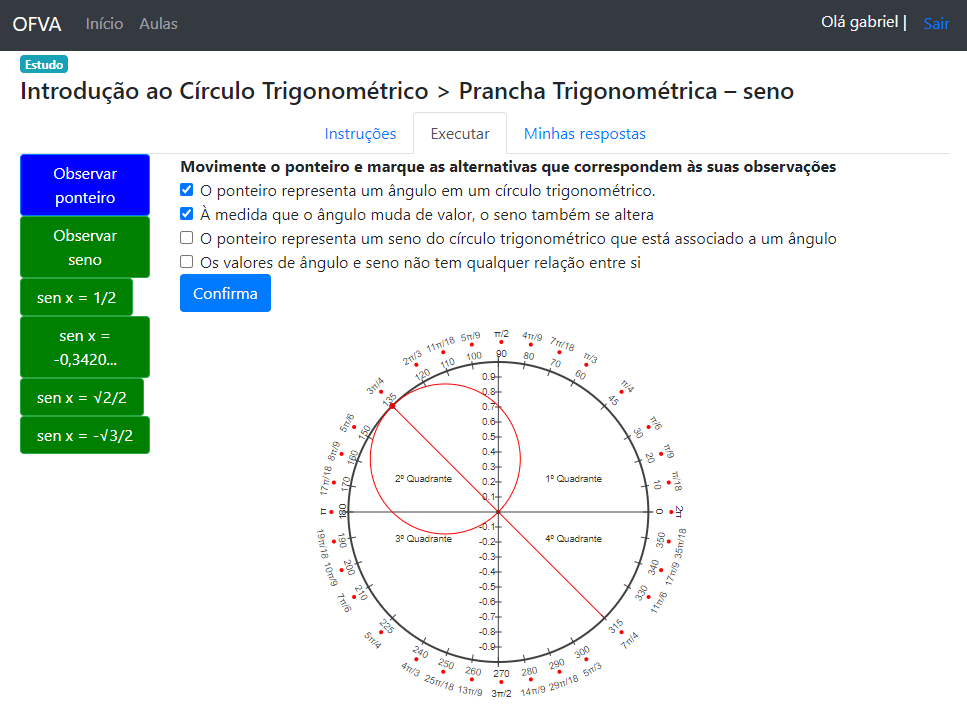
\includegraphics[width=0.9\linewidth]{chapters/results/Fase 3/E3_Virtual.png}
	\caption{Exercício 3 - Seno}
	\label{fig:E3}
\end{figure}

Além disso, é importante notar que este exercício implementa um objeto tangível com a terceira questão do exercício de fixação tradicional apresentado na Seção~\ref{section:atividade2_fixação}.

\textbf{Nota Tradicional - $NT$}

Conforme explicado anteriormente, o modo utilizado para a coleta de dados (`modo estudo') proporciona um caminho de construção do ciclo trigonométrico, de forma que é esperada a execução e a finalização da atividade a partir de orientações que o estudante recebe automaticamente da plataforma. No caso da nota tradicional, tanto o `modo estudo' quanto o `modo avaliação' utilizam as últimas respostas dadas pelo estudantes, consequentemente, não havendo diferença entre os resultados obtidos para as duas formas de cálculo e, além disso, quando a Nota Tradicional corresponde a $10.00$ é porque a atividade foi finalizada.

\begin{table}[htbp]
	\centering
	\caption{$NT$ - Nota Tradicional}
	\begin{tabular}{|c|c|c|c|c|c|c|c|}
		\hline
		\rowcolor[HTML]{D9D9D9} 
		\cellcolor[HTML]{D0CECE}\textbf{Participante} & \textbf{C1} & \textbf{C2} & \textbf{C3} & \textbf{C4} & \textbf{C5} & \textbf{C6} & \textbf{NT} \\ \hline
		\textbf{B02}     & 0.00  & 0.00  & 10.00 & 10.00 & 10.00 & 10.00 & 6.667  \\ \hline
		\rowcolor[HTML]{F2F2F2} 
		\textbf{B03}     & 10.00 & 10.00 & 10.00 & 10.00 & 10.00 & 10.00 & 10.000 \\ \hline
		\textbf{B04}     & 10.00 & 0.00  & 10.00 & 10.00 & 10.00 & 10.00 & 8.333  \\ \hline
		\rowcolor[HTML]{F2F2F2} 
		\textbf{B05}     & 10.00 & 0.00  & 10.00 & 10.00 & 10.00 & 10.00 & 8.333  \\ \hline
		\textbf{B06}     & 10.00 & 0.00  & 10.00 & 10.00 & 10.00 & 10.00 & 8.333  \\ \hline
		\rowcolor[HTML]{F2F2F2} 
		\textbf{B08}     & 10.00 & 10.00 & 10.00 & 10.00 & 10.00 & 10.00 & 10.000 \\ \hline
		\textbf{B09}     & 10.00 & 10.00 & 10.00 & 10.00 & 10.00 & 10.00 & 10.000 \\ \hline
		\rowcolor[HTML]{EFEFEF} 
		\textbf{B10}     & 10.00 & 0.00  & 10.00 & 10.00 & 10.00 & 10.00 & 8.333  \\ \hline
		\rowcolor[HTML]{D0CECE} 
		\textbf{NT Casos} & 8.75  & 3.75  & 10.00 & 10.00 & 10.00 & 10.00 & 8.750   \\ \hline
	\end{tabular}
	\label{tab:F3_A3_NT}
\end{table}

Assim, pode-se notar que somente os participantes $B03$, $B08$ e $B09$ finalizaram toda a atividades, enquanto o participante $B02$ não finalizou o caso de teste $C1$, $B04$, $B05$, $B06$ e $B10$ não finalizaram o caso $C2$. De modo que, inicialmente, é possível considerar que o $C2$ foi a questão em que os participantes tiveram maior dificuldade. Salienta-se que o caso de teste $C2$ prevê a observação da reta dos senos de modo que algumas características possam ser percebidas e enunciadas pelos estudantes. 

Com esta métrica mais tradicional, as possibilidades de acompanhamento são mais limitadas, uma vez que a nota tradicional é calculada com base na última resposta enviada pelo participante.

\textbf{Nota Ponderada - $NP$}

Com relação à Nota Ponderada, a Tabela~\ref{tab:F3_A3_NP_ESTUDO} apresenta os dados calculados utilizando o `modo estudo', enquanto a Tabela~\ref{tab:F3_A3_NP_AVALIACAO} faz um adendo a esta análise através do cálculo utilizado para o `modo avaliação'. 

É importante ressaltar que o modo `estudo' utiliza a média dos pesos obtidos por cada resposta enviada pelo participante de modo que o resultado final do cálculo tende a refletir (na média) o caminho do estudante. Assim, quanto maior a nota ponderada, as diversas respostas submetidas pelo participantes estão mais próximas da resposta correta. Ademais, o cálculo utilizado pelo modo `avaliação', assim como a Nota Tradicional, leva em consideração somente a última resposta enviada.

Observando-se a Tabela~\ref{tab:F3_A3_NP_ESTUDO}, nota-se que os participantes $B04$ e $B06$ obtiveram os menores valores, respectivamente, $4.699$ e $4.369$, entretanto, somente dois participantes ($B08$ e $B09$) obtiveram $NP$ acima de $70\%$, indicando uma possível dificuldade do grupo em realizar a atividade.

\begin{table}[htbp]
	\centering
	\caption{$NP$ - Nota Ponderada - Estudo}
	\begin{tabular}{|c|ccccccc|}
		\hline
		\rowcolor[HTML]{D0CECE} 
		\cellcolor[HTML]{D0CECE} &
		\multicolumn{7}{c|}{\cellcolor[HTML]{D0CECE}\textbf{Casos   de Teste}} \\ \cline{2-8} 
		\rowcolor[HTML]{D9D9D9} 
		\multirow{-2}{*}{\cellcolor[HTML]{D0CECE}\textbf{Participante}} &
		\multicolumn{1}{c|}{\cellcolor[HTML]{D9D9D9}\textbf{C1}} &
		\multicolumn{1}{c|}{\cellcolor[HTML]{D9D9D9}\textbf{C2}} &
		\multicolumn{1}{c|}{\cellcolor[HTML]{D9D9D9}\textbf{C3}} &
		\multicolumn{1}{c|}{\cellcolor[HTML]{D9D9D9}\textbf{C4}} &
		\multicolumn{1}{c|}{\cellcolor[HTML]{D9D9D9}\textbf{C5}} &
		\multicolumn{1}{c|}{\cellcolor[HTML]{D9D9D9}\textbf{C6}} &
		\textbf{NP} \\ \hline
		\textbf{B02} &
		\multicolumn{1}{c|}{\cellcolor[HTML]{FFFFFF}0.00} &
		\multicolumn{1}{c|}{\cellcolor[HTML]{FFFFFF}2.64} &
		\multicolumn{1}{c|}{\cellcolor[HTML]{FFFFFF}10.00} &
		\multicolumn{1}{c|}{\cellcolor[HTML]{FFFFFF}10.00} &
		\multicolumn{1}{c|}{\cellcolor[HTML]{FFFFFF}10.00} &
		\multicolumn{1}{c|}{\cellcolor[HTML]{FFFFFF}2.00} &
		5.773 \\ \hline
		\rowcolor[HTML]{F2F2F2} 
		\textbf{B03} &
		\multicolumn{1}{c|}{\cellcolor[HTML]{F2F2F2}5.83} &
		\multicolumn{1}{c|}{\cellcolor[HTML]{F2F2F2}8.75} &
		\multicolumn{1}{c|}{\cellcolor[HTML]{F2F2F2}2.92} &
		\multicolumn{1}{c|}{\cellcolor[HTML]{F2F2F2}4.50} &
		\multicolumn{1}{c|}{\cellcolor[HTML]{F2F2F2}2.50} &
		\multicolumn{1}{c|}{\cellcolor[HTML]{F2F2F2}6.25} &
		5.125 \\ \hline
		\textbf{B04} &
		\multicolumn{1}{c|}{\cellcolor[HTML]{FFFFFF}5.00} &
		\multicolumn{1}{c|}{\cellcolor[HTML]{FFFFFF}6.25} &
		\multicolumn{1}{c|}{\cellcolor[HTML]{FFFFFF}1.67} &
		\multicolumn{1}{c|}{\cellcolor[HTML]{FFFFFF}2.50} &
		\multicolumn{1}{c|}{\cellcolor[HTML]{FFFFFF}2.78} &
		\multicolumn{1}{c|}{\cellcolor[HTML]{FFFFFF}10.00} &
		4.699 \\ \hline
		\rowcolor[HTML]{F2F2F2} 
		\textbf{B05} &
		\multicolumn{1}{c|}{\cellcolor[HTML]{F2F2F2}8.75} &
		\multicolumn{1}{c|}{\cellcolor[HTML]{F2F2F2}3.82} &
		\multicolumn{1}{c|}{\cellcolor[HTML]{F2F2F2}3.33} &
		\multicolumn{1}{c|}{\cellcolor[HTML]{F2F2F2}10.00} &
		\multicolumn{1}{c|}{\cellcolor[HTML]{F2F2F2}2.92} &
		\multicolumn{1}{c|}{\cellcolor[HTML]{F2F2F2}7.50} &
		6.053 \\ \hline
		\textbf{B06} &
		\multicolumn{1}{c|}{\cellcolor[HTML]{FFFFFF}1.11} &
		\multicolumn{1}{c|}{\cellcolor[HTML]{FFFFFF}4.32} &
		\multicolumn{1}{c|}{\cellcolor[HTML]{FFFFFF}10.00} &
		\multicolumn{1}{c|}{\cellcolor[HTML]{FFFFFF}1.94} &
		\multicolumn{1}{c|}{\cellcolor[HTML]{FFFFFF}5.63} &
		\multicolumn{1}{c|}{\cellcolor[HTML]{FFFFFF}3.21} &
		4.369 \\ \hline
		\rowcolor[HTML]{F2F2F2} 
		\textbf{B08} &
		\multicolumn{1}{c|}{\cellcolor[HTML]{F2F2F2}10.00} &
		\multicolumn{1}{c|}{\cellcolor[HTML]{F2F2F2}6.88} &
		\multicolumn{1}{c|}{\cellcolor[HTML]{F2F2F2}10.00} &
		\multicolumn{1}{c|}{\cellcolor[HTML]{F2F2F2}2.92} &
		\multicolumn{1}{c|}{\cellcolor[HTML]{F2F2F2}10.00} &
		\multicolumn{1}{c|}{\cellcolor[HTML]{F2F2F2}7.50} &
		7.882 \\ \hline
		\textbf{B09} &
		\multicolumn{1}{c|}{\cellcolor[HTML]{FFFFFF}10.00} &
		\multicolumn{1}{c|}{\cellcolor[HTML]{FFFFFF}4.21} &
		\multicolumn{1}{c|}{\cellcolor[HTML]{FFFFFF}10.00} &
		\multicolumn{1}{c|}{\cellcolor[HTML]{FFFFFF}5.00} &
		\multicolumn{1}{c|}{\cellcolor[HTML]{FFFFFF}10.00} &
		\multicolumn{1}{c|}{\cellcolor[HTML]{FFFFFF}3.86} &
		7.179 \\ \hline
		\rowcolor[HTML]{F2F2F2} 
		\textbf{B10} &
		\multicolumn{1}{c|}{\cellcolor[HTML]{F2F2F2}3.33} &
		\multicolumn{1}{c|}{\cellcolor[HTML]{F2F2F2}0.00} &
		\multicolumn{1}{c|}{\cellcolor[HTML]{F2F2F2}5.00} &
		\multicolumn{1}{c|}{\cellcolor[HTML]{F2F2F2}7.50} &
		\multicolumn{1}{c|}{\cellcolor[HTML]{F2F2F2}10.00} &
		\multicolumn{1}{c|}{\cellcolor[HTML]{F2F2F2}10.00} &
		5.972 \\ \hline
		\rowcolor[HTML]{D0CECE} 
		\textbf{NP Casos} &
		\multicolumn{1}{c|}{\cellcolor[HTML]{D0CECE}5.50} &
		\multicolumn{1}{c|}{\cellcolor[HTML]{D0CECE}4.61} &
		\multicolumn{1}{c|}{\cellcolor[HTML]{D0CECE}6.61} &
		\multicolumn{1}{c|}{\cellcolor[HTML]{D0CECE}5.55} &
		\multicolumn{1}{c|}{\cellcolor[HTML]{D0CECE}6.73} &
		\multicolumn{1}{c|}{\cellcolor[HTML]{D0CECE}6.29} &
		5.881 \\ \hline
	\end{tabular}
	\label{tab:F3_A3_NP_ESTUDO}
\end{table}

Além disso, os casos de teste com menor desempenho do grupo foram $C2$ e $C1$, respectivamente, onde os valores obtidos foram $4.61$ e $5.50$. Além disso, tais casos de teste correspondem a questões relacionadas a observação da relação dos ângulos com o seno, de modo que esse é um indicativo inicial de que esses casos são mais difíceis do que os demais e que, por isso, os participantes tiveram maior dificuldade.

É importante ressaltar que, diferentemente dos Exercícios 1 e 2, neste exercício as métricas não foram calculadas considerando as entradas, uma vez que para os casos de teste $C3$ a $C5$ há somente a entrada física $EF1$. Ademais, para os casos de teste $C1$ e $C2$ pode haver mais de uma entrada virtual correta, de modo que a correção do caso de teste considerando os pesos apresentados no modelo proposto obedece a lógica definida nas tabelas do Apêndice~\ref{Chap:AppendixAnaliticosA03}.

\begin{table}[htbp]
	\centering
	\caption{$NP$ - Nota Ponderada - Avaliação}
	\begin{tabular}{|c|ccccccc|}
		\hline
		\rowcolor[HTML]{D0CECE} 
		\cellcolor[HTML]{D0CECE} &
		\multicolumn{7}{c|}{\cellcolor[HTML]{D0CECE}\textbf{Casos de Teste}} \\ \cline{2-8} 
		\rowcolor[HTML]{D9D9D9} 
		\multirow{-2}{*}{\cellcolor[HTML]{D0CECE}\textbf{Participante}} &
		\multicolumn{1}{c|}{\cellcolor[HTML]{D9D9D9}\textbf{C1}} &
		\multicolumn{1}{c|}{\cellcolor[HTML]{D9D9D9}\textbf{C2}} &
		\multicolumn{1}{c|}{\cellcolor[HTML]{D9D9D9}\textbf{C3}} &
		\multicolumn{1}{c|}{\cellcolor[HTML]{D9D9D9}\textbf{C4}} &
		\multicolumn{1}{c|}{\cellcolor[HTML]{D9D9D9}\textbf{C5}} &
		\multicolumn{1}{c|}{\cellcolor[HTML]{D9D9D9}\textbf{C6}} &
		\textbf{Média} \\ \hline
		\textbf{B02} &
		\multicolumn{1}{c|}{\cellcolor[HTML]{FFFFFF}0.00} &
		\multicolumn{1}{c|}{\cellcolor[HTML]{FFFFFF}7.50} &
		\multicolumn{1}{c|}{\cellcolor[HTML]{FFFFFF}10.00} &
		\multicolumn{1}{c|}{\cellcolor[HTML]{FFFFFF}10.00} &
		\multicolumn{1}{c|}{\cellcolor[HTML]{FFFFFF}10.00} &
		\multicolumn{1}{c|}{\cellcolor[HTML]{FFFFFF}10.00} &
		7.917 \\ \hline
		\rowcolor[HTML]{F2F2F2} 
		\textbf{B03} &
		\multicolumn{1}{c|}{\cellcolor[HTML]{F2F2F2}10.00} &
		\multicolumn{1}{c|}{\cellcolor[HTML]{F2F2F2}10.00} &
		\multicolumn{1}{c|}{\cellcolor[HTML]{F2F2F2}10.00} &
		\multicolumn{1}{c|}{\cellcolor[HTML]{F2F2F2}10.00} &
		\multicolumn{1}{c|}{\cellcolor[HTML]{F2F2F2}10.00} &
		\multicolumn{1}{c|}{\cellcolor[HTML]{F2F2F2}10.00} &
		10.000 \\ \hline
		\textbf{B04} &
		\multicolumn{1}{c|}{\cellcolor[HTML]{FFFFFF}10.00} &
		\multicolumn{1}{c|}{\cellcolor[HTML]{FFFFFF}5.00} &
		\multicolumn{1}{c|}{\cellcolor[HTML]{FFFFFF}10.00} &
		\multicolumn{1}{c|}{\cellcolor[HTML]{FFFFFF}10.00} &
		\multicolumn{1}{c|}{\cellcolor[HTML]{FFFFFF}10.00} &
		\multicolumn{1}{c|}{\cellcolor[HTML]{FFFFFF}10.00} &
		9.167 \\ \hline
		\rowcolor[HTML]{F2F2F2} 
		\textbf{B05} &
		\multicolumn{1}{c|}{\cellcolor[HTML]{F2F2F2}10.00} &
		\multicolumn{1}{c|}{\cellcolor[HTML]{F2F2F2}2.50} &
		\multicolumn{1}{c|}{\cellcolor[HTML]{F2F2F2}10.00} &
		\multicolumn{1}{c|}{\cellcolor[HTML]{F2F2F2}10.00} &
		\multicolumn{1}{c|}{\cellcolor[HTML]{F2F2F2}10.00} &
		\multicolumn{1}{c|}{\cellcolor[HTML]{F2F2F2}10.00} &
		8.750 \\ \hline
		\textbf{B06} &
		\multicolumn{1}{c|}{\cellcolor[HTML]{FFFFFF}10.00} &
		\multicolumn{1}{c|}{\cellcolor[HTML]{FFFFFF}7.50} &
		\multicolumn{1}{c|}{\cellcolor[HTML]{FFFFFF}10.00} &
		\multicolumn{1}{c|}{\cellcolor[HTML]{FFFFFF}10.00} &
		\multicolumn{1}{c|}{\cellcolor[HTML]{FFFFFF}10.00} &
		\multicolumn{1}{c|}{\cellcolor[HTML]{FFFFFF}10.00} &
		9.583 \\ \hline
		\rowcolor[HTML]{F2F2F2} 
		\textbf{B08} &
		\multicolumn{1}{c|}{\cellcolor[HTML]{F2F2F2}10.00} &
		\multicolumn{1}{c|}{\cellcolor[HTML]{F2F2F2}10.00} &
		\multicolumn{1}{c|}{\cellcolor[HTML]{F2F2F2}10.00} &
		\multicolumn{1}{c|}{\cellcolor[HTML]{F2F2F2}10.00} &
		\multicolumn{1}{c|}{\cellcolor[HTML]{F2F2F2}10.00} &
		\multicolumn{1}{c|}{\cellcolor[HTML]{F2F2F2}10.00} &
		10.000 \\ \hline
		\textbf{B09} &
		\multicolumn{1}{c|}{\cellcolor[HTML]{FFFFFF}10.00} &
		\multicolumn{1}{c|}{\cellcolor[HTML]{FFFFFF}10.00} &
		\multicolumn{1}{c|}{\cellcolor[HTML]{FFFFFF}10.00} &
		\multicolumn{1}{c|}{\cellcolor[HTML]{FFFFFF}10.00} &
		\multicolumn{1}{c|}{\cellcolor[HTML]{FFFFFF}10.00} &
		\multicolumn{1}{c|}{\cellcolor[HTML]{FFFFFF}10.00} &
		10.000 \\ \hline
		\rowcolor[HTML]{F2F2F2} 
		\textbf{B10} &
		\multicolumn{1}{c|}{\cellcolor[HTML]{F2F2F2}10.00} &
		\multicolumn{1}{c|}{\cellcolor[HTML]{F2F2F2}0.00} &
		\multicolumn{1}{c|}{\cellcolor[HTML]{F2F2F2}10.00} &
		\multicolumn{1}{c|}{\cellcolor[HTML]{F2F2F2}10.00} &
		\multicolumn{1}{c|}{\cellcolor[HTML]{F2F2F2}10.00} &
		\multicolumn{1}{c|}{\cellcolor[HTML]{F2F2F2}10.00} &
		8.333 \\ \hline
		\rowcolor[HTML]{D0CECE} 
		\textbf{Média} &
		\multicolumn{1}{c|}{\cellcolor[HTML]{D0CECE}8.75} &
		\multicolumn{1}{c|}{\cellcolor[HTML]{D0CECE}6.56} &
		\multicolumn{1}{c|}{\cellcolor[HTML]{D0CECE}10.00} &
		\multicolumn{1}{c|}{\cellcolor[HTML]{D0CECE}10.00} &
		\multicolumn{1}{c|}{\cellcolor[HTML]{D0CECE}10.00} &
		\multicolumn{1}{c|}{\cellcolor[HTML]{D0CECE}10.00} &
		9.219 \\ \hline
	\end{tabular}
	\label{tab:F3_A3_NP_AVALIACAO}
\end{table}

Ao observar os valores da Tabela~\ref{tab:F3_A3_NP_AVALIACAO}, nota-se que os participantes $B02$ e $B10$ realmente responderam incorretamente os casos de teste $C1$ e $C2$, respectivamente, uma vez que $NP$ é igual a zero para ambos. Com relação a $C2$, nota-se que, embora a Nota Tradicional indique que os participantes $B02$ e $B06$ erraram totalmente a questão, a resposta dada por eles foi muito próxima ao correto, uma vez que a $NP$ de ambos é $7.50$.

\textbf{Prioridade - $P$}

\begin{table}[htbp]
	\centering
	\caption{$P$ - Prioridade}
	\begin{tabular}{|c|ccccccc|}
		\hline
		\rowcolor[HTML]{D0CECE} 
		\cellcolor[HTML]{D0CECE} & \multicolumn{7}{c|}{\cellcolor[HTML]{D0CECE}\textbf{Casos de Teste}} \\ \cline{2-8} 
		\rowcolor[HTML]{D9D9D9} 
		\multirow{-2}{*}{\cellcolor[HTML]{D0CECE}\textbf{Participante}} & \multicolumn{1}{c|}{\cellcolor[HTML]{D9D9D9}\textbf{C1}} & \multicolumn{1}{c|}{\cellcolor[HTML]{D9D9D9}\textbf{C2}} & \multicolumn{1}{c|}{\cellcolor[HTML]{D9D9D9}\textbf{C3}} & \multicolumn{1}{c|}{\cellcolor[HTML]{D9D9D9}\textbf{C4}} & \multicolumn{1}{c|}{\cellcolor[HTML]{D9D9D9}\textbf{C5}} & \multicolumn{1}{c|}{\cellcolor[HTML]{D9D9D9}\textbf{C6}} & \textbf{P} \\ \hline
		\textbf{B02} & \multicolumn{1}{c|}{0.00} & \multicolumn{1}{c|}{2.64} & \multicolumn{1}{c|}{0.00} & \multicolumn{1}{c|}{0.00} & \multicolumn{1}{c|}{0.00} & \multicolumn{1}{c|}{0.00} & 1.924 \\ \hline
		\rowcolor[HTML]{F2F2F2} 
		\textbf{B03} & \multicolumn{1}{c|}{\cellcolor[HTML]{F2F2F2}0.00} & \multicolumn{1}{c|}{\cellcolor[HTML]{F2F2F2}0.00} & \multicolumn{1}{c|}{\cellcolor[HTML]{F2F2F2}0.00} & \multicolumn{1}{c|}{\cellcolor[HTML]{F2F2F2}0.00} & \multicolumn{1}{c|}{\cellcolor[HTML]{F2F2F2}0.00} & \multicolumn{1}{c|}{\cellcolor[HTML]{F2F2F2}0.00} & 0.000 \\ \hline
		\textbf{B04} & \multicolumn{1}{c|}{0.00} & \multicolumn{1}{c|}{6.25} & \multicolumn{1}{c|}{0.00} & \multicolumn{1}{c|}{0.00} & \multicolumn{1}{c|}{0.00} & \multicolumn{1}{c|}{0.00} & 0.783 \\ \hline
		\rowcolor[HTML]{F2F2F2} 
		\textbf{B05} & \multicolumn{1}{c|}{\cellcolor[HTML]{F2F2F2}0.00} & \multicolumn{1}{c|}{\cellcolor[HTML]{F2F2F2}3.82} & \multicolumn{1}{c|}{\cellcolor[HTML]{F2F2F2}0.00} & \multicolumn{1}{c|}{\cellcolor[HTML]{F2F2F2}0.00} & \multicolumn{1}{c|}{\cellcolor[HTML]{F2F2F2}0.00} & \multicolumn{1}{c|}{\cellcolor[HTML]{F2F2F2}0.00} & 1.009 \\ \hline
		\textbf{B06} & \multicolumn{1}{c|}{0.00} & \multicolumn{1}{c|}{4.32} & \multicolumn{1}{c|}{0.00} & \multicolumn{1}{c|}{0.00} & \multicolumn{1}{c|}{0.00} & \multicolumn{1}{c|}{0.00} & 0.728 \\ \hline
		\rowcolor[HTML]{F2F2F2} 
		\textbf{B08} & \multicolumn{1}{c|}{\cellcolor[HTML]{F2F2F2}0.00} & \multicolumn{1}{c|}{\cellcolor[HTML]{F2F2F2}0.00} & \multicolumn{1}{c|}{\cellcolor[HTML]{F2F2F2}0.00} & \multicolumn{1}{c|}{\cellcolor[HTML]{F2F2F2}0.00} & \multicolumn{1}{c|}{\cellcolor[HTML]{F2F2F2}0.00} & \multicolumn{1}{c|}{\cellcolor[HTML]{F2F2F2}0.00} & 0.000 \\ \hline
		\textbf{B09} & \multicolumn{1}{c|}{0.00} & \multicolumn{1}{c|}{0.00} & \multicolumn{1}{c|}{0.00} & \multicolumn{1}{c|}{0.00} & \multicolumn{1}{c|}{0.00} & \multicolumn{1}{c|}{0.00} & 0.000 \\ \hline
		\rowcolor[HTML]{F2F2F2} 
		\textbf{B10} & \multicolumn{1}{c|}{\cellcolor[HTML]{F2F2F2}0.00} & \multicolumn{1}{c|}{\cellcolor[HTML]{F2F2F2}0.00} & \multicolumn{1}{c|}{\cellcolor[HTML]{F2F2F2}0.00} & \multicolumn{1}{c|}{\cellcolor[HTML]{F2F2F2}0.00} & \multicolumn{1}{c|}{\cellcolor[HTML]{F2F2F2}0.00} & \multicolumn{1}{c|}{\cellcolor[HTML]{F2F2F2}0.00} & 0.995 \\ \hline
		\rowcolor[HTML]{D0CECE} 
		\textbf{P Casos} & \multicolumn{1}{c|}{\cellcolor[HTML]{D0CECE}0.00} & \multicolumn{1}{c|}{\cellcolor[HTML]{D0CECE}2.13} & \multicolumn{1}{c|}{\cellcolor[HTML]{D0CECE}0.00} & \multicolumn{1}{c|}{\cellcolor[HTML]{D0CECE}0.00} & \multicolumn{1}{c|}{\cellcolor[HTML]{D0CECE}0.00} & \multicolumn{1}{c|}{\cellcolor[HTML]{D0CECE}0.00} & 0.680 \\ \hline
	\end{tabular}
	\label{tab:F3_A3_P}
\end{table}

Com relação à prioridade, de acordo com a Tabela~\ref{tab:F3_A3_P}, os participantes $B03$, $B08$ e $B09$ apresentaram resultados iguais a zero, uma vez que, de acordo com a Equação~\ref{eq:prioridade}, esta métrica depende de os valores de $NT$ e $NP$ serem diferentes de $10$ e de $0$, respectivamente. 

Ressalta-se o participante $B10$ que, apesar de ter tido prioridade igual a zero para todos os casos de teste individualmente, obteve a terceira maior prioridade do grupo. Isso aconteceu por influência das notas tradicional e ponderada que ele obteve para o exercício, uma vez que a prioridade geral do participante é calculada com base nos valores das métricas para o exercício.

Considerando o exercício como um todo, o participante com maior prioridade de acompanhamento é $B02$, cujo valor obtido foi de $1.924$, seguido por $B05$ com prioridade igual a $1.009$.

Além disso, também foi possível calcular a prioridade para os participantes $B02$, $B04$, $B05$ e $B06$ para o caso $C2$, devido aos valores de $NT$ e $NP$ obtidos neste caso de teste. Ainda ao observar o mesmo caso de teste, nota-se que o participante com maior prioridade é $B04$, seguido por $B06$ e $B05$, de modo que esta ordem pode indicar participantes com necessidade de um acompanhamento mais próximo por parte do professor.

\textbf{Dúvida - $D$}

A Tabela~\ref{tab:F3_A3_DUVIDA} apresenta os valores de Dúvida dos participantes, onde os três que obtiveram maior valor foram $B02$, $B06$ e $B09$ cujos valores absolutos são $38$, $35$ e $29$, respectivamente. Além destes, os participantes $B04$ e $B05$, cujos valores são $24$ e $27$, também obtiveram uma dúvida absoluta maior do que a média do grupo $22.63$.

\begin{table}[htbp]
	\centering
	\caption{$D$ - Dúvida}
	\begin{tabular}{|c|c|c|c|c|c|c|ccc}
		\hline
		\rowcolor[HTML]{D9D9D9} 
		\cellcolor[HTML]{D0CECE}\textbf{Participante} & \textbf{C1} & \textbf{C2} & \textbf{C3} & \textbf{C4} & \textbf{C5} & \textbf{C6} & \multicolumn{1}{c|}{\cellcolor[HTML]{D9D9D9}\textbf{Total}} & \multicolumn{1}{c|}{\cellcolor[HTML]{D9D9D9}\textbf{Média}} & \multicolumn{1}{c|}{\cellcolor[HTML]{D9D9D9}\textbf{DP}} \\ \hline
		\cellcolor[HTML]{F2F2F2}\textbf{B02} & -1 & 35 & 0 & 0 & 0 & 4 & \multicolumn{1}{c|}{38} & \multicolumn{1}{c|}{6.33} & \multicolumn{1}{c|}{14.15} \\ \hline
		\rowcolor[HTML]{D9D9D9} 
		\cellcolor[HTML]{F2F2F2}\textbf{B03} & 2 & 1 & 5 & 4 & 3 & 1 & \multicolumn{1}{c|}{\cellcolor[HTML]{D9D9D9}16} & \multicolumn{1}{c|}{\cellcolor[HTML]{D9D9D9}2.67} & \multicolumn{1}{c|}{\cellcolor[HTML]{D9D9D9}1.63} \\ \hline
		\cellcolor[HTML]{F2F2F2}\textbf{B04} & 1 & 3 & 5 & 7 & 8 & 0 & \multicolumn{1}{c|}{24} & \multicolumn{1}{c|}{4.00} & \multicolumn{1}{c|}{3.22} \\ \hline
		\rowcolor[HTML]{D9D9D9} 
		\cellcolor[HTML]{F2F2F2}\textbf{B05} & 1 & 15 & 5 & 0 & 5 & 1 & \multicolumn{1}{c|}{\cellcolor[HTML]{D9D9D9}27} & \multicolumn{1}{c|}{\cellcolor[HTML]{D9D9D9}4.50} & \multicolumn{1}{c|}{\cellcolor[HTML]{D9D9D9}5.58} \\ \hline
		\cellcolor[HTML]{F2F2F2}\textbf{B06} & 8 & 10 & 0 & 8 & 3 & 6 & \multicolumn{1}{c|}{35} & \multicolumn{1}{c|}{5.83} & \multicolumn{1}{c|}{3.71} \\ \hline
		\rowcolor[HTML]{D9D9D9} 
		\cellcolor[HTML]{F2F2F2}\textbf{B08} & 0 & 3 & 0 & 5 & 0 & 1 & \multicolumn{1}{c|}{\cellcolor[HTML]{D9D9D9}9} & \multicolumn{1}{c|}{\cellcolor[HTML]{D9D9D9}1.50} & \multicolumn{1}{c|}{\cellcolor[HTML]{D9D9D9}2.07} \\ \hline
		\cellcolor[HTML]{F2F2F2}\textbf{B09} & 0 & 18 & 0 & 1 & 0 & 10 & \multicolumn{1}{c|}{29} & \multicolumn{1}{c|}{4.83} & \multicolumn{1}{c|}{7.55} \\ \hline
		\rowcolor[HTML]{D9D9D9} 
		\cellcolor[HTML]{F2F2F2}\textbf{B10} & 2 & -1 & 1 & 1 & 0 & 0 & \multicolumn{1}{c|}{\cellcolor[HTML]{D9D9D9}3} & \multicolumn{1}{c|}{\cellcolor[HTML]{D9D9D9}0.50} & \multicolumn{1}{c|}{\cellcolor[HTML]{D9D9D9}1.05} \\ \hline
		\textbf{Dúvida Caso} & 1.63 & 10.50 & 2.00 & 3.25 & 2.38 & 2.88 & \multicolumn{1}{c|}{22.63} & \multicolumn{1}{l}{} & \multicolumn{1}{l}{} \\ \cline{1-8}
		\cellcolor[HTML]{D9D9D9}\textbf{Desvio-Padrão} & \cellcolor[HTML]{D9D9D9}2.77 & \cellcolor[HTML]{D9D9D9}12.02 & \cellcolor[HTML]{D9D9D9}2.51 & \cellcolor[HTML]{D9D9D9}3.20 & \cellcolor[HTML]{D9D9D9}2.97 & \cellcolor[HTML]{D9D9D9}3.56 & \multicolumn{1}{l}{} & \multicolumn{1}{l}{} & \multicolumn{1}{l}{} \\ \cline{1-7}
	\end{tabular}
	\label{tab:F3_A3_DUVIDA}
\end{table}

Embora o valor calculado como `Dúvida Média' siga o mesmo padrão/proporção do absoluto da Dúvida, ele pode auxiliar em uma percepção com relação ao todo do exercício, considerando a existência de diversos casos de teste. Além disso, quando associado ao desvio-padrão, pode-se inferir se a distribuição da dúvida nos casos de teste foi homogênea ou não. Assim, ao observar que o desvio-padrão do participante $B02$ é muito elevado, é possível verificar que, embora a Dúvida e a Média da Dúvida de $B02$ sejam os mais elevados do grupo, esse valor foi impulsionado tão somente por um único caso de teste ($C2$), enquanto os valores dos casos de teste restantes são mais baixos.

Outro exemplo a ser destacado é o participante $B06$, cuja média foi de $5.83$ e desvio-padrão de $3.71$. Embora sua média seja a mais próxima de $B02$, seu desvio padrão está muito abaixo, indicando que a distribuição da Dúvida deste participante é mais homogênea e, logo, alterou mais consistentemente uma maior quantidade de casos de teste.

Com relação aos casos de teste, os três casos com menor dúvida foram $C1$, $C3$ e $C5$, tendo uma média de $1.63$, $2.00$ e $2.38$. Destes casos, $C3$ tem o menor desvio-padrão, de modo que é o caso com a distribuição de valores mais homogênea, seguido por $C1$ e $C5$, respectivamente.

É importante destacar que o caso $C2$ obteve dúvida de $10.50$ com um desvio-padrão $12.02$, sendo ambos os maiores valores entre os casos utilizados no exercício. Esse elevado desvio-padrão é resultado do fato de que a média foi impulsionada para cima somente pelo participante $B02$, cuja dúvida foi igual a $35$. Por fim, os participantes $B02$ e $B10$ obtiveram o valor $-1$ nos casos $C1$ e $C2$, respectivamente, indicando que ambos não responderam a esses casos de teste.

\textbf{Assertividade - $A$}

Os valores de Assertividade são mostrados na Tabela~\ref{tab:F3_A3_A}, de modo que é possível notar que os três participantes com menor percentual são $B02$, $B06$ e $B04$, onde os dois primeiros possuem uma assertividade abaixo de $10\%$ e o terceiro $16\%$. Além disso, estes são os três participantes com $A$ abaixo da média do grupo ($19\%$).

É importante notar que todos os participantes possuem valor de $A$ abaixo de $35\%$, de modo que o maior valor foi obtido por $B10$ correspondendo a $33\%$, seguido por $B03$ com $30\%$.

\begin{table}[htbp]
	\centering
	\caption{$A$ - Assertividade}
	\begin{tabular}{|c|c|c|c|c|c|c|c|}
		\hline
		\rowcolor[HTML]{D9D9D9} 
		\textbf{Participante} & \textbf{C1} & \textbf{C2} & \textbf{C3} & \textbf{C4} & \textbf{C5} & \textbf{C6} & \textbf{A} \\ \hline
		\textbf{B02} & 0.00 & 0.00 & 0.00 & 0.00 & 0.00 & 0.25 & 0.04 \\ \hline
		\rowcolor[HTML]{D9D9D9} 
		\textbf{B03} & 0.00 & 0.00 & 0.20 & 0.25 & 0.33 & 1.00 & 0.30 \\ \hline
		\textbf{B04} & 0.00 & 0.00 & 0.20 & 0.14 & 0.13 & 0.00 & 0.08 \\ \hline
		\rowcolor[HTML]{D9D9D9} 
		\textbf{B05} & 0.00 & 0.00 & 0.20 & 0.00 & 0.20 & 1.00 & 0.23 \\ \hline
		\textbf{B06} & 0.00 & 0.00 & 0.00 & 0.13 & 0.67 & 0.17 & 0.16 \\ \hline
		\rowcolor[HTML]{D9D9D9} 
		\textbf{B08} & 0.00 & 0.00 & 0.00 & 0.20 & 0.00 & 1.00 & 0.20 \\ \hline
		\textbf{B09} & 0.00 & 0.00 & 0.00 & 1.00 & 0.00 & 0.20 & 0.20 \\ \hline
		\rowcolor[HTML]{D9D9D9} 
		\textbf{B10} & 0.00 & 0.00 & 1.00 & 1.00 & 0.00 & 0.00 & 0.33 \\ \hline
		\textbf{A Casos} & 0.00 & 0.00 & 0.20 & 0.34 & 0.17 & 0.45 & 0.19 \\ \hline
	\end{tabular}
	\label{tab:F3_A3_A}
\end{table}

Com relação aos casos de teste, nota-se que casos $C1$ e $C2$ possuem os menores valores médios, correspondendo aos casos em que foi pedido aos participantes para manipularem o ponteiro físico à vontade de modo a observarem e indicarem a relação entre os valores dos ângulos e dos senos. 

O caso de teste com maior assertividade média foi $C6$ cujo valor de A é $45\%$. Além disso, os participantes $B03$, $B05$ e $B08$ obtiveram assertividade de $100\%$. Por fim, a Assertividade total do exercício foi de $19\%$.

\textbf{Níveis de Compreensão da Questão ($NCQ$) e do Questionário ($NC$)}

A Tabela~\ref{tab:F3_A3_NCQ} apresenta os valores de $NCQ$ e $NC$ para o Exercício 2, onde é possível notar que os participantes com menor desempenho da atividade são $B02$ e $B06$, cujos percentuais de Nível de Compreensão são $33\%$. Além disso, para ambos, o caso de teste com menor nível de compreensão da questão foi $C1$.

É interessante salientar que três participantes ($B08$, $B09$ e $B10$) obtiveram níveis de compreensão acima de $50\%$. Além disso, o participante $B08$ obtiveram o maior valor de $NC$, sendo $64\%$.

Ao observar o participante $B08$ (maior nível de compreensão), pode-se notar que teve mais dificuldade no caso de teste $C4$, cujo $NCQ$ é $13\%$. É interessante notar que, embora a Tabela~\ref{tab:F3_A3_NT} indique que o participante finalizou o caso de teste ($NT$ igual a $10.00$), a Tabela~\ref{tab:F3_A3_DUVIDA} indica uma dúvida absoluta igual a $5$, isto é, respondeu o caso de teste 6 vezes e a Tabela~\ref{tab:F3_A3_NP_ESTUDO} atribui uma nota ponderada igual a $2.92$ para este participante neste caso de teste (sendo a menor nota do participante no exercício).

\begin{table}[htbp]
	\centering
	\caption{$NCQ$ e $NC$}
	\begin{tabular}{|c|cccccc|c|}
		\hline
		\rowcolor[HTML]{D0CECE} 
		\cellcolor[HTML]{D9D9D9} & \multicolumn{6}{c|}{\cellcolor[HTML]{D0CECE}\textbf{NCQ}} & \cellcolor[HTML]{D9D9D9} \\ \cline{2-7}
		\rowcolor[HTML]{D9D9D9} 
		\multirow{-2}{*}{\cellcolor[HTML]{D9D9D9}\textbf{Participante}} & \multicolumn{1}{c|}{\cellcolor[HTML]{D9D9D9}\textbf{C1}} & \multicolumn{1}{c|}{\cellcolor[HTML]{D9D9D9}\textbf{C2}} & \multicolumn{1}{c|}{\cellcolor[HTML]{D9D9D9}\textbf{C3}} & \multicolumn{1}{c|}{\cellcolor[HTML]{D9D9D9}\textbf{C4}} & \multicolumn{1}{c|}{\cellcolor[HTML]{D9D9D9}\textbf{C5}} & \textbf{C6} & \multirow{-2}{*}{\cellcolor[HTML]{D9D9D9}\textbf{NC}} \\ \hline
		\textbf{B02} & \multicolumn{1}{c|}{0.00} & \multicolumn{1}{c|}{0.24} & \multicolumn{1}{c|}{0.53} & \multicolumn{1}{c|}{0.45} & \multicolumn{1}{c|}{0.83} & 0.18 & 0.33 \\ \hline
		\rowcolor[HTML]{D9D9D9} 
		\textbf{B03} & \multicolumn{1}{c|}{\cellcolor[HTML]{D9D9D9}0.58} & \multicolumn{1}{c|}{\cellcolor[HTML]{D9D9D9}0.88} & \multicolumn{1}{c|}{\cellcolor[HTML]{D9D9D9}0.19} & \multicolumn{1}{c|}{\cellcolor[HTML]{D9D9D9}0.33} & \multicolumn{1}{c|}{\cellcolor[HTML]{D9D9D9}0.24} & 0.63 & 0.42 \\ \hline
		\textbf{B04} & \multicolumn{1}{c|}{0.50} & \multicolumn{1}{c|}{0.63} & \multicolumn{1}{c|}{0.09} & \multicolumn{1}{c|}{0.12} & \multicolumn{1}{c|}{0.24} & 0.94 & 0.36 \\ \hline
		\rowcolor[HTML]{D9D9D9} 
		\textbf{B05} & \multicolumn{1}{c|}{\cellcolor[HTML]{D9D9D9}0.77} & \multicolumn{1}{c|}{\cellcolor[HTML]{D9D9D9}0.37} & \multicolumn{1}{c|}{\cellcolor[HTML]{D9D9D9}0.16} & \multicolumn{1}{c|}{\cellcolor[HTML]{D9D9D9}0.58} & \multicolumn{1}{c|}{\cellcolor[HTML]{D9D9D9}0.22} & 0.71 & 0.41 \\ \hline
		\textbf{B06} & \multicolumn{1}{c|}{0.10} & \multicolumn{1}{c|}{0.43} & \multicolumn{1}{c|}{0.80} & \multicolumn{1}{c|}{0.11} & \multicolumn{1}{c|}{0.52} & 0.31 & 0.33 \\ \hline
		\rowcolor[HTML]{D9D9D9} 
		\textbf{B08} & \multicolumn{1}{c|}{\cellcolor[HTML]{D9D9D9}0.95} & \multicolumn{1}{c|}{\cellcolor[HTML]{D9D9D9}0.69} & \multicolumn{1}{c|}{\cellcolor[HTML]{D9D9D9}0.85} & \multicolumn{1}{c|}{\cellcolor[HTML]{D9D9D9}0.13} & \multicolumn{1}{c|}{\cellcolor[HTML]{D9D9D9}0.99} & 0.75 & 0.64 \\ \hline
		\textbf{B09} & \multicolumn{1}{c|}{0.98} & \multicolumn{1}{c|}{0.41} & \multicolumn{1}{c|}{0.99} & \multicolumn{1}{c|}{0.30} & \multicolumn{1}{c|}{0.98} & 0.34 & 0.59 \\ \hline
		\rowcolor[HTML]{D9D9D9} 
		\textbf{B10} & \multicolumn{1}{c|}{\cellcolor[HTML]{D9D9D9}0.33} & \multicolumn{1}{c|}{\cellcolor[HTML]{D9D9D9}0.00} & \multicolumn{1}{c|}{\cellcolor[HTML]{D9D9D9}0.50} & \multicolumn{1}{c|}{\cellcolor[HTML]{D9D9D9}0.72} & \multicolumn{1}{c|}{\cellcolor[HTML]{D9D9D9}0.97} & 1.00 & 0.52 \\ \hline
		\textbf{Média} & \multicolumn{1}{c|}{0.53} & \multicolumn{1}{c|}{0.45} & \multicolumn{1}{c|}{0.51} & \multicolumn{1}{c|}{0.34} & \multicolumn{1}{c|}{0.62} & 0.61 & 0.45 \\ \hline
	\end{tabular}
	\label{tab:F3_A3_NCQ}
\end{table}

Os casos de teste com menor nível de compreensão foram $C4$ e $C2$, cujo percentual foi de $34\%$ e $45\%$\ respectivamente, de modo que estes são os únicos casos de teste com valor abaixo de $50\%$. Por fim, o percentual médio do nível de compreensão do exercício foi de $45\%$.

%Acerca dos casos de teste, os que obtiveram menor média do nível de compreensão da questão foram $C4$, cujo $NCQ$ foi $60\%$ e $C3$ com $NCQ$ igual a $73\%$, enquanto os casos de teste com maior média de $NCQ$ foram $61$ e $C1$ com valores de $96\%$ e $94\%$. Por fim, o $NC$ do exercício foi de $73\%$.

\subsubsection{Exercício 4 - Cosseno}\label{subsubsec:F3A4}

Conforme pode ser observado na Figura~\ref{fig:E4}, este exercício implementa a quarta questão da Atividade 2 (Seção~\ref{section:atividade2_fixação}), de modo que é abordado o conteúdo relacionado ao cosseno, onde os estudantes devem fazer observações a partir da manipulação do ponteiro físico para selecionar as afirmações corretas. 

A interface física utilizada nesta instância do objeto tangível é a A04 e sua imagem está disponível na Seção~\ref{subsection:atividade3_A04}, onde é possível observar o círculo trigonométrico parcialmente construído, contendo os quadrantes, todos os ângulos em graus e radianos, além do eixo dos cossenos, que é o objetivo da atividade.

\begin{figure}[!htb]
	\centering
	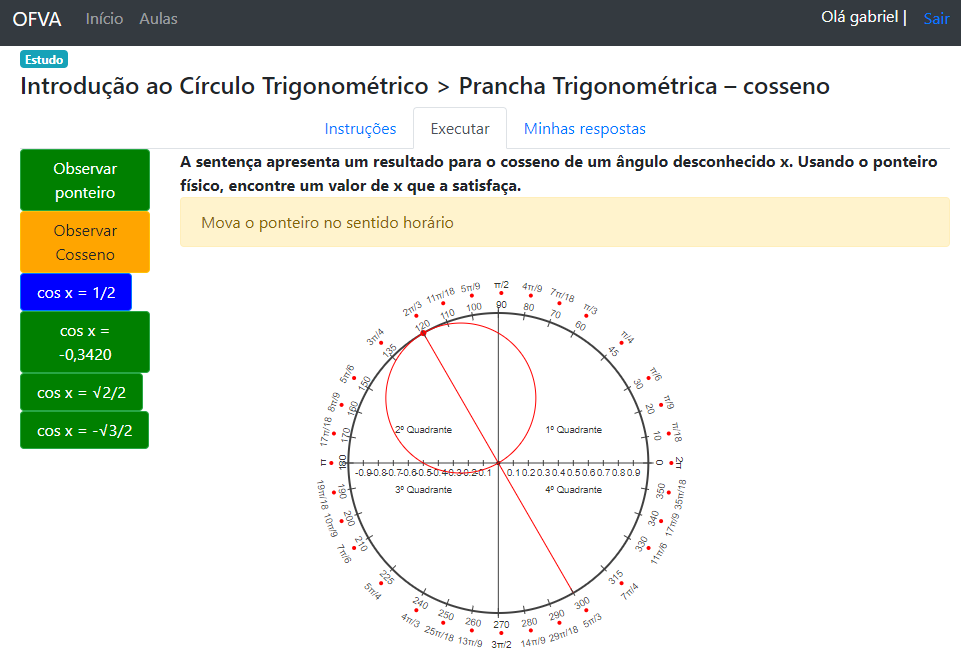
\includegraphics[width=0.9\linewidth]{chapters/results/Fase 3/E4_Virtual.png}
	\caption{Exercício 4 - Cosseno}
	\label{fig:E4}
\end{figure}

O formulário que descreve os elementos (aspectos educacionais, dispositivos, recursos, serviços, entradas/saídas e casos de teste) desta implementação do objeto tangível estão no Apêndice~\ref{Chap:AppendixCosseno} e a descrição dos elementos para os analíticos de aprendizagem para cada caso de teste estão no Apêndice~\ref{Chap:AppendixAnaliticosA04}.

\textbf{Nota Tradicional - $NT$}

A Tabela~\ref{tab:F3_A4_NT} apresenta as notas tradicionais relativas ao Exercício 4, onde é possível notar a ausência dos participantes $B02$, $B06$ e $B10$ que não iniciaram o exercício devido ao esgotamento do tempo de experimento.

\begin{table}[htbp]
	\centering
	\caption{$NT$ - Nota Tradicional}
	\begin{tabular}{|c|c|c|c|c|c|c|c|}
		\hline
		\rowcolor[HTML]{D9D9D9} 
		\textbf{Participante} & \textbf{C1} & \textbf{C2} & \textbf{C3} & \textbf{C4} & \textbf{C5} & \textbf{C6} & \textbf{NT} \\ \hline
		\rowcolor[HTML]{FFFFFF} 
		\textbf{B03} & 10.00 & 0.00 & 10.00 & 0.00 & 10.00 & 10.00 & 6.667 \\ \hline
		\rowcolor[HTML]{E7E6E6} 
		\textbf{B04} & 10.00 & 0.00 & 10.00 & 0.00 & 10.00 & 10.00 & 6.667 \\ \hline
		\rowcolor[HTML]{FFFFFF} 
		\textbf{B05} & 10.00 & 10.00 & 10.00 & 0.00 & 10.00 & 10.00 & 8.333 \\ \hline
		\rowcolor[HTML]{E7E6E6} 
		\textbf{B08} & 10.00 & 0.00 & 10.00 & 0.00 & 10.00 & 10.00 & 6.667 \\ \hline
		\rowcolor[HTML]{FFFFFF} 
		\textbf{B09} & 10.00 & 0.00 & 10.00 & 0.00 & 0.00 & 10.00 & 5.000 \\ \hline
		\rowcolor[HTML]{D9D9D9} 
		\textbf{NT Casos} & 10.00 & 2.00 & 10.00 & 0.00 & 8.00 & 10.00 & 6.667 \\ \hline
	\end{tabular}
	\label{tab:F3_A4_NT}
\end{table}

Com relação aos demais participantes, observou-se que a menor média de nota tradicional foi $5.00$ do participante $B09$, uma vez que tal indivíduo não finalizou os casos de teste $C2$, $C4$ e $C5$, enquanto o restante do grupo não finalizou os casos $C2$ e $C4$. Ainda neste sentido, sobressai-se o participante $B05$ que não finalizou somente o caso $C4$ e obteve maior média de $NT$, cujo valor foi de $8.333$.

O caso $C2$ é similar ao $C1$, onde ambos exigem que o participante manipule o ponteiro físico para inferir relações entre os valores de ângulo, quadrantes e cossenos, de modo que a explicação mais plausível sobre a dificuldade em responder $C2$ é que o índice de dificuldade deste caso (IDQ igual a 5) é superior ao de $C1$ (IDQ igual a 3). %não é possível afirmar uma dificuldade em específico com relação a isso, uma vez que todos finalizaram o caso $C1$.

O caso $C4$ corresponde a uma questão que aborda cosseno negativo, assim com o caso $C6$, de modo que não é possível inferir qualquer informação sobre isso, inclusive porque $C4$ aborda um valor de cosseno em número inteiro, enquanto $C6$ utiliza notação com radiciação, onde o IDQ de $C4$ é igual a 1 e o de $C6$ é igual a 3.

De todo modo, excluindo-se as semelhanças entre os conteúdos abordados nos casos e observando somente os valores de média de $NT$ para cada caso, nota-se que os casos $C2$ e $C4$ são os casos que os participantes tiveram maior dificuldade, embora, nesse momento, não seja possível encontrar as causas exatas para tal fato. Além disso, de acordo com a Tabela~\ref{tab:F3_A4_NT}, a média de $NT$ do grupo é $6.667$, de modo que somente $B09$ ficou abaixo desse valor.

\textbf{Nota Ponderada - $NP$}

Na Tabela~\ref{tab:F3_A4_NP} pode-se verificar que os participantes com menor média de nota ponderada são $B04$ e $B09$, cujas notas são $5.848$ e $5.253$ e, portanto, abaixo da média de $NP$ do grupo, cujo valor é $6.206$. Além disso, $B04$ teve desempenho abaixo da média do grupo nos casos $C1$ ($6.25$), $C3$ ($5.00$), $C4$ ($1.25$) e $C6$ ($6.67$), enquanto $B09$ obteve o mesmo desempenho nos casos $C2$ ($0.00$), $C3$ ($3.33$) e $C6$ ($5.68$). 

Por outro lado, o participante com melhor média de nota ponderada foi $B05$ com valor igual a $7.153$. Além disso, nota-se que este participante obteve pontuação igual a zero para o caso $C4$, sendo o único valor abaixo da média dos casos de teste obtido por este indivíduo.

\begin{table}[htbp]
	\centering
	\caption{$NP$ - Nota Ponderada - Modo Estudo}
	\begin{tabular}{|c|c|c|c|c|c|c|c|}
		\hline
		\rowcolor[HTML]{D9D9D9} 
		\textbf{Participante} & \textbf{C1} & \textbf{C2} & \textbf{C3} & \textbf{C4} & \textbf{C5} & \textbf{C6} & \textbf{NP} \\ \hline
		\rowcolor[HTML]{FFFFFF} 
		\textbf{B03} & 10.00 & 4.13 & 7.50 & 4.17 & 4.00 & 6.43 & 6.038 \\ \hline
		\rowcolor[HTML]{E7E6E6} 
		\textbf{B04} & 6.25 & 5.92 & 5.00 & 1.25 & 10.00 & 6.67 & 5.848 \\ \hline
		\rowcolor[HTML]{FFFFFF} 
		\textbf{B05} & 10.00 & 7.50 & 6.67 & 0.00 & 10.00 & 8.75 & 7.153 \\ \hline
		\rowcolor[HTML]{E7E6E6} 
		\textbf{B08} & 10.00 & 2.81 & 10.00 & 1.56 & 10.00 & 6.07 & 6.741 \\ \hline
		\rowcolor[HTML]{FFFFFF} 
		\textbf{B09} & 10.00 & 0.00 & 3.33 & 5.00 & 7.50 & 5.68 & 5.253 \\ \hline
		\rowcolor[HTML]{D9D9D9} 
		\textbf{NP Casos} & 9.25 & 4.07 & 6.50 & 2.40 & 8.30 & 6.72 & 6.206 \\ \hline
	\end{tabular}
	\label{tab:F3_A4_NP}
\end{table}

Com relação aos casos de teste, $C4$ foi o caso com menor média de $NP$ sendo igual a $2.40$, seguindo por $C2$ com $4.07$ e por $C3$ com $6.50$. %Vale ressaltar que assim como no Exercício 3, os casos de teste $C1$ e $C2$ abordaram manipulação e observação do ponteiro para inferência de conhecimentos sobre o relacionamento da posição do ângulo com o valor de cosseno, enquanto aos casos de $C3$ a $C6$ abordaram identificação de valores/posições de ângulo de acordo com valores de cosseno dados pela interface virtual.
Vale ressaltar que, tendo a nota tradicional apontado $C2$ e $C4$ como os mais problemáticos para os participantes, observar a nota ponderada no modo estudo permite posicionar $C4$ como o caso de teste que trouce mais dificuldade do que $C2$, ao comparar os valores de ambos os casos.

\begin{table}[htbp]
	\centering
	\caption{$NP$ - Modo Avaliação}
	\begin{tabular}{|c|c|c|c|c|c|c|c|}
		\hline
		\rowcolor[HTML]{D9D9D9} 
		\textbf{Participante} & \textbf{C1} & \textbf{C2} & \textbf{C3} & \textbf{C4} & \textbf{C5} & \textbf{C6} & \textbf{NP} \\ \hline
		\rowcolor[HTML]{FFFFFF} 
		\textbf{B03} & 10.00 & 5.00 & 10.00 & 0.00 & 10.00 & 10.00 & 7.500 \\ \hline
		\rowcolor[HTML]{E7E6E6} 
		\textbf{B04} & 10.00 & 7.50 & 10.00 & 0.00 & 10.00 & 10.00 & 7.917 \\ \hline
		\rowcolor[HTML]{FFFFFF} 
		\textbf{B05} & 10.00 & 10.00 & 10.00 & 0.00 & 10.00 & 10.00 & 8.333 \\ \hline
		\rowcolor[HTML]{E7E6E6} 
		\textbf{B08} & 10.00 & 2.50 & 10.00 & 0.00 & 10.00 & 10.00 & 7.083 \\ \hline
		\rowcolor[HTML]{FFFFFF} 
		\textbf{B09} & 10.00 & 0.00 & 10.00 & 0.00 & 5.00 & 10.00 & 5.833 \\ \hline
		\rowcolor[HTML]{D9D9D9} 
		\textbf{NP Casos} & 10.00 & 5.00 & 10.00 & 0.00 & 9.00 & 10.00 & 7.333 \\ \hline
	\end{tabular}
	\label{tab:F3_A4_NP_AVALIACAO}
\end{table}

A fim de complementar a exploração do desempenho dos participantes, a Tabela~\ref{tab:F3_A4_NP_AVALIACAO} exibe os dados relativos ao modo `avaliação' que, no contexto deste trabalho, é apresentado como uma alternativa a nota tradicional para avaliação da aprendizagem considerando um percurso sem \textit{feedback} automático com relação às respostas, isto é, sem levar em consideração o histórico de construção da aprendizagem (acertos e erros), mas, somente se o estudante concluiu ou não o exercício.

Desse modo, valores de $NP$ iguais a $10.00$ indicam que o participante concluiu o percurso com êxito (assim como na $NT$), enquanto valores menores do que $10.00$ indicam o quão perto da resposta correta o participante estava quando interrompeu o exercício. Além disso, é interessante notar que, no modo avaliação, todos os participantes obtiveram $NP$ igual a zero para $C4$.

\textbf{Prioridade - $P$}

A Tabela~\ref{tab:F3_A4_P} exibe os valores de Prioridade para os casos de teste e participantes do Exercício 4. Inicialmente, pode-se ressaltar que $P$ é igual a zero para os casos $C1$, $C3$, $C5$ (com exceção de $B09$) e $C6$ para todos os participantes se deve ao fato de que a $NT$ foi igual a $10$ em todas essas circunstâncias.

%no caso $C4$ os participantes não obtiveram nota tradicional igual a 10, a Tabela~\ref{tab:F3_A4_P} apresenta valores de prioridade somente para este caso. Embora o estudante $B09$ também não tenha obtido $10.00$ para o caso $C2$, a prioridade deste caso não pode ser calculada devido ao valor de nota proporcional ter sido igual a zero, indicando que o participante pode não ter respondido tal caso.

\begin{table}[htbp]
	\centering
	\caption{$P$ - Prioridade}
	\begin{tabular}{|c|c|c|c|c|c|c|c}
		\hline
		\rowcolor[HTML]{D9D9D9} 
		\textbf{Participante} & \textbf{C1} & \textbf{C2} & \textbf{C3} & \textbf{C4} & \textbf{C5} & \textbf{C6} & \multicolumn{1}{c|}{\cellcolor[HTML]{D9D9D9}\textbf{P}} \\ \hline
		\rowcolor[HTML]{FFFFFF} 
		\textbf{B03} & 0.00 & 4.13 & 0.00 & 4.17 & 0.00 & 0.00 & \multicolumn{1}{c|}{\cellcolor[HTML]{FFFFFF}2.01} \\ \hline
		\rowcolor[HTML]{E7E6E6} 
		\textbf{B04} & 0.00 & 5.92 & 0.00 & 1.25 & 0.00 & 0.00 & \multicolumn{1}{c|}{\cellcolor[HTML]{E7E6E6}1.95} \\ \hline
		\rowcolor[HTML]{FFFFFF} 
		\textbf{B05} & 0.00 & 0.00 & 0.00 & 0.00 & 0.00 & 0.00 & \multicolumn{1}{c|}{\cellcolor[HTML]{FFFFFF}1.19} \\ \hline
		\rowcolor[HTML]{E7E6E6} 
		\textbf{B08} & 0.00 & 2.81 & 0.00 & 1.56 & 0.00 & 0.00 & \multicolumn{1}{c|}{\cellcolor[HTML]{E7E6E6}2.25} \\ \hline
		\rowcolor[HTML]{FFFFFF} 
		\textbf{B09} & 0.00 & 0.00 & 0.00 & 5.00 & 7.50 & 0.00 & \multicolumn{1}{c|}{\cellcolor[HTML]{FFFFFF}2.63} \\ \hline
		\rowcolor[HTML]{D0CECE} 
		\textbf{P Casos} & 0.00 & 2.57 & 0.00 & 2.40 & 1.50 & 0.00 & \multicolumn{1}{c|}{\cellcolor[HTML]{D0CECE}2.005} \\ \hline
		\textbf{Desvio-Padrão} & 0.00 & 2.59 & 0.00 & 2.10 & 3.35 & 0.00 & \multicolumn{1}{l}{} \\ \cline{1-7}
	\end{tabular}
	\label{tab:F3_A4_P}
\end{table}

Assim, de acordo com a Tabela~\ref{tab:F3_A4_P}, considerando o todo do exercício, o participante com maior prioridade foi $B09$, seguido por $B08$ e, de modo contrário, $B05$ foi o participante com menor prioridade para o grupo estudado. Por fim, a prioridade média obtida pelo grupo foi de $2.005$.

Apesar de a média da prioridade de $C2$ ($2.57$) ser ligeiramente maior do que a de $C4$ ($2.40$), o desvio-padrão de $C4$ é menor do que de $C2$, o que indica que esta segunda amostra é mais homogênea, de modo que possível sugerir que $C4$ pode ser mais interessante de ser revisado pelo grupo do que $C2$, corroborando os achados de $NP$ nos modos estudo e avaliação. De fato, o único participante cuja prioridade é diferente de zero em $C4$ é $B5$, que também obteve o valor zero para $NP$, enquanto $C2$ contém dois participantes com $P$ igual a zero, onde $B05$ obteve $NT$ igual a dez e $B09$ obteve $NP$ igual a zero, impossibilitando o cálculo da prioridade.

\textbf{Dúvida - $D$}

A Tabela~\ref{tab:F3_A4_D} apresenta os dados relacionados à Dúvida dos casos de teste para os participantes $B03$, $B04$, $B05$, $B08$ e $B09$, onde o caso com maior média de dúvida foi $C2$ com valor igual a $12.60$. Apesar do desvio-padrão ter sido o mais elevado entre os casos, isso aconteceu devido ao participante $B09$ não ter respondido a questão ($-1$), enquanto o restante dos participantes obteve valores superiores à média do grupo com exceção de $B05$ cujo valor de Dúvida foi $9$.

\begin{table}[htbp]
	\centering
	\caption{$D$ - Dúvida}
	\begin{tabular}{|c|c|c|c|c|c|c|ccc}
		\hline
		\rowcolor[HTML]{D9D9D9} 
		\cellcolor[HTML]{D0CECE}\textbf{Participante} & \textbf{C1} & \textbf{C2} & \textbf{C3} & \textbf{C4} & \textbf{C5} & \textbf{C6} & \multicolumn{1}{c|}{\cellcolor[HTML]{D0CECE}\textbf{Total}} & \multicolumn{1}{c|}{\cellcolor[HTML]{D9D9D9}\textbf{Média}} & \multicolumn{1}{c|}{\cellcolor[HTML]{D9D9D9}\textbf{DP}} \\ \hline
		\cellcolor[HTML]{F2F2F2}\textbf{B03} & 0 & 22 & 1 & 11 & 4 & 6 & \multicolumn{1}{c|}{44} & \multicolumn{1}{c|}{7.33} & \multicolumn{1}{c|}{8.19} \\ \hline
		\rowcolor[HTML]{D9D9D9} 
		\textbf{B04} & 3 & 18 & 1 & 5 & 0 & 2 & \multicolumn{1}{c|}{\cellcolor[HTML]{D9D9D9}29} & \multicolumn{1}{c|}{\cellcolor[HTML]{D9D9D9}4.83} & \multicolumn{1}{c|}{\cellcolor[HTML]{D9D9D9}6.68} \\ \hline
		\cellcolor[HTML]{F2F2F2}\textbf{B05} & 0 & 9 & 2 & 1 & 0 & 1 & \multicolumn{1}{c|}{13} & \multicolumn{1}{c|}{2.17} & \multicolumn{1}{c|}{3.43} \\ \hline
		\rowcolor[HTML]{D9D9D9} 
		\textbf{B08} & 0 & 15 & 0 & 7 & 0 & 6 & \multicolumn{1}{c|}{\cellcolor[HTML]{D9D9D9}28} & \multicolumn{1}{c|}{\cellcolor[HTML]{D9D9D9}4.67} & \multicolumn{1}{c|}{\cellcolor[HTML]{D9D9D9}5.99} \\ \hline
		\cellcolor[HTML]{F2F2F2}\textbf{B09} & 1 & -1 & 2 & 2 & 1 & 10 & \multicolumn{1}{c|}{15} & \multicolumn{1}{c|}{2.50} & \multicolumn{1}{c|}{3.83} \\ \hline
		\cellcolor[HTML]{D9D9D9}\textbf{Dúvida Caso} & \cellcolor[HTML]{D9D9D9}0.80 & \cellcolor[HTML]{D9D9D9}12.60 & \cellcolor[HTML]{D9D9D9}1.20 & \cellcolor[HTML]{D9D9D9}5.20 & \cellcolor[HTML]{D9D9D9}1.00 & \cellcolor[HTML]{D9D9D9}5.00 & \multicolumn{1}{c|}{\cellcolor[HTML]{D9D9D9}25.80} & \multicolumn{1}{l}{} & \multicolumn{1}{l}{} \\ \cline{1-8}
		\textbf{Desvio-Padrão} & 1.30 & 8.96 & 0.84 & 4.02 & 1.73 & 3.61 & \multicolumn{1}{l}{} & \multicolumn{1}{l}{} & \multicolumn{1}{l}{} \\ \cline{1-7}
	\end{tabular}
	\label{tab:F3_A4_D}
\end{table}

É interessante notar que os casos de teste com menor valor médio são $C1$ e $C5$ cujos valores são $0.80$ e $1.00$, respectivamente. Além destes casos, pode-se citar também $C3$, cuja média é de $1.20$, como o caso com menor desvio-padrão ($0.84$). Estes três casos tem em comum os menores valores de média e desvio-padrão entre os casos analisados.

Com relação aos participantes, pode-se observar que o participante $B03$ obteve maior valor total de dúvida ($44$), seguido por $B04$ e $B05$ cujos valores obtidos são $29$ e $28$, respectivamente. Além disso, nota-se que o restante dos participantes do grupo obtiveram valores totais de dúvida abaixo da média do grupo ($25.80$).

Por fim, com relação a homogeneidade da distribuição dos valores de dúvida dos casos de teste, nota-se que os participantes com maior média de dúvida são também os com maior desvio-padrão, de modo que é possível observar que a média de $B03$ ($7.33$) foi influenciada pelos casos de teste $C2$ e $C4$, cujos valores de dúvida são iguais a $22$ e $11$, respectivamente.

\textbf{Nível de Assertividade - $A$}

Com relação à Assertividade, a Tabela~\ref{tab:F3_A4_A} apresenta os valores obtidos pelos participantes, de modo que todos obtiveram percentuais de $A$ abaixo de $50\%$, onde o menor valor foi do participante $B08$, correspondendo a $3\%$ de assertividade.

\begin{table}[htbp]
	\centering
	\caption{$A$ - Assertividade}
	\begin{tabular}{|c|c|c|c|c|c|c|c|}
		\hline
		\rowcolor[HTML]{D9D9D9} 
		\textbf{Participante} & \textbf{C1} & \textbf{C2} & \textbf{C3} & \textbf{C4} & \textbf{C5} & \textbf{C6} & \textbf{A} \\ \hline
		\rowcolor[HTML]{FFFFFF} 
		\textbf{B03} & 0.00 & 0.00 & 1.00 & 0.27 & 0.25 & 0.17 & 0.28 \\ \hline
		\rowcolor[HTML]{E7E6E6} 
		\textbf{B04} & 0.00 & 0.00 & 1.00 & 0.00 & 0.00 & 0.50 & 0.25 \\ \hline
		\rowcolor[HTML]{FFFFFF} 
		\textbf{B05} & 0.00 & 0.11 & 1.00 & 0.00 & 0.00 & 1.00 & 0.35 \\ \hline
		\rowcolor[HTML]{E7E6E6} 
		\textbf{B08} & 0.00 & 0.00 & 0.00 & 0.00 & 0.00 & 0.17 & 0.03 \\ \hline
		\rowcolor[HTML]{FFFFFF} 
		\textbf{B09} & 0.00 & 0.00 & 0.50 & 0.50 & 1.00 & 0.10 & 0.35 \\ \hline
		\rowcolor[HTML]{D0CECE} 
		\textbf{Média} & 0.00 & 0.02 & 0.70 & 0.15 & 0.25 & 0.39 & 0.25 \\ \hline
	\end{tabular}
	\label{tab:F3_A4_A}
\end{table}

O caso de teste com menor valor de $A$ foi $C1$, seguido por $C2$ e $C4$, onde de um modo geral, observa-se que os casos de teste relativos a manipulação do ponteiro físico para inferência de relações entre ângulos, quadrantes e cossenos obtiveram uma assertividade menor do que os casos de teste referentes a indicação dos ângulos relacionados a valores de cosseno. Por fim, a assertividade geral do grupo foi de aproximadamente $25\%$.

Por fim, o caso de teste com maior média de assertividade foi $C3$ cujo valor de $A$ foi de $70\%$, seguido por $C6$ com $39\%$.

\textbf{Níveis de Compreensão da Questão ($NCQ$) e do Questionário ($NC$)}

A Tabela~\ref{tab:F3_A4_NCQ} apresenta os valores de $NCQ$ e $NC$ para o grupo estudado neste exercício, de modo que o único participante a alcançar um nível de compreensão do questionário ($NC$) acima de $50\%$ e da média do grupo foi $B05$, que obteve $NC$ igual a $60.8\%$. Além disso, os participantes com $NC$ abaixo da média do grupo ($49.6\%$) foram $B09$, $B08$ e $B04$ com valores iguais a $42.6\%$, $47.5\%$ e $47.9\%$, respectivamente.

\begin{table}[htbp]
	\centering
	\caption{$NCQ$ e $NC$}
	\begin{tabular}{|c|cccccc|c|}
		\hline
		\rowcolor[HTML]{D0CECE} 
		\cellcolor[HTML]{D0CECE} & \multicolumn{6}{c|}{\cellcolor[HTML]{D0CECE}\textbf{NCQ}} & \cellcolor[HTML]{D0CECE} \\ \cline{2-7}
		\rowcolor[HTML]{D0CECE} 
		\multirow{-2}{*}{\cellcolor[HTML]{D0CECE}\textbf{Participante}} & \multicolumn{1}{c|}{\cellcolor[HTML]{D0CECE}\textbf{C1}} & \multicolumn{1}{c|}{\cellcolor[HTML]{D0CECE}\textbf{C2}} & \multicolumn{1}{c|}{\cellcolor[HTML]{D0CECE}\textbf{C3}} & \multicolumn{1}{c|}{\cellcolor[HTML]{D0CECE}\textbf{C4}} & \multicolumn{1}{c|}{\cellcolor[HTML]{D0CECE}\textbf{C5}} & \textbf{C6} & \multirow{-2}{*}{\cellcolor[HTML]{D0CECE}\textbf{NC}} \\ \hline
		\rowcolor[HTML]{FFFFFF} 
		\textbf{B03} & \multicolumn{1}{c|}{\cellcolor[HTML]{FFFFFF}1.000} & \multicolumn{1}{c|}{\cellcolor[HTML]{FFFFFF}0.393} & \multicolumn{1}{c|}{\cellcolor[HTML]{FFFFFF}0.644} & \multicolumn{1}{c|}{\cellcolor[HTML]{FFFFFF}0.263} & \multicolumn{1}{c|}{\cellcolor[HTML]{FFFFFF}0.367} & 0.621 & 0.489 \\ \hline
		\rowcolor[HTML]{E7E6E6} 
		\textbf{B04} & \multicolumn{1}{c|}{\cellcolor[HTML]{E7E6E6}0.625} & \multicolumn{1}{c|}{\cellcolor[HTML]{E7E6E6}0.559} & \multicolumn{1}{c|}{\cellcolor[HTML]{E7E6E6}0.339} & \multicolumn{1}{c|}{\cellcolor[HTML]{E7E6E6}0.074} & \multicolumn{1}{c|}{\cellcolor[HTML]{E7E6E6}0.970} & 0.665 & 0.479 \\ \hline
		\rowcolor[HTML]{FFFFFF} 
		\textbf{B05} & \multicolumn{1}{c|}{\cellcolor[HTML]{FFFFFF}0.999} & \multicolumn{1}{c|}{\cellcolor[HTML]{FFFFFF}0.736} & \multicolumn{1}{c|}{\cellcolor[HTML]{FFFFFF}0.524} & \multicolumn{1}{c|}{\cellcolor[HTML]{FFFFFF}0.000} & \multicolumn{1}{c|}{\cellcolor[HTML]{FFFFFF}0.969} & 0.813 & 0.608 \\ \hline
		\rowcolor[HTML]{E7E6E6} 
		\textbf{B08} & \multicolumn{1}{c|}{\cellcolor[HTML]{E7E6E6}0.992} & \multicolumn{1}{c|}{\cellcolor[HTML]{E7E6E6}0.271} & \multicolumn{1}{c|}{\cellcolor[HTML]{E7E6E6}0.882} & \multicolumn{1}{c|}{\cellcolor[HTML]{E7E6E6}0.059} & \multicolumn{1}{c|}{\cellcolor[HTML]{E7E6E6}0.630} & 0.480 & 0.475 \\ \hline
		\rowcolor[HTML]{FFFFFF} 
		\textbf{B09} & \multicolumn{1}{c|}{\cellcolor[HTML]{FFFFFF}1.000} & \multicolumn{1}{c|}{\cellcolor[HTML]{FFFFFF}0.000} & \multicolumn{1}{c|}{\cellcolor[HTML]{FFFFFF}0.299} & \multicolumn{1}{c|}{\cellcolor[HTML]{FFFFFF}0.375} & \multicolumn{1}{c|}{\cellcolor[HTML]{FFFFFF}0.733} & 0.428 & 0.426 \\ \hline
		\rowcolor[HTML]{D9D9D9} 
		\textbf{Média} & \multicolumn{1}{c|}{\cellcolor[HTML]{D9D9D9}0.923} & \multicolumn{1}{c|}{\cellcolor[HTML]{D9D9D9}0.392} & \multicolumn{1}{c|}{\cellcolor[HTML]{D9D9D9}0.538} & \multicolumn{1}{c|}{\cellcolor[HTML]{D9D9D9}0.154} & \multicolumn{1}{c|}{\cellcolor[HTML]{D9D9D9}0.734} & 0.601 & 0.496 \\ \hline
	\end{tabular}
	\label{tab:F3_A4_NCQ}
\end{table}

Por fim, o caso de teste $C4$ obteve uma média de $NCQ$ igual a $15.4\%$, sendo o menor valor dentre os casos de teste utilizados, seguido por $C2$ com $NCQ$ igual a $39.2\%$, de modo que este achado corrobora a interpretação de que os participantes tiveram mais dificuldades com $C4$ do que com $C2$, especialmente considerando que $C2$ possui naturalmente um índice de dificuldade mair do que $C4$.

\subsubsection{Exercício 5 - Tangente}\label{subsubsec:F3A5}

Assim como os exercícios 3 e 4, este exercício adapta uma questão relacionada a um aspecto do círculo trigonométrico, neste caso, a reta das tangentes. A interface física A05 está disponível na Seção~\ref{subsection:atividade3_A05} e os parâmetros da instância estão definidos no Apêndice~\ref{Chap:AppendixTangente}. Entretanto, diferentemente dos exercícios anteriores, este exercício não encontra um correspondente na atividade de fixação tradicional, de modo que seu conteúdo não foi abordado no pós-teste de ambos os grupos A e B.

\begin{figure}[htb]
	\centering
	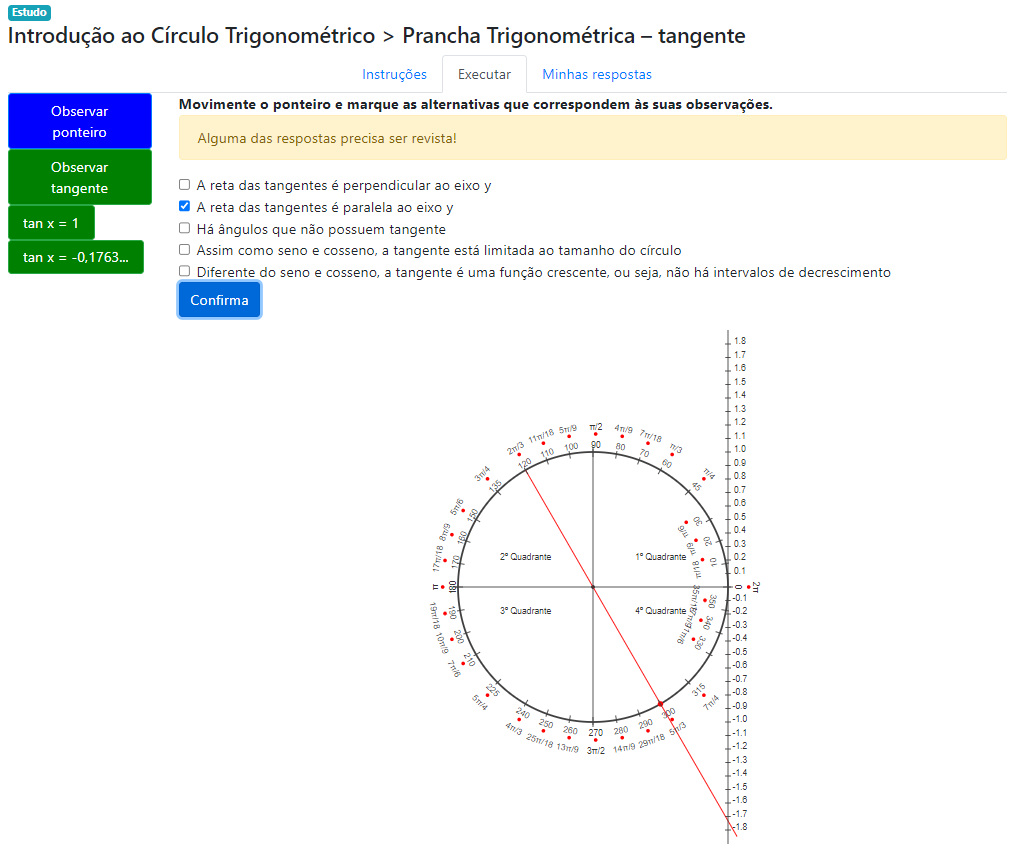
\includegraphics[width=0.9\linewidth]{chapters/results/Fase 3/E5_Virtual.png}
	\caption{Exercício 5 - Tangente}
	\label{fig:E5}
\end{figure}

\textbf{Nota Tradicional - $NT$}

A Tabela~\ref{tab:F3_A5_NT} apresenta as notas tradicionais relativas ao Exercício 5, onde é possível notar 

\begin{table}[htbp]
	\centering
	\caption{$NT$ - Nota Tradicional}
	\begin{tabular}{|c|c|c|c|c|c|}
		\hline
		\rowcolor[HTML]{D9D9D9} 
		\textbf{Participante} & \textbf{C1} & \textbf{C2} & \textbf{C3} & \textbf{C4} & \textbf{NT} \\ \hline
		\rowcolor[HTML]{FFFFFF} 
		\textbf{B03} & 10.00 & 10.00 & 10.00 & 10.00 & 10.00 \\ \hline
		\rowcolor[HTML]{E7E6E6} 
		\textbf{B04} & 0.00 & 10.00 & 10.00 & 10.00 & 7.50 \\ \hline
		\rowcolor[HTML]{FFFFFF} 
		\textbf{B05} & 10.00 & 10.00 & 0.00 & 10.00 & 7.50 \\ \hline
		\rowcolor[HTML]{E7E6E6} 
		\textbf{B08} & 0.00 & 10.00 & 10.00 & 10.00 & 7.50 \\ \hline
		\rowcolor[HTML]{FFFFFF} 
		\textbf{B09} & 0.00 & 0.00 & 10.00 & 10.00 & 5.00 \\ \hline
		\rowcolor[HTML]{D9D9D9} 
		\textbf{NT Casos} & 4.00 & 8.00 & 8.00 & 10.00 & 7.50 \\ \hline
	\end{tabular}
	\label{tab:F3_A5_NT}
\end{table}

\textbf{Nota Ponderada - $NP$}

Na Tabela~\ref{tab:F3_A5_NP_ESTUDO} pode-se verificar que 

\begin{table}[htbp]
	\centering
	\caption{$NP$ - Nota Ponderada - Modo Estudo}
	\begin{tabular}{|c|c|c|c|c|c|}
		\hline
		\rowcolor[HTML]{D9D9D9} 
		\textbf{Participante} & \textbf{C1} & \textbf{C2} & \textbf{C3} & \textbf{C4} & \textbf{NP} \\ \hline
		\rowcolor[HTML]{FFFFFF} 
		\textbf{B03} & 10.00 & 5.28 & 3.44 & 5.00 & 5.929 \\ \hline
		\rowcolor[HTML]{E7E6E6} 
		\textbf{B04} & 1.49 & 3.52 & 10.00 & 5.42 & 5.107 \\ \hline
		\rowcolor[HTML]{FFFFFF} 
		\textbf{B05} & 2.20 & 3.75 & 5.00 & 10.00 & 5.238 \\ \hline
		\rowcolor[HTML]{E7E6E6} 
		\textbf{B08} & 1.99 & 5.31 & 10.00 & 10.00 & 6.826 \\ \hline
		\rowcolor[HTML]{FFFFFF} 
		\textbf{B09} & 2.76 & 2.08 & 10.00 & 7.50 & 5.585 \\ \hline
		\rowcolor[HTML]{D9D9D9} 
		\textbf{NP Casos} & 3.69 & 3.99 & 7.69 & 7.58 & 5.737 \\ \hline
	\end{tabular}
	\label{tab:F3_A5_NP_ESTUDO}
\end{table}

\begin{table}[htbp]
	\centering
	\caption{$NP$ - Nota Ponderada - Modo Avaliação}
	\begin{tabular}{|c|c|c|c|c|c|}
		\hline
		\rowcolor[HTML]{D9D9D9} 
		\textbf{Participante} & \textbf{C1} & \textbf{C2} & \textbf{C3} & \textbf{C4} & \textbf{NP} \\ \hline
		\rowcolor[HTML]{FFFFFF} 
		\textbf{B03} & 10.00 & 10.00 & 10.00 & 10.00 & 10.000 \\ \hline
		\rowcolor[HTML]{E7E6E6} 
		\textbf{B04} & 0.00 & 10.00 & 10.00 & 10.00 & 7.500 \\ \hline
		\rowcolor[HTML]{FFFFFF} 
		\textbf{B05} & 10.00 & 10.00 & 0.00 & 10.00 & 7.500 \\ \hline
		\rowcolor[HTML]{E7E6E6} 
		\textbf{B08} & 2.50 & 10.00 & 10.00 & 10.00 & 8.125 \\ \hline
		\rowcolor[HTML]{FFFFFF} 
		\textbf{B09} & 7.50 & 2.50 & 10.00 & 10.00 & 7.500 \\ \hline
		\rowcolor[HTML]{D9D9D9} 
		\textbf{NP Casos} & 6.00 & 8.50 & 8.00 & 10.00 & 8.125 \\ \hline
	\end{tabular}
	\label{tab:F3_A5_NP_AVALIACAO}
\end{table}

\textbf{Prioridade - $P$}

A Tabela~\ref{tab:F3_A5_P} exibe os valores de Prioridade para os casos de teste e participantes do Exercício 4. Inicialmente, pode-se ressaltar que 

\begin{table}[htbp]
	\centering
	\caption{$P$ - Prioridade}
	\begin{tabular}{|c|c|c|c|c|c}
		\hline
		\rowcolor[HTML]{D9D9D9} 
		\textbf{Participante} & \textbf{C1} & \textbf{C2} & \textbf{C3} & \textbf{C4} & \multicolumn{1}{c|}{\cellcolor[HTML]{D9D9D9}\textbf{P}} \\ \hline
		\rowcolor[HTML]{FFFFFF} 
		\textbf{B03} & 0.00 & 0.00 & 0.00 & 0.00 & \multicolumn{1}{c|}{\cellcolor[HTML]{FFFFFF}0.00} \\ \hline
		\rowcolor[HTML]{E7E6E6} 
		\textbf{B04} & 1.49 & 0.00 & 0.00 & 0.00 & \multicolumn{1}{c|}{\cellcolor[HTML]{E7E6E6}1.28} \\ \hline
		\rowcolor[HTML]{FFFFFF} 
		\textbf{B05} & 0.00 & 0.00 & 5.00 & 0.00 & \multicolumn{1}{c|}{\cellcolor[HTML]{FFFFFF}1.31} \\ \hline
		\rowcolor[HTML]{E7E6E6} 
		\textbf{B08} & 1.99 & 0.00 & 0.00 & 0.00 & \multicolumn{1}{c|}{\cellcolor[HTML]{E7E6E6}1.71} \\ \hline
		\rowcolor[HTML]{FFFFFF} 
		\textbf{B09} & 2.76 & 2.08 & 0.00 & 0.00 & \multicolumn{1}{c|}{\cellcolor[HTML]{FFFFFF}2.79} \\ \hline
		\rowcolor[HTML]{D0CECE} 
		\textbf{P Casos} & 1.25 & 0.42 & 1.00 & 0.00 & \multicolumn{1}{c|}{\cellcolor[HTML]{D0CECE}1.42} \\ \hline
		\cellcolor[HTML]{FFFFFF}\textbf{Desvio Padrão} & \cellcolor[HTML]{FFFFFF}1.23 & \cellcolor[HTML]{FFFFFF}0.93 & \cellcolor[HTML]{FFFFFF}2.24 & \cellcolor[HTML]{FFFFFF}0.00 & \multicolumn{1}{l}{} \\ \cline{1-5}
	\end{tabular}
	\label{tab:F3_A5_P}
\end{table}

\textbf{Dúvida ($D$)}

A Tabela~\ref{tab:F3_A5_D} apresenta os valores de dúvida para os casos de teste do Exercício 5, de modo que é possível reconhecer os mesmos participantes que fizeram o Exercício 4. Além disso, nota-se que o grupo obteve um valor médio de dúvida de $75.20$.

\begin{table}[htbp]
	\centering
	\caption{$D$ - Dúvida}
	\begin{tabular}{|c|c|c|c|c|ccc}
		\hline
		\rowcolor[HTML]{D0CECE} 
		\textbf{Participante} & \textbf{C1} & \textbf{C2} & \textbf{C3} & \textbf{C4} & \multicolumn{1}{c|}{\cellcolor[HTML]{D0CECE}\textbf{Total}} & \multicolumn{1}{c|}{\cellcolor[HTML]{D0CECE}\textbf{Média}} & \multicolumn{1}{c|}{\cellcolor[HTML]{D0CECE}\textbf{DP}} \\ \hline
		\textbf{B03} & 0 & 8 & 7 & 2 & \multicolumn{1}{c|}{17} & \multicolumn{1}{c|}{4.25} & \multicolumn{1}{c|}{3.86} \\ \hline
		\rowcolor[HTML]{D0CECE} 
		\textbf{B04} & 103 & 21 & 0 & 5 & \multicolumn{1}{c|}{\cellcolor[HTML]{D0CECE}129} & \multicolumn{1}{c|}{\cellcolor[HTML]{D0CECE}32.25} & \multicolumn{1}{c|}{\cellcolor[HTML]{D0CECE}48.01} \\ \hline
		\textbf{B05} & 91 & 23 & 1 & 0 & \multicolumn{1}{c|}{115} & \multicolumn{1}{c|}{28.75} & \multicolumn{1}{c|}{42.84} \\ \hline
		\rowcolor[HTML]{D0CECE} 
		\textbf{B08} & 68 & 7 & 0 & 0 & \multicolumn{1}{c|}{\cellcolor[HTML]{D0CECE}75} & \multicolumn{1}{c|}{\cellcolor[HTML]{D0CECE}18.75} & \multicolumn{1}{c|}{\cellcolor[HTML]{D0CECE}33.00} \\ \hline
		\textbf{B09} & 28 & 11 & 0 & 1 & \multicolumn{1}{c|}{40} & \multicolumn{1}{c|}{10.00} & \multicolumn{1}{c|}{12.99} \\ \hline
		\cellcolor[HTML]{D0CECE}\textbf{Dúvida Caso} & \cellcolor[HTML]{D0CECE}58.00 & \cellcolor[HTML]{D0CECE}14.00 & \cellcolor[HTML]{D0CECE}1.60 & \cellcolor[HTML]{D0CECE}1.60 & \multicolumn{1}{c|}{\cellcolor[HTML]{D0CECE}75.20} & \multicolumn{1}{l}{} & \multicolumn{1}{l}{} \\ \cline{1-6}
		\textbf{Desvio-Padrão} & 43.24 & 7.48 & 3.05 & 2.07 & \multicolumn{1}{l}{} & \multicolumn{1}{l}{} & \multicolumn{1}{l}{} \\ \cline{1-5}
	\end{tabular}
	\label{tab:F3_A5_D}
\end{table}

O caso de teste $C1$ foi o caso com maior valor de dúvida, sendo igual a $58.00$ com desvio-padrão de $43.24$, de modo que é possível notar que enquanto os dois participantes com maior valor de dúvida obtiveram valores próximos a $100$, os dois com menor valor receberam $0$ e $28$. Essa disparidade de valores pode indicar que os participantes $B04$ e $B05$ tiveram mais dificuldade para chegar às respostas corretas sobre a tangente do que os outros indivíduos do grupo. 

Além disso, embora $C3$ e $C4$ tenham o mesmo valor médio de dúvida, nota-se que o desvio-padrão de ambos é diferente, de modo que é possível inferir que no caso $C4$, cujo desvio é menor, há uma maior distribuição dos valores de dúvida entre os indivíduos. Isso é confirmado ao observar a dúvida do participante $B03$ no caso $C3$ que é igual a $7$, enquanto para todos os outros indivíduos (com exceção de $B05$ com dúvida igual a 1), a dúvida do caso de teste é igual a zero. De modo que é possível, intuir que este participante foi quem obteve mais dificuldade para chegar a resposta correta durante o processo de construção do conhecimento acerca da relação entre a tangente e a posição de um ângulo no círculo trigonométrico.

Embora $B03$ tenha tido mais dificuldade no caso $C3$ do que o restante do grupo, este participante foi o que obteve menor valor médio de dúvida para a atividade, sendo um valor total de $17$, com média igual a $4.25$ e um desvio-padrão de $3.86$. 

Por outro lado, os participantes com maior valor médio de dúvida foram $B04$ e $B05$, com valores totais iguais a $129$ e $115$, além de média igual a $32.25$ e $28.75$, respectivamente. Ademais, é importante notar que ambos possuem também os maiores valores de desvio-padrão, indicando que a dúvida prevaleceu em menos questões e não na atividade como um todo, o que se pode confirmar observando seus valores de dúvida para os casos $C1$ e $C2$.

\textbf{Nível de Assertividade - $A$}

Com relação à Assertividade, a Tabela~\ref{tab:F3_A5_A} apresenta os valores obtidos pelos participantes, de modo que

\begin{table}[htbp]
	\centering
	\caption{$A$ - Assertividade}
	\begin{tabular}{|c|c|c|c|c|c|}
		\hline
		\rowcolor[HTML]{D9D9D9} 
		\textbf{Participante} & \textbf{C1} & \textbf{C2} & \textbf{C3} & \textbf{C4} & \textbf{A} \\ \hline
		\rowcolor[HTML]{FFFFFF} 
		\textbf{B03} & 0.00 & 0.00 & 0.14 & 0.50 & 0.16 \\ \hline
		\rowcolor[HTML]{E7E6E6} 
		\textbf{B04} & 0.00 & 0.00 & 0.00 & 0.40 & 0.10 \\ \hline
		\rowcolor[HTML]{FFFFFF} 
		\textbf{B05} & 0.00 & 0.00 & 1.00 & 0.00 & 0.25 \\ \hline
		\rowcolor[HTML]{E7E6E6} 
		\textbf{B08} & 0.00 & 0.00 & 0.00 & 0.00 & 0.00 \\ \hline
		\rowcolor[HTML]{FFFFFF} 
		\textbf{B09} & 0.00 & 0.00 & 0.00 & 1.00 & 0.25 \\ \hline
		\rowcolor[HTML]{D0CECE} 
		\textbf{Média} & 0.00 & 0.00 & 0.23 & 0.38 & 0.15 \\ \hline
	\end{tabular}
	\label{tab:F3_A5_A}
\end{table}

\textbf{Níveis de Compreensão da Questão ($NCQ$) e do Questionário ($NC$)}

A Tabela~\ref{tab:F3_A5_NCQ} apresenta os valores de $NCQ$ e $NC$ para o grupo estudado neste exercício, de modo que


\begin{table}[htbp]
	\centering
	\caption{$NCQ$ e $NC$}
	\begin{tabular}{|c|cccc|c|}
		\hline
		\rowcolor[HTML]{D9D9D9} 
		\cellcolor[HTML]{D9D9D9} & \multicolumn{4}{c|}{\cellcolor[HTML]{D9D9D9}\textbf{NCQ}} & \cellcolor[HTML]{D9D9D9} \\ \cline{2-5}
		\rowcolor[HTML]{D9D9D9} 
		\multirow{-2}{*}{\cellcolor[HTML]{D9D9D9}\textbf{Participante}} & \multicolumn{1}{c|}{\cellcolor[HTML]{D9D9D9}\textbf{C1}} & \multicolumn{1}{c|}{\cellcolor[HTML]{D9D9D9}\textbf{C2}} & \multicolumn{1}{c|}{\cellcolor[HTML]{D9D9D9}\textbf{C3}} & \textbf{C4} & \multirow{-2}{*}{\cellcolor[HTML]{D9D9D9}\textbf{NC}} \\ \hline
		\rowcolor[HTML]{FFFFFF} 
		\textbf{B03} & \multicolumn{1}{c|}{\cellcolor[HTML]{FFFFFF}1.000} & \multicolumn{1}{c|}{\cellcolor[HTML]{FFFFFF}0.474} & \multicolumn{1}{c|}{\cellcolor[HTML]{FFFFFF}0.208} & 0.477 & 0.446 \\ \hline
		\rowcolor[HTML]{E7E6E6} 
		\textbf{B04} & \multicolumn{1}{c|}{\cellcolor[HTML]{E7E6E6}0.076} & \multicolumn{1}{c|}{\cellcolor[HTML]{E7E6E6}0.292} & \multicolumn{1}{c|}{\cellcolor[HTML]{E7E6E6}0.570} & 0.372 & 0.267 \\ \hline
		\rowcolor[HTML]{FFFFFF} 
		\textbf{B05} & \multicolumn{1}{c|}{\cellcolor[HTML]{FFFFFF}0.128} & \multicolumn{1}{c|}{\cellcolor[HTML]{FFFFFF}0.253} & \multicolumn{1}{c|}{\cellcolor[HTML]{FFFFFF}0.439} & 0.956 & 0.374 \\ \hline
		\rowcolor[HTML]{E7E6E6} 
		\textbf{B08} & \multicolumn{1}{c|}{\cellcolor[HTML]{E7E6E6}0.158} & \multicolumn{1}{c|}{\cellcolor[HTML]{E7E6E6}0.491} & \multicolumn{1}{c|}{\cellcolor[HTML]{E7E6E6}0.909} & 0.910 & 0.494 \\ \hline
		\rowcolor[HTML]{FFFFFF} 
		\textbf{B09} & \multicolumn{1}{c|}{\cellcolor[HTML]{FFFFFF}0.203} & \multicolumn{1}{c|}{\cellcolor[HTML]{FFFFFF}0.169} & \multicolumn{1}{c|}{\cellcolor[HTML]{FFFFFF}0.933} & 0.724 & 0.427 \\ \hline
		\rowcolor[HTML]{D9D9D9} 
		\textbf{Média} & \multicolumn{1}{c|}{\cellcolor[HTML]{D9D9D9}0.313} & \multicolumn{1}{c|}{\cellcolor[HTML]{D9D9D9}0.336} & \multicolumn{1}{c|}{\cellcolor[HTML]{D9D9D9}0.612} & 0.688 & 0.402 \\ \hline
	\end{tabular}
	\label{tab:F3_A5_NCQ}
\end{table}


%\section{Mapeamentos Sistemáticos}\label{sec:resultados:mapeamentos}
%
%Conforme apresentado na Seção~\ref{sec:metodologia} (Método da Pesquisa), para este projeto estão previstos dois Mapeamentos Sistemáticos da Literatura (MSL). O primeiro mapeamento foi sobre recomendação de recursos pedagógicos e computação cognitiva e o segundo sobre sistemas ciber-físicos no contexto educacional. Nas próximas seções abordaremos cada um deles.
%
%\subsection{Computação Cognitiva e Recomendação de recursos educacionais}\label{sec:msl1}
%
%O primeiro mapeamento da literatura abordou a recomendação de atividades no contexto de sistemas cognitivos e gerou uma publicação na conferência de Qualis B1 \textit{Frontiers in Education}~\citep{leitao:2018}, 
%% intitulada ``\textit{Survey on Pedagogical Resources Recommendation using Cognitive Computing Systems}''
%tendo recentemente recebido uma citação em publicação de terceiros~\citep{coccoli:2019}.
%
%A Tabela~\ref{tab:compcog} apresenta resumidamente os objetivos do MSL executado. Além disso, a questão principal de pesquisa foi: ``Como recomendar atividades pedagógicas usando sistemas cognitivos durante o processo de ensino-aprendizagem?''.
%
%\begin{table}[htbp]
%\centering
%\caption{Objetivos do MSL - Computação Cognitiva}
%\begin{tabular}{|l|l|}
%\hline
%\textbf{Analisar} & Trabalhos que mostram sistemas cognitivos \\ \hline
%\textbf{Com o objetivo de} & \begin{tabular}[c]{@{}l@{}}Identificar paradigmas e abordagens pedagógicas, técnicas, \\ferramentas e objetos de aprendizagem\end{tabular} \\ \hline
%\textbf{No que diz respeito à} & \begin{tabular}[c]{@{}l@{}}Recomendação de atividades pedagógicas utilizando computação \\ cognitiva\end{tabular} \\ \hline
%\end{tabular}
%\label{tab:compcog}
%\end{table}
%
%Em vistas de resolver o problema tratado, foram definidas outras quatro questões secundárias, conforme a Tabela~\ref{tab:compcog_RQ}. Além disso, a Figura~\ref{fig:stringMSL} apresenta a \textit{string} de busca dentro do formato PICO (População, Intervenção, Comparação e Resultados).
%
%\begin{table}[htbp]
%\caption{Questões de Pesquisa - Computação Cognitiva}
%\begin{tabular}{|l|l|}
%\hline
%\multicolumn{1}{|c|}{\textbf{Questão}} & \multicolumn{1}{c|}{\textbf{Descrição}} \\ \hline
%\textbf{RQ1} & \begin{tabular}[c]{@{}l@{}}Que abordagens pedagógicas foram usadas na implementação de sistemas de \\ recomendação no contexto educacional?\end{tabular} \\ \hline
%\textbf{RQ2} & \begin{tabular}[c]{@{}l@{}}Que técnicas e ferramentas foram usadas na recomendação de objetos de \\ aprendizagem ou atividades pedagógicas?\end{tabular} \\ \hline
%\textbf{RQ3} & Que atividades pedagógicas ou objetos de aprendizagem foram recomendados? \\ \hline
%\textbf{RQ4} & \begin{tabular}[c]{@{}l@{}}Quais trabalhos fazem recomendações a partir do contexto da educação presencial e\\  a distância?\end{tabular} \\ \hline
%\end{tabular}
%\label{tab:compcog_RQ}
%\end{table}
%
%As publicações foram recuperadas a partir das bibliotecas digitais \textit{Scopus} e \textit{Engineering Village}. Sendo que no primeiro filtro, foram retornados 348 publicações, sendo 153 da Scopus e 195 da Engineering Village. Além disso, foram excluídos 47 arquivos duplicados, resultando um total de 301 artigos para o segundo filtro. Destes, apenas 19 publicações foram aceitas para extração. Como informação adicional foi calculado o Kappa de Cohen que apresentou cerca de 79.47\%, o que significa uma concordância substancial.
%
%\begin{figure}[ht]
%	\centering
%	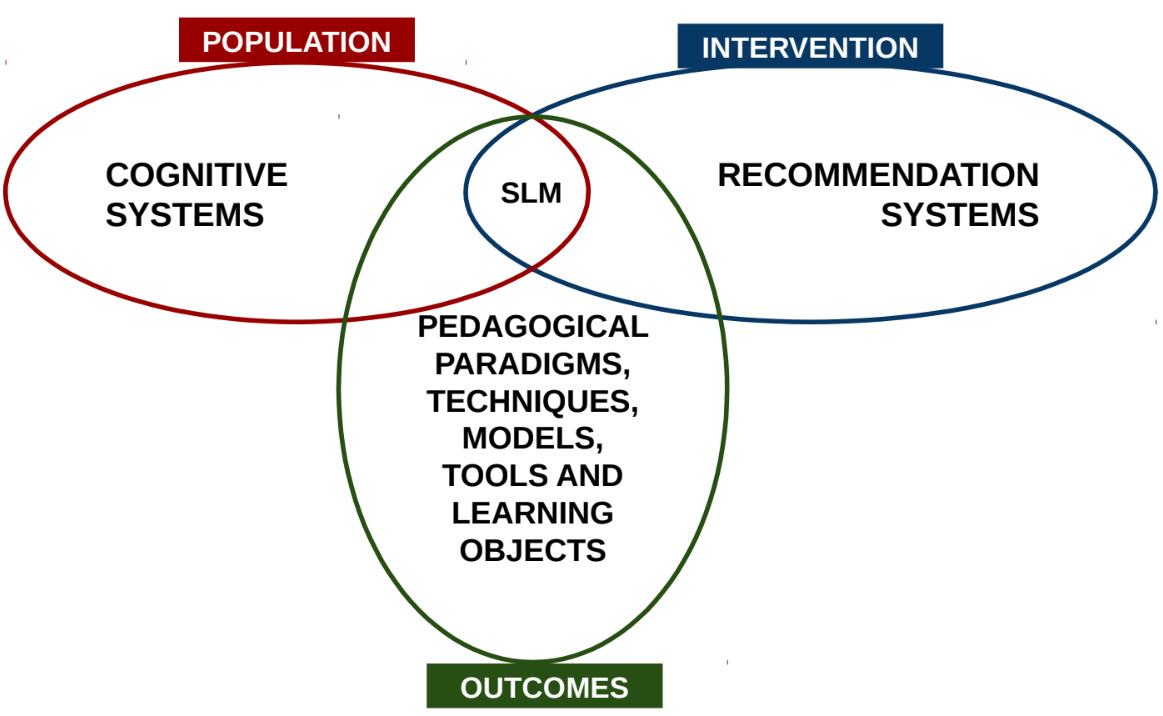
\includegraphics[width=0.9\linewidth]{imgs/MSL_string.png}
%	\caption{String de Busca - MSL}
%	\label{fig:stringMSL}
%\end{figure}
%
%A Figura~\ref{fig:MSL_publicacoes} o histórico de publicações envolvendo o uso de computação cognitiva na educação para recomendação ao longo dos últimos anos. Além disso, desse total, foi identificado que três autores publicaram 6 trabalhos nessa área nesse intervalo de tempo.
%
%\begin{figure}[ht]
%	\centering
%	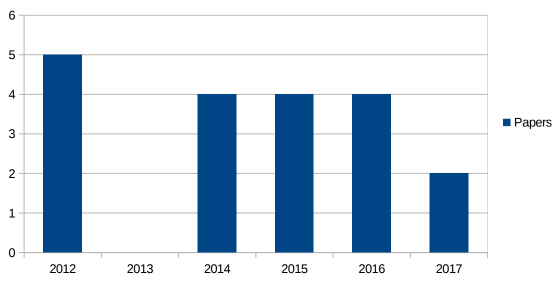
\includegraphics[width=0.9\linewidth]{imgs/MSL1_paperpeyear.png}
%	\caption{MSL - Publicações por ano}
%	\label{fig:MSL_publicacoes}
%\end{figure}
%
%Com relação a primeira questão de pesquisa (RQ1): \textbf{``Que abordagens pedagógicas foram usadas na implementação de sistemas de recomendação no contexto educacional?''}. Foi identificado que 9 publicações (47,37\%) tem relação com a abordagem humanista, 5 artigos (26,32\%) com abordagem cognitivista, 3 artigos (15,79\%) eram relativos a abordagem tradicional, 2 artigos (10,53\%) tinham uma abordagem comportamentalista e nenhum artigo trabalhava a abordagem sociocultural.
%
%Além disso, a maioria os artigos usava uma abordagem baseada em reconhecimento de emoções para tomada de decisão e não foram identificados estudos que ajudassem a entender como os alunos organizam o conhecimento, processam informações ou como o comportamento influencia sua tomada de decisão.
%
%A segunda questão de pesquisa (RQ2): \textbf{``Que técnicas e ferramentas foram usadas na recomendação de objetos de aprendizagem ou atividades pedagógicas?''} ajudou a identificar que alguns trabalhos não usaram apenas uma técnica, mas, uma combinação delas e que a maior parte das abordagens de detecção de emoção tem usado processamento de linguagem natural para isso. Além disso, a maioria dos trabalhos (12 artigos) utiliza técnicas de similaridades/correlação para fazer a recomendação, enquanto alguns artigos utilizaram técnicas de aprendizagem de máquina para isso (8 trabalhos). Apenas 4 trabalhos não informaram técnicas que usaram.
%
%Com relação às ferramentas, foi identificado que as ferramentas mais usadas são: IBM Watson, Facebook API, Apache Hadoop, Apache Mahout and Kinect Sensor/Framework, Repositórios de Objetos de Aprendizagem (i.e. Merlot), diferentes linguagens de programação e ontologia.
%
%A terceira questão de pesquisa (RQ3), relativa a \textbf{quais atividades pedagógicas e objetos de aprendizagem tem sido recomendados}, evidenciou que a maioria dos trabalhos (5 artigos) fazem recomendação de jogos e atividades interativas, em seguida, um total de 4 publicações fazem recomendação de material textual (.doc, .txt, .PDF, páginas HTML, livros,...) e apenas um trabalho oferece ajuda personalizada em lições ou exercícios e um faz recomendação de vídeos. Além disso, é importante notar que 42,11\% das publicações não indicou claramente quais recursos pedagógicos são recomendados, reduzindo-se a apresentar apenas estratégias de recomendação.
%
%Por fim, a última questão de pesquisa, sobre se o contexto era educação presencial ou a distância, ajudou a identificar que a maioria dos trabalhos (10 publicações) tem se concentrado em recomendações para ambientes de educação a distância. Além disso, apenas uma publicação era claramente focada em ambientes de sala presenciais e 8 trabalhos não apresentaram elementos que permitisse identificar o seu contexto.
%
%Ao final da revisão, percebemos algumas lacunas que poderiam ser atacadas por trabalhos futuros nessa área, tais como: (i) ausência de trabalhos da abordagem sociocultural; (ii) há poucos trabalhos usando reconhecimento facial ou interação do usuário para detectar emoções; (iii) técnicas baseadas no desempenho do aluno ainda podem ser exploradas (apenas cerca de 9\% recomendação de ajuda, lições e exercícios personalizados); (iv) oportunidades de trabalhar com a educação presencial; (v) recomendações baseadas em sensores físicos que permitam descobrir e analisar o comportamento dos estudantes.
%
%\subsection{Sistemas ciber-físicos no contexto educacional}
%
%O segundo mapeamento sistemático consiste em uma revisão da literatura com o objetivo de responder a questão: ``Como sistemas ciber-físicos tem sido utilizados nos processos de ensino-aprendizagem?'', tal como expresso nos objetivos condensados na Tabela~\ref{tab:MSL2_GQM}.
%
%\begin{table}[htbp]
%\centering
%\caption{Objetivos do MSL - Sistemas Físico-virtuais}
%\begin{tabular}{|l|l|}
%\hline
%\textbf{Analisar} & Sistemas físico-virtuais \\ \hline
%\textbf{Com o objetivo de} & \begin{tabular}[c]{@{}l@{}}Identificar paradigmas, teorias, objetos e atividades \\ pedagógicas, técnicas, ferramentas e disciplinas utilizadas\end{tabular} \\ \hline
%\textbf{No que diz respeito a} & Construção de ambientes de aprendizagem \\ \hline
%\textbf{Do ponto de vista do} & Pesquisador \\ \hline
%\textbf{No contexto} & Acadêmico \\ \hline
%\end{tabular}
%\label{tab:MSL2_GQM}
%\end{table}
%
%Assim, para esse mapeamento foram definidas quatro questões de pesquisa secundárias (Tabela~\ref{tab:MSL2_RQ}) no sentido de identificar as técnicas e ferramentas utilizadas na construção de sistemas físico-virtuais aplicados a educação.
%
%\begin{table}[htbp]
%\centering
%\caption{Questões de Pesquisa - Segundo MSL}
%\begin{tabular}{|l|l|}
%\hline
%\multicolumn{1}{|c|}{\textbf{Questão}} & \multicolumn{1}{c|}{\textbf{Descrição}} \\ \hline
%\textbf{RQ1} & \begin{tabular}[c]{@{}l@{}}Quais paradigmas ou teorias pedagógicas tem embasado o desenvolvimento de \\ sistemas físico-virtuais no contexto educacional?\end{tabular} \\ \hline
%\textbf{RQ2} & \begin{tabular}[c]{@{}l@{}}Quais técnicas e ferramentas tem sido utilizadas na construção de sistemas \\ físico-virtuais no contexto educacional?\end{tabular} \\ \hline
%\textbf{RQ3} & Quais atividades ou objetos de aprendizagem tem sido utilizados? \\ \hline
%\textbf{RQ4} & Quais disciplinas ou conteúdos tem sido abordados? \\ \hline
%\end{tabular}
%\label{tab:MSL2_RQ}
%\end{table}
%
%Devido ao ineditismo da proposta, a \textit{string} de busca foi adaptada para utilizar apenas dois conjuntos de modo a fazer uma prospecção mais profunda no universo de publicações relacionadas. Assim, foram utilizados somente os elementos população e intervenção do padrão PICO, que consistiram em ``sistemas ciber-físicos'' e ``ambientes de aprendizagem'', respectivamente, de modo que a \textit{string} de busca foi reduzida a: 
%
%$$(``cyber-physi*" \; OR\; (physic*\; AND\; (virtual\; OR\; cyber)))$$
%$$AND\; (teaching\; OR\; learning\; OR\; classroom))$$
%
%Esta \textit{string} retornou 4315 artigos, tendo sido 4000 provenientes da \textit{Scopus} e 315 da \textit{Science Direct}. Desse total, foram eliminados os artigos duplicados e sobraram 3467 publicações para o primeiro filtro, que consiste em ler `título', `resumo' e `palavras-chave'. Até o momento foram avaliadas 2268 publicações das quais 2055 foram rejeitadas e 213 passaram para o segundo filtro. Ainda falta avaliar um total de 1199 artigos.
%
%Vale ressaltar que dos 213 artigos que passaram para o segundo filtro já foram avaliadas 11 publicações, das quais 6 foram aceitas para a fase de extração e 5 foram rejeitadas.
%
%Por fim, os critérios de inclusão e exclusão que tem sido usados são apresentados na Tabela~\ref{tab:MSL2_CICE}.
%
%\begin{table}[htbp]
%\centering
%\caption{Critérios de Inclusão (CI) e Exclusão (CE)}
%\begin{tabular}{|l|l|}
%\hline
%\multicolumn{1}{|c|}{\textbf{Critérios}} & \multicolumn{1}{c|}{\textbf{Descrição}} \\ \hline
%\textbf{CI1} & Abordagens que utilizem sistemas físico-virtuais no contexto educacional \\ \hline
%\textbf{CE1} & Trabalho não é aplicável a nenhum critério de inclusão \\ \hline
%\textbf{CE2} & Publicação indisponível \\ \hline
%\textbf{CE3} & Coletânea de publicações \\ \hline
%\end{tabular}
%\label{tab:MSL2_CICE}
%\end{table}


%\section{Cronograma das atividades}\label{sec:cronograma}
%
%Esta proposta de Tese insere-se no contexto de um projeto de doutorado com duração prevista de quatro anos. Desse modo, a Tabela~\ref{Tabela:Objetos de Aprendizagem} apresenta as atividades do doutorado, onde as já concluídas estão marcadas com um `\textbf{X}', as atividades em andamento estão marcadas com um `\textbf{E}' e as futuras com `\textbf{P}'.
%
%A atividade 1 diz respeito às matérias obrigatórias do Programa de Pós-graduação em Informática da UFAM. A primeira parte da atividade 2 consistiu em levantar trabalhos que embasassem o primeiro mapeamento da literatura, enquanto a segunda parte levantou trabalhos para o segundo mapeamento. Além disso, a atividade 3 (primeiro mapeamento), como dito na Seção~\ref{sec:msl1}, teve como resultado a publicação de um artigo Qualis B1~\cite{leitao:2018}.
%
%Enquanto na atividade 5 foram revisadas e melhoradas as métricas de avaliação da aprendizagem herdadas do projeto anterior, além da definição de novas métricas, os trabalhos das atividades 4 e 6 consistiram em melhorias no protótipo anterior no que diz respeito a usabilidade do módulo Compositor, que permite geração de aulas com objetos de aprendizagem aceitos na versão atual da plataforma.
%
%A atividade 7 consiste em um novo mapeamento da literatura mais focado em buscar trabalhos relacionados a construção de ambientes de aprendizagem que utilizem objetos de aprendizagem físico-virtuais a fim de verificar o estado da arte e, assim, encontrar lacunas a serem trabalhadas, além de fundamentar o ineditismo deste projeto.
%
%A execução da atividade 8 deve resultar numa proposta de um sistema ciber-físico
%% multiagente 
%que esteja integrado a um ambiente de aprendizagem de modo que seja possível adicionar e utilizar objetos físico-virtuais de aprendizagem como parte processo de ensino-aprendizagem, incluindo a fase de avaliação de modo que seja possível realizar análise inteligente de aprendizagem e posterior recomendação de atividades pedagógicas. Tal proposta deve ser defendida na atividade 9 de Qualificação do Projeto. Após a defesa, o modelo poderá ser revisado e aprimorado, inclusive com a definição da linguagem de descrição a ser utilizada de maneira a facilitar a comunicação acerca dos estados dos componentes físicos.
%
%As atividades 11 e 12 serão executadas com vistas não apenas a testar as novas métricas, mas, a buscar maneiras de associá-las a objetos físico-virtuais de aprendizagem de modo que o uso de tais objetos sejam parte integrante do processo de ensino, inclusive fornecendo elementos para o acompanhamento automatizado e personalizado da aprendizagem dos estudantes. Tal integração é mais um passo em direção ao desenvolvimento da Educação 4.0.
%
%Enquanto as atividades 13 e 14 correspondem às implementações de componentes que provejam capacidade da plataforma de atuar com objetos físico-virtuais de aprendizagem nas fases de preparação e condução de uma aula, as atividades 15 e 16 dizem respeito às melhorias no módulo \textit{Analytics} relativas a tratar os dados de interação dos estudantes com os novos objetos físico-virtuais e a criação do módulo Inteligência que utilizará agentes inteligentes para notificar ou recomendar atividades pedagógicas.
%
%Vale ressaltar que um dos desafios no que concerne a recomendação envolvendo o uso de objetos de aprendizagem é a ausência de um repositório desses objetos e, igualmente, a ausência de uma base de dados de interação. Um ponto de partida para a resolução desse problema é a formalização e a implementação de mecanismos voltados a criação de objetos físico-virtuais. Além disso, este trabalho propôs um estudo de caso que permita validar a proposta de criação de objetos físico-virtuais de aprendizagem que esteja integrados a uma forma de verificação da aprendizagem através de métricas de avaliação.
%
%A atividade 17 consistirá em novos experimentos, com objetos de aprendizagem físico-virtuais incorporados ao sistema, enquanto a execução das atividades seguintes (18, 19 e 20) tem o objetivo de tratar os resultados dos experimentos e finalizar a tese de doutorado a ser defendida.
%
%
%% Please add the following required packages to your document preamble:
%% \usepackage{multirow}
%\begin{landscape}
%\begin{table}[ht]
%\centering
%\caption{Cronograma de Atividades do Doutorado}
%% \begin{adjustbox}{angle=90}
%\begin{tabular}{|c|l|c|c|c|c|c|c|c|c|c|c|c|c|c|c|c|c|c|c|}
%\hline
%\multirow{2}{*}{\textbf{Nº}} & \multicolumn{1}{c|}{\multirow{2}{*}{\textbf{Atividades}}} & \multicolumn{4}{c|}{\textbf{2017}} & \multicolumn{4}{c|}{\textbf{2018}} & \multicolumn{4}{c|}{\textbf{2019}} & \multicolumn{4}{c|}{\textbf{2020}} & \multicolumn{2}{c|}{\textbf{2021}} \\ \cline{3-20} 
% & \multicolumn{1}{c|}{} & \multicolumn{2}{c|}{\textbf{1/2017}} & \multicolumn{2}{c|}{\textbf{2/2017}} & \multicolumn{2}{c|}{\textbf{1/2018}} & \multicolumn{2}{c|}{\textbf{2/2018}} & \multicolumn{2}{c|}{\textbf{1/2019}} & \multicolumn{2}{c|}{\textbf{2/2019}} & \multicolumn{2}{c|}{\textbf{1/2020}} & \multicolumn{2}{c|}{\textbf{2/2020}} & \multicolumn{2}{c|}{\textbf{1/2021}} \\ \hline
%1 & Cumprimentos de Créditos & X & X & X & X & X & X &  &  &  &  &  &  &  &  &  &  &  &  \\ \hline
%2 & Pesquisa Bibliográfica Ad Hoc &  &  & X & X &  &  & X & X &  &  &  &  &  &  &  &  &  &  \\ \hline
%3 & Primeiro Mapeamento Sistemático &  &  &  &  &  &  & X & X & X & X &  &  &  &  &  &  &  &  \\ \hline
%4 & Modelagem dos Bancos de Dados &  &  &  & X & X & X & X & X & X &  &  &  &  &  &  &  &  &  \\ \hline
%5 & Analíticos e Métricas de Aprendizagem &  &  &  & X & X & X & X & X &  &  &  &  &  &  &  &  &  &  \\ \hline
%6 & Realização de Experimentos e Melhorias &  &  & X & X & X & X & X & X & E & E & P & P & P & P &  &  &  &  \\ \hline
%7 & Segundo Mapeamento Sistemático &  &  &  &  &  &  & X & X & E & E & P & P &  &  &  &  &  &  \\ \hline
%8 & Descrição Formal do Modelo Proposto &  &  &  &  &  &  &  &  &  & X & E & P &  &  &  &  &  &  \\ \hline
%9 & Qualificação do Projeto &  &  &  &  &  &  &  &  &  &  & E &  &  &  &  &  &  &  \\ \hline
%10 & Revisão e Melhorias no Modelo Proposto &  &  &  &  &  &  &  &  &  &  &  & P & P & P & P &  &  &  \\ \hline
%11 & Implementação - Analíticos e Métricas &  &  &  &  &  &  &  &  &  & E & P & P &  &  &  &  &  &  \\ \hline
%12 & Avaliação - Novos Analíticos e Métricas &  &  &  &  &  &  &  &  &  & P & P & P &  &  &  &  &  &  \\ \hline
%13 & Implementação Modelo Físico-virtual &  &  &  &  &  &  &  &  &  &  & P & P & P & P &  &  &  &  \\ \hline
%14 & Avaliação dos objetos físico-virtuais &  &  &  &  &  &  &  &  &  &  & P & P & P & P &  &  &  &  \\ \hline
%15 & Implementação Agentes e recomendações &  &  &  &  &  &  &  &  &  &  &  &  & P & P & P & P &  &  \\ \hline
%16 & Avaliação - Agentes e recomendações &  &  &  &  &  &  &  &  &  &  &  &  & P & P & P & P &  &  \\ \hline
%17 & Experimentos e Ajustes &  &  &  &  &  &  &  &  & P & P & P & P & P & P & P & P &  &  \\ \hline
%18 & Escrita de Artigos e Relatórios Técnicos &  &  & X & X & X & X & X & X & E & E & P & P & P & P & P & P & P &  \\ \hline
%19 & Redação do Documento da Tese &  &  &  &  &  &  &  &  &  &  &  &  &  &  & P & P & P &  \\ \hline
%20 & Defesa da Tese &  &  &  &  &  &  &  &  &  &  &  &  &  &  &  &  & P &  \\ \hline
%\end{tabular}
%% \end{adjustbox}
%\label{Tabela:Cronograma}
%\end{table}
%\end{landscape}


\newpage
% -----------------------------------------------------------------
% => Summary - PARTIAL RESULTS 
% -----------------------------------------------------------------
\section{Resumo}
\label{summary:PartialResults}

Este Capítulo apresentou alguns resultados experimentais de simulados do Exame Nacional do Ensino Médio contendo cerca de 40 questões e aplicados em turmas de um Instituto Federal, com o objetivo de coletar dados para validar as métricas propostas nesta tese, bem como apresentar algumas das possibilidades de análises e inferências acerca do desempenho escolar dos estudantes. Para essa discussão, foram utilizados somente os resultados de uma das turmas, contendo 33 estudantes.

Além disso, foi apresentado um método de agrupamento dos estudantes a partir da composição de das métricas `Grau de Assertividade' e `Nível de Compreensão'. Neste caso, considerando o valor comum utilizado para mensurar a aprovação dos estudantes no Brasil, em torno de 50\% da nota tradicional, nós classificamos os estudantes em 4 grupos considerando os quadrantes do Plano Cartesiano em função destas duas métricas. Assim, o primeiro quadrante contém os estudantes com ambas as métricas acima de 50\%, isto é, os estudante com bons níveis de compreensão e assertividade. Por outro lado, no terceiro quadrante, observamos os estudantes em situação oposta, ou seja, com compreensão e assertividade abaixo de 50\%. Sendo este último caso mais preocupante, os estudantes deste quadrante foram analisados com o objetivo de descobrir as razões de seu baixo desempenho. De um modo geral, esta análise nos permite concluir que os dados provenientes das novas métricas de aprendizagem podem ser úteis para gerar \textit{feedbacks} e recomendações.

Na Seção~\ref{sec:estudo_caso1}, foi apresentada uma proposta de Estudo de Caso cujo objetivo será validar e aprimorar a arquitetura proposta neste trabalho. Tal estudo consistirá na implementação de um objeto de aprendizagem físico-virtual seguida de coleta de dados. O objeto implementado será uma `máquina de somar', um brinquedo educacional que originalmente é um manipulativo físico voltado a ensinar noções de contagem e soma para crianças em idade escolar.

A Seção~\ref{sec:resultados:mapeamentos} apresentou detalhes dos dois mapeamentos sistemáticos previstos para esta pesquisa de doutorado. O primeiro mapeamento, relacionado ao uso de computação cognitiva para recomendação de recursos educacionais, já foi concluído e gerou uma publicação em conferência. O segundo mapeamento ainda está em fase de execução, mais precisamente no primeiro filtro.

%Por fim, a Seção~\ref{sec:cronograma} apresentou e detalhou o cronograma de atividades desta pesquisa.


% %Comentários relacionados com as respostas às questões de pesquisa
% Este capítulo apresentou resultados e discussões de experimentos feitos em sala de aula, com uma turma de estudantes de curso técnico em Informática. Tais experimentos tiveram o objetivo de ser um estudo de caso que validasse o método proposto por este trabalho, onde são introduzidos recursos computacionais que sirvam de suporte ao professor durante todo o processo de ensino-aprendizagem. Para isso, foram propostas questões de pesquisa que nortearam as análises feitas nas seções seguintes. Além disso, para melhor divisão e entendimento, o capítulo foi dividido em duas seções principais, seguindo o processo de construção de uma aula definido por~\cite{Zilse:2016} que distingue duas fases de Composição e Execução da Aula, onde a análises feitas sobre as aulas encontram-se na fase de Execução.

% A Seção~\ref{section:composicao_aula_experimental} detalhou o planejamento e a composição das aulas utilizadas no experimento. Nessa parte, o `Compositor' foi o meio através do qual a aula foi gerada utilizando diversos objetos de aprendizagem e definindo informações importantes para as métricas de análise da aprendizagem. Assim, foram inseridos os conteúdos da aula, as questões principais e secundárias e as sugestões utilizados nos questionários. Esta seção apresentou ainda estatísticas iniciais sobre as aulas, tais como os níveis de dificuldade e a distribuição proporcional dos conteúdos da aula.

% A Seção~\ref{section:aulaexperimental} apresentou resultados e discussões a partir das métricas propostas na Seção~\ref{section:analytics}. Tais discussões emergem como resultados diretos da inserção de recursos computacionais para coleta de dados e geração automática de gráficos. Esta seção contém duas subseções (\ref{section:analiseAula01} e~\ref{section:analiseAula02}) sobre as aulas experimento. Além disso, essas subseções contém análises sobre as métricas e sobre o uso de questões com ajuda sob demanda. 

% As Subseções~\ref{section:analise_pontuacao} e~\ref{section:analise_pontuacaoAula02} apresentaram a métrica tradicional de cálculo de pontos a partir do somatório dos valores das questões que cada aluno acertou. Ao longo das seções seguintes, ficou mais evidente a insuficiência dessa métrica como único ou principal mecanismo de avaliação do desempenho dos estudantes. O principal motivo é que a simples pontuação não fornece elementos suficientes para uma visão mais detalhada das dificuldades e características dos estudantes e da turma, diminuindo assim as possibilidades de o professor identificar e trabalhar melhor as demandas que surgem.

% As Subseções~\ref{section:analise_confusao} e~\ref{section:analise_confusaoAula02} apresentaram resultados e discussões relativos à métrica do Nível de Confusão que é baseada em quantas vezes uma questão teve a resposta marcada ou trocada pelo aluno. Esta métrica evidencia a incerteza da turma diante de uma questão e, ao ser associada à tabela do nível de dificuldade das questões, possibilita a rápida identificação de qual tópico precisa ser melhor trabalhado com a turma analisada. É importante recordar que a análise do Tempo de Resposta (tempo gasto na resolução de uma questão), cujos resultados foram discutidos nas Subseções~\ref{section:analise_temporesposta} e~\ref{section:analise_temporespostaAula02}, ajudou a confirmar a necessidade apontada anteriormente pelo Nível de Confusão.

% A métrica do nível de desordem evidencia a tendência da turma na resolução de um questionário avaliativo no que diz respeito à ordem em que as questões são consideradas resolvidas pelo estudante. Os resultados apresentados nas Subseções~\ref{section:analise_desordem} e~\ mostram evidências de que a ordem das questões, definida pelo professor na etapa de Composição da Aula, foi adequada para mais da metade da turma, quando esta recebeu ajuda sob demanda. De modo inverso, os alunos que não receberam ajuda sob demanda, tenderam a responder as questões que julgaram mais fáceis.

% Das métricas utilizadas neste trabalho, o nível de compreensão (Subseções~\ref{section:analise_compreensao} e~\ref{section:analise_compreensaoAula02}) contêm parâmetros que fornecem elementos sobre a aquisição de conhecimento a partir de um processo avaliativo, com mais detalhes do que a Pontuação tradicional. Levando em consideração os níveis de dificuldade do tópico, do conteúdo, da questão e o quão perto uma alternativa está da correta e em função do tempo de resposta, essa métrica possibilita ao professor verificar o nível de dificuldade dos estudantes, ou da turma, para resolver um conjunto de questões. O tempo é um fator muito importante dessa métrica, pois, caso o estudante ultrapasse um limiar pré-definido pelo professor, será penalizado no seu nível de compreensão. Assim, de acordo com essa métrica, para dois estudantes que escolheram a mesma alternativa de resposta, caso um responda dentro do tempo limite e outro ultrapasse, o segundo estudante será avaliado com menor nível de compreensão do que o primeiro.

% As Subseções~\ref{section:analise_uso_adaptacoes} e~\ref{section:analise_uso_adaptacoesAula02comajuda} discutem sobre a eficácia no desempenho dos estudantes do uso de ajuda sob demanda em questionários avaliativos, onde a partir dos resultados obtidos, foram encontrados indícios de que a abordagem proposta ajuda a melhorar os resultados obtidos pelos estudantes.